\documentclass[
    lang=cn,
    mode=simple,
    device=normal,
    chinesefont=founder,
    color=black,
    twoside,
    external=true
]{simplebook}

\linenumbers

\title{雷达信号处理中的矩阵方法}
\author{朱亮亮}
\includeonly{tex/signal.tex}
\begin{document}
\maketitle

\frontmatter
\pagenumbering{Roman}
\tableofcontents

\mainmatter
\pagenumbering{arabic}

\chapter{绪论}
\label{chp1}

\section{雷达的基本概念}
雷达是英文 Radio Detection and Ranging(Radar)的缩写的英译,即用无线电波的反射信号发现目标并测定其空间位置、移动方向、速度、相对距离以及大概形状的电子设备。作为一种重要的探测手段,雷达被广泛应用于航空与航海导航、军事侦察和预警、气象观测以及太空探索等领域。

严格来说,雷达的研发工作始于20世纪30年代,最初是为了探测敌方飞机和舰船而设计的,但雷达的基本概念却可以追溯到半个多世纪前。在1864年,麦克斯韦(James Clerk Maxwell)提出了电磁波的理论,给出了著名的麦克斯韦方程组,从理论上证明了光是一种特殊的电磁波。该理论的一个延伸是,电磁波也可以像电磁波一样被金属物体反射、被电介质折射。随后赫兹(Heinrich Hertz)在1887年使用波长为66厘米(对应于大约 455MHz)的无线电波成功地实验验证了这一结论,并于1888年发表了相关论文。

实验装置如\cref{fig_chp1_hertz}所示,主要由一个发射天线和一个接收天线组成。其中发射天线是由两个黄铜球连接的金属棒构成,中间留有一个小间隙。当接通电源时,电流在金属棒之间产生振荡,从而在空间中产生无线电波。这些无线电波会在空间中传播,并被金属板反射回来,形成驻波。接收天线则是一个有开口的金属环,它可以接收到反射回来的无线电波,并在开口处产生火花。通过移动接收天线的位置,可以观察到火花的强度变化,从而得到无线电波的波长,结合频率可以计算出电磁波的传播速度,进而验证麦克斯韦方程组的正确性。

\begin{figure}[htb!]
    \centering
    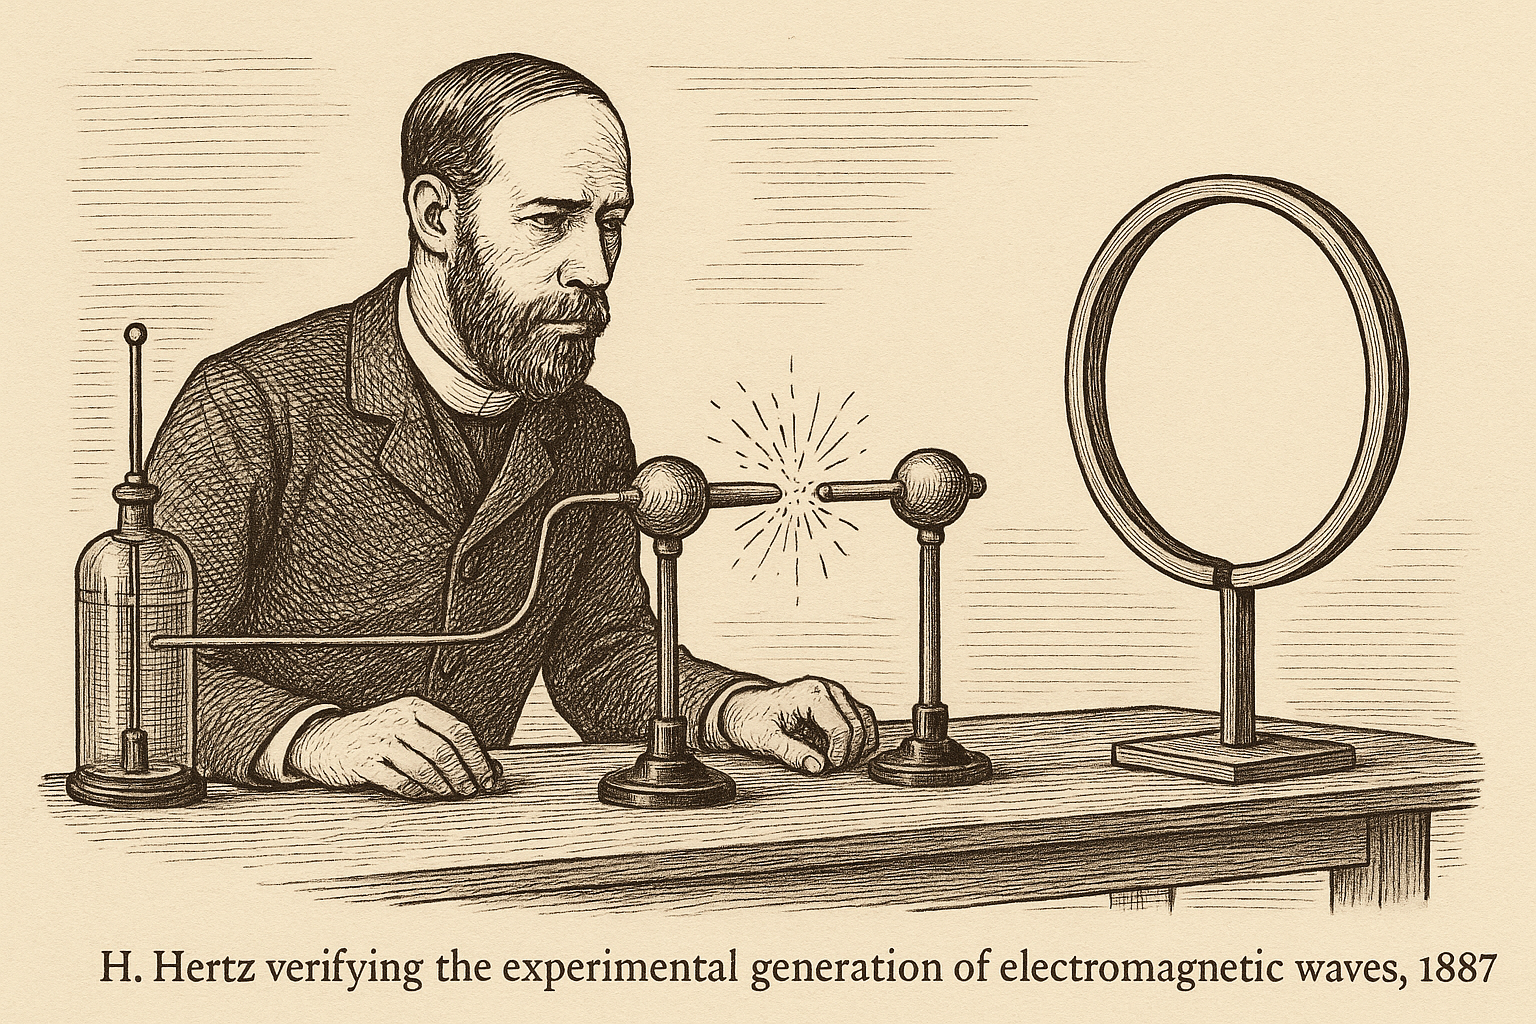
\includegraphics[width=.6\textwidth]{./img/intro/hertz_experiment.png}
    \caption{赫兹的实验装置示意图}
    \label{fig_chp1_hertz}
\end{figure}

雷达利用的便是电磁波的反射特性,通过发射电磁波并接收其反射信号来探测目标物体的位置、方位和速度等信息。雷达系统通常包括发射机、接收机、天线和信号处理单元等部分。发射机产生高频电磁波信号,通过天线向外发射。当电磁波遇到目标物体时,会发生反射,反射信号被天线接收并传输到接收机进行处理。通过分析反射信号的时间延迟和频率变化等特征,可以计算出目标物体的距离、速度和方向等信息。

\section{雷达工作原理}

\subsection{基本组成}
雷达系统的主要组成部分包括发射机、接收机、天线、波形产生器和信号处理单元等,如\cref{fig_chp1_radar_system}所示。

\begin{figure}[htb!]
    \centering
    % \includegraphics[width=.4\textwidth]{./img}
    \begin{tikzpicture}
        \tikzset{
            myblock/.style={
                rectangle, draw, minimum width=2cm, minimum height=1cm, rounded corners, thick
            }
        }

        \node (transmitter) [myblock, fill=c1!60] at (0, 0) {发射机};
        \node (receiver) [myblock, fill=c2!60] at (0, -3) {接收机};
        \node (antenna) [myblock, fill=c3!60] at (-3, -1.5) {天线};
        \node (waveform_generator) [myblock, fill=c4!60] at (3, 0) {波形产生器};
        \node (signal_processing) [myblock, fill=c5!60] at (3, -3) {信号处理单元};

        \draw[-latex, thick] (transmitter) -- (antenna);
        \draw[-latex, thick] (antenna) -- (receiver);
        \draw[-latex, thick] (receiver) -- (signal_processing);
        \draw[-latex, thick] (waveform_generator) -- (transmitter);
    \end{tikzpicture}
    \caption{雷达系统的基本组成}
    \label{fig_chp1_radar_system}
\end{figure}

整个雷达系统的工作流程如下:
\begin{enumerate}
    \item \textbf{波形产生}:波形产生器生成特定的电磁波信号,通常是脉冲信号或连续波信号。
    \item \textbf{发射}:发射机将生成的电磁波信号放大,并通过天线向外发射。
    \item \textbf{接收}:当电磁波遇到目标物体时,会发生反射,反射信号被天线接收并传输到接收机,接收机将接收到的信号进行放大和滤波,以提高信噪比。
    \item \textbf{信号处理}:信号处理单元对接收到的信号进行分析和处理,以提取目标信息,如距离、速度和方位等。
\end{enumerate}

最后,处理后的目标信息可以通过显示器或其他输出设备进行显示,同时可以根据需要进行控制和调整。

\subsection{工作频率}

雷达的工作频率范围非常广泛,从几千赫兹(kHz)到几百吉赫兹(GHz)不等。工程上将雷达的工作频率划分为多个频率,\cref{tab_chp1_radar_frequency}给出了常见的雷达工作频率范围、对应的波段名称以及主要应用场景和特点。

\begin{table}[htb!]
    \centering
    \caption{常见雷达工作频率范围及应用}
    \label{tab_chp1_radar_frequency}
    \small
    \begin{tabular}{c|c|p{7cm}}
        \hline
        波段名称 & 频率范围           & 主要应用场景和特点                                                                                                      \\
        \hline
        \hline
        HF   & 3 - 30 MHz     & 短波具有在地面与电离层之间多次反射的特性(天波),适用于超视距、超远程雷达工作;但电波传播稳定性差,电磁频谱拥挤,易受干扰,不易辨别真伪目标,一般雷达不采用
        \\
        \hline
        VHF  & 30 - 300 MHz   & 米波雷达具有大天线口径、高辐射功率、传播衰减小和不受气象条件影响和建造费用相对较低的优点。米波是监视卫星、洲际导弹的大型超远程雷达的重要波段。它也可用于一般简单的中、近程监视雷达。但频段频谱拥挤与通信频段猫短,一般较少用 \\ \hline
        UHF  & 300 - 1000 MHz & 适用于远程监视雷达,但因电视频段占用而很少采用                                                                                        \\
        \hline
        L    & 1 - 2 GHz      & 此频段的天线发射增益、天线口径、发射功率、接收机噪声性能、抗干扰性能等都较适中,是中、远程对空监视雷达常用的重要波段                                                     \\
        \hline
        S    & 2 - 4 GHz      & 为对空搜索监视雷达和导航雷达的常用波段,尤其是对空监视跟踪用的中程雷达标                                                                           \\
        \hline
        C    & 4 - 8 GHz      & 为精密监视雷达、精密跟踪雷达和中远程控制雷达常用的重要波段;但因气象干扰较明显,常为气象雷达所采用                                                              \\
        \hline
        X    & 8 - 12 GHz     & 为中、近程武器控制、跟踪、对海搜索、导航、机载搜索攻击、战略侦察、交通管制等近程雷达常用的重要波段。气象干扰明显,还常为气象雷达采用                                             \\
        \hline
        Ku   & 12 - 18 GHz    & \multirow{1}{7cm}{该波段的雷达有良好的分辨力、互相干扰小;但功率小、易受噪声影响、传播衰减和气象条件影响较大,仅适用于近程搜索、监视、武器跟踪和制导}                           \\
        \cline{1-2}
        K    & 18 - 27 GHz    &                                                                                                                \\
        \cline{1-2}
        Ka   & 27 - 40 GHz    &                                                                                                                \\
        \hline
        V    & 40 - 75 GHz    & \multirow{3}{7cm}{毫米波雷达功率低,噪声大,大气吸收和气象干扰严重,作用距离近,但分辨率较高,在自动驾驶中使用较多}                                            \\
        \cline{1-2}
        W    & 75 - 110 GHz   &                                                                                                                \\
        \cline{1-2}
        mm   & 110 - 300 GHz  &                                                                                                                \\
        \hline
    \end{tabular}
\end{table}

不同的雷达工作频率具有不同的特点和应用场景。低频段(如HF、VHF)适用于超远程监视和通信,但分辨率较低;中频段(如L、S、C)适用于中远程监视和跟踪;高频段(如X、Ku、K、Ka、V、W、mm)则适用于近程精密监视和自动驾驶等应用。

\subsection{目标探测}
这里以最简单的脉冲雷达为例,介绍雷达进行目标探测的基本原理。脉冲雷达通过发射短脉冲的电磁波信号,并测量接收到的回波信号的时间延迟来确定目标的距离。如\cref{fig_chp1_radar_pulse}所示,雷达发射的脉冲信号经过目标的反射后,由接收机接收则可以获得回波信号,并且回波信号与发射信号之间存在一个时延 $\tau$。

\begin{figure}[htb!]
    \centering
    \begin{subfigure}{.8\textwidth}
        \centering
        \begin{tikzpicture}
            \begin{axis}[
                    xlabel=$ x $, ylabel=$ y $,
                    ticklabel style={font=\small},
                    label style={font=\small},
                    axis equal image,
                    axis lines=none,
                    legend cell align=left,
                    legend style={
                        anchor=north east,
                        font=\tiny,
                        draw=none,
                        fill=none
                    }
                ]
                \addplot graphics [xmin=-0.5, xmax=0.5, ymin=-0.5, ymax=0.5] {img/radar.png};
                \addplot graphics [xmin=2.5, xmax=3.5, ymin=0.5, ymax=1.5] {img/target.png};
                % light from radar to target and back
                \addplot[thick, -latex, c1] coordinates {(0.5, 0.3) (2.5, 0.9)} node[midway, above, black] {\tiny 发射脉冲};
                \addplot[thick, -latex, c2] coordinates {(2.5, 0.8) (0.5, 0.2)} node[midway, below, black] {\tiny 目标回波};
            \end{axis}
        \end{tikzpicture}
        \caption{}
        \label{fig_chp1_radar_pulse_1}
    \end{subfigure}
    \begin{subfigure}{.8\textwidth}
        \centering
        \begin{tikzpicture}
            \begin{axis}[
                    xlabel=\tiny 时间,
                    % ylabel=$ y $,
                    ticklabel style={font=\small},
                    label style={font=\small},
                    axis equal image,
                    axis lines=middle,
                    xmin=-1.5, xmax=3.5,
                    ytick=\empty,
                    xtick=\empty,
                    y axis line style={draw=none},
                    legend cell align=left,
                    clip=false,
                    legend style={
                        % anchor=north east,
                        at={(1.03, 1.5)},
                        font=\tiny,
                        draw=none,
                        fill=none
                    }
                ]
                % draw a pulse
                \addplot[domain=-0.2:0.2, samples=200, thick, color=c1, smooth] {0.5 * (abs(x) < 0.2) * sin(deg(20 * pi * x))};
                \addlegendentry{发射脉冲};
                \addplot[domain=1.8:2.2, samples=200, thick, color=c2, smooth] {0.3 * (abs(x -2) < 0.2) * sin(deg(20 * pi * (x - 2)))};
                \addlegendentry{目标回波};
                % 绘制一个大括号,标明两个信号之间的时延
                \draw[decorate, decoration={brace, amplitude=4pt, mirror}] (axis cs:-0.2, -0.5) -- (axis cs:1.8, -0.5) node[midway, below=10pt] {$\tau$};
                \draw[dashed] (axis cs:-0.2, 0) -- (axis cs:-0.2, -0.5);
                \draw[dashed] (axis cs:1.8, 0) -- (axis cs:1.8, -0.5);
            \end{axis}
        \end{tikzpicture}
        \caption{}
        \label{fig_chp1_radar_pulse_2}
    \end{subfigure}
    \caption{雷达脉冲信号示意图 (a) 传播路径 (b) 信号时延}
    \label{fig_chp1_radar_pulse}
\end{figure}

假设目标与雷达之间的距离为 $r$,那么不难得出,其与回波信号的时延 $\tau$ 之间的关系为
\begin{equation}
    r = \frac{c \tau}{2},
    \label{eq:radar_time_delay}
\end{equation}
其中 $c$ 是光速。

\section{电磁波传播特性}

在上一节中,我们简要介绍了雷达的基本工作原理,这些原理通常基于电磁波在自由空间中沿直线传播的理想假设。然而在实际环境中,电磁波的传播往往会受到多种物理效应的影响,导致其偏离理想路径或信号发生畸变。主要包括遇到不同介质界面时发生的反射,由大气折射率变化引起的折射及大气波导现象,以及由于介质色散和多径传输导致的信号失真与干涉。为了更全面理解这些现象对雷达探测性能的影响,下面将依次介绍电磁波在传播过程中所表现出的反射、折射、大气波导、色散以及多径效应。

\subsection{电磁波的反射}

当电磁波遇到不同介质界面时,会发生部分反射。对于平滑金属目标(如飞机、舰船、汽车等),主要产生镜面反射(如\cref{fig_chp1_reflection_1}所示),这是雷达探测的主要基础。而对于粗糙或尺寸与波长相当的目标(如云层、雨滴、雪花、林地等),会出现明显的漫反射现象(如\cref{fig_chp1_reflection_2}所示)。

\begin{figure}[htb!]
    \centering
    \begin{subfigure}{.4\textwidth}
        \centering
        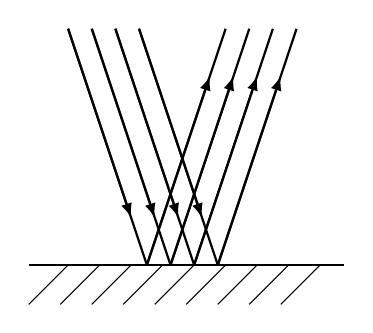
\begin{tikzpicture}
            \draw[thick] (-3, 0) -- (1, 0); % Ground line
            \foreach \i in {-3, -2.6, ..., 0.5} {
                \draw[] (\i, -0.5) -- (\i+0.5, 0); % Vertical lines
            }
            \foreach \i in {-2.5, -2.2, -1.9, -1.6} {
                \draw[thick, -latex] (\i, 3) -- (\i +0.8, 0.6);
                \draw[thick] (\i, 3) -- (\i+1, 0);
            }
            \foreach \i in {-2.5, -2.2, -1.9, -1.6} {
                \draw[thick, -latex] (\i+1, 0) -- (\i+1.8, 2.4);
                \draw[thick] (\i+1, 0) -- (\i+2, 3);
            }
        \end{tikzpicture}
        \caption{}
        \label{fig_chp1_reflection_1}
    \end{subfigure}
    \begin{subfigure}{.4\textwidth}
        \centering
        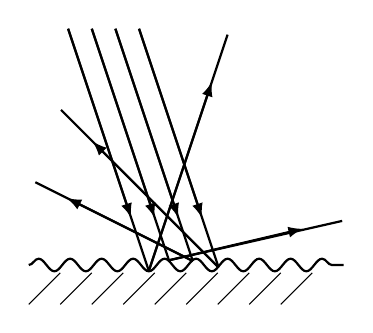
\begin{tikzpicture}
            \draw[thick,decorate,decoration={snake,amplitude=0.8mm,segment length=4mm}] (-3, 0) -- (1, 0); % Ground line
            \foreach \i in {-3, -2.6, ..., 0.5} {
                \draw[] (\i, -0.5) -- (\i+0.4, -0.1); % Vertical lines
            }

            \foreach \i in {-2.5, -2.2, -1.9, -1.6} {
                \draw[thick, -latex] (\i, 3) -- (\i +0.8, 0.6);
            }
            \draw[thick] (-2.5, 3) -- (-2.5+1+0.025, 0-0.075);
            \draw[thick, -latex] (-2.5+1+0.025, 0-0.075) -- (-2.5+1+0.025+0.8, 0-0.075+2.4);
            \draw[thick] (-2.5+1+0.025, 0-0.075) -- (-2.5+1+0.025+1, 0-0.075+3);

            \draw[thick] (-2.2, 3) -- (-2.2+1-0.02, 0+0.06);
            \draw[thick] (-2.2+1-0.02, 0+0.06) -- (-2.5+1-0.02+2.5, 0+0.06+0.5);
            \draw[thick, -latex] (-2.2+1-0.02, 0+0.06) -- (-2.5+1-0.02+2, 0+0.06+0.4);

            \draw[thick] (-1.9, 3) -- (-1.9+1-0.017, 0+0.051);
            \draw[thick] (-1.9+1-0.017, 0+0.051) -- (-1.9+1-0.017-2, 0+0.051+1);
            \draw[thick, -latex] (-1.9+1-0.017, 0+0.051) -- (-1.9+1-0.017-1.6, 0+0.051+0.8);

            \draw[thick] (-1.6, 3) -- (-1.6+1+0.01, 0-0.03);
            \draw[thick] (-1.6+1+0.01, 0-0.03) -- (-1.6+1+0.01-2, 0-0.03+2);
            \draw[thick, -latex] (-1.6+1+0.01, 0-0.03) -- (-1.6+1+0.01-1.6, 0-0.03+1.6);
        \end{tikzpicture}
        \caption{}
        \label{fig_chp1_reflection_2}
    \end{subfigure}
    \caption{电磁波的反射示意图 (a) 镜面反射 (b) 漫反射}
    \label{fig_chp1_reflection}
\end{figure}

不同的雷达系统会根据目标的反射特性选择合适的工作频率和波形。例如,气象雷达通常使用较低频率,以便更好地探测云层和降水;而军事雷达则可能使用更高频率,以提高分辨率和探测精度。

此外,隐身飞机为了降低被雷达探测的概率,通常会采用特殊的设计和材料来减少雷达波的反射。根据电磁波的反射特性,目前主流的隐身技术主要包括以下两种:
\begin{enumerate}
    \item \textbf{外形优化设计}:通过机身外形的精细设计,采用倾斜表面和尖锐棱角结构,尽可能避免出现直角和垂直面,以显著降低雷达波的直接反射。
    \item \textbf{结构与涂层设计}:飞机内部采用蜂窝状或多孔结构,以增强对雷达波的吸收;同时在机体表面涂覆特殊材料(如吸波材料或漫反射涂层),进一步降低雷达波的反射强度。
\end{enumerate}

利用镜面反射,还可以设计一种特殊的器械,叫作角反射器又名雷达反射器,简称角反。角反可以以将入射的电磁波反射回原方向,通常由三个互相垂直的平面组成,如\cref{fig_chp1_corner_reflector}所示。

\begin{figure}[htb!]
    \centering
    \begin{subfigure}{.3\textwidth}
        \centering
        \includegraphics[width=.8\textwidth]{./img/intro/corner_reflector_1.tikz}
        \caption{}
        \label{fig_chp1_corner_reflector_1}
    \end{subfigure}
    \begin{subfigure}{.3\textwidth}
        \centering
        \includegraphics[width=.9\textwidth]{./img/intro/corner_reflector_2.tikz}
        \caption{}
        \label{fig_chp1_corner_reflector_2}
    \end{subfigure}
    \caption{角反射器示意图 (a) 结构示意 (b) 工作原理}
    \label{fig_chp1_corner_reflector}
\end{figure}

事实上,角反在生活中非常常见。比如自行车的尾灯上通常会有一个小的角反射器(如\cref{fig_chp1_bike}所示),用于提高夜间行车的安全性。仔细观察可以发现,这种角反是由大量的小型角反组成的。

\begin{figure}[htb!]
    \centering
    
\includegraphics[width=.4\textwidth]{./img/intro/bike.jpeg}
    \caption{自行车尾部的角反射器}
    \label{fig_chp1_bike}
\end{figure}

由于角反可以有效地将入射的电磁波反射回原方向,因此可以提供稳定、明确的强回波信号,通常被用作雷达系统的校准目标,检验雷达设备的测距精度、方向精度和灵敏度。在航海与航空领域,角反射器常用于标识特定位置,如航道、海岸线或机场跑道周围,为雷达导航提供明确的位置标识,提高导航的准确性与安全性。

\subsection{电磁波的折射}

电磁波在不同介质中传播时,会发生折射现象。折射是指电磁波在穿过介质界面时,传播方向发生改变的现象。折射的程度取决于入射角和介质的折射率。折射率是描述介质对电磁波传播影响的一个重要参数,定义为电磁波在真空中的传播速度与光在该介质中的传播速度之比,即
\begin{equation}
    n = \frac{c}{v}.
    \label{eq:refraction_index}
\end{equation}

折射是一种常见现象,可以用斯涅尔定律(Snell's Law)来描述。斯涅尔定律表明,当电磁波从一种介质进入另一种介质时,入射角 $\theta_1$、折射角 $\theta_2$ 和两种介质的折射率 $n_1$、$n_2$ 之间满足以下关系:
\begin{equation}
    n_1 \sin \theta_1 = n_2 \sin \theta_2.
    \label{eq:snell_law}
\end{equation}

当电磁波以一个较大的入射角,从折射率较大的介质进入折射率较小的介质时,可能会出现
\[
    n_1 \sin \theta_1 > n_2,
\]
的情况。此时,即便是\( \theta_2 \) 达到 90°,也无法满足\cref{eq:snell_law},从而导致电磁波无法进入到低折射率介质中,而是全部反射回来。这种现象被称为全反射(Total Internal Reflection)。全反射的条件是入射角大于临界角 $\theta_c$,临界角可以通过以下公式计算:
\begin{equation}
    \sin \theta_c = \frac{n_2}{n_1}.
    \label{eq:critical_angle}
\end{equation}

光纤通信就是利用全反射原理实现的。光纤的核心部分具有较高的折射率,而包裹在外面的包层则具有较低的折射率。当光线以适当的入射角进入光纤时,会发生全反射,从而使光信号在光纤中传播而不损失能量。

在雷达系统中,折射现象也会影响电磁波的传播路径。在海面附近,由于水汽蒸发,会导致近海面小范围内大气湿度随高度锐减,从而形成一个较强的折射率梯度。或是在地面附近,出现逆温层,此时在一个较小的高度范围内,温度随高度增加而迅速升高,同样也会形成一个较强的折射率梯度。

\begin{figure}[htb!]
    \centering
    \includegraphics[width=.7\textwidth]{./img/intro/atmosphere_duct.tikz}
    \caption{大气波导示意图}
    \label{fig_chp1_atmosphere_duct}
\end{figure}

如\cref{fig_chp1_atmosphere_duct}所示,此时,电磁波在传播时,由于折射率梯度的存在,传播曲线会发生弯曲,导向海面或地面,并被反射。反射后,电磁波的路径会再次发生弯曲,入射角逐渐增大,直到出现全反射现象,将电磁波再次反射回地面。重复这一过程,电磁波便可以在大气层中沿着地面或海面传播很远的距离,而不会明显衰减。这种现象被称为大气波导(Atmospheric Ducting),也称为大气波导效应。除此以外,大气波导也可能发生在海拔数十米或数百米的空中,基本原理与上述类似,不再赘述。需要注意的是,\cref{fig_chp1_atmosphere_duct}仅为示意图,其中大气的折射率变化并不连续,仅为简化说明而作的分段近似。

当出现大气波导现象时,雷达可以探测到地平线以下的目标。尽管能够探测到目标,但却很难精确地测量目标的距离。如\cref{fig_chp1_radar_ducting}所示,由于大气波导效应,电磁波会沿着地表或海面传播,形成一个弯曲的路径,从而能够探测到地平线以下的目标。
\begin{figure}[htb!]
    \centering
    \includegraphics[width=.6\textwidth]{./img/intro/radar_atmosphere.tikz}
    \caption{雷达超视距探测示意图}
    \label{fig_chp1_radar_ducting}
\end{figure}

\subsection{自由空间路径损耗与大气衰减}

自由空间衰减(Free-Space Path Loss)则是指电磁波在自由空间中传播时,由于距离的增加而导致的功率损耗,通常被定义为发射功率与接收功率之间的比率。设有一个发射功率为 $P_t$ 的天线,以球面波形式向外辐射电磁波,则在距离 $r$ 处该电磁波的功率密度 $S$ 可以表示为:
\begin{equation*}
    S = \frac{P_t}{4 \pi r^2}.
    \label{eq:free_space_power_density}
\end{equation*}
而在此处的接收天线接收到的功率 $P_r$ 则与天线的有效面积 $A_e$ 有关,通常可以表示为:
\begin{equation*}
    P_r = S A_e = \frac{P_t A_e}{4 \pi r^2}.
    \label{eq:free_space_received_power}
\end{equation*}
其中,$A_e$ 是接收天线的有效面积,对于一个各向增益都为1的理想天线,其有效面积可以表示为:
\begin{equation*}
    A_e = \frac{\lambda^2}{4 \pi},
    \label{eq:effective_area}
\end{equation*}
其中 $\lambda$ 是电磁波的波长。
将\cref{eq:effective_area}代入\cref{eq:free_space_received_power},可以得到接收功率与发射功率之间的关系:
\begin{equation}
    L = \frac{P_t}{P_r} = \left( \frac{4 \pi r}{\lambda} \right)^2 = \left( \frac{4 \pi f r}{c} \right)^2.
    \label{eq:free_space_received_power_final}
\end{equation}
其中,$L$ 即为自由空间路径损耗。

从\cref{eq:free_space_received_power_final}可以看出,自由空间路径损耗与频率 $f$ 的平方成正比。所以想要进行远距离的探测,通常需要使用低频段的电磁波。但低频段的电磁波分辨率较低,无法提供足够的细节信息。因此,在自动驾驶、无人机等应用中,通常会使用高频的毫米波雷达(如24GHz或77GHz),以获得更高的分辨率和精度。

除此以外,电磁波在大气中传播时还会受到大气衰减的影响。大气衰减是指电磁波在大气中传播时,由于大气中的水汽、氧气、二氧化碳等分子对电磁波的吸收和散射\footnote{散射是指当波遇到空间中物体或介质的不均匀性(如界面、粗糙表面、微粒)时,入射波被扰动,产生新的传播方向和能量分布,从而向多方向重新辐射或传播的物理过程。在广义的波动物理概念中,散射包含了反射和折射引发的辐射场。}作用,导致信号强度的衰减。需要注意的是,大气衰减是指相对于自由空间路径损耗的大气导致的额外功率损耗。大气衰减与频率有关,通常在高频段(如微波和毫米波)更为显著。如\cref{fig_chp1_gaspl}所示,随着频率的增加,大气衰减会显著增加,并且湿空气的衰减比干燥空气更为明显。

\begin{figure}[htb!]
    \centering
    \includegraphics[width=.5\textwidth]{./img/intro/gaspl.tikz}
    \caption{大气衰减曲线\supercite{itu_r_p676_11}(距离1千米,温度$15^\circ$C,气压 $1013$ hPa)}
    \label{fig_chp1_gaspl}
\end{figure}

严格来说,大气本身只能对电磁波产生吸收或散射作用,能量并不会凭空增加。然而,从\cref{fig_chp1_gaspl}可以观察到,衰减数值在某些情况下可能为负值。也就是说,相对于在自由空间中传播,此时电磁波在大气中传播反而损耗更小。这主要是因为,在大气(尤其是近地层)中,温度、湿度等因素引起的折射率梯度会导致电磁波沿地表被导引传播,类似于波导效应,使得能量分布更加集中。因此,即便在较远的距离处,也能够接收到较强的信号。

\subsection{色散现象与多径效应}
电磁波在大气中传播除了会产生传输损耗(衰减)之外,还可能会产生失真。一般来说,产生失真的原因有两个,介质的色散现象和随机多径传输导致的干涉效应。

对于同一个介质,不同频率的电磁波在该介质中的传播速度有可能是不同的。这就会导致在传播的过程中,雷达发射的信号波形产生畸变,这种现象称为色散现象(Dispersion)。色散现象的一个典型例子是光在玻璃中的传播。当白光通过棱镜时,不同波长的光会以不同的速度传播,从而导致光线分散成彩虹色谱。如果我们将传播介质看作是一个线性系统,那么该系统的频率响应是非线性相位的。而对于一个非线性相位的系统,其输出信号的波形相较于输入信号波形会发生畸变。
\begin{figure}[htb!]
    \centering
    \begin{subfigure}{.3\textwidth}
        \centering
        \includegraphics[width=.9\textwidth]{./img/intro/filter1.tikz}
        \includegraphics[width=.9\textwidth]{./img/intro/filter4.tikz}
        \caption{}
        \label{fig_chp1_filter_1}
    \end{subfigure}
    \begin{subfigure}{.3\textwidth}
        \centering
        \includegraphics[width=.9\textwidth]{./img/intro/filter2.tikz}
        \includegraphics[width=.9\textwidth]{./img/intro/filter4.tikz}
        \caption{}
        \label{fig_chp1_filter_2}
    \end{subfigure}
    \begin{subfigure}{.3\textwidth}
        \centering
        \includegraphics[width=.9\textwidth]{./img/intro/filter3.tikz}
        \includegraphics[width=.9\textwidth]{./img/intro/filter4.tikz}
        \caption{}
        \label{fig_chp1_filter_3}
    \end{subfigure}
    \caption{色散现象示意图 (a) 原始信号及频谱 (b) 无色散滤波器输出 (c) 有色散滤波器输出}
    \label{fig_chp1_filter}
\end{figure}

如\cref{fig_chp1_filter}所示,可以看到,对于一个全通滤波器,如果相位响应是线性的,那么输出信号的波形与输入信号的波形相同,仅存在时延;反之,如果滤波器的相位响应是非线性的,那么输出信号的波形会发生畸变,但频谱仍然保持不变。不过大气对常见的雷达工作频率的色散效应并不明显,通常可以忽略不计。比如最靠近地表的对流层,其对20GHz以下的电磁波基本上是无色散的。

此外,多径效应(Multipath Effect),则是指电磁波在传播过程中,由于遇到障碍物或地形的反射、折射和散射等作用,导致同一信号在不同路径上到达接收天线的现象,如\cref{fig_chp1_multipath}所示。多径效应会导致接收信号的相位和幅度发生变化,从而引起信号的干扰和失真。严重时,不同路径上的信号可能会相互抵消,导致接收信号的强度显著降低。

\begin{figure}[htb!]
    \centering
    \includegraphics[width=.5\textwidth]{./img/intro/multipath.tikz}
    \caption{多径效应示意图}
    \label{fig_chp1_multipath}
\end{figure}

\section{雷达方程}
雷达方程(Radar Equation)是雷达系统最核心的工程公式之一,用于定量描述雷达发射、传播、反射和接收信号之间的功率关系。它既揭示了影响探测距离和信号强度的主要物理量,也为雷达系统设计提供了基础依据。本节已最简单的单站雷达(即发射接收天线距离很近,甚至共用同一个天线)为例,详细介绍雷达方程的推导过程。

设雷达系统的发射功率为 $P_t$,且发射天线增益为 $G_t$,那么在距离 $r$ 处的功率密度 $S$ 可以表示为:
\begin{equation*}
    S_t = \frac{P_t G_t}{4 \pi r^2}.
    \label{eq:radar_power_density}
\end{equation*}

而在此处的目标会将雷达发射的电磁波,以镜面反射、漫反射、体散射等方式反回给雷达接收天线,方便起见这里统称散射。由于目标的结构和材料千差万别,很难直接计算目标的散射特性,但可以使用雷达截面积(Radar Cross-Section, RCS)来整体性地描述目标对雷达波的散射能力。简而言之,如果目标的雷达截面积为 $\sigma$,那么目标散射的电磁波的总功率 $P_s$ 可以表示为:
\begin{equation*}
    P_s = S_t \sigma.
    \label{eq:radar_received_power}
\end{equation*}
因此,在接收天线处目标散射回来的电磁波的功率密度 $S_r$ 可以表示为:
\begin{equation*}
    S_r = \frac{P_s}{4 \pi r^2} = \frac{P_t G_t \sigma}{(4 \pi r^2)^2}.
    \label{eq:radar_received_power_density}
\end{equation*}

若接收天线的增益为 $G_r$。根据天线增益和有效面积的关系,接收天线的有效面积 $A_e$ 可以表示为:
\begin{equation}
    A_e = \frac{G_r \lambda^2}{4 \pi}.
    \label{eq:radar_effective_area}
\end{equation}
将接收天线有效面积\( A_e \)与目标散射回来的电磁波的功率密度\( S_r \)相乘,便可以得到接收天线接收到的功率 $P_r$ 为:
\begin{equation*}
    P_r = A_e S_r  = \frac{G_r \lambda^2}{4 \pi} \cdot \frac{P_t G_t \sigma}{(4 \pi r^2)^2}.
    \label{eq:radar_received_power_final}
\end{equation*}
将\cref{eq:radar_received_power_final}整理后,可以得到雷达方程的标准形式:
\begin{equation}
    P_r = \frac{P_t G_t G_r \lambda^2 \sigma}{(4 \pi)^3 r^4}.
    \label{eq:radar_equation}
\end{equation}

假设雷达能够检测的最小接收功率为 $P_{\text{min}}$,则根据\cref{eq:radar_equation},可以得到雷达的最大探测距离 $r_{\text{max}}$ 为:
\begin{equation}
    r_{\text{max}} = \left( \frac{P_t G_t G_r \lambda^2 \sigma}{(4 \pi)^3 P_{\text{min}}} \right)^{1/4}.
    \label{eq:radar_max_range}
\end{equation}
从\cref{eq:radar_max_range}可以看出,雷达的最大探测距离与发射功率 $P_t$、天线增益 $G_t$、接收天线增益 $G_r$、发射信号波长 $\lambda$ 以及目标的雷达截面积 $\sigma$ 成正比,而与接收机的最小接收功率 $P_{\text{min}}$ 成反比。

雷达方程与自由空间损耗有着密切的联系:显然,电磁波经历了从雷达到目标再从目标到雷达这两步传播过程,其中经历了两次自由空间损耗。如果我们将目标也看作是一个天线,那么目标的雷达截面积 $\sigma$ 则对应了天线的有效面积。因此,根据\cref{eq:radar_effective_area},我们可以得到目标作为一个天线时的增益为
\[
    G_s =  \frac{4 \pi \sigma}{\lambda^2}.
\]
此时,我们可以将发射功率与接收功率的比值写为
\begin{equation}
    \frac{P_t}{P_r} = \frac{(4 \pi)^3 r^4}{G_t G_r \lambda^2 \sigma} =\frac{(4 \pi r)^4}{\lambda^4 G_t G_r G_s} = \frac{L^2}{G_t G_r G_s},
    \label{eq:radar_equation_gain}
\end{equation}
其中 $L$ 是自由空间路径损耗,表达式见\cref{eq:free_space_received_power_final}。

\begin{figure}[htb!]
    \centering
    % \includegraphics[width=.4\textwidth]{./img}
    \begin{tikzpicture}
        \begin{axis}[
                xlabel=$ x $, ylabel=$ y $,
                ticklabel style={font=\small},
                label style={font=\small},
                axis equal image,
                axis lines=none,
                legend cell align=left,
                legend style={
                    anchor=north east,
                    font=\tiny,
                    draw=none,
                    fill=none
                }
            ]
            \addplot graphics [xmin=-0.5, xmax=0.5, ymin=-0.5, ymax=0.5] {img/radar.png};
            \addplot graphics [xmin=2.5, xmax=3.5, ymin=0.5, ymax=1.5] {img/target.png};
            % light from radar to target and back
            \addplot[thick, -latex, c1] coordinates {(0.5, 0.3) (2.5, 0.9)} node[midway, above=3pt, black] {\tiny 自由空间损耗\( L \)};
            \addplot[thick, -latex, c2] coordinates {(2.5, 0.8) (0.5, 0.2)} node[midway, below=3pt, black] {\tiny 自由空间损耗\( L \)};
            \node at (axis cs:0, 0.5) [font=\tiny] {发射增益\( G_t \)};
            \node at (axis cs:0, -0.5) [font=\tiny] {接收增益\( G_r \)};
            \node at (axis cs:3, 0.5) [font=\tiny] {目标增益\( G_s \)};
        \end{axis}
    \end{tikzpicture}
    \caption{雷达方程与自由空间损耗}
    \label{fig_chp1_radar_equation_gain}
\end{figure}

如\cref{fig_chp1_radar_equation_gain}所示,\cref{eq:radar_equation_gain}有明确的物理意义:在雷达系统中,电磁波首先向外发射电磁波,到达目标处,功率的损耗为 $L$ 倍;然后目标将电磁波散射回来,再由接收天线接收,相同路径再走一遍,此时又损耗了 $L$ 倍。又因为,所使用的天线有增益,且目标也并不是一个理想的点目标。所以,整体的损耗并没有达到 $L^2$,而是需要再除以各个环节的增益 $G_t G_r G_s$。

\section{小结}

本章主要介绍了雷达及其相关的基本概念、组成原理与工作特性。首先,回顾了雷达的起源,阐述了雷达利用电磁波反射实现目标探测的基本思想,并简要介绍了赫兹实验证实电磁波存在的过程。随后,系统地讲解了现代雷达的基本组成及其工作流程,包括波形产生、发射、接收及信号处理等环节,重点分析了不同工作频率雷达的应用特点。在此基础上,进一步探讨了电磁波在传播过程中的几种典型物理现象:反射、折射、大气波导、色散以及多径效应,并说明了这些现象对雷达探测的影响。最后,推导了雷达方程,揭示了雷达系统中各个参数之间的关系,为后续章节的深入学习奠定了基础。通过本章的学习,读者应能初步理解雷达的工作原理及其在实际应用中的重要性,为后续章节的深入研究做好准备。
\chapter{矩阵方法基础}

\section{矩阵分解}
矩阵分解是线性代数中的一个重要概念,它将一个矩阵分解为多个简单的矩阵的乘积。常见的矩阵分解方法包括特征分解、奇异值分解、稀疏分解等。这些分解方法在数值计算、信号处理和机器学习等领域有着广泛的应用。

\subsection{特征分解}
特征分解(Eigenvalue Decomposition)是线性代数中的一个重要概念,对于一个方阵\( \mathbf{A} \in \mathbb{R}^{n \times n} \),其特征值和特征向量是满足以下方程的标量和向量:
\begin{equation}
    \mathbf{A} \bm{v} = \lambda \bm{v}.
\end{equation}
其中,\( \lambda \) 是特征值,非零向量\( \bm{v} \) 是对应的特征向量。

如果矩阵\( \mathbf{A} \)一共有\( n \)个线性无关的特征向量,构成如下的特征向量矩阵
\[
    \bm{v} =
    \begin{bmatrix}
        \bm{v}_1 & \bm{v}_2 & \cdots & \bm{v}_n
    \end{bmatrix},
\]
那么有
\begin{equation}
    \mathbf{A} \mathbf{V} = \mathbf{V} \mathbf{\Lambda},
    \label{eq:eigen-decomposition}
\end{equation}
其中\( \mathbf{\Lambda} \)是一个对角矩阵,其对角线上的元素为对应的特征值,即
\[
    \mathbf{\Lambda} =
    \begin{bmatrix}
        \lambda_1 & 0         & \cdots & 0         \\
        0         & \lambda_2 & \cdots & 0         \\
        \vdots    & \vdots    & \ddots & \vdots    \\
        0         & 0         & \cdots & \lambda_n
    \end{bmatrix}.
\]
对\cref{eq:eigen-decomposition}两边同时左乘\( \mathbf{V}^{-1} \),可以得到
\begin{equation}
    \mathbf{A} = \mathbf{V} \mathbf{\Lambda} \mathbf{V}^{-1}.
    \label{eq:eigen-decomposition-inverse}
\end{equation}
式\cref{eq:eigen-decomposition-inverse}就是矩阵的特征分解形式,而能够被分解的矩阵被称为可对角化矩阵。进一步地,对于对称矩阵,则有\cref{thm:symmetric-eigen-decomposition}所述的特征分解形式。

\begin{theorem}[对称矩阵的特征分解]\label{thm:symmetric-eigen-decomposition}
    如果矩阵\( \mathbf{A} \)是一个对称矩阵,则其特征向量构成的矩阵为正交矩阵,即满足
    \[
        \mathbf{V}^{\mathrm{T}} \mathbf{V} = \mathbf{I}.
    \]
    此时,矩阵有如下特征分解
    \[
        \mathbf{A} = \mathbf{V} \mathbf{\Lambda} \mathbf{V}^{\mathrm{T}}.
    \]
\end{theorem}
\begin{proof}
    设\( \mathbf{A} \)的特征值为\( \lambda_1, \lambda_2, \ldots, \lambda_n \),对应的特征向量为\( \bm{v}_1, \bm{v}_2, \ldots, \bm{v}_n \)。由于\( \mathbf{A} \)是对称矩阵,所以
    \[
        \mathbf{A} \bm{v}_i = \mathbf{A}^{\mathrm{T}} \bm{v}_i = \lambda_i \bm{v}_i
    \]
    显然,对于任意的\( i \neq j \),都有如下两个等式成立:
    \[
        \begin{split}
            \bm{v}_i^{\mathrm{T}} \mathbf{A} \bm{v}_j & =  \bm{v}_i^{\mathrm{T}} (\mathbf{A} \bm{v}_j)= \lambda_j \bm{v}_i^{\mathrm{T}} \bm{v}_j,                         \\
            \bm{v}_i^{\mathrm{T}} \mathbf{A} \bm{v}_j & = \left(\mathbf{A}^{\mathrm{T}} \bm{v}_i\right)^{\mathrm{T}} \bm{v}_j = \lambda_i \bm{v}_i^{\mathrm{T}} \bm{v}_j.
        \end{split}
    \]
    因此有
    \[
        \lambda_j \bm{v}_i^{\mathrm{T}} \bm{v}_j = \lambda_i \bm{v}_i^{\mathrm{T}} \bm{v}_j.
    \]
    当\( \lambda_i \neq \lambda_j \)时,\( \bm{v}_i^{\mathrm{T}} \bm{v}_j = 0 \),即特征向量正交。当\( \lambda_i = \lambda_j \)时,可以验证对于任意的\( \alpha, \beta \in \mathbb{C} \),以两者为系数线性组合得到的向量
    \[
        \bm{v} = \alpha \bm{v}_i + \beta \bm{v}_j,
    \]
    也是特征向量,对应的特征值仍然是\( \lambda_i = \lambda_j \)。也就是说,由\( \bm{v}_i \)和\( \bm{v}_j \)张成的平面上的任意向量都是特征向量。从这个平面上可以选出两个正交的特征向量\( \bm{v}_i' \)和\( \bm{v}_j' \),作为新的特征向量。这样,就可以确保所有的特征向量互相之间是正交的。如对所有特征向量都进行归一化,令其模长为一,则有特征向、量构成的矩阵满足
    \[
        \mathbf{V} \mathbf{V}^{\mathrm{T}} = \mathbf{I}.
    \]
\end{proof}

然而并不是所有的矩阵都可以进行特征分解,对于部分矩阵,其特征向量可能线性相关。此时,矩阵\( \mathbf{V} \)不可逆,因此无法得到特征分解。比如,下方的\( 2 \times 2 \)矩阵:
\[
    \mathbf{A} =
    \begin{bmatrix}
        1 & 1 \\
        0 & 1
    \end{bmatrix}.
\]
设其特征值为\( \lambda \),则有
\[
    \det(\mathbf{A} - \lambda \mathbf{I}) = \det\left(
    \begin{bmatrix}
            1 - \lambda & 1           \\
            0           & 1 - \lambda
        \end{bmatrix}\right) = (1 - \lambda)^2 = 0.
\]
因此,该矩阵的两个特征值都是1,对应的特征向量相同,都为
\[
    \bm{v} =
    \begin{bmatrix}
        1 \\
        0
    \end{bmatrix}.
\]
对于这样不可对角化的矩阵,一方面我们可以进行广义特征分解,将矩阵分解为若尔当标准型(Jordan form):
\begin{theorem}[广义特征分解] \label{thm:jordan-decomposition}
    对于任意的\( n \times n \)矩阵\( \mathbf{A} \),存在一个可逆矩阵\( \mathbf{P} \)和一个分块对角矩阵\( \mathbf{J} \),使得
    \[
        \mathbf{A} = \mathbf{P} \mathbf{J} \mathbf{P}^{-1}.
    \]
    分块对角矩阵\( \mathbf{J} \)有如下形式
    \[
        \mathbf{J} =
        \begin{bmatrix}
            J_1    & 0      & \cdots & 0      \\
            0      & J_2    & \cdots & 0      \\
            \vdots & \vdots & \ddots & \vdots \\
            0      & 0      & \cdots & J_k
        \end{bmatrix},
    \]
    其中每个\( J_i \)是一个若尔当块(Jordan block),其形式为
    \[
        J_i =
        \begin{bmatrix}
            \lambda_i & 1         & 0         & \cdots & 0         \\
            0         & \lambda_i & 1         & \cdots & 0         \\
            0         & 0         & \lambda_i & \ddots & 0         \\
            \vdots    & \vdots    & \vdots    & \ddots & 1         \\
            0         & 0         & 0         & \cdots & \lambda_i
        \end{bmatrix}.
    \]
\end{theorem}
考虑到本书中基本不涉及广义特征分解,这里不再给出\cref{thm:jordan-decomposition}证明。除了广义特征分解外,我们还可以使用其他的矩阵分解方法来处理不可对角化的矩阵,比如下一小节给出的奇异值分解。

\begin{example}
    设有三座城市,且这三座城市之间人口流动的情况可以用一个矩阵来表示:
    \[
        \mathbf{P} =
        \begin{bmatrix}
            0.5 & 0.2 & 0.1 \\
            0.3 & 0.5 & 0.4 \\
            0.2 & 0.3 & 0.5
        \end{bmatrix},
    \]
    其中,\( P_{ij} \)表示单位时间内,从城市\( j \)流入到城市\( i \)的人口比例。比如\( P_{11} = 0.5 \),表明经过单位时间,有50\%的人口仍然留在城市1,\( P_{12} = 0.3 \)表示第2个城市30\%的人口会流动到城市1。请求解以下问题:
    \begin{enumerate}
        \item 假设初始时刻,三个城市的人口都为1000人,请计算经过一个单位时间后,各个城市的人口分布情况。
        \item 请计算经过足够长的时间后,各个城市的人口分布情况。
    \end{enumerate}
\end{example}
\begin{solution}
    \begin{enumerate}
        \item 记初始时刻三个城市的人口数量为如下向量
              \[
                  \bm{x}_0 =
                  \begin{bmatrix}
                      1000 \\
                      1000 \\
                      1000
                  \end{bmatrix}.
              \]
              则经过一个单位时间后,各个城市的人口数量为
              \[
                  \bm{x}_1 = \mathbf{P} \bm{x}_0 =
                  \begin{bmatrix}
                      0.5 & 0.2 & 0.1 \\
                      0.3 & 0.5 & 0.4 \\
                      0.2 & 0.3 & 0.5
                  \end{bmatrix}
                  \begin{bmatrix}
                      1000 \\
                      1000 \\
                      1000
                  \end{bmatrix} =
                  \begin{bmatrix}
                      800  \\
                      1200 \\
                      1000
                  \end{bmatrix}.
              \]

        \item 设\( \bm{x}_n \)为经过\( n \)个单位时间后,各个城市的人口分布情况。则有
              \[
                  \bm{x}_n = \mathbf{P} \bm{x}_{n-1} = \mathbf{P}^n \bm{x}_0.
              \]
              又因为\( \mathbf{P} \)有如下特征分解
              \[
                  \mathbf{P} = \mathbf{V} \mathbf{\Lambda} \mathbf{V}^{-1},
              \]
              其中
              \[
                  \mathbf{V} \approx
                  \begin{bmatrix}
                      0.3995 & -0.8090 & 0.3090  \\
                      0.7068 & 0.3090  & -0.8090 \\
                      0.5839 & 0.5000  & 0.5000
                  \end{bmatrix}, \quad \mathbf{\Lambda} \approx
                  \begin{bmatrix}
                      1 & 0      & 0      \\
                      0 & 0.3618 & 0      \\
                      0 & 0      & 0.1382
                  \end{bmatrix}.
              \]
              因此,当\( n \)趋向于无穷大时,\( \mathbf{P}^n \)的极限为
              \[
                  \lim_{n \to \infty} \mathbf{P}^n = \lim_{n \to \infty} \mathbf{V} \mathbf{\Lambda}^n \mathbf{V}^{-1} = \mathbf{V}
                  \begin{bmatrix}
                      1 & 0 & 0 \\
                      0 & 0 & 0 \\
                      0 & 0 & 0
                  \end{bmatrix} \mathbf{V}^{-1} \approx
                  \begin{bmatrix}
                      0.2364 & 0.2364 & 0.2364 \\
                      0.4182 & 0.4182 & 0.4182 \\
                      0.3455 & 0.3455 & 0.3455
                  \end{bmatrix}.
              \]
              于是,经过足够长的时间后,各个城市的人口分布情况为
              \[
                  \bm{x}_\infty = \lim_{n \to \infty} \bm{x}_n = \lim_{n \to \infty} \mathbf{P}^n \bm{x}_0 \approx
                  \begin{bmatrix}
                      709.1  \\
                      1254.5 \\
                      1036.4
                  \end{bmatrix}.
              \]

    \end{enumerate}
\end{solution}

\subsection{奇异值分解}

奇异值分解(Singular Value Decomposition, SVD)是线性代数中一个非常重要的矩阵分解工具,被广泛应用于信号处理、统计学、机器学习、图像压缩等领域。

相比于特征分解,奇异值分解可以应用于任意形状的矩阵(包括非方阵),并且不要求矩阵是可逆的,见下方的定理。

\begin{theorem}
    对于任意的矩阵\( \mathbf{A} \in \mathbb{R}^{m \times n} \),都存在一个奇异值分解:
    \[
        \mathbf{A} = \mathbf{U} \mathbf{S} \mathbf{V}^{\mathrm{T}},
    \]
    其中,\( \mathbf{U} \in \mathbb{R}^{m \times m} \)是一个正交矩阵,\( \mathbf{V} \in \mathbb{R}^{n \times n} \)是一个正交矩阵,\( \mathbf{S} \in \mathbb{R}^{m \times n} \)是一个对角矩阵,对角线上的元素为\( \mathbf{A} \)的奇异值(singular values)。
\end{theorem}
\begin{proof}
    不妨假设\( m \geq n \),则\( \mathbf{A}^{\mathrm{T}} \mathbf{A} \) 为一个\( n \times n \)的对称矩阵。根据特征分解定理,存在一个正交矩阵\( \mathbf{V} \)和一个对角矩阵\( \mathbf{\Lambda} \),使得
    \[
        \mathbf{A}^{\mathrm{T}} \mathbf{A} = \mathbf{V} \mathbf{\Lambda} \mathbf{V}^{\mathrm{T}}.
    \]
    可以验证,\( \mathbf{\Lambda} \)的对角元素必然是非负的,因此不妨将矩阵\( \mathbf{A}^{\mathrm{T}} \mathbf{A} \)的特征值记作\( \lambda_i^2 \)。令\( \bm{v}_i \)为\( \mathbf{V} \)的第\( i \)列向量,并令
    \[
        \bm{u}_i = \frac{\mathbf{A} \bm{v}_i}{\|\mathbf{A} \bm{v}_i\|} = \frac{\mathbf{A} \bm{v}_i}{\sqrt{\bm{v}_i^{\mathrm{T}} \mathbf{A}^{\mathrm{T}} \mathbf{A} \bm{v}_i}} = \frac{1}{\lambda_i} \mathbf{A} \bm{v}_i.
    \]
    则有
    \[
        \bm{u}_i^{\mathrm{T}} \mathbf{A} \bm{v}_i = \frac{1}{\lambda_i} \bm{v}_i^{\mathrm{T}} \mathbf{A}^{\mathrm{T}} \mathbf{A} \bm{v}_i = \frac{1}{\lambda_i} \lambda_i^2 = \lambda_i.
    \]

    因此,可以构造如下的矩阵
    \[
        \mathbf{U} =
        \begin{bmatrix}
            \bm{u}_1 & \bm{u}_2 & \cdots & \bm{u}_n & \bm{u}_{n+1} & \cdots & \bm{u}_m
        \end{bmatrix} \in \mathbb{R}^{m \times m},
    \]
    对于其中的列向量,当\( 1 \leq i \leq n \)时,有\( \bm{u}_i = \frac{\mathbf{A} \bm{v}_i}{\|\mathbf{A} \bm{v}_i\|} \);而当\( n + 1 \leq i \leq m \)时,可以令\( \bm{u}_i \)为\( \mathbf{A} \)的零空间中的任意向量,只需满足构成的矩阵\( \mathbf{U} \)是一个正交矩阵即可。

    对于构造的矩阵\( \mathbf{U} \),可以验证其满足
    \[
        \mathbf{U}^{\mathrm{T}} \mathbf{A} \mathbf{V} =
        \begin{bmatrix}
            \sqrt{\mathbf{\Lambda}} \\
            \mathbf{0}
        \end{bmatrix} \in \mathbb{R}^{m \times n},
    \]
    其中\( \sqrt{\mathbf{\Lambda}} \)是\( \mathbf{\Lambda} \)的开平方,也是一个对角矩阵,其对角线上的元素为\( \lambda_i \),而\( \mathbf{0} \)是一个\( (m - n) \times n \)的全零矩阵。记该分块矩阵为\( \mathbf{S} \), 并对上式两边同时左乘\( \mathbf{U} \),右乘\( \mathbf{V}^{\mathrm{T}} \),即可得到
    \[
        \mathbf{A} = \mathbf{U} \mathbf{S} \mathbf{V}^{\mathrm{T}}.
    \]
\end{proof}

有意思的是,对于对称矩阵,其奇异值分解和特征分解是等价的。不妨设有对称矩阵\( \mathbf{A} \in \mathbb{R}^{n \times n} \),其SVD分解为
\[
    \mathbf{A} = \mathbf{U} \mathbf{S} \mathbf{V}^{\mathrm{T}}.
\]
又因为\( \mathbf{A}^{\mathrm{T}} = \mathbf{A} \),因此有
\[
    \mathbf{A} = \mathbf{A}^{\mathrm{T}}= \left( \mathbf{U} \mathbf{S} \mathbf{V}^{\mathrm{T}} \right)^{\mathrm{T}} = \mathbf{V} \mathbf{S}^{\mathrm{T}} \mathbf{U}^{\mathrm{T}}.
\]
注意到\( \mathbf{S} \) 是一个\( n \times n \)的对角矩阵,所以\( \mathbf{S}^{\mathrm{T}}  = \mathbf{S} \),至此可以得到如下等式
\[
    \mathbf{A} = \mathbf{U} \mathbf{S} \mathbf{V}^{\mathrm{T}} = \mathbf{V} \mathbf{S} \mathbf{U}^{\mathrm{T}}.
\]
观察上式,不难发现\( \mathbf{U} =  \mathbf{V} \)。此时,对称矩阵\( \mathbf{A} \)的特征分解可以写为\( \mathbf{A} = \mathbf{V} \mathbf{S} \mathbf{V}^{\mathrm{T}} \),因此对称矩阵的奇异值分解和特征分解是等价的。

除此以外,SVD分解实际上提供了一种对矩阵进行低秩近似的方法。考虑如下优化问题:
\begin{equation}
    \begin{cases}
        \min_{\mathbf{B}} & \|\mathbf{A} - \mathbf{B}\|_{\mathrm{F}}^2 \\
        \text{s.t}        & \text{rank}(\mathbf{B}) = k
    \end{cases}
    \label{eq:sparse-approximation}
\end{equation}
其中\( \|\cdot\|_F \)表示矩阵的Frobenius范数。通过计算\( \mathbf{A} \)的SVD分解,并保留最大的\( k \)个奇异值和对应的奇异向量,可以该优化问题的最优解:
\begin{equation}
    \mathbf{B} = \sum_{i=1}^{k} \lambda_i \bm{u}_i \bm{v}_i^{\mathrm{T}},
    \label{eq:sparse-approximation-solution}
\end{equation}
其中\( \lambda_i \)是矩阵\( \mathbf{A} \)第\( i \)大的奇异值。具体证明不再展开,请读者自行推导。

\begin{example}
    对于如\cref{fig_singular_values}所示的灰度图像,可以将其看作是一个\( 200 \times 300 \)的矩阵,请利用奇异值分解对其进行压缩处理。
    \begin{figure}[htb!]
        \centering
        
\includegraphics[width=.3\textwidth]{./img/matrix/cat_resized.jpg}
        \caption{原始灰度图像}
        \label{fig_cat_gray}
    \end{figure}
\end{example}
\begin{solution}
    直接对图像矩阵进行奇异值分解,得到
    \[
        \mathbf{A} = \mathbf{U} \mathbf{S} \mathbf{V}^{\mathrm{T}}.
    \]
    其中\( \mathbf{S} \)的对角线元素从大到小排列绘制的曲线如\cref{fig_singular_values}所示。从图中可以看到,奇异值数值大小从大到小迅速下降,这表明大部分信息都集中在较大的奇异值对应的特征向量上。
    \begin{figure}[htb!]
        \centering
        \includegraphics[width=.6\textwidth]{./img/matrix/cat_svd.tikz}
        \caption{奇异值大小分布}
        \label{fig_singular_values}
    \end{figure}

    因此,我们可以通过保留前\( k \)个奇异值来实现图像的压缩。具体而言,设\( k \)为保留的奇异值个数,则压缩后的图像矩阵为原始矩阵的低秩近似:
    \[
        \mathbf{A}_{\text{compressed}} = \mathbf{U}_{k} \mathbf{S}_{k} \mathbf{V}_{k}^{\mathrm{T}},
    \]
    其中\( \mathbf{U}_k \in \mathbb{R}^{m \times k} \)是\( \mathbf{U} \)的前\( k \)列,\( \mathbf{S}_k \in \mathbb{R}^{k \times k} \)是\( \mathbf{S} \)的前\( k \)行和前\( k \)列,\( \mathbf{V}_k \in \mathbb{R}^{n \times k} \)是\( \mathbf{V} \)的前\( k \)列。

    通过调整\( k \)的值,可以控制压缩后的图像质量和文件大小,如\cref{fig_compressed_images}所示。可以看到,随着\( k \)的增大,图像质量逐渐提高,当\( k=50 \)时,图像质量已经非常接近原始图像,此时,对应的三个矩阵的元素个数大约只有原始矩阵元素个数的41\%。
    \begin{figure}[htb!]
        \centering
        \begin{subfigure}{.3\textwidth}
            \centering
            
\includegraphics[width=.9\textwidth]{./img/matrix/cat_approx1.jpg}
            \caption{}
            \label{fig_compressed_images_1}
        \end{subfigure}
        \begin{subfigure}{.3\textwidth}
            \centering
            
\includegraphics[width=.9\textwidth]{./img/matrix/cat_approx2.jpg}
            \caption{}
            \label{fig_compressed_images_2}
        \end{subfigure}
        \begin{subfigure}{.3\textwidth}
            \centering
            
\includegraphics[width=.9\textwidth]{./img/matrix/cat_approx3.jpg}
            \caption{}
            \label{fig_compressed_images_3}
        \end{subfigure}
        \caption{奇异值分解压缩后的图像 (a) \( k = 10 \) (b) \( k = 20 \) (c) \( k = 50 \)}
        \label{fig_compressed_images}
    \end{figure}
\end{solution}

\subsection{稀疏分解}
稀疏分解(Sparse Decomposition)是指将一个观测向量表示为一个字典矩阵与一个稀疏系数向量的乘积。该方法在信号处理、图像处理和机器学习等领域具有广泛应用,尤其在特征提取、压缩编码和降维等任务中表现出强大的建模能力。

稀疏分解对应的优化问题可以表示为
\begin{equation}
    \begin{cases}
        \min_{\bm{x}} & \left\| \bm{x} \right\|_0  \\
        \text{s.t}    & \mathbf{D} \bm{x} = \bm{y}
    \end{cases},
    \label{eq:sparse-decomposition}
\end{equation}
其中,\( \bm{y} \in \mathbb{R}^m \)是观测向量,\( \mathbf{D} \in \mathbb{R}^{m \times n} \)是字典矩阵。一般来说,\( n \gg m \),这意味着方程\( \mathbf{D} \bm{x} = \bm{y} \)可能有多个甚至无穷多个解。而稀疏分解则是希望找到其中最稀疏的那个解,即使得系数向量\( \bm{x} \)的非零元素个数最少。当存在噪声时,等式\( \mathbf{D} \bm{x} = \bm{y} \)可能无法完全满足,此时可以将约束条件改为
\begin{equation}
    \begin{cases}
        \min_{\bm{x}} & \left\| \bm{x} \right\|_0                                     \\
        \text{s.t}    & \left\| \bm{y} - \mathbf{D} \bm{x} \right\|_2 \leq \epsilon^2
    \end{cases}.
    \label{eq:sparse-decomposition-noisy}
\end{equation}

然而,优化问题 \cref{eq:sparse-decomposition} 中的 \( \ell_0 \)-范数是非凸且不连续的,使得该问题属于 NP-hard 问题,难以直接求解。因此,通常采用以下近似方法进行求解:

\begin{enumerate}[label=\arabic*.]
    \item \textbf{基追踪(Basis Pursuit, BP)}:将 \( \ell_0 \)-范数替换为其凸包 \( \ell_1 \)-范数,转化为如下凸优化问题:
          \begin{equation}
              \begin{cases}
                  \min_{\bm{x}} \quad & \left\| \bm{x} \right\|_1                                                                          \\
                  \text{s.t.} \quad   & \mathbf{D} \bm{x} = \bm{y} \text{ 或 } \left\| \bm{y} - \mathbf{D} \bm{x} \right\|_2 \leq \epsilon.
              \end{cases}
              \label{eq:basis-pursuit}
          \end{equation}
          在满足一定条件,如限制性等距条件(Restricted Isometry Property)时,该方法能够准确恢复原始的稀疏解。并且,可以通过成熟的线性规划(Linear Programming)或二阶锥规划(Second-Order Cone Programming)等算法高效求解。

    \item \textbf{LASSO(Least Absolute Shrinkage and Selection Operator)}:通过引入 \( \ell_1 \)-范数正则项,构造如下优化模型:
          \begin{equation}
              \min_{\bm{x} \in \mathbb{R}^n} \left\| \bm{y} - \mathbf{D} \bm{x} \right\|_2^2 + \lambda \left\| \bm{x} \right\|_1,
              \label{eq:lasso}
          \end{equation}
          其中,\( \lambda > 0 \) 是正则化参数,用于权衡数据拟合精度与解的稀疏性。LASSO 更适用于存在观测噪声的实际应用场景,可以通过坐标下降法(Coordinate Descent)、交替方向乘子法(Alternating Direction Method of Multipliers, ADMM)等算法高效求解。
\end{enumerate}

除了上述方法,稀疏分解还可以采用匹配追踪(Matching Pursuit)、正交匹配追踪(Orthogonal Matching Pursuit, OMP)、迭代阈值法(Iterative Thresholding)等方法进行求解,这些方法在计算效率和精度之间提供了不同的折中选择。

将稀疏分解拓展到矩阵的情形,可以得到\( k \)-SVD(\( k \)-Sparse Singular Value Decomposition)模型。该模型假设矩阵的奇异值分解可以表示为一个稀疏系数向量与字典矩阵的乘积。具体而言,给定一个矩阵 \( \mathbf{Y} \in \mathbb{R}^{m \times n} \),对应的 \( k \)-SVD 优化问题可以表示为
\begin{equation}
    \begin{cases}
        \min_{\mathbf{D}, \mathbf{X}} & \left\| \mathbf{Y} - \mathbf{D} \mathbf{X} \right\|_{\mathrm{F}}^2 \\
        \text{s.t.}                   & \left\| \bm{x}_i \right\|_0 = 1, \quad \forall i = 1, \ldots, n
    \end{cases},
    \label{eq:k-svd}
\end{equation}
其中,\( \mathbf{D} \in \mathbb{R}^{m \times k} \)是字典矩阵,\( \mathbf{X} =
\begin{bsmallmatrix} \bm{x}_1 & \bm{x}_2 & \cdots & \bm{x}_n
\end{bsmallmatrix} \in \mathbb{R}^{k \times n} \)是稀疏系数矩阵。\( k \)-SVD是对聚类算法\( k \)-均值(\( k \)-Means)的一种推广,其中字典矩阵的列向量对应聚类中心,而稀疏系数矩阵\( \mathbf{X} \)则包含了聚类结果。

除此以外,稀疏分解的矩阵推广还有另一种形式,即鲁棒主成分分析(Robust Principal Component Analysis, RPCA)。RPCA假设观测矩阵可以分解为一个低秩矩阵和一个稀疏矩阵的和。具体而言,给定一个矩阵 \( \mathbf{Y} \in \mathbb{R}^{m \times n} \),RPCA 的优化问题可以表示为
\begin{equation}
    \begin{cases}
        \min_{\mathbf{L}, \mathbf{S}} & \left\| \mathbf{L} \right\|_* + \lambda \left\| \operatorname{vec}(\mathbf{S})\right\|_1 \\
        \text{s.t.}                   & \mathbf{Y} = \mathbf{L} + \mathbf{S}
    \end{cases},
    \label{eq:rpca}
\end{equation}
其中,\( \mathbf{L} \in \mathbb{R}^{m \times n} \)是低秩矩阵,\( \left\| \cdot \right\|_* \)表示核范数,\( \mathbf{S} \in \mathbb{R}^{m \times n} \)是稀疏矩阵,\( \left\| \operatorname{vec}(\cdot)\right\|_1 \)表示将矩阵展开为向量后的 \( \ell_1 \)-范数,也即矩阵所有元素的绝对值之和。由于稀疏项的存在,RPCA能够有效提取数据中的异常,同时保留主要的低秩结构。

\begin{example}
    请对如\cref{fig_rpca_example}所示的包含椒盐噪声的图像矩阵进行去噪处理。
    \begin{figure}[htb!]
        \centering
        
\includegraphics[width=.3\textwidth]{./img/matrix/cat_noisy.jpg}
        \caption{包含椒盐噪声的图像}
        \label{fig_rpca_example}
    \end{figure}
\end{example}
\begin{solution}
    不难发现,椒盐噪声对应的矩阵是一个稀疏矩阵,而原始图像矩阵则是一个低秩矩阵。因此,我们可以使用鲁棒主成分分析(RPCA)来对其进行去噪处理。算法结果如\cref{fig_rpca_result}所示,可以看到,所分离出的低秩矩阵基本对应无噪声的图像,而稀疏矩阵则对应椒盐噪声部分。
    \begin{figure}[htb!]
        \centering
        \begin{subfigure}{.3\textwidth}
            \centering
            
\includegraphics[width=.9\textwidth]{./img/matrix/cat_low_rank.jpg}
            \caption{}
            \label{fig_rpca_result_1}
        \end{subfigure}
        \begin{subfigure}{.3\textwidth}
            \centering
            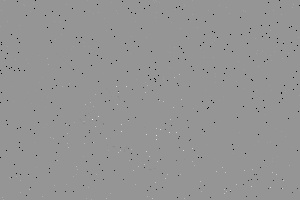
\includegraphics[width=.9\textwidth]{./img/matrix/cat_sparse.jpg}
            \caption{}
            \label{fig_rpca_result_2}
        \end{subfigure}
        \caption{鲁棒主成分分析结果 (a) 低秩矩阵 (b) 稀疏矩阵}
        \label{fig_rpca_result}
    \end{figure}
\end{solution}

\section{矩阵微分}

\subsection{实矩阵微分}
普通的求导想必大家都很熟悉,比如对于标量函数$f(x)$, 其关于$x$的导数可以表示为\( \frac{\partial f(x)}{\partial x} \)。 而函数不仅仅可以是关于标量的函数,也可以是关于向量甚至矩阵的函数。比如,一个二元函数\( f(x_1, x_2) \)则可以看作是关于向量\( \bm{x} = \begin{bsmallmatrix} x_1 & x_2 \end{bsmallmatrix}^{\mathrm{T}} \)的一个函数\( f(\bm{x}) \)。自然地,我们也可以求解其关于向量\( \bm{x} \)导数。具体而言,我们有如下定义。

\begin{definition}[标量关于向量求导]
    对于向量$\bm{x} \in \mathbb{R}^{n \times 1}$,有映射\( f: \mathbb{R}^{n \times 1} \rightarrow \mathbb{R} \),则定义其关于向量\( \bm{x} \)导数为
    \[
        \frac{\partial f(\bm{x})}{\partial \bm{x}}  =
        \begin{bmatrix}
            \frac{\partial f(\bm{x})}{\partial x_1} \\
            \frac{\partial f(\bm{x})}{\partial x_2} \\
            \vdots                                  \\
            \frac{\partial f(\bm{x})}{\partial x_n}
        \end{bmatrix}.
    \]
\end{definition}

换句话说,\( f(\bm{x}) \)关于\( \bm{x} \)导数可以通过计算\( f(\bm{x}) \)关于\( \bm{x} \)中每一个元素的偏导数,并将结果排列成和\( \bm{x} \)同样维度的向量。类似地,我们也可以定义标量对矩阵的求导,具体定义如下。

\begin{definition}[标量关于矩阵求导]
    对于矩阵$\mathbf{A} \in \mathbb{R}^{m \times n}$,有映射\( f: \mathbb{R}^{m \times n} \rightarrow \mathbb{R} \),则定义其关于矩阵\( \mathbf{A} \)导数为
    \[
        \frac{\partial f(\mathbf{A})}{\partial \mathbf{A}} =
        \begin{bmatrix}
            \frac{\partial f(\mathbf{A})}{\partial a_{11}} & \frac{\partial f(\mathbf{A})}{\partial a_{12}} & \cdots & \frac{\partial f(\mathbf{A})}{\partial a_{1n}} \\
            \frac{\partial f(\mathbf{A})}{\partial a_{21}} & \frac{\partial f(\mathbf{A})}{\partial a_{22}} & \cdots & \frac{\partial f(\mathbf{A})}{\partial a_{2n}} \\
            \vdots                                         & \vdots                                         & \ddots & \vdots                                         \\
            \frac{\partial f(\mathbf{A})}{\partial a_{m1}} & \frac{\partial f(\mathbf{A})}{\partial a_{m2}} & \cdots & \frac{\partial f(\mathbf{A})}{\partial a_{mn}}
        \end{bmatrix}.
    \]
\end{definition}

此外,函数本身也有可能不是一个标量,而是一个向量,因此我们也需要定义向量对向量的求导。具体定义如下:

\begin{definition}[向量关于向量求导]
    对于向量\( \bm{x} \in \mathbb{R}^{m \times 1} \),有映射\( \bm{f}: \mathbb{R}^{n \times 1} \rightarrow \mathbb{R}^{m \times 1} \),则定义其关于向量\( \bm{x} \)导数为
    \[
        \frac{\partial \bm{f}(\bm{x})}{\partial \bm{x}} =
        \begin{bmatrix}
            \frac{\partial f_1(\bm{x})}{\partial \bm{x}} \\
            \frac{\partial f_2(\bm{x})}{\partial \bm{x}} \\
            \vdots                                       \\
            \frac{\partial f_m(\bm{x})}{\partial \bm{x}}
        \end{bmatrix}.
    \]
\end{definition}
可以看到,对应的求导规则就是将函数的每一个元素分别对向量\( \bm{x} \)求导,并将结果按照\( \bm{f} \)的形式排列。比如,\( m \times 1 \)列向量关于\( n \times 1 \)列向量的导数为一个\( mn \times 1 \)的列向量。如果是\( 1 \times m \)的行向量关于\( n \times 1 \)列向量的导数,那么根据规则,结果则是一个\( n \times m \)的矩阵。

接下来,本节给出一些常见的矩阵微分公式,这些公式在本书的后续章节中会经常用到。

\begin{example}
    设有向量\( \bm{x} \in \mathbb{R}^{n \times 1} \)、\( \bm{y} \in \mathbb{R}^{n \times 1} \) 和矩阵\( \mathbf{A} \in \mathbb{R}^{n \times n} \),计算如下导数
    \begin{enumerate}
        \item \( f = \bm{x}^{\mathrm{T}} \bm{y} \) 关于\( \bm{x} \)的导数
        \item \( f = \bm{x}^{\mathrm{T}} \bm{y} \) 关于\( \bm{y} \)的导数
        \item \( f = \bm{x}^{\mathrm{T}} \mathbf{A} \bm{y} \) 关于\( \bm{x} \)的导数
        \item \( f = \bm{x}^{\mathrm{T}} \mathbf{A} \bm{y} \) 关于\( \mathbf{A} \)的导数
        \item \( \bm{f} = \bm{x}^{\mathrm{T}} \mathbf{A} \) 关于\( \bm{x} \)的导数
        \item \( \bm{f} = (\bm{x} - \bm{y})^{\mathrm{T}} \) 关于\( \bm{x} \)的导数
    \end{enumerate}
\end{example}
\begin{solution}
    \begin{enumerate}
        \item 注意到\( f = \bm{x}^{\mathrm{T}} \bm{y}  = \sum_{i=1}^{n} x_i y_i\),因此有
              \[
                  \frac{\partial f}{\partial \bm{x}} =
                  \begin{bmatrix}
                      \frac{\partial f}{\partial x_1} \\
                      \frac{\partial f}{\partial x_2} \\
                      \vdots                          \\
                      \frac{\partial f}{\partial x_n}
                  \end{bmatrix} =
                  \begin{bmatrix}
                      y_1    \\
                      y_2    \\
                      \vdots \\
                      y_n
                  \end{bmatrix} = \bm{y}.
              \]
        \item 同理,对于\( f = \bm{x}^{\mathrm{T}} \bm{y}  \)有
              \[
                  \frac{\partial f}{\partial \bm{y}} =
                  \begin{bmatrix}
                      \frac{\partial f}{\partial y_1} \\
                      \frac{\partial f}{\partial y_2} \\
                      \vdots                          \\
                      \frac{\partial f}{\partial y_n}
                  \end{bmatrix} =
                  \begin{bmatrix}
                      x_1    \\
                      x_2    \\
                      \vdots \\
                      x_n
                  \end{bmatrix} = \bm{x}.
              \]
        \item 同样地,将函数写成求和的形式\( f = \bm{x}^{\mathrm{T}} \mathbf{A} \bm{y} = \sum_{i=1}^{n} \sum_{j=1}^{n} a_{ij} x_i  y_j \),因此有
              \[
                  \frac{\partial f}{\partial \bm{x}} =
                  \begin{bmatrix}
                      \frac{\partial f}{\partial x_1} \\
                      \frac{\partial f}{\partial x_2} \\
                      \vdots                          \\
                      \frac{\partial f}{\partial x_n}
                  \end{bmatrix} =
                  \begin{bmatrix}
                      \sum_{j=1}^{n} a_{1j} y_j \\
                      \sum_{j=1}^{n} a_{2j} y_j \\
                      \vdots                    \\
                      \sum_{j=1}^{n} a_{nj} y_j
                  \end{bmatrix} = \mathbf{A} \bm{y}.
              \]
        \item 同理,对于\( f = \bm{x}^{\mathrm{T}} \mathbf{A} \bm{y} \)有
              \[
                  \frac{\partial f}{\partial \mathbf{A}} =
                  \begin{bmatrix}
                      \frac{\partial f}{\partial a_{11}} & \frac{\partial f}{\partial a_{12}} & \cdots & \frac{\partial f}{\partial a_{1n}} \\
                      \frac{\partial f}{\partial a_{21}} & \frac{\partial f}{\partial a_{22}} & \cdots & \frac{\partial f}{\partial a_{2n}} \\
                      \vdots                             & \vdots                             & \ddots & \vdots                             \\
                      \frac{\partial f}{\partial a_{n1}} & \frac{\partial f}{\partial a_{n2}} & \cdots & \frac{\partial f}{\partial a_{nn}}
                  \end{bmatrix} =
                  \begin{bmatrix}
                      x_1 y_1 & x_1 y_2 & \cdots & x_1 y_n \\
                      x_2 y_1 & x_2 y_2 & \cdots & x_2 y_n \\
                      \vdots  & \vdots  & \ddots & \vdots  \\
                      x_n y_1 & x_n y_2 & \cdots & x_n y_n
                  \end{bmatrix} = \bm{x} \bm{y}^{\mathrm{T}}.
              \]
        \item 最后,对于\( \bm{f} = \bm{x}^{\mathrm{T}} \mathbf{A} \),其第\( j \)个元素为\( f_j = \sum_{i=1}^{n} a_{ij} x_i \),因此有
              \[
                  \frac{\partial f}{\partial \bm{x}} =
                  \begin{bmatrix}
                      \frac{\partial f_1}{\partial \bm{x}} & \frac{\partial f_2}{\partial \bm{x}} & \cdots & \frac{\partial f_n}{\partial \bm{x}}
                  \end{bmatrix} =
                  \begin{bmatrix}
                      a_{11} & a_{12} & \cdots & a_{1n} \\
                      a_{21} & a_{22} & \cdots & a_{2n} \\
                      \vdots & \vdots & \ddots & \vdots \\
                      a_{n1} & a_{n2} & \cdots & a_{nn}
                  \end{bmatrix} = \mathbf{A}.
              \]
        \item 对于\( \bm{f} = \bm{x} - \bm{y} \),有
              \[
                  \frac{\partial \bm{f}}{\partial \bm{x}} =
                  \begin{bmatrix}
                      \frac{\partial (x_1 - y_1)}{\partial \bm{x}} & \frac{\partial (x_2 - y_2)}{\partial \bm{x}} & \cdots & \frac{\partial (x_n - y_n)}{\partial \bm{x}}
                  \end{bmatrix} =
                  \begin{bmatrix}
                      1      & 0      & \cdots & 0      \\
                      0      & 1      & \cdots & 0      \\
                      \vdots & \vdots & \ddots & \vdots \\
                      0      & 0      & \cdots & 1
                  \end{bmatrix} = \mathbf{I}.
              \]
    \end{enumerate}
\end{solution}

从上面的例子中,我们可以得到一些经验结论:

\begin{enumerate}
    \item 如果向量位于函数表达式的左侧且有转置,那么导数则直接是右侧变量,比如\( \frac{\partial \bm{x}^{\mathrm{T}} \bm{y}}{\partial \bm{x}} = \bm{y}\) 和 \( \frac{\partial \bm{x}^{\mathrm{T}} \mathbf{A}}{\partial \bm{x}} = \mathbf{A} \)。
    \item 如果向量位于函数表达式的右侧,那么导数则是左侧变量加转置,比如\( \frac{\partial \bm{x}^{\mathrm{T}} \bm{y}}{\partial \bm{y}} = \bm{x}\) 和 \( \frac{\partial \mathbf{A} \bm{y}}{\partial \bm{y}} = \mathbf{A}^{\mathrm{T}} \)。
\end{enumerate}

矩阵微分有四个常用的性质:线性、乘积、商和链式法则,具体见\cref{property:matrix-differentiation-properties}。

\begin{property}[矩阵微分的四个性质] \label{property:matrix-differentiation-properties}
    以下性质中的前三个与标量函数求导的性质类似,只有最后一个链式法则略有不同。
    \begin{enumerate}
        \item 线性
              \begin{equation}
                  \frac{\partial(af(\bm{x})+bg(\bm{x}))}{\partial \bm{x}}=a\frac{\partial f(\bm{x})}{\partial \bm{x}}+b\frac{\partial g(\bm{x})}{\partial \bm{x}}.
              \end{equation}
        \item 乘积
              \begin{equation}
                  \frac{\partial f(\bm{x})g(\bm{x})}{\partial \bm{x}}=\frac{\partial f(\bm{x})}{\partial \bm{x}}g(\bm{x})+f(\bm{x})\frac{\partial g(\bm{x})}{\partial \bm{x}}.
              \end{equation}
        \item 商
              \begin{equation}
                  \frac{\partial \frac{f(\bm{x})}{g(\bm{x})}}{\partial \bm{x}}=\frac{f'(\bm{x})g(\bm{x})-f(\bm{x})g'(\bm{x})}{g^2(\bm{x})}.
              \end{equation}
        \item 链式法则
              \begin{equation}
                  \frac{\partial f(\mathbf{g}(\bm{x}))}{\partial \bm{x}}=\frac{\partial \mathbf{g}^{\mathrm{T}}(\bm{x})}{\partial \bm{x}}\frac{\partial f(\mathbf{g})}{\partial \mathbf{g}}.
              \end{equation}
    \end{enumerate}
\end{property}

\begin{example}
    计算如下函数关于向量\( \bm{x} \)的导数
    \[
        f(\bm{x}) = \|\mathbf{A}\bm{x} - \bm{y}\|^2.
    \]
\end{example}
\begin{solution}
    方法1:将函数展开,有
    \[
        f(\bm{x}) = \|\mathbf{A}\bm{x} - \bm{y}\|^2 = (\mathbf{A}\bm{x} - \bm{y})^{\mathrm{T}}(\mathbf{A}\bm{x} - \bm{y}) = \bm{x}^{\mathrm{T}} \mathbf{A}^{\mathrm{T}} \mathbf{A} \bm{x} - 2\bm{y}^{\mathrm{T}} \mathbf{A} \bm{x} + \bm{y}^{\mathrm{T}} \bm{y}.
    \]
    因此有
    \[
        \frac{\partial f(\bm{x})}{\partial \bm{x}} = 2 \mathbf{A}^{\mathrm{T}} \mathbf{A} \bm{x} - 2 \mathbf{A}^{\mathrm{T}} \bm{y}.
    \]

    方法2:记\( \mathbf{g}(\bm{x}) = \mathbf{A}\bm{x} - \bm{y} \),则\( f(\bm{x}) \)可以写为如下的复合函数形式
    \[
        f(\bm{x}) = \mathbf{g}(\bm{x})^{\mathrm{T}} \mathbf{g}(\bm{x}).
    \]
    根据链式法则,有
    \[
        \frac{\partial f(\bm{x})}{\partial \bm{x}} = \frac{\partial \mathbf{g}^{\mathrm{T}}(\bm{x})}{\partial \bm{x}}\frac{\partial f(\mathbf{g})}{\partial \mathbf{g}} = \frac{(\mathbf{A} \bm{x} - \bm{y})^{\mathrm{T}}}{ \partial \bm{x}} \frac{\partial \mathbf{g}^{\mathrm{T}} \mathbf{g}}{\partial \mathbf{g}} = 2 \mathbf{I}  \mathbf{g} = 2 \mathbf{A}^{\mathrm{T}} (\mathbf{A}\bm{x} - \bm{y}).
    \]
\end{solution}

\subsection{复矩阵微分}

在本课程中,还有可能涉及到复数矩阵的微分。由于在实际应用中,大部分函数都是关于复向量或者复矩阵的实值函数,因此我们只针对这种函数给出其导数的定义,具体如下。

\begin{definition}
    对于复数\( z = x + jy \),有映射\( g: \mathbb{C} \rightarrow \mathbb{R} \),则定义其关于复数\( z \)的导数为
    \[
        \frac{\partial g(z)}{\partial z} = \frac{\partial g(z)}{\partial x} + j \frac{\partial g(z)}{\partial y}.
    \]
\end{definition}

\begin{example}
    设有复数\( z = x + jy \),计算\( g(z) = z \overline{z} \)关于\( z \)的导数。
\end{example}
\begin{solution}
    将目标函数展开,有
    \[
        g(z) = z \overline{z} = (x + jy)(x - jy) = x^2 + y^2.
    \]
    因此根据定义有
    \[
        \frac{\partial g(z)}{\partial z} = \frac{\partial g(z)}{\partial x} + j \frac{\partial g(z)}{\partial y} = 2x + j 2y = 2z.
    \]
\end{solution}

利用上述定义,我们同样得到类似的实值函数关于复向量和复矩阵的导数。下面我们通过一些简单的例子,给出一些常用的经验公式。

\begin{example}
    计算如下函数关于复向量\( \bm{z} \)的导数
    \[
        g(\bm{z}) = \bm{z}^{\mathrm{H}} \bm{z}.
    \]
\end{example}
\begin{solution}
    记\( \bm{z} = \bm{x} + j \bm{y} \),其中\( \bm{x} \)和\( \bm{y} \)分别是实部和虚部向量,那么目标函数可以展开为
    \[
        g(\bm{z}) = \bm{z}^{\mathrm{H}} \bm{z} = (\bm{x} - j \bm{y})(\bm{x} + j \bm{y}) = \bm{x}^{\mathrm{T}} \bm{x} + \bm{y}^{\mathrm{T}} \bm{y}.
    \]
    因此根据定义有
    \[
        \frac{\partial g(\bm{z})}{\partial \bm{z}} = \frac{\partial g(\bm{z})}{\partial \bm{x}} + j \frac{\partial g(\bm{z})}{\partial \bm{y}} = 2\bm{x} + j 2\bm{y} = 2\bm{z}.
    \]
\end{solution}

\begin{example}
    计算如下函数关于复向量\( \bm{z} \)的导数
    \[
        g(\bm{z}) = \bm{z}^{\mathrm{H}} \mathbf{R} \bm{z},
    \]
    其中\( \mathbf{R} \)是一个共轭对称矩阵。
\end{example}
\begin{solution}
    记\( \bm{z} = \bm{x} + j \bm{y} \),\( \mathbf{R} = \mathbf{P} + j \mathbf{Q} \),那么目标函数可以展开为
    \[
        \begin{split}
            g(\bm{z}) & = \bm{z}^{\mathrm{H}} \mathbf{R} \bm{z} = (\bm{x} - j \bm{y})^{\mathrm{T}}(\mathbf{P} + j \mathbf{Q})(\bm{x} + j \bm{y})                                                                                                                                                                                                                 \\
                      & = \bm{x}^{\mathrm{T}} \mathbf{P} \bm{x} + \bm{y}^{\mathrm{T}} \mathbf{P} \bm{y} + \bm{y}^{\mathrm{T}} \mathbf{Q} \mathbf{x} - \bm{x}^{\mathrm{T}} \mathbf{Q} \bm{y} + j (\bm{x}^{\mathrm{T}} \mathbf{Q} \bm{x} - \bm{y}^{\mathrm{T}} \mathbf{P} \bm{x} + \bm{x}^{\mathrm{T}} \mathbf{P} \bm{y} + \bm{y}^{\mathrm{T}} \mathbf{Q} \bm{y}).
        \end{split}
    \]
    注意到,\( \mathbf{R} = \mathbf{R}^{\mathrm{H}} \),即
    \[
        \mathbf{P} + j \mathbf{Q} = \mathbf{P}^{\mathrm{T}} - j\mathbf{Q}^{\mathrm{T}},
    \]
    因此,我们有
    \[
        \begin{cases}
            \mathbf{P} & = \mathbf{P}^{\mathrm{T}}   \\
            \mathbf{Q} & = - \mathbf{Q}^{\mathrm{T}}
        \end{cases}.
    \]
    此外,对于任意一个向量\( \bm{x} \),我们有
    \[
        \begin{cases}
            \bm{x}^{\mathrm{T}} \mathbf{Q} \bm{x} = \bm{x}^{\mathrm{T}} ( - \mathbf{Q}^{\mathrm{T}}) \bm{x} = - \bm{x}^{\mathrm{T}} \mathbf{Q}^{\mathrm{T}} \bm{x} \\
            \bm{x}^{\mathrm{T}} \mathbf{Q} \bm{x} = (\bm{x}^{\mathrm{T}} \mathbf{Q} \bm{x})^{\mathrm{T}} = \bm{x}^{\mathrm{T}} \mathbf{Q}^{\mathrm{T}} \bm{x},
        \end{cases}
    \]
    也就是说\( \bm{x}^{\mathrm{T}} \mathbf{Q} \bm{x} =  - \bm{x}^{\mathrm{T}} \mathbf{Q} \bm{x} = 0\) 。因此,\( g(\bm{z}) \)可以简化为
    \[
        g(\bm{z}) = \bm{x}^{\mathrm{T}} \mathbf{P} \bm{x} + \bm{y}^{\mathrm{T}} \mathbf{P} \bm{y} + \bm{y}^{\mathrm{T}} \mathbf{Q} \mathbf{x} - \bm{x}^{\mathrm{T}} \mathbf{Q} \bm{y}.
    \]
    根据定义,我们有
    \[
        \begin{split}
            \frac{\partial g(\bm{z})}{\partial \bm{z}} & = \frac{\partial g(\bm{z})}{\partial \bm{x}} + j \frac{\partial g(\bm{z})}{\partial \bm{y}} = 2\mathbf{P}\bm{x} - 2 \mathbf{Q} \bm{y} + j(2 \mathbf{P} \bm{y} + 2\mathbf{Q} \bm{x}) \\
                                                       & = 2(\mathbf{P} + j \mathbf{Q}) (\bm{x} + j \bm{y}) = 2\mathbf{R} \mathbf{z}.
        \end{split}
    \]
\end{solution}

\section{张量及相关运算}

\subsection{张量的定义}


张量(Tensor)是线性代数与多线性代数中的一个基本概念,可视为标量(0 阶张量)、向量(1 阶张量)和矩阵(2 阶张量)在更高维度上的推广,如\cref{fig_tensor}所示。形式上,一个 $n$ 阶张量可以表示为一个多维数组:
\[
    \mathcal{T} \in \mathbb{R}^{I_1 \times I_2 \times \cdots \times I_n},
\]
其中每个维度称为一个“模”(mode),维度的个数即为张量的“阶”(order)。

\begin{figure}[htb!]
    \centering
    \begin{subfigure}{.1\textwidth}
        \centering
        \includegraphics[width=.4\textwidth]{./img/matrix/tensor0.tikz}
        \caption{}
        \label{fig_tensor_1}
    \end{subfigure}
    \begin{subfigure}{.23\textwidth}
        \centering
        \includegraphics[width=.4\textwidth]{./img/matrix/tensor1.tikz}
        \caption{}
        \label{fig_tensor_2}
    \end{subfigure}
    \begin{subfigure}{.23\textwidth}
        \centering
        \includegraphics[width=.9\textwidth]{./img/matrix/tensor2.tikz}
        \caption{}
        \label{fig_tensor_3}
    \end{subfigure}
    \begin{subfigure}{.23\textwidth}
        \centering
        \includegraphics[width=.9\textwidth]{./img/matrix/tensor3.tikz}
        \caption{}
        \label{fig_tensor_4}
    \end{subfigure}
    \caption{张量的示意图 (a) 0 阶张量 (b) 1 阶张量 (c) 2 阶张量 (d) 3 阶张量}
    \label{fig_tensor}
\end{figure}

对于$n$ 阶张量 $\mathcal{T}$,其中元素可以用 $n$ 个索引来表示,通常记为 $t_{i_1, i_2, \cdots, i_n}$,其中 $i_k$ 表示第 $k$ 个模的索引。比如,\cref{fig_tensor_idx}所示的3阶张量\( \mathcal{T} \in \mathbb{R}^{4 \times 4 \times 4} \),其中蓝色立方体对应的元素的索引为\( (3, 4, 2) \),即 \( t_{3,4,2} \)。

\begin{figure}[htb!]
    \centering
    \includegraphics[width=.4\textwidth]{./img/matrix/tensor_idx.tikz}
    \caption{张量索引示意图}
    \label{fig_tensor_idx}
\end{figure}

实际上,张量这种形式的数据结构在实际应用中非常常见,比如一张彩色图像就可以看作是一个3阶张量,这个三阶张量的三个模分别是高度、宽度和颜色通道。\cref{fig_img_tensor_1}展示了一张\( 200 \times 300 \)像素大小的彩色图像,其对应的张量表示为\( \mathcal{T} \in \mathbb{R}^{200 \times 300 \times 3} \),其中第三个模的三个元素分别对应红色\cref{fig_img_tensor_2}、绿色\cref{fig_img_tensor_3}和蓝色通道\cref{fig_img_tensor_4}。

\begin{figure}[htb!]
    \centering
    \begin{subfigure}{.23\textwidth}
        \centering
        
\includegraphics[width=.9\textwidth]{./img/matrix/cat.jpg}
        \caption{}
        \label{fig_img_tensor_1}
    \end{subfigure}
    \begin{subfigure}{.23\textwidth}
        \centering
        
\includegraphics[width=.9\textwidth]{./img/matrix/cat_r.jpg}
        \caption{}
        \label{fig_img_tensor_2}
    \end{subfigure}
    \begin{subfigure}{.23\textwidth}
        \centering
        
\includegraphics[width=.9\textwidth]{./img/matrix/cat_g.jpg}
        \caption{}
        \label{fig_img_tensor_3}
    \end{subfigure}
    \begin{subfigure}{.23\textwidth}
        \centering
        
\includegraphics[width=.9\textwidth]{./img/matrix/cat_b.jpg}
        \caption{}
        \label{fig_img_tensor_4}
    \end{subfigure}
    \caption{一张彩色图像的张量表示 (a) 原图 (b) 红色通道 (c) 绿色通道 (d) 蓝色通道}
    \label{fig_img_tensor}
\end{figure}

为了方便对张量进行分析,通常可以将其展开为矩阵的形式,对应的操作被称作模-k展开(Mode-k Flattening)。具体而言,对于一个 $n$ 阶张量 $\mathcal{T} \in \mathbb{R}^{I_1 \times I_2 \times \cdots \times I_n}$,其模-k展开可以表示为一个矩阵 $\mathbf{T}_k \in \mathbb{R}^{I_k \times (I_1 I_2 \cdots I_{k-1} I_{k+1} \cdots I_n)}$,其中矩阵的每一列对应张量 $\mathcal{T}$ 在模 $k$ 上的一个纤维(Fiber),即固定其他模的索引后,模 $k$ 上的所有元素构成的向量:
\[
    \begin{bmatrix} t_{i_1 \cdots i_{k-1} 1 i_{k+1}\cdots i_n} &  t_{i_1 \cdots i_{k-1} 2 i_{k+1}\cdots i_n} & \cdots & t_{i_1 \cdots i_{k-1} I_k i_{k+1}\cdots i_n} \end{bmatrix}^{\mathrm{T}}.
\]

比如,\cref{fig_img_tensor_1}所示的张量\( \mathcal{T} \in \mathbb{R}^{200 \times 300 \times 3} \)可以通过模-1展开得到一个矩阵$\mathbf{T}_1 \in \mathbb{R}^{200 \times (300 \times 3)}$,而通过模-2展开则得到一个矩阵$\mathbf{T}_2 \in \mathbb{R}^{300 \times (200 \times 3)}$。

\begin{figure}[htb!]
    \centering
    \begin{subfigure}{.45\textwidth}
        \centering
        
\includegraphics[width=.9\textwidth]{./img/matrix/cat_m2.jpg}
        \caption{}
        \label{fig_mode_k_1}
    \end{subfigure}
    \begin{subfigure}{.3\textwidth}
        \centering
        
\includegraphics[width=.9\textwidth]{./img/matrix/cat_m1.jpg}
        \caption{}
        \label{fig_mode_k_2}
    \end{subfigure}
    \caption{张量模-k展开示意图 (a) 模-1展开 (b) 模-2展开}
    \label{fig_mode_k}
\end{figure}

除了图像以外,视频也可以看作是一个4阶张量,对应的四个模分别为高度、宽度、颜色通道和时间。比如,一段\( 10 \)秒的视频,分辨率为\( 1920 \times 1080 \)像素,帧率为\( 30 \)帧/秒,那么对应的张量可以表示为\( \mathcal{T} \in \mathbb{R}^{1920 \times 1080 \times 3 \times 300} \)。此外,本书涉及到的多域雷达数据也可以看作是高阶张量,利用张量的相关知识,可以对这些数据进行有效的分析和处理。

张量的模-k展开还可以进一步推广为多模展开(Multi-Mode Flattening),即同时对多个模进行展开。具体而言,对于一个 $n$ 阶张量 $\mathcal{T} \in \mathbb{R}^{I_1 \times I_2 \times \cdots \times I_n}$,其模-$\{k_1, k_2, \cdots, k_m\}$展开可以表示为一个矩阵 $\mathbf{T}_{k_1k_2 \cdots k_m} \in \mathbb{R}^{(I_{k_1} I_{k_2} \cdots I_{k_m}) \times (I_{l_1} I_{l_2} \cdots I_{l_{n-m}})}$,其中 $\{l_1, l_2, \cdots, l_{n-m}\} = \{1, 2, \cdots, n\} \setminus \{k_1, k_2, \cdots, k_m\}$,即剩余的模。

\subsection{张量的运算}

本节首先介绍一种生成张量的运算,即外积(Outer Product),然后介绍张量与向量、矩阵之间的乘法,即 k 模积(k-Mode Product),以及张量乘法与克罗内克积(Kronecker Product)之间的关系。

内积(Inner Product)是线性代数中一个基本的运算,其可以将两个向量映射为一个标量。具体而言,对于两个\( n \)维向量\( \bm{a}, \bm{b} \in \mathbb{R}^{n} \),其内积定义为
\[
    \langle \bm{a}, \bm{b} \rangle = \bm{a}^{\mathrm{T}} \bm{b} = \sum_{i=1}^n a_i b_i.
\]
而外积则刚好相反,同样是两个\( n \)维向量\( \bm{a}, \bm{b} \in \mathbb{R}^{n} \),通过外积可以生成一个\( n \times n \)的矩阵\( \mathbf{X} \),该矩阵可以表示为
\[
    \mathbf{X} = \bm{a} \circ \bm{b} = \bm{a} \bm{b}^{\mathrm{T}}.
\]
换句话说,矩阵\( \mathbf{X} \)的第\( i,j \)个元素为\( x_{ij} = a_i b_j \)。此外,外积还可以推广到任意个数的向量之间,具体定义如下。
\begin{definition}\label{def:outer-product}
    给定\( n \)个向量\( \bm{x}^{(1)} \in \mathbb{R}^{I_1}, \bm{x}^{(2)} \in \mathbb{R}^{I_2}, \cdots, \bm{x}^{(n)} \in \mathbb{R}^{I_n} \),它们的外积定义为
    \[
        \mathcal{T} = \bm{x}^{(1)} \circ \bm{x}^{(2)} \circ \cdots \circ \bm{x}^{(n)} \in \mathbb{R}^{I_1 \times I_2 \times \cdots \times I_n}.
    \]
    对于张量\( \mathcal{T} \)中的元素,其第\( i_1, i_2, \cdots, i_n \)个元素有如下表达式
    \[
        t_{i_1, i_2, \cdots, i_n} = x^{(1)}_{i_1} x^{(2)}_{i_2} \cdots x^{(n)}_{i_n},
    \]
    其中,\( x^{(k)}_{i_k} \)表示向量\( \bm{x}^{(k)} \)的第\( i_k \)个元素。
\end{definition}

特别地,如果将同一个向量\( \bm{x} \)进行\( n \)次外积,可以得到一个\( n \)阶张量,记作
\[
    \mathcal{T} = \bm{x} \circ \bm{x} \circ \cdots \circ \bm{x} = \bm{x}^{\circ n}.
\]
并且,该张量是一个对称张量,即任意交换\( i_1, i_2, \cdots, i_n \)的顺序,其对应的元素不变,比如
\[
    t_{i_1, i_2, \cdots, i_n} = t_{i_n, i_{n-1}, \cdots, i_1} = x_{i_1} x_{i_2} \cdots x_{i_n}.
\]

而$k$模积同样是最基本的张量运算之一,它可以看作是矩阵乘法的推广,其定义如下。
\begin{definition}%[$k$ 模积, $k$-mode product]
    给定张量$\mathcal T \in \mathbb {R}^{I_1 \times I_2 \times \cdots \times I_N }$与矩阵$\mathbf U \in \mathbb {R}^{J \times I_k}$,两者的$k$模积操作可以表示为
    \begin{equation}
        \mathcal T \times_{k} \mathbf U \in \mathbb {R}^{I_1 \times \cdots \times I_{k-1} \times J \times I_{k+1}\times \cdots \times I_N },
    \end{equation}
    \( k \)模积结果中的元素具有如下表达式
    \begin{equation}
        (\mathcal T \times_{k} \mathbf U )_{i_1\cdots i_{k-1}ji_{k+1}\cdots i_N}=\sum_{i_{k}=1} ^{I_{k}} t_{i_1 \cdots i_{k-1}i_ki_{k+1} \cdots i_N} u_{ji_{k}},
    \end{equation}
    其中\( t_{i_1 i_2 \cdots i_n}, u_{ji_{k}} \)分别为张量\( \mathcal T \)和矩阵\( \mathbf{U} \)对应位置的元素
\end{definition}

我们知道,矩阵乘以一个向量可以看作是用该向量中的元素对矩阵的各个列向量进行线性组合. 同样地,张量与向量的$k$模积也可以看作用向量中的元素对张量沿着第 $k$ 个维度的切片进行线性组合. 例如,对于一个三阶张量$\mathcal A \in \mathbb {R}^{3 \times 3 \times 4 }$,该张量3模积一个$1\times 4$大小的向量将会得到一个\( 3 \times 3 \)的矩阵,具体操作如\cref{fig.psa.nmod_example}所示. 在这个例子中,线性组合的对象不再是向量,而是张量沿着第三个维度的切片,也就是矩阵.
\begin{figure}[htb!]
    \centering
    \includegraphics[width=.9\textwidth]{./img/matrix/psa_tensor_mod.tikz}
    \caption{张量与向量$k$模积示意图}
    \label{fig.psa.nmod_example}
\end{figure}

类似地,张量与一个矩阵的$k$模积则可以看作是:使用该矩阵的每一行对张量的第$k$个维度的切片进行线性组合得到一个新的切片,然后将这些切片组合成一个新的张量. 例如,对于一个三阶张量$\mathcal A \in \mathbb {R}^{3 \times 3 \times 4 }$,其3模积一个$2\times 4$大小的矩阵会得到一个 \( 3 \times 3 \times 2 \)的张量,具体操作如\cref{fig.psa.nmod_example2}所示。
\begin{figure}[htb!]
    \centering
    \includegraphics[width=.9\textwidth]{./img/matrix/psa_tensor_mod2.tikz}
    \caption{张量与矩阵$k$模积示意图}
    \label{fig.psa.nmod_example2}
\end{figure}

\begin{example}
    利用\( k \)模积,将彩色图像张量\( \mathcal{T} \in \mathbb{R}^{h \times w \times 3} \),转换为灰度图像矩阵\( \mathbf{T} \in \mathbb{R}^{h \times w} \)。
\end{example}
\begin{solution}
    对于一个普通的彩色图像,其对应的灰度图像可以看作是将彩色图像的三个颜色通道进行加权求和得到的,即
    \[
        Y = 0.299 R + 0.587 G + 0.114 B,
    \]
    其中\( R, G, B \)分别表示彩色图像的红色、绿色和蓝色通道。因此,可以构建如下向量
    \[
        \bm{w} = \begin{bmatrix} 0.299 & 0.587 & 0.114 \end{bmatrix}.
    \]
    并利用\( k \)模积将彩色图像张量转换为灰度图像矩阵,即
    \[
        \mathbf{T} = \mathcal{T} \times_3 \bm{w}.
    \]
\end{solution}

\subsection{张量分解}

类似于矩阵的奇异值分解(SVD),张量分解旨在将高维张量表示为低维张量的组合。常见的张量分解方法包括CANDECOMP/PARAFAC(CP分解)和Tucker分解等。

给定一个张量\(\mathcal{T} \in \mathbb{R}^{I_1 \times I_2 \times \cdots \times I_N}\),其CP分解可以表示为
\[
    \mathcal{T} \approx \sum_{r=1}^{R} \bm{x}_1^{(r)} \circ \bm{x}_2^{(r)} \circ \cdots \circ \bm{x}_N^{(r)},
\]
其中,\(\bm{x}_1^{(r)} \in \mathbb{R}^{I_1}, \bm{x}_2^{(r)} \in \mathbb{R}^{I_2}, \cdots, \bm{x}_N^{(r)} \in \mathbb{R}^{I_N}\)为基向量,\(R\)为分解秩。 简而言之,张量CP分解旨在将高维张量表示为多个秩一张量的和。为了避免向量大小带来的模糊问题,我们可以规定所有的基向量的模长都为1,此时CP分解的可以写为
\[
    \mathcal{T} \approx \sum_{r=1}^{R} \lambda_r \bm{x}_1^{(r)} \circ \bm{x}_2^{(r)} \circ \cdots \circ \bm{x}_N^{(r)},
\]
其中,\(\lambda_r\)为标量系数,表示第\(r\)个秩一张量的权重。

而Tucker分解则将张量表示为核心张量与一组因子矩阵的乘积,其形式为
\[
    \mathcal{T} \approx \mathcal{G} \times_1 \mathbf{X}_1 \times_2 \mathbf{X}_2 \times_3 \cdots \times_N \mathbf{X}_N,
\]
其中,\(\mathcal{G} \in \mathbb{R}^{J_1 \times J_2 \times \cdots \times J_N}\)为核心张量,\(\mathbf{X}^{(n)} \in \mathbb{R}^{J_n \times I_n}\)为第\(n\)个维度的因子矩阵。

根据\cref{prop:diag-kron},可以将CP分解写为如下的形式
\[
    \mathcal{T} \approx \mathcal{D} \times_1 \mathbf{X}_1 \times_2 \mathbf{X}_2 \times_3 \cdots \times_N \mathbf{X}_N,
\]
其中,\(\mathcal{D} \in \mathbb{R}^{R \times R \times \cdots \times R}\)为对角张量,对角线元素为\(\lambda_r\)。而\( \mathbf{X}_n \in \mathbb{R}^{I_n \times R} \)则是有所有的\( \bm{x}_n^{(r)} \)构成的矩阵:
\[
    \mathbf{X}_n = \begin{bmatrix} \bm{x}_n^{(1)} & \bm{x}_n^{(2)} & \cdots & \bm{x}_n^{(R)} \end{bmatrix}.
\]
这表明Tucker分解可以看作是对CP分解的一种推广。

\begin{example}
    对\cref{fig_img_tensor_1}所示的彩色图像进行CP分解,并重构出低秩近似图像。
\end{example}
\begin{solution}
    令\( R = 200 \),对\cref{fig_tensor_lam}进行CP分解,对应的各个秩一分量的权重如\cref{fig_tensor_lam}所示。可以发现,类似于SVD分解,权重下降速度极快,这意味着图像的主要信息集中在少数几个秩一分量中。

    \begin{figure}[htb!]
        \centering
        \includegraphics[width=.6\textwidth]{./img/matrix/cat_cp.tikz}
        \caption{}
        \label{fig_tensor_lam}
    \end{figure}

    如\cref{fig_tensor_cp_result}所示,当使用的秩一分量数量接近50时,重构图像的质量已经非常接近原始图像。

    \begin{figure}[htb!]
        \centering
        \begin{subfigure}{.3\textwidth}
            \centering
            
\includegraphics[width=.9\textwidth]{./img/matrix/cat_recon_10.png}
            \caption{}
            \label{fig_tensor_cp_result_1}
        \end{subfigure}
        \begin{subfigure}{.3\textwidth}
            \centering
            
\includegraphics[width=.9\textwidth]{./img/matrix/cat_recon_20.png}
            \caption{}
            \label{fig_tensor_cp_result_2}
        \end{subfigure}
        \begin{subfigure}{.3\textwidth}
            \centering
            
\includegraphics[width=.9\textwidth]{./img/matrix/cat_recon_50.png}
            \caption{}
            \label{fig_tensor_cp_result_3}
        \end{subfigure}
        \caption{重构图像 (a) 10个秩一分量 (b) 20个秩一分量 (c) 50个秩一分量}
        \label{fig_tensor_cp_result}
    \end{figure}

\end{solution}

\section{常见统计量的矩阵表示}

在概率论中,我们经常会遇到一些常见的统计量,比如均值、方差、协方差等。这些统计量在本课程中也会经常用到。不同的是,本课程中的对象都是采集到的离散数据,对应向量或矩阵而不是随机变量。因此,我们需要提前了解对于向量和矩阵,如何计算这些统计量。

设有向量\( \bm{x} = \begin{bsmallmatrix} x_1 & x_2 & \cdots & x_n \end{bsmallmatrix}^{\mathrm{T}} \),可以看作是某个随机变量的\( n \)个观测。下面,我们利用求和的形式,给出该随机变量的样本均值和方差的计算公式。首先是样本均值:
\[
    \overline{x} = \operatorname{Mean}(x) = \frac{1}{n} \sum_{i=1}^n x_i.
\]
在获得均值的基础上,我们可以进一步计算样本方差:
\[
    \sigma^2 = \operatorname{Var}(\bm{x}) = \frac{1}{n} \sum_{i=1}^n (x_i - \bar{x})^2.
\]
如果样本均值为零,则样本方差计算公式可以简化为
\[
    \sigma^2 = \operatorname{Var}(\bm{x}) =  \frac{1}{n} \sum_{i=1}^n x_i^2.
\]
这两个统计量是最常见的,使用最为广泛的统计量,分别反映的数据的平均趋势(直流分量)和离散程度(功率)。

除此之外,还有其他统计量,比如偏度(三阶统计量)和峰度(四阶统计量)等,这都属于高阶统计量。其中,样本偏度的计算公式为
\[
    \operatorname{Skew}(\bm{x}) = \frac{1}{n} \sum_{i=1}^n \frac{(x_i - \bar{x})^3}{\sigma^3}.
\]
而样本峰度的计算公式为
\[
    \operatorname{Kurt}(\bm{x}) = \frac{1}{n} \sum_{i=1}^n \frac{(x_i - \bar{x})^4}{\sigma^4}.
\]
偏度通常用于衡量数据分布的对称性,而峰度则用于衡量数据分布偏离正态分布的程度。当数据的均值为0,方差为1时,这两个统计量的计算公式可以简化为
\[
    \operatorname{Skew}(\bm{x}) = \frac{1}{n} \sum_{i=1}^n x_i^3, \quad \operatorname{Kurt}(\bm{x}) = \frac{1}{n} \sum_{i=1}^n x_i^4.
\]
需要注意的是,上述公式都是针对样本的计算公式。当直接考虑随机变量 \( X \) 时,对应的计算公式只需将求平均换为期望即可,比如:
\[
    \overline{X} = \mathbb{E}[X].
\]

\begin{example}
    给定一个正态分布的随机变量\( X \),设其均值为\( 0 \),方差为\( 1 \),请计算其偏度和峰度。
\end{example}
\begin{solution}
    对于均值为0,方差为1的正态分布,其概率密度函数为
    \[
        f(x) = \frac{1}{\sqrt{2\pi}} e^{-\frac{1}{2}x^2}.
    \]
    由于正态分布的对称性,其偏度为
    \[
        \operatorname{Skew}(X) = \mathbb{E}\left[X^3\right] = \int_{-\infty}^{+\infty} x^3 f(x) \mathrm{d}x = 0.
    \]
    此外,根据 Wick's 定理\footnote{需要注意的是\( \mathbb{E}\left[X^4\right] = 3 \mathbb{E}^2\left[ X^2 \right] \)仅在正态分布下成立。},我们可以得到正态分布的峰度为
    \[
        \operatorname{Kurt}(X) = \mathbb{E}\left[X^4\right] = 3 \mathbb{E}^2\left[ X^2 \right] = 3.
    \]
    因此,对于标准正态分布,其偏度和峰度分别为
    \[
        \operatorname{Skew}(X) = 0, \quad \operatorname{Kurt}(X) = 3.
    \]
\end{solution}

接下来,我们尝试使用矩阵来表示这些统计量。均值对应的矩阵表示较为简单,即
\begin{equation} \label{eq_mean}
    \overline{x} = \frac{1}{n} \bm{x}^{\mathrm{T}} \bm{1},
\end{equation}
其中\( \bm{1} \)为一个全一的向量,其大小与\( \bm{x} \)相同。当均值为0时,方差的矩阵表示如下:
\begin{equation} \label{eq_var}
    \sigma^2 = \frac{1}{n} \bm{x}^{\mathrm{T}} \bm{x}.
\end{equation}
然而,三阶和四阶样本统计量显然没有办法通过简单的矩阵运算来表示,此时就需要引入张量。注意到,\cref{eq_mean,eq_var}可以表示为如下的张量形式
\begin{equation} \label{eq_mean_var_tensor}
    \overline{x} = \frac{1}{n} \bm{1} \times_1 \bm{x}^{\mathrm{T}}, \quad \sigma^2 = \frac{1}{n} \mathbf{I} \times_1 \bm{x}^{\mathrm{T}} \times_2 \bm{x}^{\mathrm{T}},
\end{equation}
其中\( \mathbf{I} \)为单位矩阵。根据\cref{eq_mean_var_tensor},可以自然地推导出三阶和四阶样本统计量的张量表示形式(均值为0,方差为1),如下
\begin{equation}
    \begin{split}
        \operatorname{Skew}(\bm{x}) & = \frac{1}{n} \mathcal{I}_3 \times_1 \bm{x}^{\mathrm{T}} \times_2 \bm{x}^{\mathrm{T}} \times_3 \bm{x}^{\mathrm{T}},                              \\
        \operatorname{Kurt}(\bm{x}) & = \frac{1}{n} \mathcal{I}_4 \times_1 \bm{x}^{\mathrm{T}} \times_2 \bm{x}^{\mathrm{T}} \times_3 \bm{x}^{\mathrm{T}} \times_4 \bm{x}^{\mathrm{T}},
    \end{split}
\end{equation}
其中\( \mathcal{I}_k \in \mathbb{R}^{n \times n \times \cdots \times n} \)为\( k \)阶对角张量,其对角元素都为1,即
\[
    \mathcal{I}_k(i, i, \ldots, i) = 1,\quad i = 1, 2, \cdots, n.
\]
至此,我们可以给出任意一个均值为0,方差为1的向量的任意阶样本统计量的张量表示形式:
\begin{equation}
    S_k(\bm{x}) = \frac{1}{n} \mathcal{I}_k \times_1 \bm{x}^{\mathrm{T}} \times_2 \bm{x}^{\mathrm{T}} \cdots \times_k \bm{x}^{\mathrm{T}}, \quad k \geq 3.
\end{equation}

在实际应用中,往往需要处理多维数据,此时,我们更关心数据在某个投影下的统计信息。设有数据\( \mathbf{X} \in \mathbb{R}^{n \times p} \),其中\( n \)为样本数,\( p \)为特征数。令投影向量为\( \bm{v} \in \mathbb{R}^{p \times 1} \),则投影后的为\( \mathbf{X} \bm{v} \in \mathbb{R}^{n \times 1} \)。对于该向量,我们同样可以利用样本统计量的计算公式来计算相应的统计量。但注意到,对于均值,我们有
\[
    \operatorname{Mean}(\mathbf{X} \bm{v}) = \frac{1}{n} \left( \mathbf{X} \bm{v} \right)^{\mathrm{T}} \bm{1} = \frac{1}{n} \bm{v}^{\mathrm{T}} \mathbf{X}^{\mathrm{T}} \bm{1} = \bm{v}^{\mathrm{T}} \left( \frac{1}{n} \mathbf{X}^{\mathrm{T}} \bm{1} \right).
\]
这意味着,我们可以提前计算\(\bm{u} =  \frac{1}{n} \mathbf{X}^{\mathrm{T}} \bm{1}\)并将其存储,而对于任意投影方向的均值计算,我们只需要计算\( \bm{v}^{\mathrm{T}} \bm{u} \)即可。当数据\( \mathbf{X} \)的样本数远大于特征数\( p \)时,这种方法可以大大提高计算效率。

类似地,对于方差(设均值为0),我们有
\[
    \operatorname{Var}(\mathbf{X} \bm{v}) = \frac{1}{n} \left( \mathbf{X} \bm{v} \right)^{\mathrm{T}} \left( \mathbf{X} \bm{v} \right) = \frac{1}{n} \bm{v}^{\mathrm{T}} \mathbf{X}^{\mathrm{T}} \mathbf{X} \bm{v} = \bm{v}^{\mathrm{T}} \mathbf{\Sigma} \bm{v},
\]
其中\( \mathbf{\Sigma} = \frac{1}{n} \mathbf{X}^{\mathrm{T}} \mathbf{X} \)被称作协方差矩阵。可以看到,在得到协方差矩阵的基础上,任意方向上的方差都可以通过\( \bm{v}^{\mathrm{T}} \mathbf{\Sigma} \bm{v} \)来快速得到。换句话说,协方差矩阵包含了数据的所有二阶统计量信息。

对于高阶统计量,是否也存在某个矩阵或者张量包含了数据所有的高阶统计量信息呢?答案是肯定的,这里以三阶统计量偏度为例,注意到
\[
    \begin{split}
        \operatorname{Skew}(\mathbf{X} \bm{v}) & = \frac{1}{n} \mathcal{I}_3 \times_1 (\mathbf{X} \bm{v})^{\mathrm{T}} \times_2 (\mathbf{X} \bm{v})^{\mathrm{T}} \times_3 (\mathbf{X} \bm{v})^{\mathrm{T}}                                                                             \\
                                               & =  \left( \frac{1}{n} \mathcal{I}_3 \times_1 \mathbf{X}^{\mathrm{T}} \times_2 \mathbf{X}^{\mathrm{T}} \times_3 \mathbf{X}^{\mathrm{T}} \right) \times_1 \bm{v}^{\mathrm{T}} \times_2 \bm{v}^{\mathrm{T}} \times_3 \bm{v}^{\mathrm{T}} \\
                                               & = \mathcal{S} \times_1 \bm{v}^{\mathrm{T}} \times_2 \bm{v}^{\mathrm{T}} \times_3 \bm{v}^{\mathrm{T}},
    \end{split}
\]
其中\( \mathcal{S} = \frac{1}{n} \mathcal{I}_3 \times_1 \mathbf{X}^{\mathrm{T}} \times_2 \mathbf{X}^{\mathrm{T}} \times_3 \mathbf{X}^{\mathrm{T}} \) 是一个三阶张量,其大小为\( p \times p \times p \)。

根据张量\( k \)模积的定义,我们可以得到\( S(i, j, k) \)的表达式如下
\[
    \mathcal{S}(i, j, k) = \frac{1}{n} \sum_{a, b, c = 1}^n \mathcal{I}_3(a, b, c) x_{ai} x_{bj} x_{ck} = \frac{1}{n} \sum_{l=1}^n x_{li} x_{lj} x_{lk},
\]
其中\( x_{ij} \)表示矩阵\( \mathbf{X} \)的第\( i, j \)个元素,并且张量\( \mathcal{S} \)是一个对称张量。进一步地, 令\( \mathcal{S}_l \) 为一个\( p \times p \times p \)的张量,其第\( i, j, k \)个元素为
\[
    \mathcal{S}_l(i, j, k) = x_{li} x_{lj} x_{lk}.
\]
根据外积的定义,不难发现\( \mathcal{S}_l \)是由向量\( \bm{x}_l = \begin{bsmallmatrix} x_{l1} & x_{l2} & \cdots & x_{lp} \end{bsmallmatrix}^{\mathrm{T}} \)的外积构成的,即
\[
    \mathcal{S}_l = \bm{x}_l \circ \bm{x}_l \circ \bm{x}_l.
\]
并且向量\( \bm{x}_l \)中的元素刚好对应矩阵\( \mathbf{X} \)的第\( l \)行中的元素。此时,张量\( \mathcal{S} \)可以表示为
\[
    \mathcal{S} = \sum_{l=1}^n \mathcal{S}_l = \frac{1}{n} \sum_{l=1}^n \bm{x}_l \circ \bm{x}_l \circ \bm{x}_l.
\]
因此,任意投影方向上的偏度可以表示为
\[
    \operatorname{Skew}(\mathbf{X} \bm{v}) = \mathcal{S} \times_1 \bm{v}^{\mathrm{T}} \times_2 \bm{v}^{\mathrm{T}} \times_3 \bm{v}^{\mathrm{T}}.
\]
方便起见,可以将上面的式子简化为
\[
    \operatorname{Skew}(\mathbf{X} \bm{v}) = \mathcal{S} \bm{v}^3,
\]
其中,\( \mathcal{S} \)被称作\textbf{协偏度张量},其包含了数据所有的三阶统计量信息。

有意思的是,对于均值和方差,同样有类似的表达式:
\[
    \bm{u} = \frac{1}{n} \sum_{l=1}^n \bm{x}_l, \quad \mathbf{\Sigma} = \frac{1}{n} \sum_{l=1}^n \bm{x}_l \circ \bm{x}_l.
\]
任意方向上的均值和方差可以表示为
\[
    \operatorname{Mean}(\mathbf{X} \bm{v}) = \bm{u} \times_1 \bm{v}^{\mathrm{T}}, \quad \operatorname{Var}(\mathbf{X} \bm{v}) = \mathbf{\Sigma} \times_1 \bm{v}^{\mathrm{T}} \times_2 \bm{v}^{\mathrm{T}}.
\]
对于数据\( \mathbf{X} \),我们可以类似地计算高阶协方差张量和数据在任意方向上的投影的统计量,如下
\[
    \mathcal{S}_k = \frac{1}{n} \sum_{l=1}^n \bm{x}_l^{\circ k},
\]
其中\( \mathcal{S}_k \)为数据的\( k \)阶统计张量。基于\( \mathcal{S}_k \),数据在任意方向上的投影的统计量可以表示为
\[
    S_k(\mathbf{X} \bm{v}) = \mathcal{S}_k \bm{v}^k.
\]

% 设有矩阵\( \mathbf{X} =
% \begin{bsmallmatrix} \bm{x}_1 & \bm{x}_2 & \cdots & \bm{x}_m
% \end{bsmallmatrix} \in \mathbb{R}^{n \times m} \),其中每一列都是一个向量,假设均值为零,那么向量两两之间的协方差可以构成一个协方差矩阵\( \mathbf{\Sigma} \),其第\( i,j \)个元素为
% \[
%     \sigma_{ij} = \operatorname{Cov}(\bm{x}_i, \bm{x}_j).
% \]
% 如果均值为零,那么协方差矩阵可以表示为
% \[
%     \mathbf{\Sigma} = \frac{1}{n} \mathbf{X}^{\mathrm{T}} \mathbf{X} \in \mathbb{R}^{m \times m}.
% \]

% \begin{example}
%     设有一个未知的数据矩阵\( \mathbf{X} \in \mathbb{R}^{n \times m} \),但其协方差矩阵\( \mathbf{\Sigma} \)是已知的,请给出任意投影方向\( \bm{v} \in \mathbb{R}^{m \times 1} \)下数据的方差。
% \end{example}
% \begin{solution}
%     投影后的数据向量为\(\bm{x} = \mathbf{X} \bm{v}  \),其方差为
%     \[
%         \operatorname{Var}(\bm{x}) = \frac{1}{n} \bm{x}^{\mathrm{T}} \bm{x} = \frac{1}{n} (\mathbf{X} \bm{v})^{\mathrm{T}} (\mathbf{X} \bm{v}) = \frac{1}{n} \bm{v}^{\mathrm{T}} \mathbf{X}^{\mathrm{T}} \mathbf{X} \bm{v} = \bm{v}^{\mathrm{T}} \mathbf{\Sigma} \bm{v}.
%     \]
%     因此,数据在任意投影方向上的方差可以由\( \bm{v}^{\mathrm{T}} \mathbf{\Sigma} \bm{v} \)给出。
% \end{solution}

% 上述证明是从代数的角度出发的,较为抽象。实际上,我们可以从几何的角度来直观理解为什么实对称矩阵的特征向量是正交的。对于\( n \)维空间的一个中心位于原点的\( n \)维超椭球,其上的点必然满足如下方程
% \[
%     \bm{x}^{\mathrm{T}} \mathbf{A} \bm{x} = 1,
% \]
% 其中\( \mathbf{A} \)是一个实对称矩阵。比如,对于二维平面上一个中心位于原点的椭圆,其曲线方程为
% \[
%     A x^2 + B y^2 + 2Cxy = 1.
% \]
% 对于该曲线方程,可以将其转换为矩阵形式
% \[
%     \begin{bmatrix}
%         x & y
%     \end{bmatrix}
%     \begin{bmatrix}
%         A & C \\
%         C & B
%     \end{bmatrix}
%     \begin{bmatrix}
%         x \\
%         y
%     \end{bmatrix} = 1.
% \]

% \begin{figure}[htb!]
%     \centering
%     % \includegraphics[width=.4\textwidth]{./img}
%     \begin{tikzpicture}
%         \begin{axis}[
%                 xlabel=$ x $, ylabel=$ y $,
%                 ticklabel style={font=\small},
%                 label style={font=\small},
%                 grid, axis equal image,
%                 legend cell align=left,
%                 legend style={
%                         anchor=north east,
%                         font=\tiny,
%                         draw=none,
%                         fill=none
%                     }
%             ]
%         \end{axis}
%     \end{tikzpicture}
%     \caption{}
%     \label{fig_ellipse}
% \end{figure}

\chapter{雷达发射与接收信号模型}

\section{发射信号模型}
在第一节中我们提到,典型的雷达系统通常采用同一副天线进行信号的发射与接收。雷达通过发射信号,并测量接收回波与发射信号之间的时延来确定目标的距离。严格而言,这种工作方式主要适用于脉冲体制雷达,其发射信号为离散的脉冲序列。与之不同,连续波体制雷达持续向外辐射电磁波,并利用多普勒效应测量目标的距离与速度。鉴于实际应用中脉冲体制雷达更为常见,且连续波雷达的信号处理可在一定条件下转化为脉冲体制的处理形式,因此本书将主要关注脉冲体制雷达的信号模型。

对于单天线雷达系统,其发射信号由三部分组成
\[
    s(t) = \text{rect}\left(\frac{t}{T}\right) p(t) e^{j 2 \pi f_0 t},
\]
其中 \( p(t) \) 为低频包络信号,\( e^{j 2 \pi f_0 t} \)为高频载波信号,而\( \text{rect}\left(\frac{t}{T}\right) \)为矩形窗函数,有如下表达式
\[
    \text{rect}\left(\frac{t}{T}\right) =
    \begin{cases}
        1, & |t| \leq \frac{T}{2} \\
        0, & |t| > \frac{T}{2}
    \end{cases}.
\]

早期雷达结构简单,对应的低频包络表达式为\( p(t) = 1 \),即发射信号是一个截断的复指数信号。判断是否有回波信号也是通过简单的阈值判断,通常设定一个固定的阈值,当接收到的信号强度超过该阈值时,认为检测到了目标回波。因此,当两个目标对应的回波信号之间的时延差小于脉冲宽度时,系统可能会将其误判为同一目标的回波。所以,早期雷达的距离分辨率取决于发射脉冲的宽度,两者之间的关系可以用以下公式表示:
\[
    \Delta R = \frac{cT}{2},
\]
其中,\( \Delta R \)为距离分辨率,\( c \)为光速。可以发现,脉冲宽度越小,距离分辨率越高。但是,脉冲宽度变小的同时,发射信号的能量也会相应减少,这可能导致信号的信噪比降低,从而影响目标的检测性能。为了解决这一矛盾,现在雷达系统通常在低频包络中引入时间信息,让低频包络随时间变化,从而提高系统的抗干扰能力和目标检测性能。

对于单天线雷达系统,其发射信号通常可表示为
\begin{equation}
    s(t) = \text{rect}\left(\frac{t}{T}\right) p(t) e^{j 2 \pi f_c t},
\end{equation}
其中,$p(t)$ 为低频包络信号,$e^{j 2 \pi f_c t}$ 为高频载波信号,$\text{rect}\left(\frac{t}{T}\right)$ 为脉冲窗函数,其定义为
\begin{equation}
    \text{rect}\left(\frac{t}{T}\right) =
    \begin{cases}
        1, & |t| \leq \frac{T}{2}, \\
        0, & |t| > \frac{T}{2}.
    \end{cases}
\end{equation}

早期雷达系统结构较为简单,低频包络常取为常数 $p(t) = 1$,此时发射信号即为一个截断的复指数信号,如图\ref{fig_radar_signal_1_1}所示。回波检测方式也较为直接:对接收信号幅度进行固定阈值判决,若信号强度超过设定阈值,则认为检测到目标回波。然而,这种方式存在分辨率限制。当两个目标的回波时延差小于脉冲宽度时,系统可能将它们误判为同一目标回波,如图\ref{fig_radar_signal_1_2}所示。由此,早期雷达的距离分辨率由发射脉冲宽度决定,其关系为
\begin{equation}
    \Delta R = \frac{cT}{2},
\end{equation}
其中,$\Delta R$ 为距离分辨率,$c$ 为光速。可见,脉冲宽度越窄,距离分辨率越高;但同时,脉冲宽度减小会降低发射信号的能量,导致信噪比下降,从而影响目标检测性能。

\begin{figure}[htb!]
    \centering
    \begin{subfigure}{.45\textwidth}
        \centering
        \includegraphics[width=.9\textwidth]{./img/signal/demo_radar_signal1.tikz}
        \caption{}
        \label{fig_radar_signal_1_1}
    \end{subfigure}
    \begin{subfigure}{.45\textwidth}
        \centering
        \includegraphics[width=.9\textwidth]{./img/signal/demo_radar_signal2.tikz}
        \caption{}
        \label{fig_radar_signal_1_2}
    \end{subfigure}
    \caption{单天线雷达发射与接收信号示意图(仅绘制了实部) (a) 发射信号 (b) 接收信号}
    \label{fig_radar_signal_1}
\end{figure}

为兼顾距离分辨率与检测性能,现代雷达系统通常在低频包络 $p(t)$ 中引入时间调制,使其随时间变化。这样不仅可以在保持发射信号能量的同时缩短等效脉冲宽度,还能提升抗干扰能力与目标检测性能。常见的时间调制方式包括线性调频(Linear Frequency Modulation, LFM)、非线性调频(Nonlinear Frequency Modulation, NLFM)以及相位编码(Phase Coding)等,其中线性调频因其实现简单、性能稳定而被广泛采用。

线性调频信号的低频包络可表示为
\[
    p(t) = e^{j \pi \kappa t^2},
\]
其中 $\kappa$ 为调频率,决定了信号频率随时间的变化速率。由于该信号的瞬时相位为
\[
    \phi(t) = \pi \kappa t^2,
\]
其瞬时频率可由相位求导得到:
\[
    f_{\text{inst}}(t) = \frac{1}{2\pi} \frac{d \phi(t)}{dt} = \kappa t.
\]
如\cref{fig_chirp}所示,线性调频信号的瞬时频率与时间成正比,呈线性变化。

\begin{figure}[htb!]
    \centering
    \begin{subfigure}{.45\textwidth}
        \centering
        \includegraphics[width=.9\textwidth]{./img/signal/chirp.tikz}
        \caption{}
        \label{fig_chirp_1}
    \end{subfigure}
    \begin{subfigure}{.45\textwidth}
        \centering
        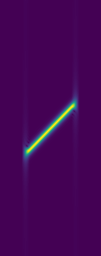
\includegraphics[width=.9\textwidth]{./img/signal/chirp_stft.tikz}
        \caption{}
        \label{fig_chirp_2}
    \end{subfigure}
    \caption{线性调频信号示意图 (a) 信号实部 (b) 短时傅里叶变换结果}
    \label{fig_chirp}
\end{figure}

为了进一步提升系统的抗干扰能力与目标检测性能,可采用非线性调频技术,其瞬时相位函数可以有多种形式,例如:
\begin{enumerate}
    \item 三次相位:$\phi(t) = \frac{\kappa}{2} t^3$,瞬时频率随时间二次变化(如\cref{fig_cubic}所示);
    \item 高次多项式相位:$\phi(t) = \sum_{n=0}^{N} a_n t^n$,可灵活控制频率变化规律;
    \item 正弦相位:$\phi(t) = A \sin(2 \pi f_m t + \phi_0)$,瞬时频率呈周期性波动;
    \item 指数相位:$\phi(t) = A \big(e^{\alpha t} - 1\big)$,瞬时频率按指数规律变化。
\end{enumerate}
这些非线性调频形式能够在特定应用中优化脉冲压缩旁瓣特性,提升目标检测与抗干扰性能。但其实现复杂度相对较高,硬件要求也更为严格。

\begin{figure}[htb!]
    \centering
    \begin{subfigure}{.45\textwidth}
        \centering
        \includegraphics[width=.9\textwidth]{./img/signal/cubic.tikz}
        \caption{}
        \label{fig_cubic_1}
    \end{subfigure}
    \begin{subfigure}{.45\textwidth}
        \centering
        
\includegraphics[width=.9\textwidth]{./img/signal/cubic_stft.tikz}
        \caption{}
        \label{fig_cubic_2}
    \end{subfigure}
    \caption{三次相位调频信号示意图 (a) 信号实部 (b) 短时傅里叶变换结果}
    \label{fig_cubic}
\end{figure}


相位编码是一种通过在发射信号中引入离散相位变化来实现调制的技术,其核心思想是在信号持续时间内按照预定的编码序列对载波相位进行跳变。常见的相位编码方式包括:
\begin{enumerate}
    \item 二相编码(Binary Phase Shift Keying, BPSK):相位取 $\{0, \pi\}$ 两个值,对应发射信号符号为 $\{+1, -1\}$,典型代表为 Barker 码(如\cref{fig_barker}所示);
    \item 多相编码(M-ary Phase Shift Keying, MPSK):相位在 $M$ 个等间隔值之间跳变,例如四相编码(Quadrature Phase Shift Keying,QPSK)取 $\{0, \pi/2, \pi, 3\pi/2\}$;
    \item Frank 编码:将信号分为若干子脉冲,每个子脉冲的相位按二维矩阵规律编码,可实现较低旁瓣;
    \item P1--P4 编码:适用于脉冲压缩的特殊多相编码序列,通过相位设计获得理想的自相关特性。
\end{enumerate}
相位编码实现相对简单,主要通过数字信号处理技术对信号进行离散化和相位调制。其优点在于能够灵活控制信号的频谱特性,提高抗干扰能力,但对硬件实现要求较高。

\begin{figure}[htb!]
    \centering
    \includegraphics[width=.4\textwidth]{./img/signal/barker13.tikz}
    \caption{Barker-13 相位编码示意图}
    \label{fig_barker}
\end{figure}

若系统的接收天线与发射天线共用或距离较近,则在理想情况下,接收信号可表示为
\[
    r(t) = \sum_{k=1}^{K} A_k s\left(t - \frac{2 R_k}{c}\right),
\]
其中,$K$ 为目标数量,$A_k$ 为一个复数,包含了目标反射信号的幅度与相位信息,$R_k$ 表示第 $k$ 个目标与雷达间的距离,$c$ 为光速。通过检测接收信号中是否包含与发射信号相匹配的特征,并估计相应的时延,即可实现对目标的检测与定位。

\section{阵列接收信号模型}

\subsection{一维均匀线性阵列}
单天线雷达只能获取目标的距离信息,若需进一步测量目标方位,通常需要配备具有指向性的天线,并借助机械旋转实现目标定位。然而,此类雷达系统往往依赖体积庞大且易损的伺服机构。为克服这些缺点,相控阵雷达(Phased Array Radar)应运而生。相控阵雷达利用多天线阵列同时接收信号,并通过分析各接收通道间的相位差,实现对目标方位的精确测量。

以一维均匀线性阵列(Uniform Linear Array, ULA)为例,设有 $M$ 个天线单元(阵元),且阵元间距为 $d$。在目标足够远的情况下,目标反射的电磁波可以近似看作是平面波。

\begin{figure}[htb!]
    \centering
    \includegraphics[width=.6\textwidth]{./img/signal/array_model.tikz}
    \caption{一维线性阵列示意图}
    \label{fig_array}
\end{figure}

如 \cref{fig_array} 所示,设第 $k$ 个目标与阵列天线的连线与阵列法向之间的夹角为 $\theta_k$。则第 $0$ 个阵元接收到的回波信号,相较于第 $1$ 个阵元接收到的信号,其传播路径多出 $d \sin\theta_k$ 的距离。依次类推,第 $m$ 个阵元接收到的信号,相较于第 $0$ 个阵元接收到的信号,其传播路径多出 $m d \sin\theta_k$ 的距离。不妨以第0个阵元为参考,令其接收到的第\( k \)个目标的回波信号为
\[
    r_k(t) = A_k s\left(t - \frac{2 R_k}{c}\right),
\]
则第 $m$ 个阵元接收到的信号为
\[
    r_k^{(m)}(t) = A_k s\left(t - \frac{2 R_k - m d \sin\theta_k}{c}\right).
\]

将发射信号的基本模型
\[
    s(t) = \operatorname{rect}\left(\frac{t}{T}\right) p(t) e^{j 2 \pi f_c t},
\]
代入线性阵列接收信号模型,可得
\[
    \small
    r_k^{(m)}(t) = A_k \operatorname{rect}\left(\frac{t - \frac{2 R_k - m d \sin\theta_k}{c}}{T}\right)
    p\left(t - \frac{2 R_k - m d \sin\theta_k}{c}\right)
    e^{j 2 \pi f_c \left(t - \frac{2 R_k - m d \sin\theta_k}{c}\right)},
\]
注意到,对于矩形窗函数和低频包络信号,额外的时延 $\frac{m d \sin\theta_k}{c}$ 对其影响可以忽略不计。于是,上式可近似为
\[
    \begin{split}
        r_k^{(m)}(t) \approx & A_k \operatorname{rect}\left(\frac{t - \frac{2 R_k}{c}}{T}\right)
        p\left(t - \frac{2 R_k}{c}\right)
        e^{j 2 \pi f_c \left(t - \frac{2 R_k - m d \sin\theta_k}{c}\right)}                      \\
        =                    & A_k \operatorname{rect}\left(\frac{t - \frac{2 R_k}{c}}{T}\right)
        p\left(t - \frac{2 R_k}{c}\right)
        e^{j 2 \pi f_c \left(t - \frac{2 R_k}{c}\right)}
        e^{j 2 \pi f_c \frac{m d \sin\theta_k}{c}}                                               \\
        =                    & A_k s\left(t - \frac{2 R_k}{c}\right)
        e^{j 2 \pi f_c \frac{m d \sin\theta_k}{c}}                                               \\
        =                    & r_k(t) e^{j 2 \pi f_c \frac{m d \sin\theta_k}{c}}.
    \end{split}
\]
这表明,不同阵元接收到的回波信号,与第 0 个阵元接收到的信号相比,可近似视为相差一个与\( m \)有关的相位因子。

在实际雷达系统中,连续的接收信号经过模数转换采样,可以得到一系列的离散采样点。设每个阵元的采样点数为 \(L\),则第 \(0\) 个阵元接收到的第 \(k\) 个目标的离散回波信号可表示为列向量
\[
    \bm{r}_k =
    \begin{bmatrix}
        r_k(t_0) & r_k(t_1) & \cdots & r_k(t_{L-1})
    \end{bmatrix}^{\mathrm{T}}.
\]
对于第 \(m\) 个阵元,由于目标方位 \(\theta_k\) 引入了阵元间相位差,其回波信号向量可写为
\[
    \bm{r}^{(m)}_k
    = \bm{r}_k \, e^{j 2 \pi f_c \frac{m d \sin\theta_k}{c}},
\]
其中 \(f_c\) 为载频,\(d\) 为阵元间距,\(c\) 为电磁波传播速度。

将所有 \(M\) 个阵元接收到的第 \(k\) 个目标的回波信号按列排列,可以发现第\( k \)个目标对应的接收信号矩阵是一个秩一矩阵,
\[
    \begin{aligned}
        \mathbf{X}_k
         & = \begin{bmatrix}
                 \bm{r}_k^{(0)} & \bm{r}_k^{(1)} & \cdots & \bm{r}_k^{(M-1)}
             \end{bmatrix}                                                           \\
         & = \begin{bmatrix}
                 \bm{r}_k & \bm{r}_k e^{j 2 \pi f_c \frac{d \sin\theta_k}{c}} & \cdots & \bm{r}_k e^{j 2 \pi f_c \frac{(M-1) d \sin\theta_k}{c}}
             \end{bmatrix} \\
         & = \bm{r}_k
        \begin{bmatrix}
            1 & e^{j 2 \pi f_c \frac{d \sin\theta_k}{c}} & \cdots & e^{j 2 \pi f_c \frac{(M-1) d \sin\theta_k}{c}}
        \end{bmatrix}^{\mathrm{T}}                               \\
         & = \bm{r}_k \bm{a}_k^{\mathrm{T}},
    \end{aligned}
\]
其中
\[
    \bm{a}_k =
    \begin{bmatrix}
        1 & e^{j 2 \pi f_c \frac{d \sin\theta_k}{c}} & \cdots & e^{j 2 \pi f_c \frac{(M-1) d \sin\theta_k}{c}}
    \end{bmatrix}^{\mathrm{T}}
\]
称为\textbf{导向矢量}(Steering Vector),其相位包含了目标的方位信息。如图\ref{fig_array_angle}所示,当目标位于阵列的正前方时,所有阵元接收到的信号相位相同;当目标偏离阵列的正前方时,不同阵元接收到的信号之间会存在相位差。

\begin{figure}[htb!]
    \centering
    \begin{subfigure}{.23\textwidth}
        \centering
        \includegraphics[width=.9\textwidth]{./img/signal/array_angle_0.tikz}
        \caption{}
        \label{fig_array_angle_1}
    \end{subfigure}
    \begin{subfigure}{.23\textwidth}
        \centering
        \includegraphics[width=.9\textwidth]{./img/signal/array_angle_p.tikz}
        \caption{}
        \label{fig_array_angle_2}
    \end{subfigure}
    \begin{subfigure}{.23\textwidth}
        \centering
        \includegraphics[width=.9\textwidth]{./img/signal/array_angle_n.tikz}
        \caption{}
        \label{fig_array_angle_3}
    \end{subfigure}
    \caption{一维线性阵列接收信号示例(仅绘制了实部) (a) 目标角度为0 (b) 目标角度为正 (c) 目标角度为负}
    \label{fig_array_angle}
\end{figure}

因此,在不考虑噪声与干扰的情况下,整个阵列的接收信号矩阵可表示为
\[
    \mathbf{X}
    = \sum_{k=1}^{K} \mathbf{X}_k
    = \sum_{k=1}^{K} \bm{r}_k \, \bm{a}_k^{\mathrm{T}},
\]
这表明理想情况下,对于一维均匀线阵,接收信号矩阵是由多个秩一矩阵叠加而成的。记
\[
    \mathbf{R} = \begin{bmatrix}
        \bm{r}_1 & \bm{r}_2 & \cdots & \bm{r}_K
    \end{bmatrix}, \quad \mathbf{A} = \begin{bmatrix}
        \bm{a}_1 & \bm{a}_2 & \cdots & \bm{a}_K
    \end{bmatrix},
\]
可以验证
\[
    \mathbf{X} = \mathbf{R} \mathbf{A}^{\mathrm{T}}.
\]

\subsection{二维均匀线性阵列}
为了能够在三维空间中对目标进行定位,通常需要使用二维均匀线性阵列。与一维阵列类似,二维阵列的接收信号模型也可以通过导向矢量来表示。

设有一个 \(M \times N\) 的二维均匀线性阵列,阵元间距分别为 \(d_x\) 和 \(d_y\)。方便起见,令该二维阵列位于\( x-y \) 平面上。因此,阵列上的第 \( (m,n) \) 个阵元的坐标可以表示为
\[
    \bm{l}^{(m, n)} = \begin{bmatrix}
        m d_x & n d_y & 0
    \end{bmatrix}^{\mathrm{T}}.
\]
设第\( k \)个目标相对于阵列坐标系的俯仰角为 \(\theta_k\),方位角为 \(\phi_k\)。如\cref{fig_2d_array_eg}所示,根据球面坐标系到直角坐标系的转换关系,指向目标的单位向量可以表示为
\[
    \bm{u}_k = \begin{bmatrix}
        \sin\theta_k \cos\phi_k & \sin\theta_k \sin\phi_k & \cos\theta_k
    \end{bmatrix}^{\mathrm{T}}.
\]

\begin{figure}[htb!]
    \centering
    \includegraphics[width=.4\textwidth]{./img/signal/2d_array_eg.tikz}
    \caption{二维均匀线性阵列示例}
    \label{fig_2d_array_eg}
\end{figure}

类似于一维阵列,二维阵列中的阵元接收到的信号,相较于位于原点处的参考阵元,会引入额外的时延。根据\cref{fig_2d_array_eg},可以发现,第\( (m,n) \)个阵元接收到的信号少走的距离为
\[
    \Delta d^{(m,n)}_k = \bm{u}_k^{\mathrm{T}} \bm{l}^{(m,n)} = m d_x \sin\theta_k \cos\phi_k + n d_y \sin\theta_k \sin\phi_k.
\]
记\( \mu = d_x \sin\theta_k \cos\phi_k \),\( \nu = d_y \sin\theta_k \sin\phi_k \),则第\( (m,n) \)个阵元接收到的信号可以表示为
\[
    \begin{split}
        r^{(m,n)}_k(t) & = A_k s\left(t - \frac{2 R_k - m \mu - n \nu}{c}\right)                                                                                                                                                \\
                       & = A_k \operatorname{rect}\left(\frac{t - \frac{2 R_k - m \mu - n \nu}{c}}{T}\right) p\left(t - \frac{2 R_k - m \mu - n \nu}{c}\right) e^{j 2 \pi f_c \left(t - \frac{2 R_k - m \mu - n \nu}{c}\right)} \\
                       & \approx A_k \operatorname{rect}\left(\frac{t - \frac{2 R_k}{c}}{T}\right) p\left(t - \frac{2 R_k}{c}\right) e^{j 2 \pi f_c \left(t - \frac{2 R_k}{c}\right)} e^{j 2 \pi f_c \frac{m \mu + n \nu}{c}}   \\
                       & = A_k s\left(t - \frac{2 R_k}{c}\right) e^{j 2 \pi f_c \frac{m \mu + n \nu}{c}}                                                                                                                        \\
                       & = r_k(t) e^{j 2 \pi f_c \frac{m \mu + n \nu}{c}}.
    \end{split}
\]
同样地,令\( \bm{r}_k \) 为第\( (0,0) \)个阵元接收到的信号对应的离散向量,则第\( (m,n) \)个阵元接收到的信号向量可以表示为
\[
    \bm{r}_k^{(m,n)} = \bm{r}_k e^{j 2 \pi f_c \frac{m \mu + n \nu}{c}} = \bm{r}_k e^{j 2 \pi f_c \frac{m \mu}{c}} e^{j 2 \pi f_c \frac{n \nu}{c}}.
\]

将所有阵元接收到的第\( k \)个目标反射的信号向量排列成一个\( L \times M \times N \)大小的张量\( \mathcal{X}_k \),则该张量中的元素有如下表达式
\[
    \left( \mathcal{X}_k \right)_{lmn} = \left( \bm{r}_k \right)_l e^{j 2 \pi f_c \frac{m \mu}{c}} e^{j 2 \pi f_c \frac{n \nu}{c}}.
\]
根据\cref{def:outer-product}中的外积定义,不难发现\( \mathcal{X}_k \)是由三个向量的外积构成的:
\[
    \mathcal{X}_k = \bm{r}_k \circ \bm{a}_k \circ \bm{b}_k,
\]
其中\( \bm{a}_k \)和\( \bm{b}_k \)为两个导向矢量,有如下表达式:
\[
    \begin{split}
        \bm{a}_k & = \begin{bmatrix}
                         1 & e^{j 2 \pi f_c \frac{\mu}{c}} & \cdots & e^{j 2 \pi f_c \frac{(M-1) \mu}{c}}
                     \end{bmatrix}^{\mathrm{T}}, \\
        \bm{b}_k & = \begin{bmatrix}
                         1 & e^{j 2 \pi f_c \frac{\nu}{c}} & \cdots & e^{j 2 \pi f_c \frac{(N-1) \nu}{c}}
                     \end{bmatrix}^{\mathrm{T}}.
    \end{split},
\]

因此,在理想情况下,二维均匀线性阵列的接收信号矩阵是由一系列秩一张量构成的:
\[
    \mathcal{X}
    = \sum_{k=1}^{K} \mathcal{X}_k
    = \sum_{k=1}^{K} \bm{r}_k \circ \bm{a}_k \circ \bm{b}_k.
\]
进一步地,根据\cref{prop:diag-kron},张量\( \mathcal{X} \)可以写成如下形式:
\[
    \begin{split}
        \mathcal{X} = \mathcal{I}_K \times_1 \mathbf{R} \times_2 \mathbf{A} \times_3 \mathbf{B}.
    \end{split},
\]
其中\( \mathcal{I}_K \)为一个\( K \times K \times K \)的对角张量,其对角元素都为1,而\( \mathbf{R} \)、\( \mathbf{A} \)和\( \mathbf{B} \)分别为接收信号、导向矢量的矩阵表示:
\[
    \mathbf{R} = \begin{bmatrix}
        \bm{r}_1 & \cdots & \bm{r}_K
    \end{bmatrix}, \quad
    \mathbf{A} = \begin{bmatrix}
        \bm{a}_1 & \cdots & \bm{a}_K
    \end{bmatrix}, \quad
    \mathbf{B} = \begin{bmatrix}
        \bm{b}_1 & \cdots & \bm{b}_K
    \end{bmatrix}.
\]

当二维阵列的第二个维度\( N=1 \)时,此时阵列退化为一维阵列,接收张量可以表示为
\[
    \mathcal{X} = \mathcal{I}_K \times_1 \mathbf{R} \times_2 \mathbf{A}.
\]
根据\cref{prop:apx_kron_matmul},可以发现该接收张量的表示形式与一维阵列的情况等价,即
\[
    \mathcal{X} = \mathcal{I}_K \times_1 \mathbf{R} \times_2 \mathbf{A} = \mathbf{R} \mathbf{A}^{\mathrm{T}}.
\]

\section{多普勒接收信号模型}


\section{空时联合接收信号模型}

\section{噪声、杂波和多径模型}

\chapter{雷达信号检测}
在雷达系统中,目标检测是由接收信号处理走向目标识别的关键环节。其核心任务是从含有噪声、杂波与多径效应的复杂回波中,可靠地区分目标与干扰。为了提升检测性能,雷达信号处理往往需要经过脉冲压缩以提高距离分辨率,通过脉冲积累增强信噪比,最终在统计意义下实现目标检测。

本章将依次介绍:首先讨论脉冲压缩原理及其在提高雷达分辨率中的作用;随后分析非相干积累与相干积累两类脉冲积累方法的特点与适用场景;最后重点研究目标检测的统计理论,包括虚警率、检测率、门限选择与恒虚警率(CFAR)检测等经典方法。

\section{脉冲压缩}
如\cref{sec_radar_signal_model}所述,早期雷达系统往往难以同时兼顾距离分辨率与目标检测性能。为在保持较高距离分辨率的同时提升检测效能,现代雷达通常在低频包络中引入时间调制以拓展信号带宽,从而增强系统的抗干扰能力与目标检测能力。以线性调频信号为例,其回波信号的实部如\cref{fig_chirp_eg}所示。在实际应用中,由于噪声等因素的存在,往往难以直接确定回波脉冲的上升沿;此外,若仅依靠上升沿来估计脉冲时延,也无法有效解决距离分辨率与检测性能之间的固有矛盾。

\begin{figure}[htb!]
    \centering
    \includegraphics[width=.6\textwidth]{./img/detection/chirp_eg.tikz}
    \caption{线性调频回波信号示意图}
    \label{fig_chirp_eg}
\end{figure}

需要注意的是,\cref{fig_chirp_eg} 中仅绘制了回波信号的低频包络部分。这是因为在实际应用中,回波信号通常会先经过下变频处理,再进行采样。经过这一过程,高频载波成分被滤除,仅保留下变频后的低频信息。因此,本章讨论的信号均不再考虑高频载波。

为克服这一难题,雷达信号处理中引入了脉冲压缩(Pulse Compression)技术。该方法通过在发射端发送宽脉冲、在接收端对回波进行匹配滤波,实现了``能量积累''与``时间压缩''的统一。由此,雷达既能在保持高能量积累以提高检测概率的同时,又获得等效的窄脉冲,从而显著提升距离分辨率。

设\( \bm{s} \in \mathbb{C}^{W \times 1} \)为发射信号对应的离散时间序列向量,也称作参考向量,\( \bm{x} \in \mathbb{C}^{L \times 1} \)为接收信号对应的离散时间序列向量。此时,问题就转换成从回波向量\( \bm{x} \)中找到与发射向量相似的序列。不妨将\( \bm{x} \)排列成如下的矩阵形式
\[
    \mathbf{X} = \begin{bmatrix}
        x_1    & x_2     & \cdots & x_{L-W+1} \\
        x_2    & x_3     & \cdots & x_{L-W+2} \\
        \vdots & \vdots  & \ddots & \vdots    \\
        x_W    & x_{W+1} & \cdots & x_L
    \end{bmatrix} \in \mathbb{C}^{W \times (L-W+1)},
\]
其中矩阵\( \mathbf{X} \)的第\( i \)列记为\( \bm{x}_i \in \mathbb{C}^{W \times 1} \)。显然,我们只需要一一对比所有的\( \bm{x}_i \)与\( \bm{s} \)的相似性,如果相似度比较高,那么就可以认为在该位置存在回波信号,自然就能确定对应的时延了。最常见的衡量相似度的指标是余弦相似度(Cosine Similarity),其定义如下
\begin{definition}
    设有两个向量\( \bm{a}, \bm{b} \in \mathbb{C}^{n \times 1} \),则它们的余弦相似度有如下计算公式
    \[
        S(\bm{a}, \bm{b}) = \frac{\bm{a}^{\mathrm{H}} \bm{b}}{\|\bm{a}\| \|\bm{b}\|}
    \]
    其中\( \bm{a}^{\mathrm{H}} \)为\( \bm{a} \)的共轭转置。余弦相似度越大,一定程度上表示两个向量越相似。
\end{definition}

因此,依次计算所有的
\[
    y_i = S(\bm{x}_i, \bm{s}),
\]
即可得到脉冲压缩后的输出结果:
\[
    \bm{y} = \begin{bmatrix} y_1 & y_2 & \cdots & y_{L-W+1} \end{bmatrix}^{\mathrm{T}}
    \in \mathbb{C}^{(L-W+1) \times 1}.
\]
然而,余弦相似度的计算在硬件实现中相对复杂,因此在实际应用中往往需要进一步简化。注意到参考向量 \( \bm{s} \) 是已知的,不妨提前归一化\footnote{后文均默认\( \bm{s} \)为归一化后的向量},令其模长\( \left\| \bm{s} \right\| = 1 \)。于是余弦相似度可简化为
\[
    y_i = \frac{\bm{x}_i^{\mathrm{H}} \bm{s}}{\|\bm{x}_i\|}.
\]
但在工程实现中,计算 \( \|\bm{x}_i\| \) 仍然存在一定开销。

为克服这一问题,可以预先对接收向量 \( \bm{x} \) 进行归一化,使得不同距离单元处的信号能量保持在相近水平。根据雷达方程\cref{eq:radar_equation},接收信号的功率随目标距离的四次方衰减。因此,可以利用这一先验规律,对回波信号施加随时间(或距离)变化的自动增益控制:距离越远,信号衰减越严重,所需增益越大。这样便能在不显著增加硬件复杂度的前提下,近似实现归一化处理。在这种情况下,余弦相似度可近似简化为一个内积形式:
\[
    y_i =  \bm{x}_i^{\mathrm{H}} \bm{s},
\]
并可以进一步写成矩阵乘法的形式:
\[
    \bm{y} = \mathbf{X}^{\mathrm{H}} \bm{s}.
\]

由\cref{apx.conv-corr-mat}可知,该形式实质上对应一次相关运算,即将原始回波信号与参考信号进行相关处理。进一步地,相关运算可以等价地转化为卷积运算,而卷积又可视为一个有限冲激响应(Finite Impulse Response, FIR)滤波器,其滤波器系数正是参考信号的共轭翻转序列。因此,该处理过程通常被称为\emph{匹配滤波}。方便起见,我们直接称\( \bm{s} \)为匹配滤波器的滤波器系数。

\begin{example}\label{eg_pc}
    对\cref{fig_pc_eg1}中的接收信号进行匹配滤波处理。
    \begin{figure}[htb!]
        \centering
        \includegraphics[width=.6\textwidth]{./img/detection/pc_eg1.tikz}
        \caption{接收信号示意图(仅绘制了实部)}
        \label{fig_pc_eg1}
    \end{figure}
\end{example}
\begin{solution}
    从原始回波信号可以看出,噪声干扰较为明显。若仅依靠脉冲的上升沿进行判别,只能大致识别出两个目标回波。而经过匹配滤波处理后,不仅能够清晰地区分出三个目标回波,而且噪声得到了有效抑制,其结果如\cref{fig_pc_eg2}所示。由于匹配滤波能够将宽脉冲在时域中压缩为尖锐的脉冲峰,这一过程通常也被称为脉冲压缩。
    \begin{figure}[htb!]
        \centering
        \includegraphics[width=.6\textwidth]{./img/detection/pc_eg2.tikz}
        \caption{脉冲压缩结果}
        \label{fig_pc_eg2}
    \end{figure}

    令\( A \)为回波对应的幅度与相位信息,并假设噪声的均值\( \mu_n \)为零,方差为\( \sigma_n^2 \),则对于回波处的采样点,其均值为
    \[
        \mu_s = \operatorname{E}[A s_k + n] = A s_k,
    \]
    其中\( s_k \)为参考信号的第\( k \)个采样点, \( n \) 为噪声项。注意到,对于线性调频信号而言,归一化后的参考向量\( \bm{s} \in \mathbb{C}^{W \times 1} \)中的元素\( s_k \)的模值均为\( \frac{1}{\sqrt{W}} \)。因此,根据信噪比的定义\footnote{本书中,信噪比均采用偏转系数(Deflection Coefficient)定义,即\( SNR = \frac{|\mu_s - \mu_n|^2}{\sigma_n^2} \),其中\( \mu_s \) 和 \( \mu_n \) 分别为目标和噪声的均值,\( \sigma_n^2 \) 为噪声的方差。当噪声均值为零时,偏转系数与经典信噪比形式一致。},可以得到原始回波信号的信噪比为
    \[
        \mathrm{SNR}_{a} = \frac{(\mu_s - \mu_n)^2}{\sigma^2} = \frac{|A s_k - 0|^2}{\sigma^2} = \frac{|A|^2}{\sigma^2 W}.
    \]

    不妨令向量\( \bm{x}_i = A \bm{s} + \bm{n}_i \)对应了目标的回波信号,其中\(\bm{n}_i\) 为噪声向量。那么脉压后,目标对应的尖值取值的均值为
    \[
        \mu_s = \operatorname{E}[\bm{x}_i^{\mathrm{H}} \bm{s}] = \operatorname{E}[(A \bm{s} + \bm{n}_i)^{\mathrm{H}} \bm{s}] = A \bm{s}^{\mathrm{H}} \bm{s} + \operatorname{E}[\bm{n}_i^{\mathrm{H}} \bm{s}] = A.
    \]
    与此同时,令\( \bm{x}_j = \bm{n}_j \)为噪声对应的向量,其不包含目标回波,则对应的脉压结果的均值为
    \[
        \mu_n = \operatorname{E}[\bm{n}_j^{\mathrm{H}} \bm{s}] = 0,
    \]
    方差为
    \[
        \sigma^2 = \operatorname{E}[|\bm{n}_j^{\mathrm{H}} \bm{s} - 0|^2] = \operatorname{E}[\bm{s}^{\mathrm{H}} \bm{n}_j \bm{n}_j^{\mathrm{H}} \bm{s}] = \sigma^2 \bm{s}^{\mathrm{H}} \mathbf{I} \bm{s} = \sigma^2.
    \]
    因此,脉冲压缩后的信噪比为
    \[
        \mathrm{SNR}_{b} = \frac{|A-0|^2}{\sigma^2} = \frac{|A|^2}{\sigma^2}.
    \]
    综上,脉冲压缩的信噪比提升倍数为
    \[
        \frac{\mathrm{SNR}_{b}}{\mathrm{SNR}_{a}} = W.
    \]
\end{solution}

既然脉冲压缩本质上是对原始回波信号的一种滤波,而其对应的滤波器系数通常取为参考信号所对应的向量,那么一个自然的问题是:最优的滤波系数是否必然就是参考信号向量?不妨将期望的滤波器系数记为 \( \bm{w} \)。显然,理想的滤波器应在凸显目标回波信号的同时,尽可能抑制非目标分量,例如噪声、干扰和杂波等。基于这一考虑,可以建立如下的优化模型:
\[
    \begin{cases}
        \min\limits_{\bm{w}} \left\| \mathbf{X}^{\mathrm{H}} \bm{w} \right\|^2, \\[6pt]
        \text{s.t. } \bm{s}^{\mathrm{H}} \bm{w} = 1 ,
    \end{cases}
\]
其中,目标函数刻画了滤波器输出的总能量,约束条件保证了参考信号方向上的响应被固定为 1。这样,滤波器在保持对目标信号敏感的同时,能够最大程度地抑制非目标分量的输出。利用\cref{apx.lagrange-multiplier}介绍的拉格朗日乘数法,可以获得该优化问题的解析解。首先,构建拉格朗日函数
\[
    \mathcal{L}(\bm{w}, \lambda) = \frac{1}{2}\left\| \mathbf{X}^{\mathrm{H}} \bm{w} \right\|^2 - \lambda \left( \bm{s}^{\mathrm{H}} \bm{w} - 1 \right).
\]
对\( \bm{w} \)和\( \lambda \)分别求导,并令其为0,得到方程组
\[
    \begin{cases}
        \frac{\partial \mathcal{L}}{\partial \bm{w}} = \mathbf{X} \mathbf{X}^{\mathrm{H}} \bm{w} - \lambda \bm{s} = 0 \\
        \frac{\partial \mathcal{L}}{\partial \lambda} = \bm{s}^{\mathrm{H}} \bm{w} - 1 = 0
    \end{cases}.
\]
联立上述方程组,得到
\[
    \begin{cases}
        \lambda = \frac{1}{\bm{s}^{\mathrm{H}} \mathbf{X} \mathbf{X}^{\mathrm{H}} \bm{s}} \\
        \bm{w} = \frac{\mathbf{X} \mathbf{X}^{\mathrm{H}} \bm{s}}{\bm{s}^{\mathrm{H}} \mathbf{X} \mathbf{X}^{\mathrm{H}} \bm{s}}
    \end{cases}.
\]
从中可以看出,最优的滤波器系数 \( \bm{w} \) 并不等于参考信号 \( \bm{s} \)。但注意到,当我们假设信号中只存在高斯白噪声时,数据的协方差矩阵近似为一个对角矩阵\( \frac{1}{L-W+1} \mathbf{X} \mathbf{X}^{\mathrm{H}} \approx \sigma^2 \mathbf{I} \),其中\( \mathbf{I} \)为单位矩阵。此时,最优的滤波器系数 \( \bm{w} \) 近似为
\[
    \bm{w} \approx \frac{ \mathbf{I} \bm{s}}{\bm{s}^{\mathrm{H}} \mathbf{I} \bm{s}} = \frac{\bm{s}}{\bm{s}^{\mathrm{H}} \bm{s}} = \bm{s}.
\]
这表明,在仅含白噪声的理想环境下,最优的滤波器系数近似等于参考向量。

此外需要注意,脉冲压缩后的输出脉冲实际上对应于参考向量的自相关,因此其波形形状与参考向量(低频包络)密切相关。注意到,发射信号的低频包络由两部分组成
\[
    s(t) = \operatorname{rect}\left( \frac{t}{T} \right) p(t).
\]
其自相关函数为
\[
    R_s(\tau) = \operatorname{E}\left[ s(t)s^*(t-\tau)\right]
    = \lim_{T \rightarrow \infty } \frac{1}{T} \int_{-T/2}^{T/2} \operatorname{rect}\left( \frac{t}{T} \right)
    \operatorname{rect}\left( \frac{t-\tau}{T} \right)
    p(t)p^*(t-\tau)dt.
\]
不妨设 \(p(t)\) 为宽平稳随机过程,则其自相关函数\( R_p(\tau) = \mathrm{E}[p(t)p^*(t-\tau)] \) 仅与时间差 \(\tau\) 有关。由此可得近似
\[
    \begin{split}
        R_s(\tau) & \approx R_p(\tau)
        \lim_{T \rightarrow \infty } \frac{1}{T} \int_{-T/2}^{T/2}
        \operatorname{rect}\left( \frac{t}{T} \right)
        \operatorname{rect}\left( \frac{t-\tau}{T} \right) dt                    \\
                  & = R_p(\tau) \operatorname{Tri}\left( \frac{\tau}{T} \right),
    \end{split}
\]
其中 \(\operatorname{Tri}(\cdot)\) 为三角函数,定义为
\[
    \operatorname{Tri}(x) =
    \begin{cases}
        1-|x|, & |x|\leq 1, \\
        0,     & |x|>1.
    \end{cases}
\]

这表明,脉冲压缩输出的脉冲形状近似为\( p(t) \)自相关函数与三角窗的乘积。而一个信号的自相关函数宽度取决于其带宽:带宽越大,自相关函数越窄,反之亦然。若假设 \(p(t)\) 的带宽为 \(B\),则其自相关函数宽度约为 \(1/B\)。另一方面,若两个目标间的距离差为 \(\Delta R\),则其回波经脉冲压缩后的时间间隔为 \(\frac{2\Delta R}{c}\)。因此,只有当\(\frac{2\Delta R}{c} > \frac{1}{B}\)时,两个脉冲才能有效区分。由此可见,脉冲压缩技术能够将雷达的距离分辨率提升至
\[
    \Delta R = \frac{c}{2B}.
\]

\cref{fig_mf}展示了不同低频包络信号及其脉冲压缩结果,从中可以发现信号带宽越大,脉冲压缩后的波形越尖锐。

\begin{figure}[htb!]
    \centering
    \begin{subfigure}{.3\textwidth}
        \centering
        \includegraphics[width=.9\textwidth]{./img/detection/mf1.tikz}
        \includegraphics[width=.9\textwidth]{./img/detection/mf4.tikz}
        \caption{复指数信号}
        \label{fig_mf_1}
    \end{subfigure}
    \begin{subfigure}{.3\textwidth}
        \centering
        \includegraphics[width=.9\textwidth]{./img/detection/mf2.tikz}
        \includegraphics[width=.9\textwidth]{./img/detection/mf5.tikz}
        \caption{线性调频信号\( \kappa = 20 \)}
        \label{fig_mf_2}
    \end{subfigure}
    \begin{subfigure}{.3\textwidth}
        \centering
        \includegraphics[width=.9\textwidth]{./img/detection/mf3.tikz}
        \includegraphics[width=.9\textwidth]{./img/detection/mf6.tikz}
        \caption{线性调频信号\( \kappa=100 \)}
        \label{fig_mf_3}
    \end{subfigure}
    \caption{不同低频包络信号及其脉冲压缩结果}
    \label{fig_mf}
\end{figure}

在\cref{eg_pc}中,我们已经证明,脉冲压缩所带来的信噪比提升倍数等于参考向量的长度 \(W\)。根据香农采样定理,采样率 \(f_s\) 至少应满足 \(f_s \geq 2B\),其中 \(B\) 为信号带宽。因此,对于时宽为 \(T\) 的发射信号,其参考向量的采样点数至少为
\[
    W = f_s T \geq 2BT.
\]
这表明,脉冲压缩所获得的处理增益与发射信号的时宽和带宽的乘积(Time-Bandwidth Product)成正比。

\section{脉冲积累}
在实际应用中,对于部分微弱目标,即便采用脉冲压缩技术,单次脉冲的信噪比仍可能不足以实现有效检测。此时,可以借助脉冲积累(Pulse Integration)进一步提升信噪比。根据积累过程中是否保留信号的相位信息,脉冲积分类方法可分为两类:其一是对回波进行相位对齐后再叠加的相干积累(Coherent Integration);其二是直接对回波幅度或功率进行统计平均的非相干积累(Non-coherent Integration)。前者能够充分利用信号能量,但对相位同步精度要求较高;后者实现简便,但积累增益有限。

设多普勒雷达系统共发射 \( P \) 个脉冲,并且场景中仅存在一个目标。则脉冲压缩后第 \( p \) 个脉冲对应的尖峰输出为
\[
    y_p = A e^{j \varphi_p} + n_p,
\]
其中 \( A \) 表示目标的幅度与相位信息,\(\varphi_p\) 为第 \( p \) 个脉冲带来的额外相位,\( n_p \) 为服从方差为\( \sigma^2 \)的复高斯分布的随机变量,即\( n_p \sim \mathcal{CN}(0,\sigma^2) \)。此外,噪声处对应的脉冲压缩输出记为 \( w_p \),其与 \( n_p \) 独立同分布。则单脉冲信噪比为
\[
    \mathrm{SNR}_s
    = \frac{\left| \operatorname{E}(y_p) - \operatorname{E}(w_p) \right|^2}{\sigma^2}
    = \frac{|A|^2}{\sigma^2}.
\]

相干积累的基本思想是对各脉冲进行相位补偿后再叠加,得到输出
\[
    y_{\mathrm{ci}} = \sum_{p=1}^P y_p e^{-j \varphi_p} = PA + \sum_{p=1}^P n_p e^{-j \varphi_p}.
\]
相应的噪声输出为
\[
    w_{\mathrm{ci}} = \sum_{p=1}^P w_p e^{-j \varphi_p}.
\]
因此,相干积累后目标的均值为
\[
    \operatorname{E}[y_{\mathrm{ci}}] = PA + \operatorname{E}\left[ \sum_{p=1}^P n_p e^{-j \varphi_p} \right] = PA,
\]
噪声的均值为
\[
    \operatorname{E}[w_{\mathrm{ci}}] = \sum_{p=1}^P \operatorname{E}[w_p] e^{-j \varphi_p} = 0.
\]
由于各个噪声项相互独立,因此其方差为
\[
    \operatorname{Var}[w_{\mathrm{ci}}] =\operatorname{Var}\left[\sum_{p=1}^P w_p e^{-j \varphi_p} \right] = \sum_{p=1}^P \operatorname{Var}[w_p] = P \sigma^2.
\]
由此可得相干积累后的信噪比为
\[
    \mathrm{SNR}_{\mathrm{ci}} = \frac{|PA|^2}{P \sigma^2} = \frac{P|A|^2}{\sigma^2}.
\]

这表明,当有\( P \)个脉冲时,通过相干积累可以将信噪比提升至原来的\( P \)倍。但相干积累要求能够精确地对齐各个脉冲的相位,这在实际应用中可能会难以实现。此时,可以考虑非相干积累的方法,其思想是直接对回波幅度平方进行累加,即
\[
    y_{\mathrm{nci}} = \sum_{p=1}^P |y_p|^2 = \sum_{p=1}^P \left| A e^{j \varphi_p} + n_p \right|^2.
\]
对应的噪声输出为
\[
    w_{\mathrm{nci}} = \sum_{p=1}^P |w_p|^2.
\]
计算可得
\[
    \begin{split}
        \operatorname{E}[y_{\mathrm{nci}}] & = \sum_{p=1}^P \operatorname{E}\left[ |A e^{j \varphi_p} + n_p|^2 \right] = \sum_{p=1}^P \operatorname{E} \left[ |A|^2 + |n_p|^2 + A e^{j \varphi_p} \overline{n}_p + \overline{A} e^{-j \varphi_p} n_p \right] \\
                                           & = \sum_{p=1}^P \left( |A|^2 + \operatorname{E}[|n_p|^2] \right)                                                                                                                                                 \\
                                           & = P |A|^2 + P \sigma^2.
    \end{split}
\]
由于复高斯噪声的模平方服从均值为\( \sigma^2 \)、方差为\( \sigma^4 \)的指数分布。因此,非相干积累后噪声的均值为
\[
    \begin{split}
        \operatorname{E}[w_{\mathrm{nci}}] & = \sum_{p=1}^P \operatorname{E}\left[ |w_p|^2 \right] = P \sigma^2.
    \end{split}
\]
同样,因为\( |w_p|^2 \)之间互相独立,所以噪声的方差为
\[
    \operatorname{Var}[w_{\mathrm{nci}}] = \operatorname{Var}\left[ \sum_{p=1}^P |w_p|^2\right] = \sum_{p=1}^P \operatorname{Var}\left[ |w_p|^2\right] = P \sigma^4.
\]
由此可得非相干积累后的信噪比为
\[
    \mathrm{SNR}_{\mathrm{nci}} = \frac{|P |A|^2 + P \sigma^2 - P \sigma^2|^2}{P \sigma^4} = \frac{P |A|^4}{\sigma^4}.
\]
注意到,非相干积累的输出实质上是各脉冲回波幅度平方的累加,因此在定义信噪比时,通常再取平方根作为最终结果:
\[
    \mathrm{SNR}_{\mathrm{nci}} = \frac{\sqrt{P} |A|^2}{\sigma^2}.
\]

综上所述,相干积累的增益为 \( P \) 倍,而非相干积累的增益仅为 \(\sqrt{P}\) 倍。前者理论增益更大,但实现上对相位同步的依赖更为苛刻;后者实现简单,因而在工程上被广泛采用。

\section{目标检测}
\subsection{虚警率与检测率}
\subsection{门限选择与检测性能}
\subsection{恒虚警率检测}


\chapter{目标参数估计}

在完成信号检测之后,雷达系统还需要进一步提取目标的关键参数,例如方位角、距离、多普勒频率以及极化特征等。这些参数的准确估计不仅关系到目标的定位与跟踪精度,也是后续态势感知与目标识别的重要基础。从算法发展的角度来看,目标参数估计大体经历了几个阶段:最初的经典波束形成方法,随后发展到最小方差处理方法,再到子空间方法和稀疏表示方法。近年来,随着多维观测手段的兴起,多域联合估计方法逐渐受到关注。这类方法能够同时利用空间、多普勒甚至极化等多维信息,从而实现更强的参数解耦和更高的估计精度。

在\cref{sec_radar_signal_model}中,我们介绍了雷达的接收信号模型。对于一个阵列多普勒雷达系统,其接收信号可以表示为一个张量:
\[
    \begin{split}
        \mathcal{X} = \mathcal{I}_K \times_1 \mathbf{R} \times_2 \mathbf{A} \times_3 \mathbf{B} \times_4 \mathbf{P},
    \end{split}
\]
其中,\( K \)为目标数,而矩阵\( \mathbf{R} \)、\( \mathbf{A} \)、\( \mathbf{B} \)和\( \mathbf{P} \)分别包含了目标的距离、方位角、俯仰角、多普勒信息。利用脉冲压缩技术,可以获取目标的距离信息,而本章的重点则是如何进一步从数据中提取目标的方位角和多普勒频率等参数。

\section{波束形成方法}
考虑均匀线性阵列或单阵元在多脉冲下的观测情形,此时,接收信号退化为一个矩阵:
\[
    \mathbf{X} = \mathbf{R} \mathbf{A}^{\mathrm{T}} \in \mathbb{C}^{L \times M},
\]
其中\( \mathbf{R} = \begin{bsmallmatrix} \bm{r}_1 & \bm{r}_2 & \cdots & \bm{r}_K \end{bsmallmatrix} \in \mathbb{C}^{L \times K} \)为目标信号矩阵,\( \mathbf{A} = \begin{bsmallmatrix} \bm{a}_{\omega_1} & \bm{a}_{\omega_2} & \cdots & \bm{a}_{\omega_K} \end{bsmallmatrix} \in \mathbb{C}^{M \times K} \)为阵列流形矩阵(导向矢量矩阵),其列向量为目标的空间或多普勒流形向量,其第\( k \)列通常有如下形式:
\[
    \bm{a}_{\omega_k} = \begin{bmatrix}
        1 & e^{j 2 \pi \omega_k} & \cdots & e^{j 2 \pi (M-1) \omega_k }
    \end{bmatrix}^{\mathrm{T}}.
\]
其中,参数 $\omega_k$ 的物理意义取决于雷达体制:若为阵列雷达,则 $\omega_k = \frac{d}{\lambda}\sin \theta_k$,与目标的方位角 $\theta_k$ 相关;若为单阵元多脉冲雷达,则 $\omega_k = \frac{2 T_r v_k}{\lambda}$,与目标的径向速度 $v_k$ 相关。

波束形成(Beamforming)是最经典的参数估计方法,其基本思想是通过对接收信号进行加权求和,形成一个指向特定方向的空间滤波器或指定速度的多普勒滤波器,从而增强该方向或速度上的信号分量。对于给定滤波器\( \bm{w}_{\omega} \),波束形成的输出可以表示为:
\[
    \bm{y}_{\omega} = \mathbf{X} \bm{w}_{\omega} \in \mathbb{C}^{L \times 1},
\]
可以看作是某个方向或速度上接收到的回波。

\subsection{经典波束形成}

经典波束形成(Conventional Beamforming, CBF)方法利用了不同频率复指数信号在维度充分大时趋于正交的性质,即当 $M$ 足够大时,有
\[
    \frac{1}{M}\bm{a}_{\omega_i}^{\mathrm{H}} \bm{a}_{\omega_j} \approx
    \begin{cases}
        1, & \omega_i = \omega_j,     \\
        0, & \omega_i \neq \omega_j .
    \end{cases}
\]
因此,将滤波器权向量选为与目标流形向量相匹配的形式:
\[
    \bm{w}_{\omega} = \frac{1}{M} \overline{\bm{a}}
    = \frac{1}{M} \begin{bmatrix}
        1 & e^{j 2 \pi \omega} & \cdots & e^{j 2 \pi (M-1) \omega}
    \end{bmatrix}^{\mathrm{H}},
\]
即可有效提取出对应参数值 $\omega$ 的信号分量。该方法又称为 \textbf{Bartlett 波束形成},是最经典的一种波束形成策略。

进一步地,通过扫描不同的参数值\( \omega \),将原始信号投影到不同的方向或速度上,则可以分别获得不同方向或速度上的信号分量。具体而言,对于阵列信号,可以构建如下矩阵:
\[
    \mathbf{W} = \frac{1}{M}\begin{bmatrix}
        1                                                   & 1                                                    & \cdots & 1                                                   \\
        e^{- j 2 \pi \frac{d \sin \theta_1}{\lambda}}       & e^{- j 2 \pi \frac{d \sin \theta_2}{\lambda}}        & \cdots & e^{- j 2 \pi \frac{d \sin \theta_N}{\lambda}}       \\
        \vdots                                              & \vdots                                               & \cdots & \vdots                                              \\
        e^{- j 2 \pi \frac{(M-1) d \sin \theta_1}{\lambda}} & e^{- j 2 \pi \frac{ (M-1) d \sin \theta_2}{\lambda}} & \cdots & e^{- j 2 \pi \frac{(M-1) d \sin \theta_N}{\lambda}}
    \end{bmatrix}\in \mathbb{C}^{M \times N},
\]
其中,\( \theta_1, \theta_2, \cdots, \theta_N \)为扫描的角度值。对于多脉冲信号,可以构建类似的矩阵:
\[
    \mathbf{W} = \frac{1}{M}\begin{bmatrix}
        1                                             & 1                                             & \cdots & 1                                             \\
        e^{- j 2 \pi \frac{2 T_r v_1}{\lambda}}       & e^{- j 2 \pi \frac{2 T_r v_2}{\lambda}}       & \cdots & e^{- j 2 \pi \frac{2 T_r v_N}{\lambda}}       \\
        \vdots                                        & \vdots                                        & \cdots & \vdots                                        \\
        e^{- j 2 \pi \frac{2 (M-1) T_r v_1}{\lambda}} & e^{- j 2 \pi \frac{2 (M-1) T_r v_2}{\lambda}} & \cdots & e^{- j 2 \pi \frac{2 (M-1) T_r v_N}{\lambda}}
    \end{bmatrix} \in \mathbb{C}^{M \times N},
\]
其中,\( v_1, v_2, \cdots, v_N \)为扫描的速度值。对应的波束形成可以表示为如下的矩阵乘法:
\[
    \mathbf{Y} = \mathbf{X} \mathbf{W} \in \mathbb{C}^{L \times N}.
\]
有趣的是,对于多脉冲信号,当所选扫描速度 $v_n$ 满足
\[
    \frac{2 T_r v_n}{\lambda} = \frac{n-1}{M}, \quad n = 1, 2, \cdots, N
\]
时,波束形成矩阵 $\mathbf{W}$ 正好对应于一个 $M \times M$ 的离散傅里叶变换(Discrete Fourier Transform,DFT)矩阵的前 $N$ 行。特别地,当 $M = N$ 时,$\mathbf{W}$ 即为标准的 DFT 矩阵。在这种情况下,波束形成过程等价于对接收信号在参数维度(慢时间维)上进行离散傅里叶变换,从而实现对多普勒频率的估计。

此外,根据\cref{apx.conv-corr-mat}中的结论,对 $\mathbf{X}$ 的列向量 $\bm{x}_i$ 进行脉冲压缩同样可以写成矩阵乘法形式:
\[
    \bm{y}_i = \mathbf{S}^{\mathrm{H}}\bm{x}_i,
\]
其中,$\mathbf{S}$ 为由参考向量构造的矩阵,有如下形式:
\[
    \mathbf{S} =
    \begin{bmatrix}
        s_1    & 0       & \cdots & 0      \\
        s_2    & s_1     & \cdots & 0      \\
        \vdots & \vdots  & \ddots & \vdots \\
        s_W    & s_{W-1} & \ddots & s_1    \\
        0      & s_W     & \ddots & s_2    \\
        \vdots & \vdots  & \ddots & \vdots \\
        0      & 0       & \cdots & s_W
    \end{bmatrix}.
\]
由此可见,当同时对接收信号矩阵 $\mathbf{X}$ 的行向量与列向量分别实施波束形成与脉冲压缩时,其结果可统一表示为
\[
    \mathbf{Z} = \mathbf{S}^{\mathrm{H}} \mathbf{X}\mathbf{W}.
\]

在矩阵 $\mathbf{Z}$ 中,目标表现为显著的峰值,其位置对应目标的距离及其他参数(方位或径向速度)。换言之,波束形成可视为在参数维度上的匹配滤波,即对目标信号执行``参数域脉冲压缩''。结合距离维与参数维的双重脉冲压缩,便可实现目标的定位与参数估计。

\begin{example}
    对\cref{fig_data_x}中的接收数据矩阵\( \mathbf{X} \)进行脉冲压缩和波束形成处理。

    \begin{figure}[htb!]
        \centering
        % \includegraphics[width=.4\textwidth]{./img}
        \begin{tikzpicture}
            \begin{axis}[
                    xlabel={参数维},
                    ylabel={时间维},
                    enlargelimits=false,
                    width=4.5cm, height=4.5cm,
                    ytick=\empty,
                    xtick=\empty,
                    ticklabel style={font=\small},
                    label style={font=\small},
                    axis on top
                ]
                \addplot graphics [
                        xmin=-1, xmax=1, ymin=-1, ymax=1,
                    ] {./img/estimation/est_1.png};
            \end{axis}
        \end{tikzpicture}
        \caption{接收数据矩阵\( \mathbf{X} \)(仅绘制了实部)}
        \label{fig_data_x}
    \end{figure}
\end{example}

\begin{solution}
    处理结果如\cref{fig_compressed}所示。\cref{fig_compressed_1} 给出了对 \( \mathbf{X} \) 的行向量进行脉冲压缩的结果:原本具有一定展宽的目标回波在压缩后转变为尖锐的脉冲,在图像中表现为水平直线;同时,由于两个目标对应的直线具有不同的频率起伏,说明其参数值(方位或速度)存在差异。

    \cref{fig_compressed_2} 展示了对 \( \mathbf{X} \) 的行向量进行波束形成的结果:两个目标在参数维上也被压缩为尖锐的脉冲,在图像中对应两条垂直直线,并且这两条直线明显呈现出 Chirp 信号的特征。

    \cref{fig_compressed_3} 则给出了在行向量和列向量上分别进行脉冲压缩与波束形成的联合结果:此时,两个目标在距离维和参数维均被压缩为尖锐脉冲,在图像中表现为两个亮点,其位置正好对应目标的距离和参数值。

    \begin{figure}[htb!]
        \centering
        \begin{subfigure}{.3\textwidth}
            \centering
            \begin{tikzpicture}
                \begin{axis}[
                        xlabel={参数维},
                        ylabel={时间维},
                        enlargelimits=false,
                        width=4.5cm, height=4.5cm,
                        ytick=\empty,
                        xtick=\empty,
                        ticklabel style={font=\small},
                        label style={font=\small},
                        axis on top
                    ]
                    \addplot graphics [
                            xmin=-1, xmax=1, ymin=-1, ymax=1,
                        ] {./img/estimation/est_2.png};
                \end{axis}
            \end{tikzpicture}
            \caption{\( \mathbf{S}\mathbf{X} \)实部}
            \label{fig_compressed_1}
        \end{subfigure}
        \begin{subfigure}{.3\textwidth}
            \centering
            \begin{tikzpicture}
                \begin{axis}[
                        xlabel={参数维},
                        ylabel={时间维},
                        enlargelimits=false,
                        width=4.5cm, height=4.5cm,
                        ytick=\empty,
                        xtick=\empty,
                        ticklabel style={font=\small},
                        label style={font=\small},
                        axis on top
                    ]
                    \addplot graphics [
                            xmin=-1, xmax=1, ymin=-1, ymax=1,
                        ] {./img/estimation/est_3.png};
                \end{axis}
            \end{tikzpicture}
            \caption{\( \mathbf{X}\mathbf{W} \)实部}
            \label{fig_compressed_2}
        \end{subfigure}
        \begin{subfigure}{.3\textwidth}
            \centering
            \begin{tikzpicture}
                \begin{axis}[
                        xlabel={参数维},
                        ylabel={时间维},
                        enlargelimits=false,
                        width=4.5cm, height=4.5cm,
                        ytick=\empty,
                        xtick=\empty,
                        ticklabel style={font=\small},
                        label style={font=\small},
                        axis on top
                    ]
                    \addplot graphics [
                            xmin=-1, xmax=1, ymin=-1, ymax=1,
                        ] {./img/estimation/est_4.png};
                \end{axis}
            \end{tikzpicture}
            \caption{\(  \mathbf{S}\mathbf{X}\mathbf{W} \)幅度}
            \label{fig_compressed_3}
        \end{subfigure}
        \caption{距离维和参数维二重脉冲压缩示意图}
        \label{fig_compressed}
    \end{figure}
\end{solution}

在某些情况下,我们可能并不关心目标的距离信息,而仅希望获得其参数信息(如方位或速度)。此时,可以直接利用波束形成后的输出计算参数维度上的功率谱。具体地,对于参数值 $\omega$,对应输出的功率可表示为
\[
    p_{\omega} = \frac{1}{L}\|\bm{y}_{\omega}\|_2^2
    = \frac{1}{L}\|\mathbf{X}\bm{w}_{\omega}\|_2^2
    = \frac{1}{L}\bm{w}_{\omega}^{\mathrm{H}}\mathbf{X}^{\mathrm{H}}\mathbf{X}\bm{w}_{\omega}
    = \bm{w}_{\omega}^{\mathrm{H}} \mathbf{\Sigma}_{\mathbf{X}} \bm{w}_{\omega},
\]
其中,$\mathbf{\Sigma}_{\mathbf{X}} = \frac{1}{L}\mathbf{X}^{\mathrm{H}}\mathbf{X}$ 为接收信号矩阵的协方差矩阵(一般假设接收信号均值为零)。通过对不同参数值 $\omega$ 进行扫描,即可得到参数维度的功率谱估计,从而实现目标参数的直接估计。

对\cref{fig_data_x}中的数据进行波束形成处理,并计算参数维度的功率谱,结果如\cref{fig_spectrum_cbf}所示。可以看到,功率谱在目标参数值处出现了明显的峰值,并且峰值在参数维度上的位置与\cref{fig_compressed_3}中的目标水平位置一致。通过对功率谱进行峰值检测,即可实现目标参数的估计。

\begin{figure}[htb!]
    \centering
    \begin{tikzpicture}
        \begin{axis}[
                xlabel=参数维, ylabel=归一化功率谱,
                ticklabel style={font=\small},
                label style={font=\small},
                % xtick=\empty,ytick=\empty,
                xmin = -0.5, xmax=0.5, ymin=0, ymax=1.2,
                grid, width=8cm, height=4cm,
                legend cell align=left,
                legend style={
                        anchor=north east,
                        font=\tiny,
                        draw=none,
                        fill=none
                    }
            ]
            \addplot[
                c1,
                thick,
            ] table[x=w, y=p, col sep=comma] {./img/estimation/cbf.csv};
        \end{axis}
    \end{tikzpicture}
    \caption{波束形成功率谱估计}
    \label{fig_spectrum_cbf}
\end{figure}

对于阵列信号而言,波束形成的一大优势是可以直接通过移相器硬件实现。通过控制各阵元的相位,对原始模拟信号加权求和,即可在空间上实现对特定方向的滤波。这样只需一路模数转换器对波束形成后的信号进行采样与处理,便能显著节省硬件资源。参数扫描则通过调节移相器的相位来完成,对应的雷达系统称为无源相控阵雷达(Passive Phased Array Radar)。这种方式的缺点在于无法同时观测多个方向的信号分量,因此在目标数量较多或干扰复杂的环境下,性能容易受限。相比之下,若对各阵元的信号分别采样并数字化,再通过数字处理实现波束合成,则能够同时获得多个方向的信号分量,从而提升系统的灵活性与抗干扰能力,但也会增加硬件开销。这类系统即为有源相控阵雷达(Active Phased Array Radar)。

尽管波束形成方法简单直观,但其分辨率和抗干扰能力有限,尤其在目标间距较近或存在强干扰时,性能会显著下降。对于一个特定的参数值\( \omega \),波束形成的输出可以进一步表示为:
\[
    \bm{y}_{\omega} = \mathbf{X} \bm{w}_{\omega} = \sum_{k=1}^{K} \bm{r}_k \bm{a}_{\omega_k}^{\mathrm{T}} \bm{w}_{\omega} = \sum_{k=1}^{K} \bm{r}_k \frac{\bm{a}_{\omega_k}^{\mathrm{T}} \overline{\bm{a}}_{\omega}}{M}.
\]
从中可以发现,波束形成的输出实际上是各个目标回波信号的加权和,对应的权重为\( \frac{\bm{a}_{\omega_k}^{\mathrm{T}} \overline{\bm{a}}_{\omega}}{M} \)。理想情况下,当目标参数值与滤波器参数值相匹配时,该权重接近1,否则趋于0。但在实际应用中,\( M \)的数值有限,此时即便\( \omega_k \neq \omega \)时,对应的权重也可能较大,导致提取出来的信号中混入了其他目标的成分,从而影响估计精度。

注意到
\[
    \begin{split}
        \frac{\bm{a}_{\omega_k}^{\mathrm{T}} \overline{\bm{a}}_{\omega}}{M} & = \frac{1}{M} \sum_{m=0}^{M-1} e^{j 2 \pi m (\omega_k - \omega)} = \frac{1}{M} \frac{1 - e^{j 2 \pi M (\omega_k - \omega)}}{1 - e^{j 2 \pi (\omega_k - \omega)}} \\
                                                                            & = \frac{1}{M} \frac{\sin(\pi M (\omega_k - \omega))}{\sin(\pi (\omega_k - \omega))} e^{j \pi (M-1)(\omega_k - \omega)}.
    \end{split}
\]
可以发现该权重的取值仅和\( M \)以及参数差值\( \omega_k - \omega \)有关。如\cref{fig_weight}所示,随着\( M \)的增大,权重函数的主瓣变窄,旁瓣降低,从而提升了参数分辨能力。

\begin{figure}[htb!]
    \centering
    \begin{tikzpicture}
        \begin{axis}[
                xlabel=$ \omega_k - \omega $, ylabel=权重幅度,
                ticklabel style={font=\small},
                label style={font=\small},
                grid, smooth,
                xmin = -0.5, xmax=0.5, ymin=0, ymax=1,
                width=10cm, height=5cm,
                legend cell align=left,
                clip=false,
                legend style={
                        anchor=north east,
                        font=\tiny,
                        draw=none,
                        fill=none
                    }
            ]
            \addplot[
                c1,
                thick,
            ] table[x=w, y=a1, col sep=comma] {./img/estimation/weight.csv};
            \addlegendentry{\( M=11 \)};
            \addplot[
                c2,
                thick,
            ] table[x=w, y=a2, col sep=comma] {./img/estimation/weight.csv};
            \addlegendentry{\( M=21 \)};
            \addplot[
                c3,
                thick,
            ] table[x=w, y=a3, col sep=comma] {./img/estimation/weight.csv};
            \addlegendentry{\( M=51 \)};
        \end{axis}
    \end{tikzpicture}
    \caption{不同\( M \)值下波束形成权重函数}
    \label{fig_weight}
\end{figure}

\subsection{和差比幅测角}
无源相控阵节约了硬件开销,但其无法同时观测多个方向的信号分量,有源相控阵虽然提升了灵活性,但硬件成本大大增加。为此,雷达系统中常采用一种折衷的方案,即和差比幅测角(Sum–Difference Amplitude Comparison)方法。 该方法通过将阵列划分为多个子阵,并对各子阵的输出进行加权组合,从而在一定程度上兼顾了硬件复杂度与参数估计性能。

不妨考虑一个均匀线性阵列,其阵元总数为 $2M$,并将其划分为两个子阵,每个子阵包含 $M$ 个阵元。对于给定方位角 $\theta$,和差比幅测角方法构造如下两组滤波器:
\[
    \bm{w}_{\text{sum}} = \frac{1}{2M}
    \begin{bmatrix}
        \bm{w}_1 \\
        \bm{w}_2
    \end{bmatrix}, \quad  \bm{w}_{\text{diff}} = \frac{1}{2M}
    \begin{bmatrix}
        \bm{w}_1 \\
        -\bm{w}_2
    \end{bmatrix},
\]
其中,\( \bm{w}_1 \) 和 \( \bm{w}_2 \) 分别为前\( M \) 个阵元和后\( M \) 个阵元的权向量,有如下形式:
\[
    \bm{w}_1 = \begin{bmatrix}
        1                                           \\
        e^{- j 2 \pi \frac{d \sin \theta}{\lambda}} \\
        \vdots                                      \\
        e^{- j 2 \pi \frac{(M-1) d \sin \theta}{\lambda}}
    \end{bmatrix}, \quad
    \bm{w}_2 = \begin{bmatrix}
        e^{- j 2 \pi \frac{M d \sin \theta}{\lambda}}     \\
        e^{- j 2 \pi \frac{(M+1) d \sin \theta}{\lambda}} \\
        \vdots                                            \\
        e^{- j 2 \pi \frac{(2M-1) d \sin \theta}{\lambda}}
    \end{bmatrix}.
\]
记 $\bm{w}_{\text{sum}}$ 为两个子阵的和波束,$\bm{w}_{\text{diff}}$ 为两个子阵的差波束。对于位于方位角 $\theta_k$ 的目标,其波束形成输出分别为
\[
    \bm{y}_{\text{sum}} =  \bm{r}_k \bm{a}_{\omega_k}^{\mathrm{T}} \bm{w}_{\text{sum}},
    \quad
    \bm{y}_{\text{diff}} = \bm{r}_k \bm{a}_{\omega_k}^{\mathrm{T}} \bm{w}_{\text{diff}}.
\]
可以看出,两者在时域波形上保持完全一致,仅在复数比例因子上有所不同,分别为$\bm{a}_{\omega_k}^{\mathrm{T}} \bm{w}_{\text{sum}}$ 和 $\bm{a}_{\omega_k}^{\mathrm{T}} \bm{w}_{\text{diff}}$。该比例因子同时包含幅度与相位信息,其比值正是和差比幅测角所利用的参数。

为了分析这两个幅度的关系,同样将\( \bm{a}_{\omega_k} \) 拆分为两部分:
\[
    \bm{a}_{\omega_k} =
    \begin{bmatrix}
        \bm{a}_{\omega_k,1} \\
        \bm{a}_{\omega_k,2}
    \end{bmatrix},
\]
其中,
\[
    \bm{a}_{\omega_k,1} = \begin{bmatrix}
        1                                           \\
        e^{j 2 \pi \frac{d \sin \theta_k}{\lambda}} \\
        \vdots                                      \\
        e^{j 2 \pi \frac{(M-1) d \sin \theta_k}{\lambda}}
    \end{bmatrix}, \quad
    \bm{a}_{\omega_k,2} = \begin{bmatrix}
        e^{j 2 \pi \frac{M d \sin \theta_k}{\lambda}}     \\
        e^{j 2 \pi \frac{(M+1) d \sin \theta_k}{\lambda}} \\
        \vdots                                            \\
        e^{j 2 \pi \frac{(2M-1) d \sin \theta_k}{\lambda}}
    \end{bmatrix}.
\]
那么,对于和波束,我们有
\[
    \begin{split}
        \bm{a}_{\omega_k}^{\mathrm{T}} \bm{w}_{\text{sum}} & = \frac{1}{2M}\begin{bmatrix}
                                                                               \bm{a}_{\omega_k,1}^{\mathrm{T}} & \bm{a}_{\omega_k,2}^{\mathrm{T}}
                                                                           \end{bmatrix}
        \begin{bmatrix}
            \bm{w}_1 \\
            \bm{w}_2
        \end{bmatrix}                                                                                                                                                                                                                                                                                  \\
                                                           & = \frac{1}{2M} \bm{a}_{\omega_k,1}^{\mathrm{T}} \bm{w}_1 + \frac{1}{2M} \bm{a}_{\omega_k,2}^{\mathrm{T}} \bm{w}_2                                                                                                                          \\
                                                           & = \frac{1}{2M} \bm{a}_{\omega_k,1}^{\mathrm{T}} \bm{w}_1 + \frac{1}{2M} \left( e^{j 2 \pi \frac{M d \sin \theta_k}{\lambda}} \bm{a}_{\omega_k,1}^{\mathrm{T}} \right) \left( e^{-j 2 \pi \frac{M d \sin \theta}{\lambda}} \bm{w}_1 \right) \\
                                                           & = \frac{1 + e^{j 2\pi \frac{M d (\sin \theta_k - \sin \theta)}{\lambda}}}{2M} \bm{a}_{\omega_k,1}^{\mathrm{T}} \bm{w}_1.
    \end{split}
\]
类似地,对于差波束,有
\[
    \begin{split}
        \bm{a}_{\omega_k}^{\mathrm{T}} \bm{w}_{\text{diff}} & = \frac{1}{2M}\begin{bmatrix}
                                                                                \bm{a}_{\omega_k,1}^{\mathrm{T}} & \bm{a}_{\omega_k,2}^{\mathrm{T}}
                                                                            \end{bmatrix}
        \begin{bmatrix}
            \bm{w}_1 \\
            -\bm{w}_2
        \end{bmatrix}                                                                                                                                                                                                                                                                                     \\
                                                            & = \frac{1}{2M} \bm{a}_{\omega_k,1}^{\mathrm{T}} \bm{w}_1 - \frac{1}{2M} \bm{a}_{\omega_k,2}^{\mathrm{T}} \bm{w}_2                                                                                                                            \\
                                                            & = \frac{1}{2M} \bm{a}_{\omega_k,1}^{\mathrm{T}} \bm{w}_1 - \frac{1}{2M} \left( e^{j 2 \pi \frac{M d \sin \theta_k}{\lambda}} \bm{a}_{\omega_k,1}^{\mathrm{T}} \right) \left( e^{-j 2 \pi \frac{M d \sin \theta_k}{\lambda}} \bm{w}_1 \right) \\
                                                            & = = \frac{1 - e^{j 2\pi \frac{M d (\sin \theta_k - \sin \theta)}{\lambda}}}{2M} \bm{a}_{\omega_k,1}^{\mathrm{T}} \bm{w}_1.
    \end{split}
\]

不妨令\( y_{\text{sum}} \)和\( y_{\text{diff}} \)分别为对\( \bm{y}_{\text{sum}} \)和\( \bm{y}_{\text{diff}} \)进行脉冲压缩后的峰值,则有
\[
    \frac{y_{\text{diff}}}{y_{\text{sum}}} = \frac{1 - e^{j 2\pi \frac{M d (\sin \theta_k - \sin \theta)}{\lambda}}}{1 + e^{j 2\pi \frac{M d (\sin \theta_k - \sin \theta)}{\lambda}}}.
\]
记\( \phi = \pi \frac{M d (\sin \theta_k - \sin \theta)}{\lambda} \),则上式可化简为
\[
    \frac{y_{\text{diff}}}{y_{\text{sum}}} = \frac{1 - e^{j 2 \phi}}{1 + e^{j 2 \phi}} = \frac{e^{-j \phi} - e^{j \phi}}{e^{-j \phi} + e^{j \phi}} = \frac{-2j \sin \phi}{2 \cos \phi} =-j \tan \phi.
\]
因此,两个峰值的虚部之比为
\[
    r = \operatorname{Imag}\left( \frac{y_{\text{diff}}}{y_{\text{sum}}} \right) = - \tan \phi = - \tan \left( \pi \frac{M d (\sin \theta_k - \sin \theta)}{\lambda} \right).
\]

注意到,在\( \theta_k \)与\( \theta \)接近的情况下,有
\[
    \sin \theta_k - \sin \theta = 2 \cos \left( \frac{\theta_k + \theta}{2} \right) \sin \left( \frac{\theta_k - \theta}{2} \right) \approx 2 \cos \theta  \frac{\theta_k - \theta}{2} = \cos \theta (\theta_k - \theta).
\]
将其代入上式,得到
\[
    r \approx - \tan \left( \pi \frac{M d \cos \theta}{\lambda} (\theta_k - \theta) \right),
\]
进一步推导,有
\[
    \theta_k \approx \theta + \frac{\lambda}{\pi M d \cos \theta} \arctan (-r).
\]

\cref{fig_ac}展示了\( \theta \)等于0时,目标角度\( \theta_k \)和和差比幅值\( r \)之间的关系曲线。可以看到,随着目标角度偏离扫描角度,和差比幅值呈现出非线性变化的趋势。通过测量和差比幅值\( r \),并结合上述关系式,即可实现对目标方位角\( \theta_k \)的估计。

\begin{figure}[htb!]
    \centering
    \begin{tikzpicture}
        \begin{axis}[
                xlabel=\( \theta_k(\text{度}) \), ylabel=\( r \),
                ticklabel style={font=\small},
                label style={font=\small},
                grid, xmin=-6, xmax=6,
                width=6cm, height=6cm,
                legend cell align=left,
                legend style={
                        anchor=north east,
                        font=\tiny,
                        draw=none,
                        fill=none
                    }
            ]
            \addplot[
                c1,
                thick,
            ] table[x=x, y=y, col sep=comma] {./img/estimation/ac.csv};
        \end{axis}
    \end{tikzpicture}
    \caption{目标角度与和差比幅值关系曲线}
    \label{fig_ac}
\end{figure}

相较于无源相控阵雷达,和差比幅法需要额外增加一路模数转换器。但这一硬件代价带来的好处是,在主瓣范围内,目标角度能够得到更为精确的测量。此外,和差比幅法的计算复杂度也较低,主要涉及简单的加减运算和脉冲压缩处理,适合实时应用。

\subsection{最小方差无失真响应}
经典波束形成方法并未考虑噪声与干扰的统计特性,因此在复杂环境下性能往往受到限制。为此,最小方差无失真响应(Minimum Variance Distortionless Response, MVDR)方法在设计滤波器时引入了噪声与干扰的协方差矩阵,通过优化权向量以最小化输出功率,同时保证对目标信号无失真响应。该方法的发明者为 Jack Capon,因此有时也称为 Capon 算法。

设 \( \bm{w}_{\omega} \) 为待设计的滤波器权向量,则对应的输出为
\[
    \bm{y}_{\omega} = \mathbf{X} \bm{w}_{\omega}.
\]
直观地,我们希望输出 \(\bm{y}_{\omega}\) 尽可能只包含参数值为 \(\omega\) 的目标信号,同时抑制其他信号与噪声干扰。注意到目标信号对应的导向向量为 \(\bm{a}_{\omega}\),因此目标分量在输出中的占比与 \(|\bm{a}_{\omega}^{\mathrm{T}} \bm{w}_{\omega}|\) 成正比。由此可构造如下优化问题:
\[
    \max_{\bm{w}_{\omega}} \frac{|\bm{a}_{\omega}^{\mathrm{T}} \bm{w}_{\omega}|^2}{ \frac{1}{L} \|\bm{y}_{\omega}\|_2^2},
\]
即在保证输出功率尽可能小的前提下,使目标信号成分最大化。该问题可转化为如下形式的约束优化问题:
\[
    \begin{cases}
        \min_{\bm{w}_{\omega}} \quad & \frac{1}{L} \|\bm{y}_{\omega}\|_2^2               \\
        \text{s.t.} \quad            & \bm{a}_{\omega}^{\mathrm{T}} \bm{w}_{\omega} = 1,
    \end{cases}
\]
其中约束条件保证了对目标信号的无失真响应。

记接收信号的协方差矩阵为
\[
    \mathbf{\Sigma}_{\mathbf{X}} = \frac{1}{L} \mathbf{X}^{\mathrm{H}} \mathbf{X},
\]
则目标函数可重写为
\[
    \frac{1}{L} \|\bm{y}_{\omega}\|_2^2
    = \frac{1}{L} \bm{w}_{\omega}^{\mathrm{H}} \mathbf{X}^{\mathrm{H}} \mathbf{X} \bm{w}_{\omega}
    = \bm{w}_{\omega}^{\mathrm{H}} \mathbf{\Sigma}_{\mathbf{X}} \bm{w}_{\omega}.
\]
利用拉格朗日乘子法可得该优化问题的闭式解为
\[
    \bm{w}_{\omega}
    = \frac{\mathbf{\Sigma}_{\mathbf{X}}^{-1} \overline{\bm{a}}_{\omega}}
    {\overline{\bm{a}}_{\omega}^{\mathrm{H}} \mathbf{\Sigma}_{\mathbf{X}}^{-1} \overline{\bm{a}}_{\omega}}.
\]

遍历所有参数值 \(\omega\),即可构造滤波器组矩阵
\[
    \mathbf{W} = \begin{bmatrix} \bm{w}_{\omega_1} & \bm{w}_{\omega_2} & \cdots \end{bmatrix},
\]
并由此得到波束形成的输出矩阵
\[
    \mathbf{Y} = \mathbf{X} \mathbf{W}.
\]
与经典波束形成类似,可通过计算各列向量的功率来获得参数维度的功率谱:
\[
    p_{\omega}
    = \frac{1}{L} \|\bm{y}_{\omega}\|_2^2
    = \bm{w}_{\omega}^{\mathrm{H}} \mathbf{\Sigma}_{\mathbf{X}} \bm{w}_{\omega}
    = \frac{1}{\overline{\bm{a}}_{\omega}^{\mathrm{H}} \mathbf{\Sigma}_{\mathbf{X}}^{-1} \overline{\bm{a}}_{\omega}}.
\]

\begin{example}
    对\cref{fig_noise_capon}中的包含噪声的数据分别进行 CBF 和 Capon 方法处理,计算对应的二维脉压结果和参数维度的功率谱估计。
    \begin{figure}[htb!]
        \centering
        \begin{tikzpicture}
            \begin{axis}[
                    xlabel={参数维},
                    ylabel={时间维},
                    enlargelimits=false,
                    width=5cm, height=5cm,
                    ytick=\empty,
                    xtick=\empty,
                    ticklabel style={font=\small},
                    label style={font=\small},
                    axis on top
                ]
                \addplot graphics [
                        xmin=-1, xmax=1, ymin=-1, ymax=1,
                    ] {./img/estimation/capon_1.png};
            \end{axis}
        \end{tikzpicture}
        \caption{有噪声数据矩阵\( \mathbf{X} \)(仅绘制了实部)}
        \label{fig_noise_capon}
    \end{figure}
\end{example}
\begin{solution}
    二维脉压结果如\cref{fig_compressed}所示。与经典波束形成相比,Capon 方法在参数维度上展现出更高的分辨率,两个目标在参数维上被压缩为更尖锐的脉冲,并且旁瓣水平显著降低,从而提升了目标的可分辨性和检测性能。
    \begin{figure}[htb!]
        \centering
        \begin{subfigure}{.4\textwidth}
            \centering
            \begin{tikzpicture}
                \begin{axis}[
                        xlabel={参数维},
                        ylabel={时间维},
                        enlargelimits=false,
                        width=5cm, height=5cm,
                        ytick=\empty,
                        xtick=\empty,
                        ticklabel style={font=\small},
                        label style={font=\small},
                        axis on top
                    ]
                    \addplot graphics [
                            xmin=-1, xmax=1, ymin=-1, ymax=1,
                        ] {./img/estimation/capon_2.png};
                \end{axis}
            \end{tikzpicture}
            \caption{CBF}
            \label{fig_compressed_capon_1}
        \end{subfigure}
        \begin{subfigure}{.4\textwidth}
            \centering
            \begin{tikzpicture}
                \begin{axis}[
                        xlabel={参数维},
                        ylabel={时间维},
                        enlargelimits=false,
                        width=5cm, height=5cm,
                        ytick=\empty,
                        xtick=\empty,
                        ticklabel style={font=\small},
                        label style={font=\small},
                        axis on top
                    ]
                    \addplot graphics [
                            xmin=-1, xmax=1, ymin=-1, ymax=1,
                        ] {./img/estimation/capon_3.png};
                \end{axis}
            \end{tikzpicture}
            \caption{Capon}
            \label{fig_compressed_capon_2}
        \end{subfigure}
        \caption{CBF 和 Capon 方法处理后的数据矩阵的幅度图}
        \label{fig_compressed_capon}
    \end{figure}

    参数维度的功率谱估计如\cref{fig_compressed_capon2}所示。可以看到,Capon 方法在参数维度上展现出更高的分辨率,两个目标在参数维上被压缩为更尖锐的脉冲,并且旁瓣水平显著降低,有效提升了目标的可分辨性和检测性能。
    \begin{figure}[htb!]
        \centering
        \begin{tikzpicture}
            \begin{axis}[
                    xlabel={参数维}, ylabel={归一化功率谱},
                    ticklabel style={font=\small},
                    xmin=-0.5, xmax=0.5, ymin=0, ymax=1.2,
                    % xtick=\empty,ytick=\empty,
                    width=8cm, height=4cm,
                    label style={font=\small},
                    grid,
                    legend cell align=left,
                    legend style={
                            anchor=north east,
                            font=\tiny,
                            draw=none,
                            fill=none
                        }
                ]
                \addplot[
                    c1,
                    thick,
                ] table[x=w, y=p1, col sep=comma] {./img/estimation/capon.csv};
                \addlegendentry{CBF}
                \addplot[
                    c2,
                    thick,
                ] table[x=w, y=p2, col sep=comma] {./img/estimation/capon.csv};
                \addlegendentry{Capon}
            \end{axis}
        \end{tikzpicture}
        \caption{CBF 和 Capon 方法处理后的数据矩阵的幅度图}
        \label{fig_compressed_capon2}
    \end{figure}
\end{solution}


在实际应用中,由于接收信号的样本数量有限,协方差矩阵的估计往往不够准确,甚至可能不可逆。为缓解这一问题,可以借鉴岭回归(Ridge Regression)的思想,在目标函数中加入权重向量的范数惩罚项,从而得到如下优化模型:
\[
    \begin{aligned}
        \min_{\bm{w}_{\omega}} \quad &
        \bm{w}_{\omega}^{\mathrm{H}} \mathbf{\Sigma}_{\mathbf{X}} \bm{w}_{\omega}
        + \delta \|\bm{w}_{\omega}\|_2^2                                                 \\
        \text{s.t.} \quad            & \bm{a}_{\omega}^{\mathrm{T}} \bm{w}_{\omega} = 1,
    \end{aligned}
\]
其中 \(\delta > 0\) 为正则化参数。利用拉格朗日乘子法,可得其闭式解为
\[
    \bm{w}_{\omega}
    = \frac{(\mathbf{\Sigma}_{\mathbf{X}} + \delta \mathbf{I})^{-1} \,\overline{\bm{a}}_{\omega}}
    {\overline{\bm{a}}_{\omega}^{\mathrm{H}} (\mathbf{\Sigma}_{\mathbf{X}} + \delta \mathbf{I})^{-1} \,\overline{\bm{a}}_{\omega}}.
\]

由此可见,该方法等价于将原协方差矩阵替换为 \(\mathbf{\Sigma}_{\mathbf{X}} + \delta \mathbf{I}\),在保证无失真约束的同时显著改善了矩阵的条件数,从而增强了算法的鲁棒性。这一技巧通常被称为对角加载(Diagonal Loading)。

\section{子空间方法}
从滤波的角度来看,经典波束形成与 Capon 算法本质上都是通过设计权向量,对接收信号矩阵进行加权叠加,以实现对特定参数下的目标回波的增强,以及对噪声和干扰的抑制。不同之处在于,Capon 算法利用接收信号的协方差矩阵,在保证无失真响应的同时最小化输出功率,因此在噪声和干扰抑制方面较经典波束形成更为有效。然而,Capon 算法依然受限于“滤波”这一框架:对于白噪声而言,无论滤波器如何设计,其输出噪声功率的下限始终等于噪声本身。因此,即便在高信噪比条件下,Capon 谱的分辨率仍受限于通道数\( M \),难以满足高精度参数估计的需求。

为突破 Capon 算法的分辨率瓶颈,研究者提出了基于子空间的高分辨率方法。其核心思想不再依赖滤波器权向量的设计,而是通过对接收信号协方差矩阵进行特征分解,将信号与噪声划分到互相正交的子空间中,并利用这种正交性实现参数估计。借助这一几何结构,子空间方法能够获得远超传统滤波框架的分辨能力。典型代表包括 MUSIC 和 ESPRIT 方法,它们利用信号子空间与噪声子空间的正交特性,实现了高分辨率的参数估计。

\subsection{MUSIC方法}
考虑含噪接收信号模型
\[
    \mathbf{X} = \mathbf{R}\mathbf{A}^{\mathrm{T}} + \mathbf{N} \in \mathbb{C}^{L \times M},
\]
其中 \(\mathbf{N}\) 为加性噪声。若噪声为零均值、方差为 \(\sigma^2\) 的白噪声,则其协方差矩阵近似为对角矩阵:
\[
    \mathbf{\Sigma}_{\mathbf{N}}
    = \frac{1}{L}\mathbf{N}^{\mathrm{H}}\mathbf{N}
    \approx \sigma^2 \mathbf{I} \in \mathbb{C}^{M \times M}.
\]

对于信号部分,一般假设各目标对应的距离互不相同,即 \(\mathbf{R}\) 的列向量互相正交。此时信号协方差矩阵可写为
\[
    \mathbf{\Sigma}_{\mathbf{S}}
    = \frac{1}{L}\,\overline{\mathbf{A}}\,\mathbf{R}^{\mathrm{H}}\mathbf{R}\,\mathbf{A}^{\mathrm{T}}
    = \overline{\mathbf{A}}
    \left(\frac{1}{L}\mathbf{R}^{\mathrm{H}}\mathbf{R}\right)
    \mathbf{A}^{\mathrm{T}}
    \approx \overline{\mathbf{A}}\,\mathbf{\Sigma}_{\mathbf{R}}\,\mathbf{A}^{\mathrm{T}},
\]
其中
\[
    \mathbf{\Sigma}_{\mathbf{R}}
    = \frac{1}{L}\mathbf{R}^{\mathrm{H}}\mathbf{R}
    = \operatorname{diag}(\sigma_1^2,\sigma_2^2,\cdots,\sigma_K^2),
\]
其对角元素即为各目标的功率。又因为信号与噪声独立,即满足\(\mathbf{R}\mathbf{A}^{\mathrm{T}}\mathbf{N}^{\mathrm{H}} \approx \mathbf{0}\),则整个接收信号的协方差矩阵为
\[
    \begin{split}
        \mathbf{\Sigma}_{\mathbf{X}}
         & = \frac{1}{L}\big(\mathbf{R}\mathbf{A}^{\mathrm{T}}+\mathbf{N}\big)^{\mathrm{H}}
        \big(\mathbf{R}\mathbf{A}^{\mathrm{T}}+\mathbf{N}\big)                                   \\
         & \approx \frac{1}{L}\mathbf{A}\mathbf{R}^{\mathrm{H}}\mathbf{R}\mathbf{A}^{\mathrm{T}}
        + \frac{1}{L}\mathbf{N}^{\mathrm{H}}\mathbf{N}                                           \\
         & = \mathbf{\Sigma}_{\mathbf{S}} + \mathbf{\Sigma}_{\mathbf{N}}                         \\
         & \approx \overline{\mathbf{A}}\,\mathbf{\Sigma}_{\mathbf{R}}\,\mathbf{A}^{\mathrm{T}}
        + \sigma^2 \mathbf{I}.
    \end{split}
\]

考虑到矩阵 \(\mathbf{A}\) 的列向量由不同频率的复指数信号组成,而当阵元数 \(M\) 足够大时,不同频率的复指数信号近似正交。因此,对于协方差矩阵 \(\mathbf{\Sigma}_{\mathbf{X}}\),不难验证 \(\mathbf{A}\) 的列向量的共轭 \(\overline{\bm{a}}_{\omega_k}\) 是其特征向量,对应的特征值为 \(\sigma_k^2 M + \sigma^2\)。具体推导如下:
\[
    \begin{split}
        \mathbf{\Sigma}_{\mathbf{X}} \overline{\bm{a}}_{\omega_k}
         & \approx \left( \overline{\mathbf{A}} \mathbf{\Sigma}_{\mathbf{R}} \mathbf{A}^{\mathrm{T}} + \sigma^2 \mathbf{I} \right) \overline{\bm{a}}_{\omega_k}
        = \overline{\mathbf{A}} \mathbf{\Sigma}_{\mathbf{R}} \left( \mathbf{A}^{\mathrm{T}} \overline{\bm{a}}_{\omega_k} \right) + \sigma^2 \overline{\bm{a}}_{\omega_k}                            \\
         & = \overline{\mathbf{A}} \mathbf{\Sigma}_{\mathbf{R}} \begin{bmatrix}
                                                                    0      \\
                                                                    \vdots \\
                                                                    M      \\
                                                                    \vdots \\
                                                                    0
                                                                \end{bmatrix} + \sigma^2 \overline{\bm{a}}_{\omega_k} = \overline{\mathbf{A}} \begin{bmatrix}
                                                                                                                                                  0            \\
                                                                                                                                                  \vdots       \\
                                                                                                                                                  \sigma_k^2 M \\
                                                                                                                                                  \vdots       \\
                                                                                                                                                  0
                                                                                                                                              \end{bmatrix} + \sigma^2 \overline{\bm{a}}_{\omega_k} \\
         & = \sigma_k^2 M \overline{\bm{a}}_{\omega_k} + \sigma^2 \overline{\bm{a}}_{\omega_k}
        = \left( \sigma_k^2 M + \sigma^2 \right) \overline{\bm{a}}_{\omega_k}.
    \end{split}
\]

另一方面,一般有 \(M > K\),因此 \(\mathbf{\Sigma}_{\mathbf{X}}\) 至少还存在 \(M-K\) 个不在 \(\mathbf{A}\) 列空间内的特征向量,记为 \(\bm{e}_{K+1},\bm{e}_{K+2},\dots,\bm{e}_M\)(方便起见,令\( \bm{e}_k \)的模长与\( \bm{a}_{\omega_k}\) 模长相同,都为\( M \))。由于协方差矩阵为共轭对称矩阵,其特征向量必然正交,因此有:
\[
    \mathbf{\Sigma}_{\mathbf{X}} \bm{e}_i
    \approx \big(\overline{\mathbf{A}}\,\mathbf{\Sigma}_{\mathbf{R}}\,\mathbf{A}^{\mathrm{T}} + \sigma^2 \mathbf{I}\big)\bm{e}_i
    = \sigma^2 \bm{e}_i,\qquad i=K+1,\dots,M.
\]

综上,\(\mathbf{\Sigma}_{\mathbf{X}}\) 的特征结构可分为两类:由 \(\overline{\bm{a}}_{\omega_1},\dots,\overline{\bm{a}}_{\omega_K}\) 张成的信号子空间,对应特征值为\(\sigma_1^2 M+\sigma^2,\dots,\sigma_K^2 M+\sigma^2\);由 \(\bm{e}_{K+1},\dots,\bm{e}_M\) 张成的噪声子空间,对应特征值均为 \(\sigma^2\);且信号子空间与噪声子空间彼此正交。

又因为信号对应的特征值满足\(\sigma_k^2 M + \sigma^2 > \sigma^2\),故可通过对 \(\mathbf{\Sigma}_{\mathbf{X}}\) 进行特征分解,提取最大的 \(K\) 个特征值及其特征向量来构造信号子空间,其余部分即为噪声子空间。具体地,设
\[
    \mathbf{\Sigma}_{\mathbf{X}}
    = \mathbf{V}\mathbf{\Lambda}\mathbf{V}^{\mathrm{H}}
    = \begin{bmatrix}
        \mathbf{V}_{s} & \mathbf{V}_{n}
    \end{bmatrix}
    \begin{bmatrix}
        \mathbf{\Lambda}_{s} & \mathbf{0}           \\
        \mathbf{0}           & \mathbf{\Lambda}_{n}
    \end{bmatrix}
    \begin{bmatrix}
        \mathbf{V}_{s}^{\mathrm{H}} \\
        \mathbf{V}_{n}^{\mathrm{H}}
    \end{bmatrix},
\]
其中,\(\mathbf{V}_{s}\) 包含前 \(K\) 个最大特征值对应的特征向量,构成信号子空间;\(\mathbf{V}_{n}\) 包含剩余 \(M-K\) 个特征值对应的特征向量,构成噪声子空间。

% 考虑到\( \mathbf{A} \)的列向量为不同频率的复指数信号,而不同频率的复指数信号随着\( M \)的增大趋于正交。因此,对于协方差矩阵\( \mathbf{\Sigma}_{\mathbf{X}} \),不难验证,矩阵\( \mathbf{A} \)的列向量的共轭\( \overline{\bm{a}}_{\omega_k} \)为其特征向量,且对应的特征值为\( \sigma_k^2 M + \sigma^2 \):
% \[
%     \begin{split}
%         \mathbf{\Sigma}_{\mathbf{X}} \overline{\bm{a}}_{\omega_k}
%          & \approx \left( \overline{\mathbf{A}} \mathbf{\Sigma}_{\mathbf{R}} \mathbf{A}^{\mathrm{T}} + \sigma^2 \mathbf{I} \right) \overline{\bm{a}}_{\omega_k}
%         = \overline{\mathbf{A}} \mathbf{\Sigma}_{\mathbf{R}} \left( \mathbf{A}^{\mathrm{T}} \overline{\bm{a}}_{\omega_k} \right) + \sigma^2 \overline{\bm{a}}_{\omega_k}                            \\
%          & = \overline{\mathbf{A}} \mathbf{\Sigma}_{\mathbf{R}} \begin{bmatrix}
%                                                                     0      \\
%                                                                     \vdots \\
%                                                                     M      \\
%                                                                     \vdots \\
%                                                                     0
%                                                                 \end{bmatrix} + \sigma^2 \overline{\bm{a}}_{\omega_k} = \overline{\mathbf{A}} \begin{bmatrix}
%                                                                                                                                                   0            \\
%                                                                                                                                                   \vdots       \\
%                                                                                                                                                   \sigma_k^2 M \\
%                                                                                                                                                   \vdots       \\
%                                                                                                                                                   0
%                                                                                                                                               \end{bmatrix} + \sigma^2 \overline{\bm{a}}_{\omega_k} \\
%          & = \sigma_k^2 M \overline{\bm{a}}_{\omega_k} + \sigma^2 \overline{\bm{a}}_{\omega_k}
%         = \left( \sigma_k^2 M + \sigma^2 \right) \overline{\bm{a}}_{\omega_k}.
%     \end{split}
% \]
% 一般来说,\( M > K \),因此矩阵\( \mathbf{\Sigma}_{\mathbf{X}} \)至少有\( M-K \)个特征向量不在\( \mathbf{A} \)的列空间内。记这些特征向量为\( \bm{e}_{K+1}, \bm{e}_{K+2}, \ldots, \bm{e}_M \),且都与\( \mathbf{A} \)的列向量的共轭正交,可以验证,这些特征向量对应的特征值均为\( \sigma^2 \):
% \[
%     \begin{split}
%         \mathbf{\Sigma}_{\mathbf{X}} \bm{e}_i
%          & \approx \left( \overline{\mathbf{A}} \mathbf{\Sigma}_{\mathbf{R}} \mathbf{A}^{\mathrm{T}} + \sigma^2 \mathbf{I} \right) \bm{e}_i
%         = \sigma^2 \bm{e}_i.
%     \end{split}
% \]

% 综上,矩阵\( \mathbf{\Sigma}_{\mathbf{X}} \)的特征向量和特征值可以划分为两组:\( \overline{\bm{a}}_{\omega_1}, \overline{\bm{a}}_{\omega_2}, \cdots, \overline{\bm{a}}_{\omega_K} \)对应的特征值为\( \sigma_1^2 M + \sigma^2, \sigma_2^2 M + \sigma^2, \ldots, \sigma_K^2 M + \sigma^2 \);而\( \bm{e}_{K+1}, \bm{e}_{K+2}, \ldots, \bm{e}_M \)对应的特征值均为\( \sigma^2 \)。这两组特征向量张成的子空间分别被称作信号子空间和噪声子空间。而共轭对称矩阵的特征向量必然正交,因此信号子空间与噪声子空间之间同样是互相正交的。

% 此外,注意到信号对应的特征值\( \sigma^2_k M + \sigma^2 > \sigma^2 \),因此可以通过对协方差矩阵进行特征分解,并提取最大的\( K \)个特征值及其对应的特征向量,用来作为信号子空间,剩余的部分作为噪声子空间。具体地,设协方差矩阵的特征分解为
% \[
%     \mathbf{\Sigma}_{\mathbf{X}} = \mathbf{U} \mathbf{\Lambda} \mathbf{U}^{\mathrm{H}} = \begin{bmatrix}
%         \mathbf{U}_{s} & \mathbf{U}_{n}
%     \end{bmatrix} \begin{bmatrix}
%         \mathbf{\Lambda}_{s} & \mathbf{0}           \\
%         \mathbf{0}           & \mathbf{\Lambda}_{n}
%     \end{bmatrix} \begin{bmatrix}
%         \mathbf{U}_{s}^{\mathrm{H}} \\
%         \mathbf{U}_{n}^{\mathrm{H}}
%     \end{bmatrix},
% \]
% 其中,\( \mathbf{U}_{s} \)包含了前\( K \)个最大的特征值对应的特征向量,张成信号子空间;而\( \mathbf{U}_{n} \)包含了剩余的\( M-K \)个特征值对应的特征向量,张成噪声子空间。

Mutiple Signal Classification (MUSIC) 方法正是利用了信号子空间与噪声子空间的正交性,实现对目标参数的高分辨率估计。给定一个导向矢量\( \bm{a}_{\omega} \),如果其对应的参数值\( \omega \)恰好是某个目标的参数值\( \omega_k \),那么该导向矢量必然位于信号子空间内,因此与噪声子空间正交。反之,如果\( \omega \)不是任何目标的参数值,那么导向矢量\( \bm{a}_{\omega} \)将位于噪声子空间内。

进一步地,可以通过将该导向矢量投影到噪声子空间来衡量其与噪声子空间的正交程度,即\( \|\mathbf{V}_{n}^{\mathrm{H}} \overline{\bm{a}}_{\omega}\|_2^2\)。如果该值接近于零,则说明\( \bm{a}_{\omega} \)与噪声子空间正交,进而推断出\( \omega \)可能是某个目标的参数值,反之亦然。基于这一思路,MUSIC 方法定义了如下的谱函数:
\[
    p_{\omega} = \frac{1}{\|\mathbf{V}_{n}^{\mathrm{H}} \overline{\bm{a}}_{\omega}\|_2^2} = \frac{1}{\overline{\bm{a}}_{\omega}^{\mathrm{H}} \mathbf{V}_{n} \mathbf{V}_{n}^{\mathrm{H}} \overline{\bm{a}}_{\omega}}.
\]
遍历所有参数值\( \omega \),即可得到参数维度的功率谱估计。谱函数在目标参数值处会出现尖锐的峰值,从而实现对目标参数的高分辨率估计。

如\cref{fig_music_eg}所示,在强噪声环境下,CBF、Capon 与 MUSIC 三种方法的功率谱估计结果差异显著。可以观察到,MUSIC 方法的谱峰更加尖锐,旁瓣水平更低。此外,由于引入了信号子空间与噪声子空间,MUSIC 方法能够有效抑制噪声,因此其功率谱中的底噪明显低于 CBF 与 Capon,显著提升了目标的可检测性。
\begin{figure}[htb!]
    \centering
    \begin{tikzpicture}
        \begin{axis}[
                xlabel={参数维}, ylabel={归一化功率谱},
                ticklabel style={font=\small},
                xmin=-0.5, xmax=0.5, ymin=0, ymax=1.2,
                % xtick=\empty,ytick=\empty,
                width=8cm, height=4cm,
                label style={font=\small},
                grid,
                legend cell align=left,
                legend style={
                        anchor=north east,
                        font=\tiny,
                        draw=none,
                        fill=none
                    }
            ]
            \addplot[
                c1,
                thick,
            ] table[x=f, y=p1, col sep=comma] {./img/estimation/music_spectrum.csv};
            \addlegendentry{CBF}
            \addplot[
                c2,
                thick,
            ] table[x=f, y=p2, col sep=comma] {./img/estimation/music_spectrum.csv};
            \addlegendentry{Capon}
            \addplot[
                c3,
                thick,
            ] table[x=f, y=p3, col sep=comma] {./img/estimation/music_spectrum.csv};
            \addlegendentry{MUSIC}
        \end{axis}
    \end{tikzpicture}
    \caption{不同波束形成算法的归一化功率谱比较}
    \label{fig_music_eg}
\end{figure}

与 CBF 和 Capon 方法不同,MUSIC 方法的推导过程中并未涉及滤波器权向量的设计,因此难以直接得到如 \cref{fig_compressed_capon} 所示的二维脉压结果。然而,MUSIC 的核心在于利用接收信号矩阵的低秩结构。基于这一点,可以通过对接收信号矩阵进行截断奇异值分解(Truncated SVD),即仅保留前 \(K\) 个奇异值及其对应的奇异向量,对数据进行重构,从而实现信号成分的提取与噪声的抑制。

设接收信号矩阵的奇异值分解为
\[
    \mathbf{X} = \mathbf{U}\mathbf{\Lambda}\mathbf{V}^{\mathrm{H}},
\]
则其协方差矩阵可表示为
\[
    \mathbf{\Sigma}_{\mathbf{X}}
    = \tfrac{1}{L}\mathbf{X}^{\mathrm{H}}\mathbf{X}
    = \tfrac{1}{L}\mathbf{V}\mathbf{\Lambda}^{\mathrm{H}}\mathbf{\Lambda}\mathbf{V}^{\mathrm{H}}.
\]
其中,\(\mathbf{\Lambda}\in\mathbb{R}^{M\times M}\) 为对角矩阵:
\[
    \mathbf{\Lambda} = \begin{bmatrix}
        \lambda_1 &        &           \\
                  & \ddots &           \\
                  &        & \lambda_M \\
    \end{bmatrix},
\]
从而有
\[
    \mathbf{\Lambda}^{\mathrm{H}} \mathbf{\Lambda} = \begin{bmatrix}
        \lambda_1^2 &        &             \\
                    & \ddots &             \\
                    &        & \lambda_M^2
    \end{bmatrix}.
\]

由此可见,右奇异向量矩阵 \(\mathbf{V}\) 正是协方差矩阵的特征向量,而奇异值的平方 \(\lambda_i^2\) 与协方差矩阵的特征值成正比。因此,前 \(K\) 个最大的奇异值对应于信号子空间,其余则对应于噪声子空间。据此,通过保留前 \(K\) 个奇异值及其对应的奇异向量,可近似提取信号子空间并抑制噪声。降噪后的数据矩阵为
\[
    \hat{\mathbf{X}} = \mathbf{U}_K \mathbf{\Lambda}_K \mathbf{V}_K^{\mathrm{H}},
\]
其中,\(\mathbf{U}_K\) 与 \(\mathbf{V}_K\) 分别由 \(\mathbf{U}\)、\(\mathbf{V}\) 的前 \(K\) 列构成,\(\mathbf{\Lambda}_K\) 为前 \(K\) 个奇异值构成的对角矩阵:
\[
    \mathbf{\Lambda}_K =
    \begin{bmatrix}
        \lambda_1 &           &        &           \\
                  & \lambda_2 &        &           \\
                  &           & \ddots &           \\
                  &           &        & \lambda_K
    \end{bmatrix} \in \mathbb{R}^{K\times K}.
\]

\begin{example}
    对\cref{fig_noise_music}中的包含噪声的数据进行SVD分解,并保留前\( K=2 \)个奇异值及其对应的奇异向量,计算降噪后的数据矩阵\( \hat{\mathbf{X}} \)。
    \begin{figure}[htb!]
        \centering
        \begin{tikzpicture}
            \begin{axis}[
                    xlabel={参数维},
                    ylabel={时间维},
                    enlargelimits=false,
                    width=5cm, height=5cm,
                    ytick=\empty,
                    xtick=\empty,
                    ticklabel style={font=\small},
                    label style={font=\small},
                    axis on top
                ]
                \addplot graphics [
                        xmin=-1, xmax=1, ymin=-1, ymax=1,
                    ] {./img/estimation/music_1.png};
            \end{axis}
        \end{tikzpicture}
        \caption{有噪声数据矩阵\( \mathbf{X} \)(仅绘制了实部)}
        \label{fig_noise_music}
    \end{figure}
\end{example}
\begin{solution}
    降噪后的数据矩阵如\cref{fig_denoised}所示。可以看到,经过截断奇异值分解后,数据矩阵中的噪声成分被有效抑制,目标信号得以更清晰地呈现。
    \begin{figure}[htb!]
        \centering
        \begin{tikzpicture}
            \begin{axis}[
                    xlabel={参数维},
                    ylabel={时间维},
                    enlargelimits=false,
                    width=5cm, height=5cm,
                    ytick=\empty,
                    xtick=\empty,
                    ticklabel style={font=\small},
                    label style={font=\small},
                    axis on top
                ]
                \addplot graphics [
                        xmin=-1, xmax=1, ymin=-1, ymax=1,
                    ] {./img/estimation/music_2.png};
            \end{axis}
        \end{tikzpicture}
        \caption{降噪后的数据矩阵\( \hat{\mathbf{X}} \)(仅绘制了实部)}
        \label{fig_denoised}
    \end{figure}

    可以对降噪后的数据矩阵先后采用匹配滤波和 Capon 算法进行二维脉压处理,从而获得更清晰的目标回波图像。需要注意的是,此时接收信号矩阵的协方差矩阵已不再满秩,因此在实现 Capon 算法时应引入对角加载技术。各算法处理结果的幅度图如\cref{fig_compressed_music}所示。由图可见,经过降噪处理后,目标信号得到更清晰的展现,旁瓣水平显著降低,从而有效提升了目标的分辨能力与检测性能。

    \begin{figure}[htb!]
        \centering
        \begin{subfigure}{.32\textwidth}
            \centering
            \begin{tikzpicture}
                \begin{axis}[
                        xlabel={参数维},
                        ylabel={时间维},
                        enlargelimits=false,
                        width=5cm, height=5cm,
                        ytick=\empty,
                        xtick=\empty,
                        ticklabel style={font=\small},
                        label style={font=\small},
                        axis on top
                    ]
                    \addplot graphics [
                            xmin=-1, xmax=1, ymin=-1, ymax=1,
                        ] {./img/estimation/music_3.png};
                \end{axis}
            \end{tikzpicture}
            \caption{CBF}
            \label{fig_2d_compress_denoise_1}
        \end{subfigure}
        \begin{subfigure}{.32\textwidth}
            \centering
            \begin{tikzpicture}
                \begin{axis}[
                        xlabel={参数维},
                        ylabel={时间维},
                        enlargelimits=false,
                        width=5cm, height=5cm,
                        ytick=\empty,
                        xtick=\empty,
                        ticklabel style={font=\small},
                        label style={font=\small},
                        axis on top
                    ]
                    \addplot graphics [
                            xmin=-1, xmax=1, ymin=-1, ymax=1,
                        ] {./img/estimation/music_4.png};
                \end{axis}
            \end{tikzpicture}
            \caption{Capon}
            \label{fig_2d_compress_denoise_2}
        \end{subfigure}
        \begin{subfigure}{.32\textwidth}
            \centering
            \begin{tikzpicture}
                \begin{axis}[
                        xlabel={参数维},
                        ylabel={时间维},
                        enlargelimits=false,
                        width=5cm, height=5cm,
                        ytick=\empty,
                        xtick=\empty,
                        ticklabel style={font=\small},
                        label style={font=\small},
                        axis on top
                    ]
                    \addplot graphics [
                            xmin=-1, xmax=1, ymin=-1, ymax=1,
                        ] {./img/estimation/music_5.png};
                \end{axis}
            \end{tikzpicture}
            \caption{SVD降噪}
            \label{fig_2d_compress_denoise_3}
        \end{subfigure}
        \caption{不同方法处理后的数据矩阵的幅度图}
        \label{fig_compressed_music}
    \end{figure}
\end{solution}

接下来,我们定性地讨论一下 MUSIC 方法为何优于 Capon 方法。注意到,Capon 方法的功率谱输出为
\[
    p_{\omega}^{\text{Capon}} = \frac{1}{\overline{\bm{a}}_{\omega}^{\mathrm{H}} \mathbf{\Sigma}_{\mathbf{X}}^{-1} \overline{\bm{a}}_{\omega}}.
\]
又因为协方差矩阵有如下特征分解:
\[
    \mathbf{\Sigma}_{\mathbf{X}}
    = \mathbf{V} \mathbf{\Lambda} \mathbf{V}^{\mathrm{H}},
\]
其中
\[
    \begin{split}
        \mathbf{V}       & \approx \frac{1}{\sqrt{M}}\begin{bmatrix}
                                                         \overline{\bm{a}}_1 & \cdots & \overline{\bm{a}}_K & \bm{e}_{K+1} & \cdots & \bm{e}_M
                                                     \end{bmatrix}, \\
        \mathbf{\Lambda} & \approx \operatorname{diag}(\sigma_1^2 M + \sigma^2, \cdots, \sigma_K^2 M + \sigma^2, \underbrace{\sigma^2, \cdots, \sigma^2}_{M-K}).
    \end{split}
\]
基于特征分解,可以方便地得到\( \mathbf{\Sigma}_{\mathbf{X}} \) 的逆为
\[
    \mathbf{\Sigma}_{\mathbf{X}}^{-1} \approx \mathbf{V} \mathbf{\Lambda}^{-1} \mathbf{V}^{\mathrm{H}},
\]
其中
\[
    \mathbf{\Lambda}^{-1}
    = \operatorname{diag}\left(\frac{1}{\sigma_1^2 M + \sigma^2}, \cdots, \frac{1}{\sigma_K^2 M + \sigma^2}, \underbrace{\frac{1}{\sigma^2}, \cdots, \frac{1}{\sigma^2}}_{M-K}\right).
\]

因此,对于目标参数 \(\overline{\bm{a}}_{\omega_k}\),Capon 方法的功率谱值为
\[
    p_{\omega_k}^{\text{Capon}}
    \approx \frac{1}{\tfrac{M}{\sigma_k^2 M + \sigma^2}}
    = \frac{\sigma_k^2 M + \sigma^2}{M},
\]
而对于非目标参数 \(\omega \neq \omega_k\),有
\[
    p_{\omega}^{\text{Capon}}
    \approx \frac{1}{\tfrac{M}{\sigma^2}}
    = \frac{\sigma^2}{M}.
\]
由此可见,Capon 谱峰与底噪的比值为
\[
    \frac{p_{\omega_k}^{\text{Capon}}}{p_{\omega}^{\text{Capon}}}
    \approx \frac{\sigma_k^2 M}{\sigma^2} + 1.
\]

对于 MUSIC 方法,其功率谱函数定义为
\[
    p_{\omega}^{\text{MUSIC}}
    = \frac{1}{\overline{\bm{a}}_{\omega}^{\mathrm{H}}
    \mathbf{V}_n \mathbf{V}_n^{\mathrm{H}}
    \overline{\bm{a}}_{\omega}}.
\]
注意到
\[
    \mathbf{V}_n \mathbf{V}_n^{\mathrm{H}}
    = \mathbf{V}\,\tilde{\mathbf{\Lambda}}\,\mathbf{V}^{\mathrm{H}}, \qquad
    \tilde{\mathbf{\Lambda}}
    = \operatorname{diag}(\underbrace{0,\dots,0}_{K},
    \underbrace{1,\dots,1}_{M-K}),
\]
因此,对于目标参数 \(\overline{\bm{a}}_{\omega_k}\),分母为零,
\[
    p_{\omega_k}^{\text{MUSIC}} \approx +\infty,
\]
而对于非目标参数值 \(\omega \neq \omega_k\),有
\[
    p_{\omega}^{\text{MUSIC}} \approx \frac{1}{M}.
\]
故 MUSIC 谱峰与底噪之比理论上趋于无穷大,所以归一化之后其谱峰更加尖锐。

注意到,Capon 与 MUSIC 的谱函数可统一表示为
\[
    p_{\omega} = \frac{1}{\overline{\bm{a}}_{\omega}^{\mathrm{H}}
        \mathbf{W}\,\overline{\bm{a}}_{\omega}},
\]
其中 Capon 方法对应 \(\mathbf{W} = \mathbf{\Sigma}_{\mathbf{X}}^{-1}\),即对信号与噪声赋予与功率成反比的加权;而 MUSIC 方法对应 \(\mathbf{W} = \mathbf{U}_n \mathbf{U}_n^{\mathrm{H}}\),是噪声子空间的投影矩阵,其权重仅取 \(0/1\),本质上是一种非线性划分。正是这种权重结构的差异,使得 MUSIC 能够实现比 Capon 更高的分辨率。

\subsection{ESPRIT方法}
注意到CBF、Capon与MUSIC方法均需要对参数空间进行遍历,当对参数的估计精度要求较高时,计算量会显著增加。而Estimation of Signal Parameters via Rotational Invariance Techniques (ESPRIT)方法则通过巧妙地构造两个具有平移关系的子阵列,利用其旋转不变性来实现对参数的直接估计,从而避免了参数空间的遍历。

令\( \bm{a}_{\omega_k} \)为第\( k \)个目标的导向矢量,有如下表示
\[
    \bm{a}_{\omega_k}
    = \begin{bmatrix}
        1 & e^{j2\pi\omega_k} & \cdots & e^{j2\pi(M-1)\omega_k}
    \end{bmatrix}^{\mathrm{T}}.
\]
取导向矢量的前\( M-1 \)个元素与后\( M-1 \)个元素,分别构成两个子导向矢量:
\[
    \begin{split}
         & \bm{a}_{\omega_k, 1} = \begin{bmatrix}
                                      1 & e^{j2\pi\omega_k} & \cdots & e^{j2\pi(M-2)\omega_k}
                                  \end{bmatrix}^{\mathrm{T}},                  \\
         & \bm{a}_{\omega_k, 2} = \begin{bmatrix}
                                      e^{j2\pi\omega_k} & e^{j2\pi2\omega_k} & \cdots & e^{j2\pi(M-1)\omega_k}
                                  \end{bmatrix}^{\mathrm{T}}.
    \end{split}
\]
显然,这两个子导向矢量满足如下的旋转不变性关系:
\[
    \bm{a}_{\omega_k, 2} = \bm{a}_{\omega_k, 1} e^{j2\pi\omega_k}.
\]
将所有目标的子导向矢量按列堆叠,分别构成两个子阵列的导向矩阵:
\[
    \mathbf{A}_1 = \begin{bmatrix}
        \bm{a}_{\omega_1, 1} & \bm{a}_{\omega_2, 1} & \cdots & \bm{a}_{\omega_K, 1}
    \end{bmatrix}, \quad
    \mathbf{A}_2 = \begin{bmatrix}
        \bm{a}_{\omega_1, 2} & \bm{a}_{\omega_2, 2} & \cdots & \bm{a}_{\omega_K, 2}
    \end{bmatrix}.
\]
显然,这两个子阵列的导向矩阵同样满足旋转不变性关系:
\[
    \mathbf{A}_2 = \mathbf{A}_1 \mathbf{\Phi},
\]
其中
\[
    \mathbf{\Phi} = \operatorname{diag}\big(e^{j2\pi\omega_1}, e^{j2\pi\omega_2}, \ldots, e^{j2\pi\omega_K}\big).
\]

假设接收信号矩阵\( \mathbf{X} = \mathbf{R} \mathbf{A}^{\mathrm{T}} + \mathbf{N} \)有如下SVD分解
\[
    \mathbf{X} = \mathbf{U} \mathbf{\Lambda} \mathbf{V}^{\mathrm{H}} = \begin{bmatrix}
        \mathbf{U}_s & \mathbf{U}_n
    \end{bmatrix} \begin{bmatrix}
        \mathbf{\Lambda}_s & \mathbf{0}         \\
        \mathbf{0}         & \mathbf{\Lambda}_n
    \end{bmatrix} \begin{bmatrix}
        \mathbf{V}_s^{\mathrm{H}} \\
        \mathbf{V}_n^{\mathrm{H}}
    \end{bmatrix}.
\]
其中\( \mathbf{V}_s \in \mathbb{C}^{M \times K} \) 的列向量张成了信号子空间,理论上与导向矩阵\( \mathbf{A} \)的列空间相同,因此存在一个可逆矩阵\( \mathbf{T} \in \mathbb{C}^{K \times K} \),使得
\[
    \mathbf{V}_s = \mathbf{A} \mathbf{T}.
\]
类似地,取\( \mathbf{V}_s \)的前\( M-1 \)行与后\( M-1 \)行,分别构成两个子矩阵,记作\( \mathbf{V}_1 \in \mathbb{C}^{(M-1) \times K} \)和\( \mathbf{V}_2 \in \mathbb{C}^{(M-1) \times K} \),则有
\[
    \mathbf{V}_1 = \mathbf{A}_1 \mathbf{T}, \quad \mathbf{V}_2 = \mathbf{A}_2 \mathbf{T}.
\]

结合旋转不变性关系\( \mathbf{A}_2 = \mathbf{A}_1 \mathbf{\Phi} \),可得
\[
    \mathbf{V}_2 = \mathbf{A}_1 \mathbf{\Phi} \mathbf{T} = \mathbf{V}_1 \mathbf{T}^{-1} \mathbf{\Phi} \mathbf{T}.
\]
记\( \mathbf{\Psi} = \mathbf{T}^{-1} \mathbf{\Phi} \mathbf{T} \),则有
\[
    \mathbf{V}_2 = \mathbf{V}_1 \mathbf{\Psi},
\]
即SVD分解得到的信号子空间的两个子矩阵同样满足旋转不变性关系。

进一步地,由于矩阵 \( \mathbf{\Phi} \) 与 \( \mathbf{\Psi} \) 相似,因此它们具有完全相同的特征值。又因为 \( \mathbf{\Phi} \) 的特征值正好等于其对角线元素 \( e^{j2\pi\omega_k} \),故可通过计算 \( \mathbf{\Psi} \) 的特征值直接获得目标参数 \( \omega_k \) 的估计。

由此,问题转化为:在已知 \( \mathbf{V}_1 \) 与 \( \mathbf{V}_2 \) 的情况下,如何求取 \( \mathbf{\Psi} \)。一种直接的方法是采用最小二乘法(Least Squares, LS),构建如下优化问题:
\[
    \min_{\mathbf{\Psi}} \|\mathbf{V}_2 - \mathbf{V}_1 \mathbf{\Psi}\|_F^2,
\]
其解析解为
\[
    \hat{\mathbf{\Psi}} = (\mathbf{V}_1^{\mathrm{H}} \mathbf{V}_1)^{-1} \mathbf{V}_1^{\mathrm{H}} \mathbf{V}_2.
\]

然而,上述模型隐含了一个假设:即 \( \mathbf{V}_1 \) 为无噪自变量,而噪声仅存在于因变量 \( \mathbf{V}_2 \) 中。但在实际情形下,\( \mathbf{V}_1 \) 与 \( \mathbf{V}_2 \) 均会受到噪声污染,因此该假设并不严谨。为此,可以引入总最小二乘法(Total Least Squares, TLS),构建如下更合理的模型:
\[
    \begin{cases}
        \min\limits_{\mathbf{N}_1, \mathbf{N}_2}
        \left\|\begin{bmatrix}\mathbf{N}_1 & \mathbf{N}_2\end{bmatrix}\right\|_{\mathrm{F}}^2, \\[6pt]
        \text{s.t.} \quad \mathbf{V}_2 - \mathbf{N}_2 = (\mathbf{V}_1 - \mathbf{N}_1)\mathbf{\Psi}.
    \end{cases}
\]
在该模型中,\(\mathbf{N}_1 \in \mathbb{C}^{(M-1) \times K}\) 与 \(\mathbf{N}_2 \in \mathbb{C}^{(M-1) \times K}\) 分别表示 \( \mathbf{V}_1 \) 与 \( \mathbf{V}_2\) 的噪声项。TLS 的目标是寻找能量最小的噪声修正,使得两者重新满足旋转不变性条件,从而获得更为鲁棒的估计结果。

注意到约束条件可以写成如下的分块矩阵形式:
\[
    \left( \begin{bmatrix}
            \mathbf{V}_1 & \mathbf{V}_2
        \end{bmatrix} -
    \begin{bmatrix}
            \mathbf{N}_1 & \mathbf{N}_2
        \end{bmatrix} \right)
    \begin{bmatrix}
        \mathbf{\Psi} \\
        -\mathbf{I}
    \end{bmatrix} = \mathbf{0}.
\]
记\( \tilde{\mathbf{V}} = \begin{bmatrix} \mathbf{V}_1 & \mathbf{V}_2 \end{bmatrix} \in \mathbb{C}^{(M-1) \times 2K} \),\( \tilde{\mathbf{N}} = \begin{bmatrix} \mathbf{N}_1 & \mathbf{N}_2 \end{bmatrix} \in \mathbb{C}^{(M-1) \times 2K} \),上式表明,矩阵\( \tilde{\mathbf{V}} - \tilde{\mathbf{N}} \)不满秩,存在\( K \)个线性无关的向量\( \begin{bmatrix} \mathbf{\Psi}^{\mathrm{T}} & -\mathbf{I} \end{bmatrix}^{\mathrm{T}} \),对应的特征值为零。

此时,问题可转化为寻找一个 F-范数最小的修正矩阵 \( \tilde{\mathbf{N}} \),使得修正后的矩阵 \( \tilde{\mathbf{V}} - \tilde{\mathbf{N}} \) 的秩为 \( K \)(为方便起见,这里假设 \( M-1 \geq 2K \))。换言之,即求解矩阵 \( \tilde{\mathbf{V}} \) 的最佳低秩近似。

设 \( \tilde{\mathbf{V}} \) 的奇异值分解为
\[
    \tilde{\mathbf{V}}
    = \tilde{\mathbf{U}} \tilde{\mathbf{\Lambda}} \tilde{\mathbf{V}}^{\mathrm{H}}
    = \begin{bmatrix}
        \tilde{\mathbf{U}}_1 & \tilde{\mathbf{U}}_2
    \end{bmatrix}
    \begin{bmatrix}
        \tilde{\mathbf{\Lambda}}_1 & \mathbf{0}                 \\
        \mathbf{0}                 & \tilde{\mathbf{\Lambda}}_2
    \end{bmatrix}
    \begin{bmatrix}
        \tilde{\mathbf{V}}_1^{\mathrm{H}} \\
        \tilde{\mathbf{V}}_2^{\mathrm{H}}
    \end{bmatrix}
    = \tilde{\mathbf{U}}_1 \tilde{\mathbf{\Lambda}}_1 \tilde{\mathbf{V}}_1^{\mathrm{H}}
    + \tilde{\mathbf{U}}_2 \tilde{\mathbf{\Lambda}}_2 \tilde{\mathbf{V}}_2^{\mathrm{H}},
\]
其中,\( \tilde{\mathbf{\Lambda}}_1 \in \mathbb{R}^{K \times K} \) 为前 \( K \) 个最大奇异值构成的对角矩阵,\( \tilde{\mathbf{\Lambda}}_2 \in \mathbb{R}^{K \times K} \) 为后 \( K \) 个最小奇异值构成的对角矩阵。于是,矩阵
\[
    \tilde{\mathbf{V}} - \tilde{\mathbf{N}} = \tilde{\mathbf{U}}_1 \tilde{\mathbf{\Lambda}}_1 \tilde{\mathbf{V}}_1^{\mathrm{H}}
\]
即为 \( \tilde{\mathbf{V}} \) 的最佳秩-\( K \) 近似,而对应的噪声修正为
\[
    \tilde{\mathbf{N}} = \tilde{\mathbf{U}}_2 \tilde{\mathbf{\Lambda}}_2 \tilde{\mathbf{V}}_2^{\mathrm{H}}.
\]

由于 \(\tilde{\mathbf{V}}_1\) 与 \(\tilde{\mathbf{V}}_2\) 的列空间正交,因此有
\[
    \tilde{\mathbf{U}}_1 \tilde{\mathbf{\Lambda}}_1 \tilde{\mathbf{V}}_1^{\mathrm{H}} \tilde{\mathbf{V}}_2 = \mathbf{0}.
\]
这表明 \(\tilde{\mathbf{V}}_2 \in \mathbb{C}^{2K \times K}\) 的列空间等价于矩阵\(\begin{bmatrix} \mathbf{\Psi}^{\mathrm{T}} & -\mathbf{I} \end{bmatrix}^{\mathrm{T}}\)的张成空间。进一步地,将 \(\tilde{\mathbf{V}}_2\) 分块为
\[
    \tilde{\mathbf{V}}_2 =
    \begin{bmatrix}
        \tilde{\mathbf{V}}_{2,1} \\
        \tilde{\mathbf{V}}_{2,2}
    \end{bmatrix},
    \quad \tilde{\mathbf{V}}_{2,1}, \tilde{\mathbf{V}}_{2,2} \in \mathbb{C}^{K \times K},
\]
则有
\[
    -\tilde{\mathbf{V}}_2 \tilde{\mathbf{V}}_{2,2}^{-1}
    = \begin{bmatrix}
        -\tilde{\mathbf{V}}_{2,1} \tilde{\mathbf{V}}_{2,2}^{-1} \\
        -\mathbf{I}
    \end{bmatrix}
    = \begin{bmatrix}
        \mathbf{\Psi} \\
        -\mathbf{I}
    \end{bmatrix}.
\]
由此可得,总最小二乘估计结果为
\[
    \hat{\mathbf{\Psi}} = -\tilde{\mathbf{V}}_{2,1} \tilde{\mathbf{V}}_{2,2}^{-1}.
\]

\begin{example}
    对\cref{fig_noise_esprit}中的包含噪声的数据进行SVD分解,保留前\( K=2 \)个奇异值及其对应的奇异向量,并使用ESPRIT方法估计对应的目标参数。

    \begin{figure}[htb!]
        \centering
        \begin{tikzpicture}
            \begin{axis}[
                    xlabel={参数维},
                    ylabel={时间维},
                    enlargelimits=false,
                    width=5cm, height=5cm,
                    ytick=\empty,
                    xtick=\empty,
                    ticklabel style={font=\small},
                    label style={font=\small},
                    axis on top
                ]
                \addplot graphics [
                        xmin=-1, xmax=1, ymin=-1, ymax=1,
                    ] {./img/estimation/esprit_1.png};
            \end{axis}
        \end{tikzpicture}
        \caption{有噪声数据矩阵\( \mathbf{X} \)(仅绘制了实部)}
        \label{fig_noise_esprit}
    \end{figure}
\end{example}
\begin{solution}
    对数据矩阵进行SVD分解后,得到的奇异向量如\cref{fig_svd_result}所示。可以看到,右奇异值向量的前两个分量并不是复指数信号,而是两个复指数信号线性组合的结果。\cref{fig_svd_result_1}展示的左奇异向量同样也并不是纯净的单个目标的回波信号,而是两个目标回波信号的叠加。这进一步表明了,SVD分解得到的奇异值向量并不直接对应于目标的导向矢量,但两者张成的子空间是相同的。

    \begin{figure}[htb!]
        \centering
        \begin{subfigure}{.6\textwidth}
            \centering
            \begin{tikzpicture}
                \begin{axis}[
                        xlabel={时间维}, ylabel={实部},
                        ticklabel style={font=\small},
                        label style={font=\small},
                        grid, width=7cm, height=4cm,
                        xmin=0, xmax=1000,
                        legend cell align=left,
                        legend style={
                                anchor=north east,
                                font=\tiny,
                                draw=none,
                                fill=none
                            }
                    ]
                    \addplot[
                        c1,
                        thick,
                        smooth,
                    ] table[x=x, y=U1, col sep=comma] {./img/estimation/esprit_responses.csv};
                    \addplot[
                        c2,
                        thick,
                        smooth,
                    ] table[x=x, y=U2, col sep=comma] {./img/estimation/esprit_responses.csv};
                \end{axis}
            \end{tikzpicture}
            \caption{左奇异向量}
            \label{fig_svd_result_1}
        \end{subfigure}
        \begin{subfigure}{.37\textwidth}
            \centering
            \begin{tikzpicture}
                \begin{axis}[
                        xlabel={参数维},
                        ticklabel style={font=\small},
                        label style={font=\small},
                        grid,width=5cm, height=4cm,
                        xmin=0, xmax=39,
                        legend cell align=left,
                        legend style={
                                anchor=north east,
                                font=\tiny,
                                draw=none,
                                fill=none
                            }
                    ]
                    \addplot[
                        c1,
                        thick,
                    ] table[x=x, y=V1, col sep=comma] {./img/estimation/esprit_modes.csv};
                    \addplot[
                        c2,
                        thick,
                    ] table[x=x, y=V2, col sep=comma] {./img/estimation/esprit_modes.csv};
                \end{axis}
            \end{tikzpicture}
            \caption{右奇异向量}
            \label{fig_svd_result_2}
        \end{subfigure}
        \caption{SVD分解得到的奇异向量}
        \label{fig_svd_result}
    \end{figure}

    利用ESPRIT方法估计出矩阵\( \mathbf{\hat{\Psi}} \)后,计算其特征分解\( \mathbf{\hat{\Psi}} = \mathbf{T}^{-1} \mathbf{\hat{\Phi}} \mathbf{T}\),并通过特征值反解出目标参数为\( \hat{\omega}_1 = 0.0999785 \),\( \hat{\omega}_2 = -0.05001828 \),与真实值\( \omega_1 = 0.1 \),\( \omega_2 = -0.05 \)非常接近。将估计结果在归一化功率谱上标出,如\cref{fig_esprit_result}所示。可以看到,ESPRIT方法成功地分辨出了两个目标参数,并且其谱峰位置与CBF的峰值位置基本一致。

    \begin{figure}[htb!]
        \centering
        \begin{tikzpicture}
            \begin{axis}[
                    xlabel={参数维}, ylabel={归一化功率谱},
                    ticklabel style={font=\small},
                    xmin=-0.5, xmax=0.5, ymin=0, ymax=1.2,
                    % xtick=\empty,ytick=\empty,
                    width=8cm, height=4cm,
                    label style={font=\small},
                    grid,
                    legend cell align=left,
                    legend style={
                            anchor=north east,
                            font=\tiny,
                            draw=none,
                            fill=none
                        }
                ]
                \addplot[
                    c1,
                    thick,
                ] table[x=x, y=y, col sep=comma] {./img/estimation/cbf_spectrum_ref.csv};
                \addlegendentry{CBF}
                \addplot[
                    black,
                    thick,
                    dashed
                ] coordinates {(0.0999785,0) (0.0999785,1.2)};
                \addlegendentry{ESPRIT}
                \addplot[
                    black,
                    thick,
                    dashed
                ] coordinates {(-0.05001828,0) (-0.05001828,1.2)};
            \end{axis}
        \end{tikzpicture}
        \caption{ESPRIT估计结果}
        \label{fig_esprit_result}
    \end{figure}

    此外,利用变换矩阵\( \mathbf{T} \)可以将奇异向量转换为目标回波以及导向矢量,具体形式为
    \[
        \hat{\mathbf{A}} = \mathbf{V}_s \mathbf{T}^{-1}, \quad
        \hat{\mathbf{R}} = \mathbf{U}_s \mathbf{\Lambda}_s \mathbf{T}^{\mathrm{H}}.
    \]
    计算得到的结果如\cref{fig_svd_result_refined}所示。可以看到,经过变换后的右奇异向量已基本恢复为纯净的复指数信号,而左奇异向量也更接近于单个目标的回波信号。

    \begin{figure}[htb!]
        \centering
        \begin{subfigure}{.6\textwidth}
            \centering
            \begin{tikzpicture}
                \begin{axis}[
                        xlabel={时间维}, ylabel={实部},
                        ticklabel style={font=\small},
                        label style={font=\small},
                        grid, width=7cm, height=4cm,
                        xmin=0, xmax=1000,
                        legend cell align=left,
                        legend style={
                                anchor=north east,
                                font=\tiny,
                                draw=none,
                                fill=none
                            }
                    ]
                    \addplot[
                        c1,
                        thick,
                        smooth,
                    ] table[x=x, y=R1, col sep=comma] {./img/estimation/esprit_responses_refined.csv};
                    \addplot[
                        c2,
                        thick,
                        smooth,
                    ] table[x=x, y=R2, col sep=comma] {./img/estimation/esprit_responses_refined.csv};
                \end{axis}
            \end{tikzpicture}
            \caption{左奇异向量}
            \label{fig_svd_result_refined_1}
        \end{subfigure}
        \begin{subfigure}{.37\textwidth}
            \centering
            \begin{tikzpicture}
                \begin{axis}[
                        xlabel={参数维},
                        ticklabel style={font=\small},
                        label style={font=\small},
                        grid,width=5cm, height=4cm,
                        xmin=0, xmax=39,
                        legend cell align=left,
                        legend style={
                                anchor=north east,
                                font=\tiny,
                                draw=none,
                                fill=none
                            }
                    ]
                    \addplot[
                        c1,
                        thick,
                    ] table[x=x, y=A1, col sep=comma] {./img/estimation/esprit_modes_refined.csv};
                    \addplot[
                        c2,
                        thick,
                    ] table[x=x, y=A2, col sep=comma] {./img/estimation/esprit_modes_refined.csv};
                \end{axis}
            \end{tikzpicture}
            \caption{右奇异向量}
            \label{fig_svd_result_refined_2}
        \end{subfigure}
        \caption{修正后的奇异向量}
        \label{fig_svd_result_refined}
    \end{figure}
\end{solution}

\section{稀疏表示方法}

给定接收信号矩阵\( \mathbf{X} = \mathbf{R} \mathbf{A}^{\mathrm{T}}  + \mathbf{N} \in \mathbb{C}^{L \times M} \),其中导向矢量矩阵\( \mathbf{A} \in \mathbb{C}^{M \times K} \)中的列向量的形式已知,为
\[
    \bm{a}_{\omega_k}
    = \begin{bmatrix}
        1 & e^{j2\pi\omega_k} & \cdots & e^{j2\pi(M-1)\omega_k}
    \end{bmatrix}^{\mathrm{T}}, \quad k=1,2,\cdots,K.
\]
因此,不妨构建一个超完备的参数空间的离散字典
\[
    \mathbf{D} = \begin{bmatrix}
        \bm{a}_{\omega_1} & \bm{a}_{\omega_2} & \cdots & \bm{a}_{\omega_I}
    \end{bmatrix} \in \mathbb{C}^{M \times I},
\]
其中\( I \gg K \),且参数点\( \omega_i \)在参数空间内均匀分布。可以预见的是,只要\( I \)足够大,实际目标参数\( \omega_k \)必然包含在字典\( \mathbf{D} \)中或者与字典中的某个参数点非常接近。因此,利用字典\( \mathbf{D} \)可以将接收信号矩阵分解为
\[
    \mathbf{X} = \mathbf{S} \mathbf{D}^{\mathrm{T}} + \mathbf{N},
\]
而其中\( \mathbf{S} \in \mathbb{C}^{L \times I} \)为稀疏系数矩阵,其列向量\( \bm{s}_i \)表示参数点\( \omega_i \)对应的目标回波信号。显然,只有当\( \omega_i \)接近某个实际目标参数时,\( \bm{s}_i \)才可能非零,否则应为零。因此,系数矩阵\( \mathbf{S} \)的列向量是稀疏的。记向量\( \bm{p} \in \mathbb{C}^{I \times 1}\)为系数矩阵\( \mathbf{S} \)的列范数构成的向量,即
\[
    p_i = \|\bm{s}_i\|^2_2, \quad i=1,2,\cdots,I,
\]
则向量\( \bm{p} \)是稀疏的,且其非零分量对应的索引即为目标参数在字典中的位置。利用稀疏表示的思想,可以将参数估计问题转化为如下的稀疏恢复问题:
\[
    \begin{cases}
        \min\limits_{\mathbf{S}} \quad & \|\bm{p}\|_0,                                                                   \\
        \text{s.t.} \quad              & \|\mathbf{X} - \mathbf{S} \mathbf{D}^{\mathrm{T}}\|_{\mathrm{F}} \leq \epsilon, \\
                                       & \| \bm{s}_i \|_2 = p_i, \quad i=1,2,\cdots,I,                                   \\
    \end{cases}
\]
该稀疏恢复问题可以转换为一个二阶锥规划问题,并利用现有的凸优化工具进行求解。

首先,将零范数放宽为一范数,同时注意到\( \bm{p} \)中的分量均非负,因此有
\[
    \|\bm{p}\|_1 = \sum_{i=1}^I p_i = \bm{1}^{\mathrm{T}} \bm{p} = \sum_{i=1}^I \|\bm{s}_i\|_2.
\]
与此同时,引入辅助变量\( \varepsilon \)并构造如下的优化问题:
\[
    \begin{cases}
        \min \quad        & \epsilon + \lambda \varepsilon,                                                 \\
        \text{s.t.} \quad & \|\mathbf{X} - \mathbf{S} \mathbf{D}^{\mathrm{T}}\|_{\mathrm{F}} \leq \epsilon, \\
                          & \sum_{i=1}^I \|\bm{s}_i\|_2 \leq \varepsilon,                                   \\
    \end{cases}
\]
其中\( \lambda > 0 \)为权衡参数,当\( \lambda \)较大时,更加注重系数向量的稀疏性,而当\( \lambda \)较小时,更加注重数据拟合的精度。

\begin{example}
    利用上述稀疏表示方法对\cref{fig_noise_esprit}所示的包含噪声的数据进行进行参数估计。
\end{example}
\begin{solution}
    首先构建参数字典,取参数点\( \omega_i \)在区间\( [-0.5, 0.5] \)上均匀分布,共取\( I=200 \)个点。然后利用CVX工具箱求解上述的二阶锥规划问题,取权衡参数为\( \lambda = 3 \)。计算得到的矩阵\( \mathbf{S} \)以及对应的功率谱向量\( \bm{p} \)如\cref{fig_sparse_result}所示。

    \begin{figure}[htb!]
        \centering
        \begin{subfigure}{.7\textwidth}
            \centering
            \begin{tikzpicture}
                \begin{axis}[
                        xlabel={参数维},
                        ylabel={时间维},
                        enlargelimits=false,
                        width=8cm, height=4cm,
                        ytick=\empty,
                        xtick=\empty,
                        ticklabel style={font=\small},
                        label style={font=\small},
                        axis on top
                    ]
                    \addplot graphics [
                            xmin=-1, xmax=1, ymin=-1, ymax=1,
                        ] {./img/estimation/l1svd_2.png};
                \end{axis}
            \end{tikzpicture}
            \caption{矩阵\( \mathbf{S} \)(仅绘制了实部)}
            \label{fig_sparse_result_1}
        \end{subfigure}
        \begin{subfigure}{.7\textwidth}
            \centering
            \begin{tikzpicture}
                \begin{axis}[
                        xlabel={参数维}, ylabel={归一化功率谱(dB)},
                        ticklabel style={font=\small},
                        xmin=-0.5, xmax=0.5,
                        ymax=50,
                        % xtick=\empty,ytick=\empty,
                        width=8cm, height=4cm,
                        label style={font=\small},
                        grid,
                        legend cell align=left,
                        legend style={
                                anchor=north east,
                                font=\tiny,
                                draw=none,
                                fill=none
                            }
                    ]
                    \addplot[
                        c1,
                        thick,
                        smooth,
                    ] table[x=x, y=p1, col sep=comma] {./img/estimation/l1svd.csv};
                    \addlegendentry{MUSIC}
                    \addplot[
                        c2,
                        thick,
                        smooth,
                    ] table[x=x, y=p2, col sep=comma] {./img/estimation/l1svd.csv};
                    \addlegendentry{Sparse}
                \end{axis}
            \end{tikzpicture}
            \caption{归一化功率谱(dB)}
            \label{fig_sparse_result_2}
        \end{subfigure}
        \caption{稀疏表示方法的估计结果}
        \label{fig_sparse_result}
    \end{figure}

    从\cref{fig_sparse_result_1}可以看到,系数矩阵\( \mathbf{S} \)的列向量非常稀疏,只有两个分量显著非零,其余均接近于零。并且,非零的两个列向量就对应两个目标的回波信号。对应的功率谱如\cref{fig_sparse_result_2}所示,可以看到,稀疏表示方法成功地分辨出了两个目标参数,并且其谱峰位置与MUSIC方法的峰值位置基本一致,并且谱峰更加尖锐。
\end{solution}

需要注意的是,稀疏表示方法中权衡参数 \( \lambda \) 的选取对结果具有显著影响,通常需要通过多次实验进行调优。尽管稀疏表示方法在估计精度上往往优于传统方法,但其计算复杂度极高,运算耗时可能是 MUSIC 方法的数百甚至数千倍。为降低计算负担,可以对接收数据矩阵先行进行奇异值分解(SVD)降维,从而在一定程度上牺牲精度以换取复杂度的下降。设接收数据矩阵为\( \mathbf{X} \in \mathbb{C}^{L \times M} \),其SVD分解为
\[
    \mathbf{X} = \mathbf{U} \mathbf{\Lambda} \mathbf{V}^{\mathrm{H}}
    = \begin{bmatrix}
        \mathbf{U}_s & \mathbf{U}_n
    \end{bmatrix}
    \begin{bmatrix}
        \mathbf{\Lambda}_s & \mathbf{0}         \\
        \mathbf{0}         & \mathbf{\Lambda}_n
    \end{bmatrix}
    \begin{bmatrix}
        \mathbf{V}_s^{\mathrm{H}} \\
        \mathbf{V}_n^{\mathrm{H}}
    \end{bmatrix},
\]
其中,\( \mathbf{U}_s \in \mathbb{C}^{L \times K} \),\( \mathbf{\Lambda}_s \in \mathbb{R}^{K \times K} \),\( \mathbf{V}_s \in \mathbb{C}^{M \times K} \) 分别对应于前 \( K \) 个奇异值及其奇异向量。于是,可以构造降维后的数据矩阵:
\[
    \tilde{\mathbf{X}} = \mathbf{U}_s^{\mathrm{H}} \mathbf{X}
    = \mathbf{\Lambda}_s \mathbf{V}_s^{\mathrm{H}} \in \mathbb{C}^{K \times M}.
\]
一般而言,\( K \) 为目标个数,其数值远小于采样点数 \( L \),因此降维后的数据矩阵 \(\tilde{\mathbf{X}}\) 的行数显著减少,从而有效降低了稀疏恢复问题的计算复杂度。但与此同时,分解得到的稀疏系数矩阵 \(\mathbf{S}\) 将不再直接对应于原始目标回波信号。

\section{多域联合估计}

\subsection{空时自适应处理}

\subsection{张量分解方法}

\chapter{目标跟踪}

目标跟踪(Target Tracking)是雷达信号处理与信息融合中的核心任务,其目标是在连续时间序列的量测数据中,对运动目标的状态进行实时估计与更新,并在存在多目标和杂波干扰的情况下实现可靠的航迹维持。通常而言,目标跟踪面临两个基本问题:其一是状态估计,即在噪声环境下对目标的动力学状态(位置、速度、加速度等隐含量)进行递推估计;其二是数据关联,即在多目标与虚警并存的量测环境中,判断每个观测量应当归属于哪一条目标航迹。本章将围绕这两个关键问题展开,首先介绍状态估计方法,然后讨论数据关联方法,以此构建目标跟踪的基本理论框架。

\section{状态估计}
在前述目标检测与参数估计的基础上,可以获得目标的多种观测信息,如距离、方位与速度等。然而在实际应用中,这些观测量不可避免地受到噪声与干扰的影响,因而存在偏差与不确定性。为了提升信息的可靠性,需要综合利用历史量测进行处理,实现对观测序列的降噪与平滑,并进一步完成对目标未来状态的预测。这便构成了状态估计问题的核心任务,也是实现高精度目标跟踪的前提。

\subsection{最小均方滤波}

不妨假设在第\( t \)时刻,目标的状态向量为\( \bm{x}_t \in \mathbb{R}^M \),其可包含目标的速度、加速度等多种状态变量。同时,假设在该时刻可以获得一个观测向量\( \bm{z}_t \in \mathbb{R}^N \),其可能是目标的距离、方位等测量值。在线性假设下,观测向量与目标状态向量之间的关系通常可以使用如下模型来描述:
\[
    \bm{z}_t = \mathbf{H} \bm{x}_t + \bm{v}_t,
\]
其中,$\mathbf{H} \in \mathbb{R}^{N \times M}$ 为待估计的观测矩阵,用于刻画状态向量与观测向量之间的线性映射关系;$\bm{v}_t$ 为观测噪声,通常假设其服从零均值高斯分布。最小二乘算法(Least Squares, LS)的目标是在对观测数据进行处理时,最小化估计误差的均方值,从而获得对目标状态的最优估计。若共获得 $T$ 次观测,则相应的优化问题可表述为:
\[
    \min_{\mathbf{H}_T} \ \frac{1}{T}\sum_{t=1}^{T} \big\| \mathbf{H}_T\bm{x}_t - \bm{z}_t \big\|^2,
\]
其中,\( \mathbf{H}_T \) 表示利用前 \( T \) 次观测数据估计得到的观测矩阵。

记
\[
    \mathbf{X}_T = \begin{bmatrix} \bm{x}_1 & \bm{x}_2 & \cdots & \bm{x}_T \end{bmatrix} \in \mathbb{R}^{M \times T},
    \quad
    \mathbf{Z}_T = \begin{bmatrix} \bm{z}_1 & \bm{z}_2 & \cdots & \bm{z}_T \end{bmatrix} \in \mathbb{R}^{N \times T},
\]
则上述优化问题可进一步简化为(方便起见,常数项\( \frac{1}{T} \) 被省略)
\[
    \min_{\mathbf{H}} \big\| \mathbf{H}_T \mathbf{X}_T - \mathbf{Z}_T \big\|_{\mathrm{F}}^2.
\]
利用克罗内克积的相关性质(\cref{cor:kronecker-vec}), \( \mathbf{H}_T \mathbf{X}_T \)可以改写为如下的矩阵乘向量的形式:
\[
    \operatorname{vec}(\mathbf{H}_T \mathbf{X}_T) = \operatorname{vec}(\mathbf{I} \mathbf{H}_T \mathbf{X}_T)  = (\mathbf{X}_T^{\mathrm{T}} \otimes \mathbf{I}) \operatorname{vec}(\mathbf{H}_T),
\]
其中,\( \mathbf{I} \in \mathbb{R}^{N \times N} \) 为单位矩阵。于是,优化问题可转化为
\[
    \min_{\operatorname{vec}(\mathbf{H}_T)} \left\| (\mathbf{X}_T^{\mathrm{T}} \otimes \mathbf{I}) \operatorname{vec}(\mathbf{H}_T) - \operatorname{vec}(\mathbf{Z}_T) \right\|^2.
\]
该问题为标准的线性最小二乘问题,其解析解为
\[
    \begin{split}
        \operatorname{vec}(\mathbf{H}_T) & = \left( (\mathbf{X}_T^{\mathrm{T}} \otimes \mathbf{I})^{\mathrm{T}} (\mathbf{X}_T^{\mathrm{T}} \otimes \mathbf{I}) \right)^{-1} (\mathbf{X}_T^{\mathrm{T}} \otimes \mathbf{I})^{\mathrm{T}} \operatorname{vec}(\mathbf{Z}_T ) \\
                                         & = \left( \left( \mathbf{X}_T \mathbf{X}_T^{\mathrm{T}} \right)\otimes \mathbf{I} \right)^{-1} (\mathbf{X}_T \otimes \mathbf{I}) \operatorname{vec}(\mathbf{Z}_T)                                                               \\
                                         & = \left( \left( \mathbf{X}_T \mathbf{X}_T^{\mathrm{T}} \right)^{-1} \otimes \mathbf{I} \right) (\mathbf{X}_T \otimes \mathbf{I}) \operatorname{vec}(\mathbf{Z}_T)                                                              \\
                                         & = \left( \left( \mathbf{X}_T \mathbf{X}_T^{\mathrm{T}} \right)^{-1} \mathbf{X}_T \otimes \mathbf{I} \right) \operatorname{vec}(\mathbf{Z}_T)                                                                                   \\
    \end{split}
\]
再次利用\cref{cor:kronecker-vec},可得
\[
    \mathbf{H}_T = \mathbf{Z}_T \mathbf{X}_T^{\mathrm{T}} \left( \mathbf{X}_T \mathbf{X}_T^{\mathrm{T}} \right)^{-1}.
\]

注意到,随着观测次数 \(T\) 的增加,观测矩阵 \(\mathbf{X}_T\) 的规模不断增大,从而导致计算复杂度迅速提升。另一方面,目标的运动状态也可能随时间发生变化,因此没有必要始终依赖全部历史观测数据来估计观测矩阵 \(\mathbf{H}_T\)。基于此,可以考虑采用递推方式对观测矩阵进行逐步更新。假设在时刻 \(T\) 已经得到了估计矩阵 \(\mathbf{H}_{T}\),当引入第 \(T+1\) 次观测后,仅利用该次观测来修正已有估计。相应的优化问题为
\[
    \min_{\mathbf{H}_{T}} \ \big\| \mathbf{H}_{T} \bm{x}_{T+1} - \bm{z}_{T+1} \big\|^2.
\]
该目标函数关于 \(\mathbf{H}_{T}\) 的梯度为
\[
    \nabla_{\mathbf{H}_{T}} = 2\big(\mathbf{H}_{T} \bm{x}_{T+1} - \bm{z}_{T+1}\big)\bm{x}_{T+1}^{\mathrm{T}}.
\]
其中,\(\mathbf{H}_{T}\bm{x}_{T+1}-\bm{z}_{T+1}\) 即为利用当前估计矩阵对最新观测进行预测时所产生的误差。记作
\[
    \bm{e}_{T+1} = \mathbf{H}_{T}\bm{x}_{T+1} - \bm{z}_{T+1},
\]
则可采用梯度下降法更新观测矩阵:
\[
    \mathbf{H}_{T+1} = \mathbf{H}_{T} + \mu\, \bm{e}_{T+1}\bm{x}_{T+1}^{\mathrm{T}},
\]
其中 \(\mu > 0\) 为步长参数。这种利用随机梯度下降(Stochastic Gradient Descent, SGD)的进行更新方法被称为最小均方(Least Mean Square, LMS)算法。可以发现其核心思想在于:每次引入新观测时,先利用当前观测矩阵进行预测并计算预测误差,随后结合该误差与当前观测对观测矩阵进行修正,从而实现动态更新。

在实际应用中,步长参数 \(\mu\) 的选取对算法的收敛性与稳定性具有重要影响。若 \(\mu\) 过大,可能导致算法发散;若 \(\mu\) 过小,则收敛速度较慢。而递推最小均方(Recursive Least Mean Square, RLMS)算法,一方面通过引入遗忘因子\( \lambda \in (0,1] \)来减小对早期观测数据的依赖,另一方面通过巧妙地利用伍德伯里矩阵恒等式(Woodbury Matrix Identity, 见\cref{cor:woodbury-matrix-identity})来高效地更新估计矩阵,无需选取步长参数,从而提升了算法的性能与鲁棒性。具体而言,在时刻 \( T \) 时,优化问题可表述为
\[
    \min_{\mathbf{H}_T} \ \sum_{t=1}^{T} \lambda^{T-t} \big\| \mathbf{H}_T\bm{x}_t - \bm{z}_t \big\|^2.
\]

同样可以将上述问题转化为矩阵形式:
\[
    \min_{\mathbf{H}_T} \ \big\| \mathbf{H}_T \mathbf{X}_T - \mathbf{Z}_T\big\|_{\mathrm{F}}^2,
\]
其中,
\[
    \mathbf{X}_T = \begin{bmatrix} \sqrt{\lambda}^{T-1}\bm{x}_1 & \sqrt{\lambda}^{T-2}\bm{x}_2 & \cdots & \bm{x}_T \end{bmatrix} \in \mathbb{R}^{M \times T},
\]
\[
    \mathbf{Z}_T = \begin{bmatrix} \sqrt{\lambda}^{T-1}\bm{z}_1 & \sqrt{\lambda}^{T-2}\bm{z}_2 & \cdots & \bm{z}_T \end{bmatrix} \in \mathbb{R}^{N \times T}.
\]
与普通最小二乘相同,\( T \)时刻该问题的解析解为
\[
    \mathbf{H}_T = \mathbf{Z}_T \mathbf{X}_T^{\mathrm{T}} \left( \mathbf{X}_T \mathbf{X}_T ^{\mathrm{T}} \right)^{-1},
\]
而\( T + 1 \)时刻的解为
\[
    \mathbf{H}_{T+1} = \mathbf{Z}_{T+1} \mathbf{X}_{T+1}^{\mathrm{T}} \left( \mathbf{X}_{T+1} \mathbf{X}_{T+1} ^{\mathrm{T}} \right)^{-1}.
\]

注意到,矩阵\( \mathbf{X}_T \)和\( \mathbf{X}_{T+1} \)之间,矩阵\( \mathbf{Z}_T \)和\( \mathbf{Z}_{T+1} \)之间, 存在如下关系:
\[
    \mathbf{X}_{T+1} = \begin{bmatrix} \sqrt{\lambda} \mathbf{X}_T & \bm{x}_{T+1} \end{bmatrix}, \quad  \mathbf{Z}_{T+1} = \begin{bmatrix} \sqrt{\lambda} \mathbf{Z}_T & \bm{z}_{T+1} \end{bmatrix}.
\]
因此,\( \mathbf{Z}_{T+1} \mathbf{X}_{T+1}^\mathrm{T} \)可以写成如下的形式:
\[
    \mathbf{Z}_{T+1} \mathbf{X}_{T+1}^\mathrm{T} = \begin{bmatrix} \sqrt{\lambda} \mathbf{Z}_T & \bm{z}_{T+1} \end{bmatrix} \begin{bmatrix}
        \sqrt{\lambda} \mathbf{X}_T^\mathrm{T} \\
        \bm{x}_{T+1}^\mathrm{T}
    \end{bmatrix} = \lambda \mathbf{Z}_T \mathbf{X}_T^\mathrm{T} + \bm{z}_{T+1}\bm{x}_{T+1}^\mathrm{T}.
\]
类似地,\( \mathbf{X}_{T+1}  \mathbf{X}_{T+1}^\mathrm{T} \)可以写成如下的形式:
\[
    \mathbf{X}_{T+1}  \mathbf{X}_{T+1}^\mathrm{T} = \begin{bmatrix} \sqrt{\lambda} \mathbf{X}_T & \bm{x}_{T+1} \end{bmatrix} \begin{bmatrix}
        \sqrt{\lambda} \mathbf{X}_T^\mathrm{T} \\
        \bm{x}_{T+1}^\mathrm{T}
    \end{bmatrix} = \lambda \mathbf{X}_T \mathbf{X}_T^\mathrm{T} + \bm{x}_{T+1}\bm{x}_{T+1}^\mathrm{T}.
\]
方便起见,记\( \mathbf{X}_T \mathbf{X}_T^\mathrm{T} = \mathbf{\Sigma}_T \),\( \mathbf{Z}_T \mathbf{X}_T^{\mathrm{T}} = \mathbf{\Gamma}_T \),则进一步利用伍德伯里矩阵恒等式(\cref{cor:woodbury-matrix-identity}),可得
\[
    \begin{split}
        \left( \mathbf{\Sigma}_{T+1} \right)^{-1} & = \left( \lambda \mathbf{\Sigma}_T + \bm{x}_{T+1}\bm{x}_{T+1}^\mathrm{T} \right)^{-1}                                                                                                                                        \\
                                                  & = \frac{1}{\lambda} \left( \mathbf{\Sigma}_T^{-1} - \frac{\mathbf{\Sigma}_T^{-1} \bm{x_{T+1} \bm{x}_{T+1}^\mathrm{T} \mathbf{\Sigma}_T^{-1}}}{\lambda + \bm{x}_{T+1}^\mathrm{T} \mathbf{\Sigma}_T^{-1} \bm{x}_{T+1}} \right) \\
                                                  & = \frac{1}{\lambda} \left( \mathbf{\Sigma}_T^{-1} - \mathbf{\Sigma}_{T}^{-1} \bm{x}_{T+1} \bm{w}_T^{\mathrm{T}} \right),                                                                                                     \\
    \end{split}
\]
其中\( \bm{g}_{T+1} \)为增益向量,有如下表达式:
\[
    \bm{g}_{T+1} = \frac{\mathbf{\Sigma}_T^{-1} \bm{x}_{T+1}}{\lambda + \bm{x}_{T+1}^\mathrm{T} \mathbf{\Sigma}_T^{-1} \bm{x}_{T+1}}.
\]
则\( \mathbf{H}_T \)可以表示为
\[
    \mathbf{H}_T = \mathbf{\Gamma}_T \mathbf{\Sigma}_T^{-1},
\]
而\( \mathbf{H}_{T+1} \)可以表示为
\[
    \begin{split}
        \mathbf{H}_{T+1} & = \mathbf{\Gamma}_{T+1} \mathbf{\Sigma}_{T+1}^{-1} = (\lambda \mathbf{\Gamma}_T + \bm{z}_{T+1}\bm{x}_{T+1}^\mathrm{T}) \mathbf{\Sigma}_{T+1}^{-1} \\
                         & = \lambda \mathbf{\Gamma}_T \mathbf{\Sigma}_{T+1}^{-1} + \bm{z}_{T+1}\bm{x}_{T+1}^\mathrm{T} \mathbf{\Sigma}_{T+1}^{-1}                           \\
    \end{split}
\]

注意到
\[
    \lambda \mathbf{\Gamma}_T \mathbf{\Sigma}_{T+1}^{-1} = \mathbf{\Gamma}_T \left(  \mathbf{\Sigma}_T^{-1} -  \mathbf{\Sigma}_{T}^{-1} \bm{x}_{T+1} \bm{g}_T^{\mathrm{T}} \right) = \mathbf{H}_T - \mathbf{H}_T \bm{x}_{T+1} \bm{g}_T^{\mathrm{T}},
\]
而
\[
    \begin{split}
        \mathbf{\Sigma}_{T + 1}^{-1} \bm{x}_{T+1} & = \frac{1}{\lambda} \left(  \mathbf{\Sigma}_T^{-1} \bm{x}_{T+1} - \frac{\mathbf{\Sigma}_{T}^{-1} \bm{x}_{T+1} \bm{x}_{T+1}^\mathrm{T} \mathbf{\Sigma}_{T}^{-1} \bm{x}_{T+1} }{\lambda + \bm{x}_{T+1}^\mathrm{T} \mathbf{\Sigma}_{T}^{-1} \bm{x}_{T+1}} \right) \\
                                                  & = \frac{ \mathbf{\Sigma}_T^{-1} \bm{x}_{T+1}}{\lambda + \bm{x}_{T+1}^\mathrm{T} \mathbf{\Sigma}_{T}^{-1} \bm{x}_{T+1}} = \bm{g}_{T+1},
    \end{split}
\]
因此,\( \mathbf{H}_{T+1} \)可以进一步简化为
\[
    \begin{split}
        \mathbf{H}_{T+1} & = \mathbf{H}_T - \mathbf{H}_T \bm{x}_{T+1} \bm{g}_T^{\mathrm{T}}  + \bm{z}_{T+1} \bm{g}_T^{\mathrm{T}} = \mathbf{H}_T + (\bm{z}_{T+1} - \mathbf{H}_T \bm{x}_{T+1}) \bm{g}_T^{\mathrm{T}} \\
                         & = \mathbf{H}_T + \bm{e}_{T+1} \bm{g}_{T+1}^{\mathrm{T}}.
    \end{split}
\]
综上,递推最小均方(RLMS)算法的更新公式为
\[
    \begin{cases}
        \text{更新增益向量:}  & \bm{g}_{T+1} = \frac{\mathbf{\Sigma}_T^{-1} \bm{x}_{T+1}}{\lambda + \bm{x}_{T+1}^\mathrm{T} \mathbf{\Sigma}_T^{-1} \bm{x}_{T+1}},                   \\
        \text{更新协方差矩阵:} & \mathbf{\Sigma}_{T+1}^{-1} = \frac{1}{\lambda} \left( \mathbf{\Sigma}_T^{-1} - \mathbf{\Sigma}_{T}^{-1} \bm{x}_{T+1} \bm{g}_T^{\mathrm{T}} \right), \\
        \text{计算预测误差:}  & \bm{e}_{T+1} = \mathbf{H}_{T}\bm{x}_{T+1} - \bm{z}_{T+1},                                                                                           \\
        \text{更新观测矩阵:}  & \mathbf{H}_{T+1} = \mathbf{H}_T + \bm{e}_{T+1} \bm{g}_{T+1}^{\mathrm{T}}.                                                                           \\
        \text{进行预测:}    & \hat{\bm{z}}_{T+1} = \mathbf{H}_{T+1} \bm{x}_{T+1}.                                                                                                 \\
    \end{cases}
\]

由此可见,整个递推过程同样可以理解为:在每次引入新观测时,先利用当前观测矩阵进行预测并计算预测误差,随后结合该误差与增益向量对观测矩阵进行修正,从而实现动态更新。当\(  \lambda = 1 \) 时,该递推公式退化为经典的最小二乘算法,再结合最小均方滤波算法的迭代公式,可见三者本质上均遵循``先预测、后修正''的思想,区别仅在于增益向量\( \bm{w}_T \)的取值不同。

\begin{example}
    利用最小二乘(LS)、最小均方(LMS)与递推最小均方(RLMS)算法对目标轨迹进行预测,目标轨迹如\cref{fig_trace_gt}所示。
    \begin{figure}[htb!]
        \centering
        \begin{subfigure}{.3\textwidth}
            \centering
            \begin{tikzpicture}
                \begin{axis}[
                        ticklabel style={font=\small},
                        label style={font=\small},
                        xtick=\empty, ytick=\empty,
                        grid, axis equal image,
                        legend cell align=left,
                        height=4cm,
                        legend style={
                                at={(1,1)},
                                anchor=north east,
                                font=\tiny,
                                draw=none,
                                fill=none
                            }
                    ]
                    \addplot[
                        c1,
                        thick,
                        mark=*,
                        mark size=0.5pt,
                        mark options={c1, fill=c1!60}
                    ] table[x=x, y=y, col sep=comma] {./img/tracking/tracking_2.csv};
                \end{axis}
            \end{tikzpicture}
            \caption{}
            \label{fig_trace_gt_1}
        \end{subfigure}
        \begin{subfigure}{.65\textwidth}
            \centering
            \begin{tikzpicture}
                \begin{axis}[
                        ticklabel style={font=\small},
                        label style={font=\small},
                        xtick=\empty, ytick=\empty,
                        grid, axis equal image,
                        legend cell align=left,
                        width=8cm,
                        legend style={
                                at={(0,1)},
                                anchor=north west,
                                font=\tiny,
                                draw=none,
                                fill=none
                            }
                    ]
                    \addplot[
                        c1,
                        thick,
                        mark=*,
                        mark size=0.5pt,
                        mark options={c1, fill=c1!60}
                    ] table[x=x, y=y, col sep=comma] {./img/tracking/tracking_1.csv};
                \end{axis}
            \end{tikzpicture}
            \caption{}
            \label{fig_trace_gt_2}
        \end{subfigure}
        \caption{目标轨迹示意图}
        \label{fig_trace_gt}
    \end{figure}
\end{example}

\begin{solution}
    设\( t \)时刻目标的坐标为\( \bm{p}_{t} \),则可以将历史坐标作为状态向量,而当前坐标作为观测向量,即
    \[
        \bm{x}_t = \begin{bmatrix} \bm{p}_{t-1} \\ \vdots \\ \bm{p}_{t-k} \end{bmatrix} \in \mathbb{R}^{2k}, \quad \bm{z}_t = \bm{p}_t \in \mathbb{R}^2,
    \]
    其中,\( k \)为使用的历史坐标数。利用前 \( T \) 次观测数据,可以估计出观测矩阵 \( \mathbf{H}_T \),进而对第 \( T + 1 \) 时刻的目标位置进行预测。选取\( k=4 \)时,预测结果如\cref{fig_trace1,fig_trace2}所示。
    \begin{figure}[htb!]
        \centering
        \begin{subfigure}{.32\textwidth}
            \centering
            \begin{tikzpicture}
                \begin{axis}[
                        ticklabel style={font=\small},
                        label style={font=\small},
                        xtick=\empty, ytick=\empty,
                        grid, axis equal image,
                        legend cell align=left,
                        width=5.8cm,
                        legend style={
                                at={(1,1)},
                                anchor=north east,
                                font=\tiny,
                                draw=none,
                                fill=none
                            }
                    ]
                    \addplot[
                        c1,
                        thick,
                        mark=*,
                        mark size=0.5pt,
                        mark options={c1, fill=c1!60}
                    ] table[x=x, y=y, col sep=comma] {./img/tracking/tracking_2.csv};
                    \addlegendentry{真实轨迹}
                    \addplot[
                        c2,
                        thick,
                        mark=*,
                        mark size=0.5pt,
                        mark options={c2, fill=c2!60}
                    ] table[x=x1, y=y1, col sep=comma] {./img/tracking/tracking_2_.csv};
                    \addlegendentry{LS预测}
                \end{axis}
            \end{tikzpicture}
            \caption{}
            \label{fig_trace1_1}
        \end{subfigure}
        \begin{subfigure}{.32\textwidth}
            \centering
            \begin{tikzpicture}
                \begin{axis}[
                        ticklabel style={font=\small},
                        label style={font=\small},
                        xtick=\empty, ytick=\empty,
                        grid, axis equal image,
                        legend cell align=left,
                        width=5.8cm,
                        legend style={
                                at={(1,1)},
                                anchor=north east,
                                font=\tiny,
                                draw=none,
                                fill=none
                            }
                    ]
                    \addplot[
                        c1,
                        thick,
                        mark=*,
                        mark size=0.5pt,
                        mark options={c1, fill=c1!60}
                    ] table[x=x, y=y, col sep=comma] {./img/tracking/tracking_2.csv};
                    \addlegendentry{真实轨迹}
                    \addplot[
                        c3,
                        thick,
                        mark=*,
                        mark size=0.5pt,
                        mark options={c3, fill=c3!60}
                    ] table[x=x2, y=y2, col sep=comma] {./img/tracking/tracking_2_.csv};
                    \addlegendentry{LMS预测}
                \end{axis}
            \end{tikzpicture}
            \caption{}
            \label{fig_trace1_2}
        \end{subfigure}
        \begin{subfigure}{.32\textwidth}
            \centering
            \begin{tikzpicture}
                \begin{axis}[
                        ticklabel style={font=\small},
                        label style={font=\small},
                        xtick=\empty, ytick=\empty,
                        grid, axis equal image,
                        legend cell align=left,
                        width=5.8cm,
                        legend style={
                                at={(1,1)},
                                anchor=north east,
                                font=\tiny,
                                draw=none,
                                fill=none
                            }
                    ]
                    \addplot[
                        c1,
                        thick,
                        mark=*,
                        mark size=0.5pt,
                        mark options={c1, fill=c1!60}
                    ] table[x=x, y=y, col sep=comma] {./img/tracking/tracking_2.csv};
                    \addlegendentry{真实轨迹}
                    \addplot[
                        c4,
                        thick,
                        mark=*,
                        mark size=0.5pt,
                        mark options={c4, fill=c4!60}
                    ] table[x=x3, y=y3, col sep=comma] {./img/tracking/tracking_2_.csv};
                    \addlegendentry{RLMS预测}
                \end{axis}
            \end{tikzpicture}
            \caption{}
            \label{fig_trace1_3}
        \end{subfigure}
        \caption{轨迹一预测结果}
        \label{fig_trace1}
    \end{figure}

    可以看到,对于螺旋曲线这样的简单可预测的轨迹,直接利用LS算法即可获得良好的预测效果。利用LMS算法则可以大大降低计算复杂度,但从\cref{fig_trace1_2}中可以发现,其收敛速度较慢。进一步利用RLMS算法,则可以在较快收敛的同时,获得与LS算法相当的预测效果。

    \begin{figure}[htb!]
        \centering
        \begin{subfigure}{.7\textwidth}
            \centering
            \begin{tikzpicture}
                \begin{axis}[
                        xtick=\empty, ytick=\empty,
                        ticklabel style={font=\small},
                        label style={font=\small},
                        grid, axis equal image,
                        legend cell align=left,
                        width=8cm,
                        legend style={
                                at={(0,1)},
                                anchor=north west,
                                font=\tiny,
                                draw=none,
                                fill=none
                            }
                    ]
                    \addplot[
                        c1,
                        thick,
                        mark=*,
                        mark size=0.5pt,
                        mark options={c1, fill=c1!60}
                    ] table[x=x, y=y, col sep=comma] {./img/tracking/tracking_1.csv};
                    \addlegendentry{真实轨迹}
                    \addplot[
                        c2,
                        thick,
                        mark=*,
                        mark size=0.5pt,
                        mark options={c2, fill=c2!60}
                    ] table[x=x1, y=y1, col sep=comma] {./img/tracking/tracking_1_.csv};
                    \addlegendentry{LS预测}
                \end{axis}
            \end{tikzpicture}
            \caption{}
            \label{fig_trace2_1}
        \end{subfigure}
        \begin{subfigure}{.6\textwidth}
            \centering
            \begin{tikzpicture}
                \begin{axis}[
                        xtick=\empty, ytick=\empty,
                        ticklabel style={font=\small},
                        label style={font=\small},
                        grid, axis equal image,
                        legend cell align=left,
                        width=8cm,
                        legend style={
                                at={(0,1)},
                                anchor=north west,
                                font=\tiny,
                                draw=none,
                                fill=none
                            }
                    ]
                    \addplot[
                        c1,
                        thick,
                        mark=*,
                        mark size=0.5pt,
                        mark options={c1, fill=c1!60}
                    ] table[x=x, y=y, col sep=comma] {./img/tracking/tracking_1.csv};
                    \addlegendentry{真实轨迹}
                    \addplot[
                        c3,
                        thick,
                        mark=*,
                        mark size=0.5pt,
                        mark options={c3, fill=c3!60}
                    ] table[x=x2, y=y2, col sep=comma] {./img/tracking/tracking_1_.csv};
                    \addlegendentry{LMS预测}
                \end{axis}
            \end{tikzpicture}
            \caption{}
            \label{fig_trace2_2}
        \end{subfigure}
        \begin{subfigure}{.7\textwidth}
            \centering
            \begin{tikzpicture}
                \begin{axis}[
                        xtick=\empty, ytick=\empty,
                        ticklabel style={font=\small},
                        label style={font=\small},
                        grid, axis equal image,
                        width=8cm,
                        legend cell align=left,
                        legend style={
                                at={(0,1)},
                                anchor=north west,
                                font=\tiny,
                                draw=none,
                                fill=none
                            }
                    ]
                    \addplot[
                        c1,
                        thick,
                        mark=*,
                        mark size=0.5pt,
                        mark options={c1, fill=c1!60}
                    ] table[x=x, y=y, col sep=comma] {./img/tracking/tracking_1.csv};
                    \addlegendentry{真实轨迹}
                    \addplot[
                        c4,
                        thick,
                        mark=*,
                        mark size=0.5pt,
                        mark options={c4, fill=c4!60}
                    ] table[x=x3, y=y3, col sep=comma] {./img/tracking/tracking_1_.csv};
                    \addlegendentry{RLMS预测}
                \end{axis}
            \end{tikzpicture}
            \caption{轨迹二预测结果}
            \label{fig_trace2_3}
        \end{subfigure}
        \caption{}
        \label{fig_trace2}
    \end{figure}

    对于复杂难以预测的轨迹,如\cref{fig_trace_gt_2}所示,直接利用LS算法进行预测效果较差。从\cref{fig_trace2_1}中可以看到,当轨迹出现突变时,LS算法无法及时跟踪。LMS算法收敛速度较慢,因此其预测效果(\cref{fig_trace2_2})也不理想。而RLMS算法则可以较快地适应轨迹的变化,从而获得较好的预测效果(\cref{fig_trace2_3})。
\end{solution}

\subsection{卡尔曼滤波}
在实际场景中,目标的运动状态受制于物理规律,因此其状态转移通常具有一定的连续性与相关性。卡尔曼滤波(Kalman Filter, KF)算法正是利用这一点,通过引入状态转移模型来对目标状态进行预测与更新,从而提升估计的准确性与鲁棒性。

在卡尔曼滤波算法中,同样假设观测向量可以由目标状态向量线性映射得到:
\[
    \bm{z}_t = \mathbf{H}_t \bm{x}_t + \bm{v}_t,
\]
其中,$\mathbf{H}_t \in \mathbb{R}^{N \times M}$ 为观测矩阵,\( \bm{v}_t \) 为观测噪声,通常假设其服从零均值高斯分布。但与最小均方滤波不同,卡尔曼滤波还引入了状态转移模型:
\[
    \bm{x}_t = \mathbf{F}_t \bm{x}_{t-1} + \mathbf{B}_t  \bm{u}_t + \bm{w}_t,
\]
其中,$\mathbf{F}_t \in \mathbb{R}^{M \times M}$ 为状态转移矩阵,\( \bm{u}_t \in \mathbb{R}^{K \times 1} \) 为控制输入,\( \mathbf{B}_t \in \mathbb{R}^{M \times K} \)为控制矩阵,$\bm{w}_t$ 为过程噪声。简而言之,卡尔曼滤波认为:目标状态一方面受到其前一时刻状态的影响,另一方面受到控制输入的影响,同时还会受到过程噪声的干扰;而观测向量则由当前状态线性映射得到,并受到观测噪声的干扰。

比如,对于一个匀加速直线运动的目标,令\( p_t \)为目标在时刻\( t \)的位置,\( v_t \)为目标在时刻\( t \)的速度,且加速度为常数\( a \)。则在时刻\( t \)时,目标的位置可以近似表示为
\[
    p_t = p_{t-1} + v_{t-1} \Delta t,
\]
其中,\( \Delta t \)为相邻两次观测的时间间隔。与此同时,目标的速度可以近似表示为
\[
    v_t = v_{t-1} + a \Delta t,
\]
其中\( a \)为目标的加速度。若将位置与速度作为状态向量,则状态转移方程可表示为
\[
    \begin{bmatrix} p_t \\ v_t \end{bmatrix} = \begin{bmatrix} 1 & \Delta t \\ 0 & 1 \end{bmatrix} \begin{bmatrix} p_{t-1} \\ v_{t-1} \end{bmatrix} + \begin{bmatrix} 0 \\ \Delta t \end{bmatrix} a,
\]
即状态转移矩阵、控制矩阵和控制输入分别为
\[
    \mathbf{F}_t = \begin{bmatrix} 1 & \Delta t \\ 0 & 1 \end{bmatrix}, \quad    \mathbf{B}_t = \begin{bmatrix} 0 \\ \Delta t \end{bmatrix}, \quad \bm{u}_t = a.
\]
如令观测向量即为目标的位置,则观测方程可表示为
\[
    \bm{z}_t = \begin{bmatrix} 1 & 0 \end{bmatrix} \begin{bmatrix} p_t \\ v_t \end{bmatrix},
\]
即观测矩阵为
\[
    \mathbf{H}_t = \begin{bmatrix} 1 & 0 \end{bmatrix}.
\]
由于在实际场景中,目标的控制输入往往不可知,因此通常假设其为零向量,即\( \bm{u}_t = \bm{0} \)。此时,卡尔曼滤波的模型可简化为
\[
    \begin{cases}
        \bm{x}_t = \mathbf{F}_t \bm{x}_{t-1} + \bm{w}_t \\
        \bm{z}_t = \mathbf{H}_t \bm{x}_t + \bm{v}_t
    \end{cases}.
\]

与最小均方滤波不同,卡尔曼滤波往往明确了目标的状态向量和观测向量的物理意义。因此观测矩阵和状态转移矩阵通常是已知的或可通过物理建模得到的,而不需要像最小均方滤波那样进行估计。因此,卡尔曼滤波的核心在于利用已有的数据,对过程噪声和观测噪声进行建模,从而提升状态估计的准确性与鲁棒性,但卡尔曼滤波仍然遵循``先预测、后修正''的思想。

给定\( T \)时刻的状态向量和观测向量\( \bm{x}_T \in \mathbb{R}^{M \times 1} \)和\( \bm{z}_T \in \mathbb{R}^{N \times 1} \),与此同时,我们可以利用状态转移模型利用前一时刻状态的估计的状态对当前状态进行预测(方便起见,状态转移矩阵和观测矩阵均去掉下标,用\( \mathbf{F} \)和\( \mathbf{H} \)表示):
\[
    \hat{\bm{x}}_{T} = \mathbf{F} \tilde{\bm{x}}_{T-1}
\]
再利用观测矩阵对当前状态进行预测:
\[
    \hat{\bm{z}}_{T} = \mathbf{H} \hat{\bm{x}}_{T}.
\]
由于观测向量受到观测噪声的影响,因此预测值与实际观测值之间存在误差:
\[
    \bm{e}_T = \bm{z}_T - \hat{\bm{z}}_T.
\]
遵循``先预测、后修正''的思想,卡尔曼滤波通过结合观测预测误差对状态向量进行修正,对应修正后的状态向量,也即最终的估计为
\[
    \tilde{\bm{x}}_T = \hat{\bm{x}}_T + \mathbf{K}_T \bm{e}_T
\]
其中,\( \mathbf{K}_T \in \mathbb{R}^{M \times N} \)为一个待求解的卡尔曼增益矩阵。

显然,我们希望最终修正后的状态向量与实际状态向量之间的误差尽可能小,即
\[
    \min_{\mathbf{K}_T} \ \big\|\tilde{\bm{x}}_T - \bm{x}_T \big\|^2 = \min_{\mathbf{K}_T} \ \big\| \hat{\bm{x}}_T - \bm{x}_T + \mathbf{K}_T \bm{e}_T \big\|^2.
\]
该问题同样是一个最小二乘问题,其解析解为
\[
    \mathbf{K}_T = \left( \bm{x}_T - \hat{\bm{x}}_T \right) \bm{e}_T^{\mathrm{T}} \left( \bm{e}_T \bm{e}_T^{\mathrm{T}} \right)^{-1}
\]
注意到预测误差可以表示为
\[
    \bm{e}_T = \bm{z}_T - \hat{\bm{z}}_T = \mathbf{H} \bm{x}_T + \bm{v}_T - \mathbf{H} \hat{\bm{x}}_T = \mathbf{H} (\bm{x}_T - \hat{\bm{x}}_T) + \bm{v}_T = \mathbf{H} \bm{\epsilon}_T + \bm{v}_T,
\]
其中,\( \bm{\epsilon}_T = \bm{x}_T - \hat{\bm{x}}_T \)为状态向量的预测误差。与此同时,通常可以假设状态预测误差\( \bm{\epsilon}_T \)和观测噪声\( \bm{v}_T \)是相互独立的,即\( \bm{\epsilon}_T \perp \bm{v}_T \)。此时,增益矩阵可以表示为
\[
    \begin{split}
        \mathbf{K}_T & = \bm{\epsilon}_T (\mathbf{H} \bm{\epsilon}_T + \bm{v}_T)^{\mathrm{T}} \left( (\mathbf{H} \bm{\epsilon}_T + \bm{v}_T) (\mathbf{H} \bm{\epsilon}_T + \bm{v}_T)^{\mathrm{T}} \right)^{-1}                     \\
                     & = \bm{\epsilon}_T \bm{\epsilon}_T^{\mathrm{T}} \mathbf{H}^{\mathrm{T}} \left( \mathbf{H} \bm{\epsilon}_T \bm{\epsilon}_T^{\mathrm{T}} \mathbf{H}^{\mathrm{T}} + \bm{v}_T \bm{v}_T^{\mathrm{T}} \right)^{-1} \\
    \end{split}
\]
方便起见,记状态预测误差的协方差矩阵为\( \mathbf{S}_T = \mathbb{E}[\bm{\epsilon}_T \bm{\epsilon}_T^{\mathrm{T}}] \),观测噪声的协方差矩阵为\( \mathbf{R} = \mathbb{E}[\bm{v}_T \bm{v}_T^{\mathrm{T}}] \),通常为已知的或可通过实验测量得到。则期望的卡尔曼增益矩阵可以表示为
\[
    \mathbf{K}_T = \mathbf{S}_T \mathbf{H}^{\mathrm{T}} \left( \mathbf{H} \mathbf{S}_T \mathbf{H}^{\mathrm{T}} + \mathbf{R} \right)^{-1}.
\]
在该表达式中,矩阵\( \mathbf{S}_T \)是一个未知量,需要对其进行进一步地估计。注意到
\[
    \bm{\epsilon}_T = \bm{x}_T - \hat{\bm{x}}_T = \mathbf{F} \bm{x}_{T-1} + \bm{w}_T - \mathbf{F} \tilde{\bm{x}}_{T-1} = \mathbf{F} \bm{\varepsilon }_{T-1} + \bm{w}_T,
\]
其中,\( \bm{\varepsilon}_{T-1} = \bm{x}_{T-1} - \tilde{\bm{x}}_{T-1} \)为前一时刻的状态估计误差。与此同时,通常可以假设状态估计误差\( \bm{\varepsilon}_{T-1} \)和过程噪声\( \bm{w}_T \)是相互独立的,即\( \bm{\varepsilon}_{T-1} \perp \bm{w}_T \)。因此,状态预测误差的协方差矩阵可以递推表示为
\[
    \mathbf{S}_T = \mathbb{E}[\bm{\epsilon}_T \bm{\epsilon}_T^{\mathrm{T}}] = \mathbf{F} \mathbb{E}[\bm{\varepsilon}_{T-1} \bm{\varepsilon}_{T-1}^{\mathrm{T}}] \mathbf{F}^{\mathrm{T}} + \mathbb{E}[\bm{w}_T \bm{w}_T^{\mathrm{T}}] = \mathbf{F} \mathbf{P}_{T-1} \mathbf{F}^{\mathrm{T}} + \mathbf{Q},
\]
其中,\( \mathbf{P}_{T-1} = \mathbb{E}[\bm{\varepsilon}_{T-1} \bm{\varepsilon}_{T-1}^{\mathrm{T}}] \)为前一时刻的状态估计误差的协方差矩阵,而\( \mathbf{Q} = \mathbb{E}[\bm{w}_T \bm{w}_T^{\mathrm{T}}] \)为过程噪声的协方差矩阵,通常为已知的或可通过实验测量得到。

对于协方差矩阵\( \mathbf{P}_T \),我们有
\[
    \begin{split}
        \mathbf{P}_T & = \mathbb{E}[\bm{\varepsilon}_T \bm{\varepsilon}_T^{\mathrm{T}}] = \mathbb{E}[(\bm{x}_T - \tilde{\bm{x}}_T)(\bm{x}_T - \tilde{\bm{x}}_T)^{\mathrm{T}}]                                                                           \\
                     & = \mathbb{E}[(\bm{x}_T - \hat{\bm{x}}_T - \mathbf{K}_T \bm{e}_T)(\bm{x}_T - \hat{\bm{x}}_T - \mathbf{K}_T \bm{e}_T)^{\mathrm{T}}]                                                                                                \\
                     & = \mathbb{E}[(\bm{\epsilon}_T - \mathbf{K}_T (\mathbf{H} \bm{\epsilon}_T + \bm{v}_T))(\bm{\epsilon}_T - \mathbf{K}_T (\mathbf{H} \bm{\epsilon}_T + \bm{v}_T))^{\mathrm{T}}]                                                      \\
                     & = \mathbb{E}[(\mathbf{I} - \mathbf{K}_T \mathbf{H}) \bm{\epsilon}_T \bm{\epsilon}_T^{\mathrm{T}} (\mathbf{I} - \mathbf{K}_T \mathbf{H})^{\mathrm{T}} + \mathbf{K}_T \bm{v}_T \bm{v}_T^{\mathrm{T}} \mathbf{K}_T^{\mathrm{T}}]    \\
                     & = (\mathbf{I} - \mathbf{K}_T \mathbf{H}) \mathbf{S}_T (\mathbf{I} - \mathbf{K}_T \mathbf{H})^{\mathrm{T}} + \mathbf{K}_T \mathbf{R}_T \mathbf{K}_T^{\mathrm{T}}                                                                  \\
                     & = \mathbf{S}_T - \mathbf{K}_T \mathbf{H} \mathbf{S}_T - \mathbf{S}_T \mathbf{H}^{\mathrm{T}} \mathbf{K}_T^{\mathrm{T}} + \mathbf{K}_T (\mathbf{H} \mathbf{S}_T \mathbf{H}^{\mathrm{T}} + \mathbf{R}_T) \mathbf{K}_T^{\mathrm{T}} \\
    \end{split}
\]
带入\( \mathbf{K}_T \)的表达式,并进行化简,可得
\[
    \begin{split}
        \mathbf{P}_T & = \mathbf{S}_T - \mathbf{S}_T \mathbf{H}^{\mathrm{T}} \left( \mathbf{H} \mathbf{S}_T \mathbf{H}^{\mathrm{T}} + \mathbf{R}_T \right)^{-1} \mathbf{H} \mathbf{S}_T - \mathbf{S}_T \mathbf{H}^{\mathrm{T}} (\mathbf{H} \mathbf{S}_T \mathbf{H}^{\mathrm{T}} + \mathbf{R}_T )^{-1} \mathbf{H} \mathbf{S}_T \\
                     & + \mathbf{S}_T \mathbf{H}^{\mathrm{T}} (\mathbf{H} \mathbf{S}_T \mathbf{H}^{\mathrm{T}} + \mathbf{R}_T )^{-1} (\mathbf{H} \mathbf{S}_T \mathbf{H}^{\mathrm{T}} + \mathbf{R}_T ) (\mathbf{H} \mathbf{S}_T \mathbf{H}^{\mathrm{T}} + \mathbf{R}_T )^{-1} \mathbf{H} \mathbf{S}_T                         \\
                     & = \mathbf{S}_T - \mathbf{S}_T \mathbf{H}^{\mathrm{T}} \left( \mathbf{H} \mathbf{S}_T \mathbf{H}^{\mathrm{T}} + \mathbf{R}_T \right)^{-1} \mathbf{H} \mathbf{S}_T                                                                                                                                       \\
                     & = \mathbf{S}_T - \mathbf{K}_T \mathbf{H} \mathbf{S}_T                                                                                                                                                                                                                                                  \\
                     & = (\mathbf{I} - \mathbf{K}_T \mathbf{H}) \mathbf{S}_T.
    \end{split}
\]
综上,卡尔曼滤波的递推算法如\cref{alg:kalman}所示。

\begin{algorithm}[htb!]
    \caption{卡尔曼滤波递推算法}
    \label{alg:kalman}
    \begin{algorithmic}[1]
        \Require
        状态转移矩阵 $\mathbf{F}$,观测矩阵 $\mathbf{H}$,过程噪声协方差 $\mathbf{Q}$,观测噪声协方差 $\mathbf{R}$;
        初始状态估计 $\tilde{\bm{x}}_{0}$,初始估计误差协方差 $\mathbf{P}_{0}$
        \Ensure
        每一时刻的状态估计 $\tilde{\bm{x}}_{T}$
        \State \textbf{初始化:} \(\hat{\bm{x}}_{1} = \mathbf{F} \tilde{\bm{x}}_{0}, \quad \mathbf{S}_{1} = \mathbf{F} \mathbf{P}_0 \mathbf{F}^{\mathrm{T}} + \mathbf{Q}, \quad \mathbf{K}_{1} = \mathbf{S}_{1} \mathbf{H}^{\mathrm{T}} \left( \mathbf{H} \mathbf{S}_{1} \mathbf{H}^{\mathrm{T}} + \mathbf{R} \right)^{-1}\)
        \For{$T = 1,2,\dots$}
        \State 更新当前状态估计:\( \tilde{\bm{x}}_T = \hat{\bm{x}}_T + \mathbf{K}_T \left( \bm{z}_T - \mathbf{H} \hat{\bm{x}}_{T} \right) \)
        \State 预测未来状态:\( \hat{\bm{x}}_{T+1} = \mathbf{F} \tilde{\bm{x}}_T \)
        \State 更新状态估计误差矩阵:\( \mathbf{P}_T = (\mathbf{I} - \mathbf{K}_T \mathbf{H}) \mathbf{S}_T \)
        \State 更新状态预测误差矩阵:\( \mathbf{S}_{T+1} = \mathbf{F} \mathbf{P}_T \mathbf{F}^{\mathrm{T}} + \mathbf{Q} \)
        \State 更新卡尔曼增益:\( \mathbf{K}_{T+1} = \mathbf{S}_{T+1} \mathbf{H}^{\mathrm{T}} \left( \mathbf{H} \mathbf{S}_{T+1} \mathbf{H}^{\mathrm{T}} + \mathbf{R} \right)^{-1} \)
        \EndFor
    \end{algorithmic}
\end{algorithm}

\begin{example}
    利用卡尔曼滤波算法对目标轨迹进行预测,目标轨迹如\cref{fig_trace_gt}所示。
\end{example}
\begin{solution}
    预测结果如\cref{fig_kf_eg}所示。可以看到,由于内置了匀速直线运动的状态转移矩阵,卡尔曼滤波算法收敛速度较快,且能够较好地适应轨迹的变化。并且,如果进一步引入加速度等控制输入,则可以进一步提升预测的准确性。
    \begin{figure}[htb!]
        \centering
        \begin{subfigure}{.7\textwidth}
            \centering
            \begin{tikzpicture}
                \begin{axis}[
                        ticklabel style={font=\small},
                        label style={font=\small},
                        xtick=\empty, ytick=\empty,
                        grid, axis equal image,
                        legend cell align=left,
                        width=5.8cm,
                        legend style={
                                at={(1,1)},
                                anchor=north east,
                                font=\tiny,
                                draw=none,
                                fill=none
                            }
                    ]
                    \addplot[
                        c1,
                        thick,
                        mark=*,
                        mark size=0.5pt,
                        mark options={c1, fill=c1!60}
                    ] table[x=x, y=y, col sep=comma] {./img/tracking/tracking_2.csv};
                    \addlegendentry{真实轨迹}
                    \addplot[
                        c4,
                        thick,
                        mark=*,
                        mark size=0.5pt,
                        mark options={c4, fill=c4!60}
                    ] table[x=x4, y=y4, col sep=comma] {./img/tracking/tracking_2_.csv};
                    \addlegendentry{KF预测}
                \end{axis}
            \end{tikzpicture}
            \caption{}
            \label{fig_kf_eg_1}
        \end{subfigure}
        \begin{subfigure}{.7\textwidth}
            \centering
            \begin{tikzpicture}
                \begin{axis}[
                        ticklabel style={font=\small},
                        label style={font=\small},
                        xtick=\empty, ytick=\empty,
                        grid, axis equal image,
                        legend cell align=left,
                        width=8cm,
                        legend style={
                                at={(1,1)},
                                anchor=north east,
                                font=\tiny,
                                draw=none,
                                fill=none
                            }
                    ]
                    \addplot[
                        c1,
                        thick,
                        mark=*,
                        mark size=0.5pt,
                        mark options={c1, fill=c1!60}
                    ] table[x=x, y=y, col sep=comma] {./img/tracking/tracking_1.csv};
                    \addlegendentry{真实轨迹}
                    \addplot[
                        c4,
                        thick,
                        mark=*,
                        mark size=0.5pt,
                        mark options={c4, fill=c4!60}
                    ] table[x=x4, y=y4, col sep=comma] {./img/tracking/tracking_1_.csv};
                    \addlegendentry{KF预测}
                \end{axis}
            \end{tikzpicture}
            \caption{}
            \label{fig_kf_eg_2}
        \end{subfigure}
        \caption{卡尔曼滤波预测结果}
        \label{fig_kf_eg}
    \end{figure}
\end{solution}

\section{数据关联}

在实际场景中,往往存在多个目标同时运动的情况。此时,观测数据中包含了多个目标的观测值,甚至还可能存在虚警。因此,除了需要对每个目标的轨迹进行预测之外,还需要对观测数据进行关联,从而确定每个观测值对应的是哪个目标,这一过程即为数据关联(Data Association)。

\subsection{联合概率数据关联}

联合概率数据关联(Joint Probabilistic Data Association, JPDA)算法是一种经典的数据关联方法,在介绍该算法之前,我们首先介绍一下其单目标的版本,即概率数据关联(Probabilistic Data Association, PDA)算法。

考虑上文所述先预测、再修正的滤波框架。对于\( T \)时刻的观测向量\( \bm{z}_T \),假设对应的预测为\( \hat{\bm{x}}_T \)。那么修正后的状态估计为
\[
    \tilde{\bm{x}}_T = \hat{\bm{x}}_T + \mathbf{K}_T (\bm{z}_T - \hat{\bm{z}}_T),
\]
其中,\( \mathbf{K}_T \)为增益矩阵。

然而在实际场景中,由于虚警等原因,可能存在多个观测向量,记为
\[
    \{\bm{z}_T^{(1)}, \bm{z}_T^{(2)}, \dots, \bm{z}_T^{(M)}\},
\]
其中,\( M \)为观测的数量。此时,就需要确定这些观测值中,到底哪个才是真正对应目标的观测值。最简单的方法是,选择与预测值距离最近的观测值作为真正的观测值,即
\[
    m^* = \arg\min_{j=1,2,\dots,M} \ \|\bm{z}_T^{(j)} - \hat{\bm{z}}_T\|^2,
\]
然后利用该观测值进行修正:
\[
    \tilde{\bm{x}}_T = \hat{\bm{x}}_T + \mathbf{K}_T (\bm{z}_T^{(m^*)} - \hat{\bm{z}}_T).
\]
这种方法称为最近邻(Nearest Neighbor, NN)方法,其缺点在于,忽略了其他观测值的信息,且当虚警较多时,容易选择错误的观测值,从而导致估计误差较大。而PDA算法则通过对所有观测值进行加权平均,从而提升估计的准确性与鲁棒性。令\( \beta_m \)为第\( m \)个观测值与预测值之间的关联概率,则PDA算法的修正公式为
\[
    \tilde{\bm{x}}_T = \hat{\bm{x}}_T + \mathbf{K}_T \sum_{m=1}^{M} \beta_m (\bm{z}_T^{(m)} - \hat{\bm{z}}_T).
\]
需要注意的是,关联概率需要满足归一化条件,即
\[
    \sum_{m=0}^{M} \beta_m = 1,
\]
其中,\( \beta_0 \)为目标未被观测到的概率,通常为一个预设值。此外,关联概率有多种计算方法,比如基于距离的计算方法:距离越近,关联概率越大;基于统计的计算方法:假设观测误差服从某种分布,则根据预测值与观测值之间的误差,计算其概率密度,从而得到关联概率。

当存在多个目标时,可以利用 JPDA 算法对所有目标的观测值进行联合建模,从而实现多目标的数据关联。具体来说,假设存在\( N \)个目标,每个目标在\( T \)时刻的状态预测值分别为
\[
    \{\hat{\bm{x}}_T^{(1)}, \hat{\bm{x}}_T^{(2)}, \dots, \hat{\bm{x}}_T^{(N)}\},
\]
对应的观测值为
\[
    \{\bm{z}_T^{(1)}, \bm{z}_T^{(2)}, \dots, \bm{z}_T^{(M)}\}.
\]
那么对于第\( n \)个目标,其修正后的状态估计为
\[
    \tilde{\bm{x}}_T^{(n)} = \hat{\bm{x}}_T^{(n)} + \mathbf{K}_T^{(n)} \sum_{m=1}^{M} \beta_{mn} (\bm{z}_T^{(m)} - \hat{\bm{z}}_T^{(n)}),
\]
其中,\( \mathbf{K}_T^{(n)} \)为第\( n \)个目标的增益矩阵,\( \beta_{mn} \)为第\( m \)个观测值与第\( n \)个目标之间的关联概率。需要注意的是,关联概率需要满足归一化条件,即
\[
    \sum_{m=0}^{M} \beta_{mn} = 1,
\]
其中,\( \beta_{0n} \)为第\( n \)个目标未被观测到的概率。此外,关联概率还需要满足
\[
    \sum_{n=1}^{N} \beta_{mn} \leq 1, \quad m = 1,2,\dots,M.
\]
该约束表明,对于一个观测\( \bm{z}_T^{(m)} \),其分配到各目标的概率之和不能超过1,也即一个观测值最多只能来源于一个目标。对于 PDA 和 JPDA 算法,增益矩阵的具体迭代过程较为复杂,此处不再展开,读者可参考原始文献 \cite{4046781,BARSHALOM1975451}。

为进一步提升跟踪的精度与鲁棒性,多假设跟踪(Multiple Hypothesis Tracking,MHT)算法\cite{1263228}在此基础上引入了“多假设”的思想。MHT 在每一个时间步都会为新的观测生成多种可能的关联假设,并对这些假设进行评分与筛选,逐步保留最有可能的轨迹,从而有效解决目标交叉、遮挡等复杂场景下的跟踪问题。

\subsection{图匹配方法}
图匹配(Graph Matching)方法是一类基于图论的多目标跟踪技术,其核心思想是将多目标跟踪问题转化为图匹配问题,并借助图论中的算法与理论加以求解。在展开具体方法之前,有必要先对图(graph)的基本概念进行介绍。

\begin{definition}
    一个大小为 $n$ 的无向图 $\mathcal G = \{\mathcal V, \mathcal E\}$ 由一个离散的节点集合 $\mathcal V = \{\mathcal V_i\}_{i=1}^{n}$和一个无向边集合 $\mathcal E \subseteq \mathcal V \times \mathcal V$ 定义,满足 $\mathcal E_{ii'} = \mathcal E_{i'i}$。
\end{definition}

\begin{figure}[htb!]
    \centering
    \begin{subfigure}{.3\textwidth}
        \centering
        \includegraphics[width=.9\textwidth]{./img/tracking/graph1.pdf}
        \caption{无权重无向图}
        \label{fig_graph_eg_1}
    \end{subfigure}
    \begin{subfigure}{.3\textwidth}
        \centering
        \includegraphics[width=.9\textwidth]{./img/tracking/graph2.pdf}
        \caption{有权重无向图}
        \label{fig_graph_eg_2}
    \end{subfigure}
    \caption{无向图示例}
    \label{fig_graph_eg}
\end{figure}

通常,无向图的边集合 $\mathcal E$ 可以用一个对称的矩阵 $\mathbf E \in \mathbb R^{n \times n}$ 表示,其中的元素表示节点之间的连接关系或权重。例如,\cref{fig_graph_eg} 所示的两个图,其边的集合对应的矩阵为
$$
    \mathbf{E}_1 =
    \begin{bmatrix}
        0 & 0 & 1 & 1 & 0 \\
        0 & 0 & 1 & 0 & 1 \\
        1 & 1 & 0 & 1 & 1 \\
        1 & 0 & 1 & 0 & 1 \\
        0 & 1 & 1 & 1 & 0 \\
    \end{bmatrix}, \quad \mathbf{E}_2 =
    \begin{bmatrix}
        0.00 & 1.63 & 1.46 & 0.54 & 0.89 \\
        1.63 & 0.00 & 0.92 & 0.68 & 1.10 \\
        1.46 & 0.92 & 0.00 & 1.33 & 0.96 \\
        0.54 & 0.68 & 1.33 & 0.00 & 0.73 \\
        0.89 & 1.10 & 0.96 & 0.73 & 0.00 \\
    \end{bmatrix}.
$$

在许多实际应用中,图 $\mathcal G$ 往往伴随有以向量形式表示的节点与边的属性。对于这样的属性图(Attribute Graph),我们记$\bm v_i \in \mathbb R^{d_v}$ 为节点 $\mathcal V_i$ 的属性向量,$\bm e_{ii'} \in \mathbb R^{d_e}$ 为边 $\mathcal E_{ii'}$ 的属性向量。与此同时,其邻接矩阵 $\mathbf{E}$ 可以通过某些特定的函数计算得到,例如
\[
    \mathbf{E}_{ii'} = \phi(\bm v_i, \bm v_{i'}) \quad \text{或} \quad \mathbf{E}_{ii'} = \phi(\bm e_{ii'}).
\]

给定两个图 $\mathcal G^1=\{\mathcal V^1, \mathcal E^1\}$ 与 $\mathcal G^2=\{\mathcal V^2, \mathcal E^2\}$,其节点数分别为 $m$ 与 $n$(不妨假设 $m \leq n$),图匹配(Graph Matching, GM)问题旨在寻找一种最优的节点对应关系。

\begin{figure}[htb!]
    \centering
    \begin{subfigure}{.3\textwidth}
        \centering
        \includegraphics[width=.9\textwidth]{./img/tracking/graph3.pdf}
        \caption{}
        \label{fig_gm_eg_1}
    \end{subfigure}
    \begin{subfigure}{.3\textwidth}
        \centering
        \includegraphics[width=.9\textwidth]{./img/tracking/graph4.pdf}
        \caption{}
        \label{fig_gm_eg_2}
    \end{subfigure}
    \caption{图匹配示例}
    \label{fig_gm_eg}
\end{figure}

如\cref{fig_gm_eg} 所示的两个图,不难发现它们节点之间的对应关系如下:
\[
    \begin{bmatrix}
        1         & \to & 3 \\
        2         & \to & 1 \\
        3         & \to & 2 \\
        \emptyset & \to & 4
    \end{bmatrix},
\]
其中\( \emptyset \to 4 \),表明\cref{fig_gm_eg_1}中没有节点与\cref{fig_gm_eg_2}中的节点4对应。为了形式化地描述图匹配问题,我们引入匹配矩阵的概念。具体而言,我们希望构造一个匹配矩阵
\[
    \mathbf{P} \in \{0,1\}^{m \times n},
\]
其第\( i \)行第\( j \)列元素$p_{ij}=1$,则表示 $\mathcal G^1$ 中的节点 $\mathcal V^1_i$ 与 $\mathcal G^2$ 中的节点 $\mathcal V^2_j$ 相匹配;反之 $p_{ij}=0$。因此,对于\cref{fig_gm_eg} 所示的两个图,其匹配矩阵为
\[
    \mathbf{P} =
    \begin{bmatrix}
        0 & 0 & 1 & 0 \\
        1 & 0 & 0 & 0 \\
        0 & 1 & 0 & 0
    \end{bmatrix}
\]

此外,为保证匹配的合理性,矩阵\( \mathbf{P} \)通常需要满足一定的约束条件,记 $\mathbf{P}$ 必然属于集合 $\mathcal{P}$:
\[
    \mathcal{P} := \left\{ \mathbf{P} \in \{0,1\}^{m \times n} | \mathbf{P} \mathbf{1}_n = \mathbf{1}_m, \mathbf{P}^{\mathrm{T}} \mathbf{1}_m \leq \mathbf{1}_n \right\}
\]
其中 $\mathbf{1}_k$ 表示维度为 $k$ 的全 $1$ 向量。前一个约束确保 $\mathcal G^1$ 中的每个节点都唯一匹配到 $\mathcal G^2$ 中的一个节点,后一个约束则避免多个节点同时映射到 $\mathcal G^2$ 的同一节点。

考虑两个图节点之间的相似性,我们可以定义一个相似性矩阵 $\mathbf{S} \in \mathbb R^{m \times n}$,其元素 $s_{ij}$ 衡量 $\mathcal G^1$ 中节点 $\mathcal V^1_i$ 与 $\mathcal G^2$ 中节点 $\mathcal V^2_j$ 之间的相似度。通常,节点属性越相似,其对应的相似度值也应越大。基于此,我们可以将图匹配问题形式化为以下优化问题:
\[
    \begin{cases}
        \max_{\mathbf{P}} \sum_{i=1}^{m} \sum_{j=1}^{n} p_{ij} s_{ij} \\
        \text{s.t.} \quad \mathbf{P} \in \mathcal{P}
    \end{cases}.
\]
该问题旨在通过选择合适的匹配矩阵 $\mathbf{P}$,最大化匹配节点之间的总相似度。可以利用一些优化算法(如匈牙利算法、线性规划等)来求解该问题,这类算法比较成熟可直接调用相关库实现。下面,我们介绍一种快速的近似算法——重加权随机游走(Reweighted Random Walks, RRWM)算法。注意到,目标函数可以表示为
\[
    \sum_{i=1}^{m} \sum_{j=1}^{n} p_{ij} s_{ij} = \mathrm{vec}(\mathbf{P})^{\mathrm{T}} \mathrm{vec}(\mathbf{S}),
\]
其中,\( \mathrm{vec}(\cdot) \)表示矩阵的向量化操作。又因为\( \mathbf{P} \)是一个二值矩阵,因此目标函数可以进一步表示为如下的二次形式:
\[
    \mathrm{vec}(\mathbf{P})^{\mathrm{T}} \mathrm{diag}(\mathrm{vec}(\mathbf{S})) \mathrm{vec}(\mathbf{P}) = \mathrm{vec}(\mathbf{P})^{\mathrm{T}} \mathbf{W} \mathrm{vec}(\mathbf{P}),
\]
其中,\( \mathbf{W} = \mathrm{diag}(\mathrm{vec}(\mathbf{S})) \)为一个对角矩阵。注意到,在不考虑约束的情况下,目标函数取得最大值时,\( \mathrm{vec}(\mathbf{P}) \)为\( \mathbf{W} \)的最大特征值对应的特征向量。因此,RRWM算法的核心思想是,通过迭代地计算特征向量,并结合约束条件,对特征向量进行重加权与归一化,从而逐步逼近最优解。具体而言,RRWM算法的迭代过程如下:
\begin{enumerate}
    \item 初始化:设定初始矩阵 $\mathbf{P}^{(0)} = \frac{1}{mn} \mathbf{1}_{mn}$,迭代次数 $t=0$。
    \item 迭代计算:计算 $\operatorname{vec}(\mathbf{P}^{(t+1)}) = \mathbf{W} \operatorname{vec}(\mathbf{P}^{(t)})$。
    \item 重加权与归一化:对 $\mathbf{P}^{(t+1)}$ 的每一行和列进行 Softmax 操作:
          \[
              p_{ij}^{(t+1)} = \frac{\exp(p_{ij}^{(t+1)})}{\sum_{k=1}^{n} \exp(p_{ik}^{(t+1)})}, \quad p_{ij}^{(t+1)} = \frac{\exp(p_{ij}^{(t+1)})}{\sum_{k=1}^{m} \exp(p_{kj}^{(t+1)})}
          \]
    \item 如果满足收敛条件或达到最大迭代次数,则停止迭代;否则,令 $t = t + 1$,返回步骤2。
\end{enumerate}
迭代结束后,得到的匹配矩阵 $\mathbf{P}^{(t)}$ 可以重新构造成匹配矩阵 $\mathbf{P}$,并通过阈值化操作将其转换为二值矩阵,从而得到最终的匹配结果。

上文所构建的图匹配问题只考虑了节点之间的相似性,因此也被称作线性分配问题(Linear Assignment Problem, LAP)。然而,边之间的相似性同样重要。为此,我们可以将图匹配问题扩展为二次分配问题(Quadratic Assignment Problem, QAP),对应的图匹配问题可以表述为如下形式:
\[
    \begin{cases}
        \max_{\mathbf P} & \sum_{i j} p_{i j} k_{i i j j} + \sum_{i i' j j'} k_{i i' j j'} p_{i j} p_{i' j'} \\
        \text{s.t.}      & \quad \mathbf P \in \mathcal P ,
    \end{cases}
\]
其中,$k_{i i j j}$ 表示节点 $\mathcal V_i^{1}$ 与 $\mathcal V_j^{2}$ 的相似度,$k_{i i' j j'}$ 表示边 $\mathcal E_{i i'}^{1}$ 与 $\mathcal E_{j j'}^{2}$ 的相似度。对于节点而言,只要\( p_{ij} = 1 \),则对应的节点相似度就会被计入目标函数中。而对于边而言,只有当两个图中的边所连接的节点均被匹配时,其相似度才会被计入目标函数中,即\( p_{ij} = p_{i'j'} = 1 \)时,才会计入边相似度。

方便起见,我们可以构建矩阵 $\mathbf K \in \mathbb R^{m n \times m n}$ ,该矩阵也被称为图 $\mathcal G^{1}$ 与 $\mathcal G^{2}$ 的亲和矩阵(Affinity Matrix)。对于亲和力 $\mathbf K$ 中的元素,有如下定义:
\[
    (\mathbf{K})_{m(i-1)+j, m(i'-1)+j'} = k_{i i' j j'}.
\]
基于此,我们可以将目标函数重新表示为
\[
    \mathrm{vec}(\mathbf{P})^{\mathrm{T}} \mathbf{K} \mathrm{vec}(\mathbf{P}).
\]
该问题仍然可以通过 RRWM 算法进行求解,只需将 $\mathbf W$ 替换为 $\mathbf K$ 即可。

在数据关联问题中,我们可以将预测的目标状态与实际观测值分别构建为两个图,然后通过图匹配算法确定它们之间的对应关系,从而实现数据关联。并且,对于图中的节点,我们可以将其位置、速度等信息作为节点属性,从而计算节点之间的相似度。此外,边的属性可以表示目标之间的相对位置、相对速度等信息,从而计算边之间的相似度。通过这种方式,图匹配方法能够有效地利用目标之间的空间与运动关系,从而提升数据关联的准确性与鲁棒性。

在前文构建的图匹配问题中,仅考虑了节点之间的相似性,因此该问题也被称为线性分配问题(Linear Assignment Problem, LAP)。然而,在实际应用中,边的相似性同样具有重要作用。为此,可以将图匹配问题进一步扩展为二次分配问题(Quadratic Assignment Problem, QAP),其数学形式为
\[
    \begin{cases}
        \max_{\mathbf P} & \sum_{ij} p_{ij} k_{i i j j} \;+\; \sum_{ii'jj'} k_{i i' j j'} \, p_{ij} p_{i'j'} \\
        \text{s.t.}      & \quad \mathbf P \in \mathcal P ,
    \end{cases}
\]
其中,$k_{i i j j}$ 表示节点 $\mathcal V_i^{1}$ 与 $\mathcal V_j^{2}$ 的相似度;$k_{i i' j j'}$ 表示边 $\mathcal E_{ii'}^{1}$ 与 $\mathcal E_{jj'}^{2}$ 的相似度。具体来说,对于节点而言,当 $p_{ij} = 1$ 时,对应节点的相似度将被计入目标函数;而对于边而言,仅当两条边的端点均被正确匹配时,即 $p_{ij} = p_{i'j'} = 1$,其边相似度才会被计入目标函数。

为便于表述,可以构造一个亲和矩阵(Affinity Matrix) $\mathbf K \in \mathbb R^{mn \times mn}$。其元素定义如下:
\[
    (\mathbf K)_{m(i-1)+j,\;m(i'-1)+j'} \;=\; k_{ii'jj'}.
\]
在此定义下,目标函数可紧凑地写作
\[
    \mathrm{vec}(\mathbf P)^{\mathrm T} \mathbf K \, \mathrm{vec}(\mathbf P).
\]
该问题同样可以通过 RRWM 算法进行求解,只需将其中的权重矩阵 $\mathbf W$ 替换为亲和矩阵 $\mathbf K$ 即可。

在数据关联问题中,可以将预测的目标状态与实际观测值分别建模为两幅图,并通过图匹配算法确定它们之间的对应关系,从而实现数据关联。具体而言,节点属性可包含目标的位置、速度等信息,用于计算节点间的相似度;边的属性则可刻画目标之间的相对位置或相对速度,用于计算边之间的相似度。通过这种方式,图匹配方法能够综合利用目标之间的空间与运动关系,从而显著提升数据关联的准确性与鲁棒性。

% \chapter{雷达成像与高分辨率处理}
\section{合成孔径雷达(SAR)}
\subsection{SAR成像几何与回波模型}
\subsection{距离向与方位向压缩}
\section{逆合成孔径雷达(ISAR)}
\subsection{运动补偿}
\subsection{ISAR图像重构}
\section{超分辨率方法}
\subsection{基于MUSIC的成像}
\subsection{稀疏重构在雷达成像中的应用}
\section{动目标成像与高阶统计}
% \chapter{无源定位}

雷达是一种主动探测设备,通过发射电磁波,并接收目标反射的回波来确定目标的位置和速度。但在真实战场中,这是一种很危险的行为,极容易暴露自身位置,从而遭到敌方的打击。因此,无源定位技术应运而生。无源定位是指通过被动接收目标发射的电磁波信号,来获取目标的相关信息。常见的无源定位技术有测向定位、时差定位和频差定位等。无源定位技术的优点在于隐蔽性强,难以被敌方发现,因此在现代战争中得到了广泛应用。

\section{测向定位}
\subsection{二维平面}
利用机械扫描,或者电子扫描等方式,雷达基站可以获得所接收的电子的方位信息。本节以二维平面为例,显然,一个雷达基站确定了一条过目标以及雷达基站自身的直线。如图\cref{fig_locate_example}所示,在二维平面上,至少二个雷达基站可以确定目标位置。
\begin{figure}[htb!]
    \centering
    \includegraphics[width=0.5\textwidth]{img/locate/2d_example.tikz}
    \caption{测向定位示意图}
    \label{fig_locate_example}
\end{figure}

但在实际应用中,由于会受到噪声和干扰的影响,雷达基站获得的目标角度信息往往存在误差,为了提高定位精度,通常需要多个基站进行联合定位。但此时一个新的问题出现了,由于误差的存在,多个基站所确定的直线并不一定相交于同一点(如\cref{fig_locate_error}所示),此时目标的位置该如何确定呢?
\begin{figure}[htb!]
    \centering
    \includegraphics[width=0.5\textwidth]{img/locate/2d_err.tikz}
    \caption{无源定位可能存在观测误差}
    \label{fig_locate_error}
\end{figure}

设有\( N \)个基站,且第\( n \)个基站确定的过目标的直线方程为\( a_{n1} x_1 + a_{n2} x_2 = b_n \),则\( N \)个基站确定了如下的方程组:
\[
    \begin{cases}
        a_{11} x_1 + a_{12} x_2 = b_1 \\
        a_{21} x_1 + a_{22} x_2 = b_2 \\
        \vdots                        \\
        a_{N1} x_1 + a_{N2} x_2 = b_N
    \end{cases}.
\]
由于存在误差,以上方程组并不一定有解。但我们希望最终求解得到的目标位置\( (x_1, x_2) \)尽可能满足所有直线方程。此时,新的问题出现了,我们该如何衡量解满足方程的程度呢?在测向定位中,这个指标很容易就可以得到了,即目标到某个基站所确定的直线的距离。根据点到直线的距离公式,目标到第\( n \)个基站所确定的直线的距离为:
\[
    d_n = \frac{|a_{n1} x + a_{n2} y - b_n|}{\sqrt{a_{n1}^2 + a_{n2}^2}}.
\]
因此,可以得到如下的目标函数:
\[
    \min_{x_1, x_2} \sum_{n=1}^{N} d_n^2 = \sum_{n=1}^{N} \frac{(a_{n1} x + a_{n2} y - b_n)^2}{a_{n1}^2 + a_{n2}^2}.
\]
注意到,比起最小化距离和,我们更倾向于最小化距离的平方和,这样可以避免绝对值带来的分段函数。

此外,目标到第\( n \)个基站所确定的直线的距离表达式中存在一个带根号的分母,这不便于计算;而对于一条直线方程,等式两边同除一个非零的数并不会改变这条直线。因此,我们可以通过归一化的方式,将分母变为1,从而简化计算。具体地,我们可以将第\( n \)个基站所确定的直线方程两边同除以\( \sqrt{a_n^2 + b_n^2} \),从而得到新的方程组:
\[
    \begin{cases}
        \frac{a_{11}}{\sqrt{a_{11}^2 + a_{12}^2}} x + \frac{a_{12}}{\sqrt{a_{11}^2 + a_{12}^2}} y = \frac{b_1}{\sqrt{a_{11}^2 + a_{12}^2}} \\
        \frac{a_{21}}{\sqrt{a_{21}^2 + a_{22}^2}} x + \frac{a_{22}}{\sqrt{a_{21}^2 + a_{22}^2}} y = \frac{b_2}{\sqrt{a_{21}^2 + a_{22}^2}} \\
        \vdots                                                                                                                             \\
        \frac{a_{N1}}{\sqrt{a_{N1}^2 + a_{N2}^2}} x + \frac{a_{N2}}{\sqrt{a_{N1}^2 + a_{N2}^2}} y = \frac{b_N}{\sqrt{a_{N1}^2 + a_{N2}^2}}
    \end{cases}.
\]
记
\[
    \begin{cases}
        \hat{a}_{n1} = \frac{a_{n1}}{\sqrt{a_{n1}^2 + a_{n2}^2}} \\
        \hat{a}_{n2} = \frac{a_{n2}}{\sqrt{a_{n1}^2 + a_{n2}^2}} \\
        \hat{b}_n = \frac{b_n}{\sqrt{a_{n1}^2 + a_{n2}^2}}       \\
    \end{cases},
\]
则目标到第\( n \)个基站所确定的直线的距离可以简化为:
\[
    d_n = |\hat{a}_{n1} x + \hat{a}_{n2} y - \hat{b}_n|.
\]

为了简化计算,我们可以将方程组写成矩阵的形式:
\[
    \begin{bmatrix}
        \hat{a}_{11} & \hat{a}_{12} \\
        \hat{a}_{21} & \hat{a}_{22} \\
        \vdots       & \vdots       \\
        \hat{a}_{N1} & \hat{a}_{N2}
    \end{bmatrix}
    \begin{bmatrix}
        x_1 \\
        x_2
    \end{bmatrix}
    =
    \begin{bmatrix}
        \hat{b}_1 \\
        \hat{b}_2 \\
        \vdots    \\
        \hat{b}_N
    \end{bmatrix}
\]
也即\( \mathbf{A} \bm{x} = \bm{b} \)。此时目标到所有基站确定的直线的距离构成的向量\( \bm{d} = \begin{bsmallmatrix} d_1 & d_2 & \cdots & d_N \end{bsmallmatrix}^{\mathrm{T}} \)有如下的表达式:
\[
    d_n = \left| (\mathbf{A} \bm{x} - \bm{b})_n \right|.
\]
而目标函数则可以简化为:
\[
    \min_{\bm{x}} \left\| \mathbf{A} \bm{x} - \bm{b} \right\|^2.
\]
对于该目标函数,我们有如下定理:
\begin{theorem}
    \( f(\bm{x})  = \left\| \mathbf{A} \bm{x} - \bm{b} \right\|^2 \)为一个凸函数。
\end{theorem}
\begin{proof}
    根据定义,函数\( f(\bm{x}) \)为凸函数当且仅当对于任意的\( \bm{x}_1, \bm{x}_2 \in \mathbb{R}^n \),都有
    \[
        \frac{f(\bm{x}_1) + f(\bm{x}_2)}{2} \geq f\left(\frac{\bm{x}_1 + \bm{x}_2}{2}\right).
    \]

    将目标函数\( f(x) \)展开,有
    \[
        f(\bm{x}) = \left\| \mathbf{A} \bm{x} - \bm{b} \right\|^2 = (\mathbf{A} \bm{x} - \bm{b})^{\mathrm{T}} (\mathbf{A} \bm{x} - \bm{b}) = \bm{x}^{\mathrm{T}} \mathbf{A}^{\mathrm{T}} \mathbf{A} \bm{x} - 2 \bm{b}^{\mathrm{T}} \mathbf{A} \bm{x} + \bm{b}^{\mathrm{T}} \bm{b}.
    \]
    因此,\( f\left(\frac{\bm{x}_1 + \bm{x}_2}{2}\right) \) 可以展开为:
    \[
        f\left(\frac{\bm{x}_1 + \bm{x}_2}{2}\right) = \frac{1}{4} \bm{x}_1^{\mathrm{T}} \mathbf{A}^{\mathrm{T}} \mathbf{A} \bm{x}_1 + \frac{1}{4} \bm{x}_2^{\mathrm{T}} \mathbf{A}^{\mathrm{T}} \mathbf{A} \bm{x}_2 + \frac{1}{2} \bm{x}_1^{\mathrm{T}} \mathbf{A}^{\mathrm{T}} \mathbf{A} \bm{x}_2 - \bm{b}^{\mathrm{T}} \mathbf{A} (\bm{x}_1 + \bm{x}_2) + \bm{b}^{\mathrm{T}} \bm{b}.
    \]
    与此同时,\( \frac{f(\bm{x}_1) + f(\bm{x}_2)}{2} \) 可以展开为:
    \[
        \frac{f(\bm{x}_1) + f(\bm{x}_2)}{2} = \frac{1}{2} \bm{x}_1^{\mathrm{T}} \mathbf{A}^{\mathrm{T}} \mathbf{A} \bm{x}_1 + \frac{1}{2} \bm{x}_2^{\mathrm{T}} \mathbf{A}^{\mathrm{T}} \mathbf{A} \bm{x}_2 - \bm{b}^{\mathrm{T}} \mathbf{A} (\bm{x}_1 + \bm{x}_2) + \bm{b}^{\mathrm{T}} \bm{b}.
    \]
    所以,只需证明
    \[
        \begin{split}
            \frac{f(\bm{x}_1) + f(\bm{x}_2)}{2} - f\left(\frac{\bm{x}_1 + \bm{x}_2}{2}\right) & = \frac{1}{4} \bm{x}_1^{\mathrm{T}} \mathbf{A}^{\mathrm{T}} \mathbf{A} \bm{x}_1 + \frac{1}{4} \bm{x}_2^{\mathrm{T}} \mathbf{A}^{\mathrm{T}} \mathbf{A} \bm{x}_2 - \frac{1}{2} \bm{x}_1^{\mathrm{T}} \mathbf{A}^{\mathrm{T}} \mathbf{A} \bm{x}_2 \\
                                                                                              & = \frac{1}{4} (\bm{x}_1 - \bm{x}_2)^{\mathrm{T}} \mathbf{A}^{\mathrm{T}} \mathbf{A} (\bm{x}_1 - \bm{x}_2) \geq 0.
        \end{split}
    \]
    记\( \bm{v} = \mathbf{A} (\bm{x}_1 - \bm{x}_2) \),显然有
    \[
        \bm{v}^{\mathrm{T}} \bm{v} = (\bm{x}_1 - \bm{x}_2)^{\mathrm{T}} \mathbf{A}^{\mathrm{T}} \mathbf{A} (\bm{x}_1 - \bm{x}_2) \geq 0.
    \]
    因此,\( f(\bm{x}) \)为一个凸函数。
\end{proof}

对于一个凸函数,我们可以通过求解其导数为0的点来找到最优解。具体而言,对于目标函数\( f(\bm{x}) \),我们有
\[
    \frac{\partial f(\bm{x})}{\partial \bm{x}} = 2 \mathbf{A}^{\mathrm{T}} (\mathbf{A} \bm{x} - \bm{b}) = 0.
\]
因此,最优解为
\[
    \bm{x} = \left( \mathbf{A}^{\mathrm{T}} \mathbf{A} \right)^{-1} \mathbf{A}^{\mathrm{T}} \bm{b}.
\]
这就是著名的最小二乘解。

\begin{example}
    设二维平面上有三个基站,确定了如下的方程组:
    \[
        \begin{cases}
            2 x + y = 4  \\
            2x - 3y = -4 \\
            1.9x - 1.1 y = 0
        \end{cases}.
    \]
    请求解目标位置\( (x, y) \)。
\end{example}
\begin{solution}
    首先将直线方程归一化,得到
    \[
        \begin{cases}
            \frac{2}{\sqrt{5}} x + \frac{1}{\sqrt{5}} y = \frac{4}{\sqrt{5}}     \\
            \frac{2}{\sqrt{13}} x - \frac{3}{\sqrt{13}} y = -\frac{4}{\sqrt{13}} \\
            \frac{1.9}{\sqrt{4.82}} x - \frac{1.1}{\sqrt{4.82}} y = 0
        \end{cases}.
    \]
    构建对应的矩阵和向量:
    \[
        \mathbf{A} =
        \begin{bmatrix}
            \frac{2}{\sqrt{5}}      & \frac{1}{\sqrt{5}}       \\
            \frac{2}{\sqrt{13}}     & -\frac{3}{\sqrt{13}}     \\
            \frac{1.9}{\sqrt{4.82}} & -\frac{1.1}{\sqrt{4.82}}
        \end{bmatrix}, \quad
        \bm{b} =
        \begin{bmatrix}
            \frac{4}{\sqrt{5}}   \\
            -\frac{4}{\sqrt{13}} \\
            0
        \end{bmatrix}.
    \]
    代入最小二乘解公式,得到
    \[
        \bm{x} = \left( \mathbf{A}^{\mathrm{T}} \mathbf{A} \right)^{-1} \mathbf{A}^{\mathrm{T}} \bm{b} =
        \begin{bmatrix}
            1.0540 \\
            1.9635
        \end{bmatrix}.
    \]
    从\cref{fig_locate_example_func}可以看到,最小二乘得到的解正位于目标函数的最小值处。这意味该点到所有基站确定的直线的距离的平方和和最小,也就是目标最有可能出现的位置。
    \begin{figure}[htb!]
        \centering
        \begin{tikzpicture}[scale=0.8]
            \begin{axis}[
                    % xlabel=$ x $, ylabel=$ y $,
                    ticklabel style={font=\tiny},
                    label style={font=\tiny},
                    axis equal image,
                    xmin=0.75, xmax=1.35,
                    ymin=1.7, ymax=2.3,
                    view={0}{90},
                    legend cell align=left,
                    legend style={
                            anchor=north east,
                            font=\tiny,
                            draw=none,
                            fill=none
                        },
                ]
                \coordinate (X1) at (axis cs:2, 0);
                \coordinate (X2) at (axis cs:-2, 0);
                \coordinate (X3) at (axis cs:0, 0);
                \coordinate (T) at (axis cs:1, 2);
                \coordinate (T1) at (axis cs:1.1, 1.9);
                \coordinate (T2) at (axis cs:1.0540, 1.9635);

                \addplot3[domain=0.75:1.35, domain y=1.7:2.3, surf, opacity=0.5, samples=30] {58169/31330 * x^2 - 15513*x*y/15665 - 128*x/65 + 35821 * y^2 / 31330 - 224 * y / 65 + 288/65};

                \draw[thick, dashed] ($(X1)!0.5!(T)$) -- ($(X1)!1.5!(T)$);
                \draw[thick, dashed] ($(X2)!0.5!(T)$) -- ($(X2)!1.5!(T)$);
                \draw[thick, dashed] ($(X3)!0.5!(T1)$) -- ($(X3)!1.5!(T1)$);

                \draw[c2, fill=c2!60] (T2) circle (4pt);
            \end{axis}
        \end{tikzpicture}
        \caption{测向定位目标函数}
        \label{fig_locate_example_func}
    \end{figure}
\end{solution}

\subsection{三维空间}

在实际应用中,我们更多地需要确定目标在三维空间中的位置,此时又该如何求解呢?注意到,在三维空间中,雷达基站并不是直接确定一条过目标的直线,而是分别确定目标所在的方位角和俯仰角,也就是确定了两个过目标的平面。因此,类似于二维平面中的情况,我们可以通过至少两个基站确定的四个平面来求解目标的位置。

设共确定了\( N \)个平面,对应的方程组为:
\[
    \begin{cases}
        a_{11} x + a_{12} y + a_{13} z = b_1 \\
        a_{21} x + a_{22} y + a_{23} z = b_2 \\
        \vdots                               \\
        a_{N1} x + a_{N2} y + a_{N3} z = b_N
    \end{cases}.
\]
同样,我们可以将方程组归一化,得到
\[
    \begin{cases}
        \frac{a_{11}}{\sqrt{a_{11}^2 + a_{12}^2 + a_{13}^2}} x + \frac{a_{12}}{\sqrt{a_{11}^2 + a_{12}^2 + a_{13}^2}} y + \frac{a_{13}}{\sqrt{a_{11}^2 + a_{12}^2 + a_{13}^2}} z = \frac{b_1}{\sqrt{a_{11}^2 + a_{12}^2 + a_{13}^2}} \\
        \frac{a_{21}}{\sqrt{a_{21}^2 + a_{22}^2 + a_{23}^2}} x + \frac{a_{22}}{\sqrt{a_{21}^2 + a_{22}^2 + a_{23}^2}} y + \frac{a_{23}}{\sqrt{a_{21}^2 + a_{22}^2 + a_{23}^2}} z = \frac{b_2}{\sqrt{a_{21}^2 + a_{22}^2 + a_{23}^2}} \\
        \vdots                                                                                                                                                                                                                       \\
        \frac{a_{N1}}{\sqrt{a_{N1}^2 + a_{N2}^2 + a_{N3}^2}} x + \frac{a_{N2}}{\sqrt{a_{N1}^2 + a_{N2}^2 + a_{N3}^2}} y + \frac{a_{N3}}{\sqrt{a_{N1}^2 + a_{N2}^2 + a_{N3}^2}} z = \frac{b_N}{\sqrt{a_{N1}^2 + a_{N2}^2 + a_{N3}^2}}
    \end{cases}.
\]
记
\[
    \begin{cases}
        \hat{a}_{n1} = \frac{a_{n1}}{\sqrt{a_{n1}^2 + a_{n2}^2 + a_{n3}^2}} \\
        \hat{a}_{n2} = \frac{a_{n2}}{\sqrt{a_{n1}^2 + a_{n2}^2 + a_{n3}^2}} \\
        \hat{a}_{n3} = \frac{a_{n3}}{\sqrt{a_{n1}^2 + a_{n2}^2 + a_{n3}^2}} \\
        \hat{b}_n = \frac{b_n}{\sqrt{a_{n1}^2 + a_{n2}^2 + a_{n3}^2}}       \\
    \end{cases},
\]
则目标到第\( n \)个基站所确定的平面的距离可以简化为:
\[
    d_n = |\hat{a}_{n1} x + \hat{a}_{n2} y + \hat{a}_{n3} z - \hat{b}_n|.
\]
后面的求解过程与二维平面中的情况相同,这里不再赘述。

当然,我们也可以直接使用三维空间中的直线方程来求解目标位置。设有\( N \)个基站,且第\( n \)个基站确定的过目标的直线方程参数方程为
\[
    \begin{cases}
        x_1 = l_{n1} + k_{n1} t \\
        x_2 = l_{n2} + k_{n2} t \\
        x_3 = l_{n3} + k_{n3} t
    \end{cases}.
\]
记
\[
    \bm{x} =
    \begin{bmatrix}
        x_1 \\
        x_2 \\
        x_3
    \end{bmatrix}, \quad
    \bm{l}_n =
    \begin{bmatrix}
        l_{n1} \\
        l_{n2} \\
        l_{n3}
    \end{bmatrix}, \quad
    \bm{k}_n =
    \begin{bmatrix}
        k_{n1} \\
        k_{n2} \\
        k_{n3}
    \end{bmatrix},
\]
则第\( n \)个基站确定的直线方程可以简化为
\[
    \bm{x} = \bm{l}_n + \bm{k}_n t.
\]
注意到,\( \bm{k}_n \)代表了直线的方向,因此不妨令其模长为1,即\(\bm{k}_n^{\mathrm{T}}\bm{k}_n = 1 \)。

设目标的位置为\( \bm{w} \),则目标到第\( n \)个基站所确定的直线的距离平方为
\[
    d_n^2 = \min_{t} \left\| \bm{w} - \bm{l}_n - \bm{k}_n t \right\|^2.
\]
因此,我们可以得到如下的目标函数:
\[
    \min_{\bm{w}} \sum_{n=1}^{N} d_n^2.
\]

首先,让我们来求解目标到第\( n \)个基站所确定的直线的距离平方。首先将对应的目标函数展开:
\[
    \begin{split}
        d_n^2 & = \min_{t} \left\| \bm{w} - \bm{l}_n - \bm{k}_n t \right\|^2                                                                                            \\
              & = \min_{t} (\bm{w} - \bm{l}_n - \bm{k}_n t)^{\mathrm{T}} (\bm{w} - \bm{l}_n - \bm{k}_n t)                                                               \\
              & = \min_{t} t^2 (\bm{k}_n^{\mathrm{T}} \bm{k}_n)  - 2 t (\bm{w} - \bm{l}_n)^{\mathrm{T}}\bm{k}_n + (\bm{w} - \bm{l}_n)^{\mathrm{T}} (\bm{w} - \bm{l}_n).
    \end{split}
\]
该函数为一个关于\( t \)的二次函数,显然其最小值出现在
\[
    t = \frac{(\bm{w} - \bm{l}_n)^{\mathrm{T}} \bm{k}_n}{\bm{k}_n^{\mathrm{T}} \bm{k}_n} = (\bm{w} - \bm{l}_n)^{\mathrm{T}} \bm{k}_n.
\]
将其代入到距离的平方公式中,得到
\[
    \begin{split}
        d_n^2 & = \left\|\bm{w} - \bm{l}_n - \bm{k}_n(\bm{w} - \bm{l}_n)^{\mathrm{T}} \bm{k}_n\right\|^2                                                                                               \\
              & = \left\| \bm{w} - \bm{l}_n - \bm{k}_n \bm{k}_n^{\mathrm{T}} (\bm{w} - \bm{l}_n) \right\|^2                                                                                            \\
              & = \left\| \left(\mathbf{I} - \bm{k}_n \bm{k}_n^{\mathrm{T}}\right) ( \bm{w} - \bm{l}_n) \right\|^2                                                                                     \\
              & = (\bm{w} - \bm{l}_n)^{\mathrm{T}} \left(\mathbf{I} - \bm{k}_n \bm{k}_n^{\mathrm{T}}\right)^{\mathrm{T}} \left(\mathbf{I} - \bm{k}_n \bm{k}_n^{\mathrm{T}}\right) ( \bm{w} - \bm{l}_n) \\
              & = (\bm{w} - \bm{l}_n)^{\mathrm{T}} \left(\mathbf{I} - \bm{k}_n \bm{k}_n^{\mathrm{T}}\right) ( \bm{w} - \bm{l}_n)                                                                       \\
    \end{split}
\]
记\( \mathbf{P}_n = \mathbf{I} - \bm{k}_n \bm{k}_n^{\mathrm{T}} \)因此,目标函数可以简化为
\[
    \begin{split}
        \min_{\bm{w}} \sum_{n=1}^{N} d_n^2 & = \min_{\bm{w}} \sum_{n=1}^{N} (\bm{w} - \bm{l}_n)^{\mathrm{T}} \mathbf{P}_n ( \bm{w} - \bm{l}_n)                                                                                                                           \\
                                           & = \min_{\bm{w}} \bm{w}^{\mathrm{T}} \left(\sum_{n=1}^{N} \mathbf{P}_n\right) \bm{w} - 2 \sum_{n=1}^{N} \left(\bm{l}_n^{\mathrm{T}} \mathbf{P}_n\right) \bm{w} + \sum_{n=1}^{N} \bm{l}_n^{\mathrm{T}} \mathbf{P}_n \bm{l}_n.
    \end{split}
\]
记
\[
    \mathbf{P} = \sum_{n=1}^{N} \mathbf{P}_n, \quad
    \bm{l} = \left(\sum_{n=1}^{N} \bm{l}_n^{\mathrm{T}} \mathbf{P}_n\right)^{\mathrm{T}},
\]
则目标函数等价于
\[
    \min_{\bm{w}} \bm{w}^{\mathrm{T}} \mathbf{P} \bm{w} - 2 \bm{l}^{\mathrm{T}} \bm{w}.
\]
其关于\( \bm{w} \)的导数为
\[
    \frac{\partial f(\bm{w})}{\partial \bm{w}} = 2 \mathbf{P} \bm{w} - 2 \bm{l}.
\]
因此,最优解为
\[
    \bm{w} = \mathbf{P}^{-1} \bm{l}.
\]

\section{时差定位}

利用目标发射的电磁波抵达不同位置的基站的时间不同,也可以确定目标的位置。设有\( 2 \)个基站,其中基站1和基站2分别于\( t_1 \)和\( t_2 \)时刻接收到目标发射的电磁波信号,那么目标到两个基站之间的距离差为
\[
    d = c (t_2 - t_1),
\]
其中\( c \)为光速。根据几何知识,我们知道与两个固定的点(称为焦点)的距离差是常数的点的轨迹为双曲线,如\cref{fig_hyerbola}所示。

\begin{figure}[htb!]
    \centering
    \includegraphics[width=.35\textwidth]{./img/locate/tdoa_1.tikz}
    \caption{双曲线示例}
    \label{fig_hyerbola}
\end{figure}

显然,只有两个基站时,只能确定目标所在的双曲线。不过,可以通过增加一个基站,通过求解两个双曲线的交点\footnote{实际上是三个双曲线,并且这三个双曲线必然交于一点}来确定目标的位置,如\cref{fig_tdoa}所示。

\begin{figure}[htb!]
    \centering
    \includegraphics[width=.35\textwidth]{./img/locate/tdoa_2.tikz}
    \caption{时差定位示例}
    \label{fig_tdoa}
\end{figure}

实际应用中,时差的测量同样也会受到噪声和干扰的影响,因此我们可以通过增加基站的数量来提高定位精度。此时,多个基站确定的双曲线并不一定交于一点。设有\( N \)个基站,且第\( i \)个基站接收到目标发射的电磁波信号的时刻为\( t_i \),则目标到第\( i \)个基站和第\( j \)个基站的距离差为
\[
    d_{ij} = c (t_j - t_i).
\]
设目标位置为\( \bm{x} = \begin{bsmallmatrix} x_1 & x_2 \end{bsmallmatrix}^{\mathrm{T}} \),第\( i \)个基站的位置为\( \bm{l}_i = \begin{bsmallmatrix} l_{1i} & l_{2i} \end{bsmallmatrix}^{\mathrm{T}} \),则目标到第\( i \)个基站的距离为
\[
    d_i = \left\| \bm{x} - \bm{l}_i \right\| = \sqrt{(\bm{x} - \bm{l}_i)^{\mathrm{T}} (\bm{x} - \bm{l}_i)} = \sqrt{(x_1 - l_{1i})^2 + (x_2 - l_{2i})^2}.
\]
因此,我们可以构建如下的目标函数:
\[
    \min_{\bm{x}} \sum_{i=1}^{N} \sum_{j=1}^{N} (d_i - d_j - d_{ij})^2.
\]
很容易发现,该目标函数并不是一个凸函数,对于这样的一个目标函数,我们可以使用梯度下降法来求解最优解。

设目标函数为\( f(\bm{x}) \),其关于\( \bm{x} \)的导数为
\[
    \begin{split}
        \frac{\partial f(\bm{x})}{\partial \bm{x}} & =2 \sum_{i=1}^{N} \sum_{j=1}^{N} (d_i - d_j - d_{ij}) \left( \frac{\partial d_i}{\partial \bm{x}} - \frac{\partial d_j}{\partial \bm{x}} - \frac{\partial d_{ij}}{\partial \bm{x}} \right) \\
                                                   & = \sum_{i=1}^{N} \sum_{j=1}^{N} (d_i - d_j - d_{ij}) \left( \frac{\bm{x} - \bm{l}_i}{d_i} - \frac{\bm{x} - \bm{l}_j}{d_j} \right)                                                          \\
                                                   & = \sum_{i=1}^{N} \sum_{j=1}^{N} (d_i - d_j - d_{ij}) \left( \bm{x}_i - \bm{x}_j \right),
    \end{split}
\]
其中\( \bm{x}_i =  \frac{\bm{x} - \bm{l}_i}{d_i}\)。因此,我们可以得到如下的迭代公式:
\[
    \bm{x}_{k+1} = \bm{x}_k - \eta \frac{\partial f(\bm{x}_k)}{\partial \bm{x}}.
\]
其中\( \eta \)为学习率。

在实践中,学习率的选择非常重要,过大的学习率会导致目标函数震荡,甚至发散;而过小的学习率则会导致收敛速度过慢。为了避免学习率选择不当导致的震荡和发散,我们可以使用牛顿法来求解最优解。牛顿法的基本思想是通过二阶导数来加速收敛速度。对于目标函数为\( f(\bm{x}) \),其关于\( \bm{x} \)的二阶导数,也即海森(Hessian)矩阵为:
\[
    \begin{split}
        \frac{\partial^2 f(\bm{x})}{\partial \bm{x}^2} & = \frac{\left( \frac{\partial f(\bm{x})}{\partial\bm{x}} \right)^{\mathrm{T}}}{\partial \bm{x}}                                                                                                                                                                         \\
                                                       & = \sum_{i=1}^{N} \sum_{j=1}^{N} \left(\bm{x}_i - \bm{x}_j\right)^{\mathrm{T}} \left(\bm{x}_i - \bm{x}_j\right) + (d_i - d_j - d_{ij}) \left( \frac{\mathbf{I} - \bm{x}_i \bm{x}_i^{\mathrm{T}}}{d_i}  - \frac{\mathbf{I} - \bm{x}_j \bm{x}_j^{\mathrm{T}}}{d_j}\right).
    \end{split}
\]
记\( \bm{d}_{\bm{x}} =  \frac{\partial f(\bm{x})}{\partial \bm{x}}\),\( \mathbf{H}_{\bm{x}} =  \frac{\partial^2 f(\bm{x})}{\partial \bm{x}^2}\),则牛顿法的迭代公式为
\[
    \bm{x}_{k+1} = \bm{x}_k - \mathbf{H}_{\bm{x}_k}^{-1} \bm{d}_{\bm{x}_k}.
\]

从\cref{fig_convergence}可以看到,不同的学习率下,梯度下降法的收敛速度差异很大,并且越大的学习率并不一定收敛得更快。由于牛顿法的收敛速度为二次收敛,而梯度下降法的收敛速度为线性收敛,因此牛顿法的收敛速度远快于梯度下降法。
\begin{figure}[htb!]
    \centering
    \includegraphics[width=.5\textwidth]{./img/locate/convergence.tikz}
    \caption{梯度下降法和牛顿法收敛速度对比}
    \label{fig_convergence}
\end{figure}

此外,需要注意的是,时差定位的目标函数可能会存在多个局部最优解。为了避免陷入局部最优解,有很多方法可以使用,例如随机初始化、模拟退火等。这里我们不再赘述。

\section{频差定位}
利用多普勒效应,我们可以通过运动中的接收基站来确定静止目标的位置。设有目标位置为\( \bm{x} \),并且在\( i \)个时刻,接收基站的位置为\( \bm{l}_i \),速度为\( \bm{v}_i \)。如目标发射的信号频率为\( f_0 \),则根据多普勒效应,接收基站在第\( i \)个时刻接收到的信号频率为
\[
    f_i = f_0 \left(1 + \frac{\bm{v}_i^{\mathrm{T}} (\bm{x} - \bm{l}_i)}{c\left\| \bm{x} - \bm{l}_i \right\|}\right).
\]
但是由于目标发射的信号频率\( f_0 \)是未知的,因此我们无法直接使用上述公式来确定目标的位置。为此,我们需要再次进行观测,设在第\( j \)个时刻,接收基站的位置为\( \bm{l}_j \),速度为\( \bm{v}_j \),则接收基站在第\( j \)个时刻接收到的信号频率为
\[
    f_j = f_0 \left(1 + \frac{\bm{v}_j^{\mathrm{T}} (\bm{x} - \bm{l}_j)}{c\left\| \bm{x} - \bm{l}_j \right\|}\right).
\]
将两式相比,我们可以得到
\[
    \frac{f_i}{f_j} = \frac{1 + \frac{\bm{v}_i^{\mathrm{T}} (\bm{x} - \bm{l}_i)}{c\left\| \bm{x} - \bm{l}_i \right\|}}{1 + \frac{\bm{v}_j^{\mathrm{T}} (\bm{x} - \bm{l}_j)}{c\left\| \bm{x} - \bm{l}_j \right\|}}.
\]
对其进行变形,得到
\[
    f_j \left(1 + \frac{\bm{v}_i^{\mathrm{T}} (\bm{x} - \bm{l}_i)}{c\left\| \bm{x} - \bm{l}_i \right\|}\right) - f_i \left(1 + \frac{\bm{v}_j^{\mathrm{T}} (\bm{x} - \bm{l}_j)}{c \left\| \bm{x} - \bm{l}_j \right\|}\right) = 0.
\]
记
\[
    f_{ij}(\bm{x}) = f_j \left(1 + \frac{\bm{v}_i^{\mathrm{T}} (\bm{x} - \bm{l}_i)}{c\left\| \bm{x} - \bm{l}_i \right\|}\right) - f_i \left(1 + \frac{\bm{v}_j^{\mathrm{T}} (\bm{x} - \bm{l}_j)}{c \left\| \bm{x} - \bm{l}_j \right\|}\right),
\]
则函数\( |f_{ij}(\bm{x})| \)具有\cref{fig_fdoa}所示的等高线。

\begin{figure}[htb!]
    \centering
    \begin{tikzpicture}
        \begin{axis}[
                view={0}{90},  % 俯视图
                colormap/viridis,  % 色彩方案
                contour/labels=false,  % 显示等高线标签
                ticklabel style={font=\tiny},
                % label style={font=\tiny},
                axis equal image,
                xlabel=$ x_1 $, ylabel=$ x_2 $,
            ]
            % 绘制等高线
            \addplot3[
                contour gnuplot,  % 使用gnuplot计算等高线
                contour/number=15,  % 等高线数量
                mesh/rows=200,  % 数据网格的行数
                mesh/cols=200,  % 数据网格的列数
                table/col sep=comma  % CSV分隔符为逗号
            ] table {./img/locate/fdoa.csv};
            \draw[c1, fill=c1!60] (axis cs:-1, 0) circle (2pt);
            \draw[c1, fill=c1!60] (axis cs:1, 0) circle (2pt);
            \draw[c2, fill=c2!60] (axis cs:0, 2) circle (2pt);
        \end{axis}
    \end{tikzpicture}
    \caption{频差定位误差等高线(红色点为目标,蓝色点为观测点,基站自左向右匀速移动)}
    \label{fig_fdoa}
\end{figure}

同样地,我们可以通过增加基站的数量来提高定位精度,设共进行了\( N \)次观测,对应的频差定位目标函数为
\[
    \min_{\bm{x}} \sum_{i=1}^{N} \sum_{j=1}^{N} f_{ij}^2(\bm{x}).
\]
该目标函数的求解与时差定位类似,这里不再赘述。

% \chapter{雷达信号分选}
\section{信号分选的概念与目标}
\section{脉冲参数提取}
\subsection{PRI、PW、RF、调制特征}
\section{基于参数统计的分选}
\subsection{PRI直方分选}
\subsection{射频和脉宽分组}
\section{聚类与机器学习分选}
\subsection{K均值与DBSCAN}
\subsection{EM聚类}
\subsection{深度聚类方法}
\section{序列重组与模式识别}
\section{分选性能评估}

\printbibliography[heading=bibintoc, title=\ebibname]

\appendix
\chapter{基础知识}


\section{符号规定}

工欲善其事必先利其器, 符号书写规范是一切沟通学习的前提。本书中会使用到大量矩阵和向量, 相关符号书写规则如下:
\begin{enumerate}
    \item 标量:小写字母, 如$a,b,c$或者$\alpha, \beta, l$.
    \item 向量:加粗小写字母, 如$\bm{x},\bm{y},\bm{z}$.
    \item 矩阵:加粗大写字母, 如$\mathbf{A},\mathbf{B},\mathbf{C}$.
\end{enumerate}


此外, 可以使用如下形式来表明向量或矩阵的维度:
\begin{enumerate}
    \item 向量:$\bm{x} \in \mathbb{R}^{n \times 1}$ 或 $\bm{x} \in \mathbb{R}^{n}$ 表示\( n \times 1 \)的列向量.
    \item 矩阵:$\mathbf{A} \in \mathbb{R}^{m \times n}$表示 $m \times n$ 的矩阵.
\end{enumerate}
其中, $\mathbb{R}$表示实数域, 而复数域则表示为$\mathbb{C}$.

需要注意的是, 对于向量和矩阵中的元素, 按照书写规则, 也应当用小写字母表示. 比如, 对于向量$\bm{x}$, 其第$i$个元素可以表示为$x_i$, 而对于矩阵$\mathbf{A}$, 其第$i$行第$j$列的元素可以表示为$a_{ij}$. 因此, \( \bm{x}_i \) 或 \( \mathbf{A}_i \)这样的符号, 代表的是第\( i \)个向量或矩阵.


\section{矩阵函数}

\section{线性规划}


\section{拉格朗日乘数法}
对于等式约束的优化问题:
\[
    \begin{cases}
        \min          & f(\bm{x})           \\
        \mathrm{s.t.} & h(\bm{x}) = \bm{0}.
    \end{cases}
\]
其取得极值的必要条件如下:
\begin{enumerate}
    \item \( h(\bm{x}) = 0 \)
    \item \( \frac{\partial f(\bm{x})}{\partial \bm{x}} + \lambda \frac{\partial h(\bm{x})}{\partial \bm{x}} = 0 \)
\end{enumerate}
其中\( \lambda \geq 0 \).

该如何理解上述两个条件呢?对于条件1,很显然它必须成立,因为该条件本身就是约束。对于条件2,则可以分为两种情况。情况1:该目标函数取得极值时,目标函数的导数并不为0 。此时,条件2表明\( \frac{\partial f(\bm{x})}{\partial \bm{x}} = -\lambda \frac{\partial h(\bm{x})}{\partial \bm{x}}  \),也就是说目标函数梯度下降的方向与等式约束对应的函数的梯度方向刚好反向。这意味着想要进一步降低目标函数值,必然会影响等式约束的成立,因此,此时函数取得了极值。情况2:设\( \bm{x}^* \)处目标取得极值,并且\( h(\bm{x}^*) = 0\),也就是说目标函数取得极值时,等式约束刚好满足。此时\( \frac{\partial f(\bm{x})}{\partial \bm{x}} = \bm{0} \),显然当\( \lambda = 0 \)时,条件2是成立的。

根据如上观察,我们可以归纳出拉格朗日乘数法,其步骤如下:
\begin{enumerate}
    \item 构建拉格朗日函数
          \[
              \mathcal{L}(\bm{x}, \lambda) = f(\bm{x}) + \lambda h(\bm{x}).
          \]
    \item 对\( \bm{x} \)和\( \lambda \)分别求导,并令其为0,得到方程组
          \[
              \begin{cases}
                  \frac{\partial f(\bm{x})}{\partial \bm{x}} + \lambda \frac{\partial h(\bm{x})}{\partial \bm{x}} = 0 \\
                  h(\bm{x}) = 0
              \end{cases}.
          \]
    \item 求解上述方程组,得到\( (\bm{x}^*,\lambda^*)\)。
\end{enumerate}

\begin{example}
    设有如下的优化问题
    \[
        \begin{cases}
            \min          & f(\bm{x}) = x_1^2 + x_1x_2 +x_2^2 \\
            \mathrm{s.t.} & h(\bm{x}) = x_1^2 + x_2^2 - 1 = 0
        \end{cases}.
    \]
    请给出该问题的拉格朗日函数,并求解最优解。
\end{example}
\begin{solution}
    令向量\( \bm{x} = \begin{bsmallmatrix} x_1 \\ x_2 \end{bsmallmatrix} \),则目标函数和约束函数可以写成如下的形式
    \[
        f(\bm{x}) = \bm{x}^{\mathrm{T}} \mathbf{R} \bm{x}, \quad h(\bm{x}) = \bm{x}^{\mathrm{T}} \bm{x} - 1,
    \]
    其中\( \mathbf{R} = \begin{bsmallmatrix} 1 & \frac{1}{2} \\ \frac{1}{2} & 1 \end{bsmallmatrix} \)。对应的拉格朗日函数为
    \[
        \mathcal{L}(\bm{x}, \lambda) = \bm{x}^{\mathrm{T}} \mathbf{R} \bm{x} + \lambda (\bm{x}^{\mathrm{T}} \bm{x} - 1).
    \]
    对\( \bm{x} \)和\( \lambda \)分别求导,并令其为0,得到方程组
    \[
        \begin{cases}
            \frac{\partial f(\bm{x})}{\partial \bm{x}} + \lambda \frac{\partial h(\bm{x})}{\partial \bm{x}} = 0 \\
            h(\bm{x}) = 0
        \end{cases} \Rightarrow
        \begin{cases}
            2\mathbf{R} \bm{x} + 2\lambda \bm{x} = 0 \\
            \bm{x}^{\mathrm{T}} \bm{x} - 1 = 0
        \end{cases}.
    \]
    不难发现\( \mathbf{R} \bm{x} = -\lambda \bm{x} \),即\( \bm{x} \)是\( \mathbf{R} \)的特征向量,对应的特征值为\( -\lambda \)。而矩阵\( \mathbf{R} \)有如下特征分解:
    \[
        \mathbf{R} = \mathbf{U} \bm{\Sigma} \mathbf{U}^{\mathrm{T}} = \begin{bmatrix}
            \frac{\sqrt{2}}{2} & \frac{\sqrt{2}}{2}  \\
            \frac{\sqrt{2}}{2} & -\frac{\sqrt{2}}{2}
        \end{bmatrix} \begin{bmatrix}
            \frac{3}{2} & 0           \\
            0           & \frac{1}{2}
        \end{bmatrix} \begin{bmatrix}
            \frac{\sqrt{2}}{2} & \frac{\sqrt{2}}{2}  \\
            \frac{\sqrt{2}}{2} & -\frac{\sqrt{2}}{2}
        \end{bmatrix}.
    \]
    显然,其最小特征值为\( \frac{1}{2} \),对应的模长为1的特征向量为\( \bm{x} = \pm \begin{bmatrix} \frac{\sqrt{2}}{2} \\ -\frac{\sqrt{2}}{2} \end{bmatrix} \)。

    \begin{figure}[htb!]
        \centering
        \begin{subfigure}{.4\textwidth}
            \centering
            \begin{tikzpicture}[scale=0.8]
    \begin{axis}[
            xlabel={$x_1$}, ylabel={$x_2$},
            xtick=\empty,ytick=\empty,
            axis equal image,
            xmin=-2.2, xmax=2.2,
            ymin=-2.2, ymax=2.2,
            legend cell align=left,
            view={0}{90},
            clip=false,
            axis lines=middle,
            legend style={
                    anchor=north east,
                    font=\tiny,
                    draw=none,
                    fill=none
                }
        ]
        \addplot3[
            domain=-2:2,
            domain y=-2:2,
            samples=50,
            samples y=50,
            contour gnuplot={
                    levels={0.1,0.5,0.9,1.5,2.1},
                    draw color=gray,
                },
            dashed,
            thick,
        ] {x^2 + x*y + y^2};
        \addplot3[
            domain=-2:2,
            domain y=-2:2,
            samples=50,
            samples y=50,
            thick,
            contour gnuplot={
                    levels={1},
                    labels=false,
                    draw color=black
                },
        ] {x^2+y^2};

        \addplot[
            -latex,
            thick,
            c2
        ] coordinates {
                (-0.5, 0.866)
                (-0.75, 1.299)
            };

        \addplot[
            -latex,
            thick,
            c1
        ] coordinates {
                (-0.5, 0.866)
                (-0.433, 0.25)
            };

        \addplot[
            -latex,
            thick,
            c3
        ] coordinates {
                (-0.5, 0.866)
                (-0.9330, 0.6160)
            };
    \end{axis}
\end{tikzpicture}

            \caption{不满足极值条件}
            \label{fig_basic_kkt_eg_1}
        \end{subfigure}
        \begin{subfigure}{.4\textwidth}
            \centering
            \begin{tikzpicture}[scale=0.8]
    \begin{axis}[
            xlabel={$x_1$}, ylabel={$x_2$},
            xtick=\empty,ytick=\empty,
            axis equal image,
            xmin=-2.2, xmax=2.2,
            ymin=-2.2, ymax=2.2,
            legend cell align=left,
            view={0}{90},
            clip=false,
            axis lines=middle,
            legend style={
                    anchor=north east,
                    font=\tiny,
                    draw=none,
                    fill=none
                }
        ]
        \addplot3[
            domain=-2:2,
            domain y=-2:2,
            samples=50,
            samples y=50,
            contour gnuplot={
                    levels={0.1,0.5,0.9,1.5,2.1},
                    draw color=gray,
                },
            dashed,
            thick,
        ] {x^2 + x*y + y^2};
        \addplot3[
            domain=-2:2,
            domain y=-2:2,
            samples=50,
            samples y=50,
            thick,
            contour gnuplot={
                    levels={1},
                    labels=false,
                    draw color=black
                },
        ] {x^2+y^2};

        \addplot[
            -latex,
            thick,
            c2
        ] coordinates {
                (-0.7071, 0.7071)
                (-1.0607, 1.0607)
            };

        \addplot[
            -latex,
            thick,
            c1
        ] coordinates {
                (-0.7071, 0.7071)
                (-0.3536, 0.3536)
            };
    \end{axis}
\end{tikzpicture}

            \caption{满足极值条件}
            \label{fig_basic_kkt_eg_2}
        \end{subfigure}
        \caption{等式约束的优化问题示例}
        \label{fig_basic_kkt_eg}
    \end{figure}

    从\cref{fig_basic_kkt_eg_1}可以看到,此时的点并不满足极值条件,目标函数的梯度(蓝色箭头)和约束函数的梯度(红色箭头)并不共线,这意味着沿着黄色箭头的方向,目标函数仍然是可以继续下降的,因此该点并不是极值点。而在极值点处,如\cref{fig_basic_kkt_eg_2}所示,目标函数的梯度和约束函数的梯度是共线的,这意味着在该点处,想要进一步降低目标函数值,必然会影响等式约束的成立,因此该点是极值点。
\end{solution}

\chapter{向量范数与矩阵范数}\label{apx.matrix-norm}
首先给出范数的概念:

\begin{definition}[范数]
    若$V$是数域上的线性空间,在其上定义了一个实值函数$\|\cdot\|:V \to \mathbb{R}$,
    满足:
    \begin{enumerate}
        \item 非负性: $\|\bm{x}\| \geq 0$, $\|\bm{x}\|=0 \Leftrightarrow \bm{x} =0$
        \item 齐次性: $\|\alpha \bm{x}\|=|\alpha|\|\bm{x}\|$
        \item 三角不等式: $\|\bm{x}+\bm{y}\| \leq \|\bm{x}\|+\|\bm{y}\|$
    \end{enumerate}
    其中\( \bm{x} \)和\( \bm{y} \)是$V$中的任意矢量,$\alpha$为数域上的任意标量. 则称$\|\cdot\|$为线性空间$V$上的\textbf{范数}. 特别地,当线性空间的元素为矩阵时,相应的范数也称为\textbf{矩阵范数}.
\end{definition}

接下来,我们给出常用的向量范数与矩阵范数.

\section{向量范数}
我们以欧氏空间为例,给出$n$维欧氏空间中元素的各种常用范数. 其中,下面用到的向量$\bm{x}=\begin{bmatrix} x_1 & x_2 & \cdots & x_n \end{bmatrix}^{\mathrm{T}}$, $\bm{y}=\begin{bmatrix} y_1 & y_2 & \cdots & y_n \end{bmatrix}^{\mathrm{T}}$均为$n$维欧氏空间中的
向量.

\begin{enumerate}[leftmargin=0em, listparindent=2em, itemindent=2em]
    \item $\ell_1$-范数:
          \[
              \|\bm{x}\|_1 = \sum_{i=1}^n |x_i|.
          \]
          由向量的\( \ell_1 \)-范数(简称1-范数)可以定义向量之间的\textbf{曼哈顿距离(Manhattan Distance)}
          \[
              d_{\bm{x}\bm{y}} = \|\bm{x} - \bm{y}\|_1 = \sum_{i=1}^n |x_i - y_i|.
          \]
          \cref{fig_apx_l1}给出了二维平面上到原点的曼哈顿距离为1的所有的点的几何结构.
          \begin{figure}[htb!]
              \centering
              \includegraphics[width=.35\textwidth]{img/apx/l1.tikz}
              \caption{在二维平面上到原点的曼哈顿距离为 1 的点集的几何结构}
              \label{fig_apx_l1}
          \end{figure}
    \item $\ell_2$-范数:
          \[
              \|\bm{x}\|_2 = \left(\sum_{i=1}^n x_i^2\right)^{\frac{1}{2}}.
          \]
          由向量的\( \ell_2 \)-范数(简称2-范数)定义可以定义向量之间的\textbf{欧氏距离(Euclidean Distance)}:
          \[
              d_{\bm{x}\bm{y}} = \|\bm{x} - \bm{y}\| = \left(\sum_{i=1}^{n}(x_i - y_i)^2\right)^{\frac{1}{2}}.
          \]
          \cref{fig_apx_l2}给出了二维平面上到原点的欧氏距离为1的所有的点的几何结构.
          \begin{figure}[htb!]
              \centering
              \includegraphics[width=.35\textwidth]{img/apx/l2.tikz}
              \caption{在二维平面上到原点的欧氏距离为1的点集的几何结构}
              \label{fig_apx_l2}
          \end{figure}
    \item $\ell_p$-范数:
          \[
              \|\bm{x}\|_p = \left(\sum_{i=1}^n |x_i|^p\right)^{\frac{1}{p}}.
          \]
          由向量的$\ell_p$-范数(简称\( p \)范数)可以定义向量之间的\textbf{明斯基距离(Minkowski Distance)}:
          \[
              \bm{d}_{xy} = \|\bm{x} - \bm{y}\|_p = \left(\sum_{i=1}^n |x_i - y_i|^p\right)^{\frac{1}{p}}.
          \]
          \cref{fig_apx_lp}分别给出了$p = 0.5$和$p = 4$时二维平面上到原点的明斯基距离为1的所有的点的几何结构.

          \begin{figure}[htb!]
              \centering
              \includegraphics[width=.35\textwidth]{img/apx/lp.tikz}
              \caption{在二维平面上到原点明斯基距离为1的点集的几何结构}
              \label{fig_apx_lp}
          \end{figure}
    \item \( \infty \)-范数:
          \[
              \| \bm{x} \|_{\infty} = \max_{1 \leq i \leq n} |x_i|.
          \]
          由向量的\( \infty \)-范数可以定义向量之间的\textbf{切比雪夫距离(Chebyshev Distance)}:
          \[
              d_{\bm{x}\bm{y}} = \| \bm{x} - \bm{y} \|_{\infty} = \max_{1 \leq i \leq n} |x_i - y_i|.
          \]
          \( \infty \)-范数可以看作是\( \ell_p \)-范数在\( p\) 趋于无穷时的极限情形,即有
          \[
              \|\bm{x}\|_{\infty} = \lim_{p \to \infty} \left(\sum_{i=1}^n |x_i|^p\right)^{\frac{1}{p}}.
          \]
          相应地,到原点的切比雪夫距离为1的图形也延续上面几个图形的规律,为正方形结构(\cref{fig_apx_linf}).
          \begin{figure}[htb!]
              \centering
              \includegraphics[width=.35\textwidth]{img/apx/linf.tikz}
              \caption{在二维平面上到原点的切比雪夫距离为1的点集的几何结构}
              \label{fig_apx_linf}
          \end{figure}
    \item \( \ell_0 \)-范数:
          \[
              \| \bm{x} \|_0 = \sum_{i=1}^n \mathbb{I}(x_i),
          \]
          其中,\( \mathbb{I}(\cdot) \) 为指示函数,有如下表达式
          \[
              \mathbb{I}(x_i) = \begin{cases}
                  1, & x_i \neq 0 \\
                  0, & x_i = 0
              \end{cases}.
          \]
          简而言之,向量的\( \ell_0 \)-范数(简称0-范数)等于向量中非零元素的个数. \cref{fig_apx_l0}给出了二维平面上两个分量都不大于1且\( \ell_0 \)-范数为1的所有的点的几何结构. 需要注意的是,向量的\( \ell_0 \)-范数并不是普通意义的范数,因为它并不满足范数齐次性的性质.
          \begin{figure}[htb!]
              \centering
              \includegraphics[width=.35\textwidth]{img/apx/l0.tikz}
              \caption{二维平面上两个分量都不大于1且\( \ell_0 \)-范数为1的点集的几何结构}
              \label{fig_apx_l0}
          \end{figure}
\end{enumerate}

\section{矩阵范数}

常用的矩阵范数(其中\( \mathbf{A} \)为\( m \times n \)实矩阵)如下.

\begin{enumerate}[leftmargin=0em, listparindent=2em, itemindent=2em]
    \item 弗罗贝尼乌斯范数(Frobenius Norm)

          矩阵\( \mathbf{A} \)的弗罗贝尼乌斯范数(简称F-范数)是最常用的矩阵范数,公式如下
          \[
              \|\mathbf{A}\|_{\mathrm{F}} = \sqrt{\operatorname{tr}(\mathbf{A}^{\mathrm{T}}\mathbf{A})} = \left(\sum_{i=1}^m \sum_{j=1}^n a_{ij}^2\right)^{\frac{1}{2}}.
          \]
          事实上,它相当于将矩阵\( \mathbf{A} \)展成向量后的$\ell_2$-范数,即 $\|\mathbf{A}\|_{\mathrm{F}} = \|\operatorname{vec}(\mathbf{A})\|_2$.
    \item $p$-范数:

          矩阵\( \mathbf{A} \)的$p$-范数定义为
          \[
              \|\mathbf{A}\|_p = \max_{\bm{x} \neq 0} \frac{\|\mathbf{A}\bm{x}\|_p}{\|\bm{x}\|_p},
          \]
          其中,$\|\bm{x}\|_p$ 是向量\( \bm{x} \)的 \( \ell_p \)-范数. 需要注意的是,矩阵\( \mathbf{A} \)的2-范数和它的F-范数一般情况下并不等价.
    \item 行和范数(Row-sum Norm)

          \[
              \|\mathbf{A}\|_{row} = \max_{1\leq i\leq m} \left\{\sum_{j=1}^n |a_{ij}|\right\}.
          \]

    \item 列和范数(Column-sum Norm)

          \[
              \|\mathbf{A}\|_{col} = \max_{1\leq j\leq n} \left\{\sum_{i=1}^m |a_{ij}|\right\}.
          \]

    \item 谱范数(Spectrum Norm)

          \[
              \|\mathbf{A}\|_{spec} = \sigma_{max} = \sqrt{\lambda_{max}},
          \]
          其中$\sigma_{max}$是矩阵\( \mathbf{A} \)的最大奇异值,即$\mathbf{A}^{\mathrm{T}}\mathbf{A}$的最大特征值$\lambda_{max}$的平方根.

    \item 马哈拉诺比斯范数(Mahalanobis Norm)

          \[
              \|\mathbf{A}\|_{\mathbf{\Omega}} = \sqrt{\operatorname{tr}(\mathbf{A}^{\mathrm{T}}\mathbf{\Omega} \mathbf{A})},
          \]
          其中$\mathbf{\Omega}$为正定矩阵.

    \item 核范数(Nuclear Norm)

          \[
              \|\mathbf{A}\|_* = \operatorname{tr}(\sqrt{\mathbf{A}^{\mathrm{T}}\mathbf{A}}).
          \]
          经过简单的验证可知,矩阵的核范数等于矩阵的所有奇异值之和.
\end{enumerate}

\section{张量乘法性质}

\begin{property}
    给定两个矩阵\( \mathbf{A} \in \mathbb{R}^{M \times K} \)和\( \mathbf{B} \in \mathbb{R}^{N \times K} \),则矩阵乘法可以写成如下的k模积的形式
    \[
        \mathbf{A} \mathbf{B}^{\mathrm{T}} = \mathbf{I} \times_1 \mathbf{A} \times_2 \mathbf{B},
    \]
    其中,\( \mathbf{I} \)为一个\( K \times K \)的单位矩阵。
\end{property}
\begin{proof}
    由k模积的定义,有
    \[
        \begin{split}
            \left( \mathbf{I} \times_1 \mathbf{A} \times_2 \mathbf{B} \right)_{mn} & = \sum_{i_2=1}^K \sum_{i_1=1}^{K} (\mathbf{I})_{i_1 i_2} (\mathbf{A})_{mi_1} (\mathbf{B})_{ni_2} \\
                                                                                   & = \sum_{i=1}^K (\mathbf{A})_{mi} (\mathbf{B})_{ni} = (\mathbf{A} \mathbf{B}^{\mathrm{T}})_{mn}.
        \end{split}
    \]
    证明完毕。
\end{proof}

\begin{property}
    利用张量模k展开,可以将k模积写成矩阵乘法形式。给定张量\( \mathcal{T} \in \mathbb{R}^{I_1 \times I_2 \times \cdots \times I_N} \)和矩阵\( \mathbf{U} \in \mathbb{R}^{J \times I_k} \),记
    \[
        \mathcal{X} = \mathcal{T} \times_k \mathbf{U} \in \mathbb{R}^{I_1 \times I_2 \times \cdots \times I_{k-1} \times J \times I_{k+1} \times \cdots \times I_N}
    \]
    则\( \mathcal{X} \)的模\( k \)展开\( \mathbf{X}_k \in \mathbb{R}^{J \times I_1 \cdots I_{k-1} I_{k+1} \cdots I_N}\)有如下表达式
    \[
        \mathbf{X}_k = \mathbf{U} \mathbf{T}_k,
    \]
    其中\( \mathbf{T}_k \in \mathbb{R}^{I_k \times I_1 \cdots I_{k-1} I_{k+1} \cdots I_N} \)为张量\( \mathcal{T} \)的模\( k \)展开。
\end{property}
\begin{proof}
    令\( r =\rho(i_1,\ldots,i_{k-1},i_{k+1},\ldots,i_N)\)为索引编码,满足如下关系
    \[
        (\mathbf{T}_k)_{i_k r} = (\mathcal{T})_{i_1\cdots i_k\cdots i_N}.
    \]
    因此有
    \[
        (\mathbf{X}_k)_{jr}=(\mathcal{T}\times_k \mathbf{U})_{i_1\cdots j\cdots i_N}.
    \]
    进一步地,根据k模积的定义,有
    \[
        (\mathbf{X}_k)_{jr} = \sum_{i_k=1}^{I_k} (\mathcal{T})_{i_1\cdots i_k\cdots i_N} (\mathbf{U})_{ji_k}.
    \]
    另一方面,矩阵乘法给出
    \[
        (\mathbf{U}\mathbf{T}_k)_{j r} = \sum_{i_k=1}^{I_k} (\mathbf{U})_{j i_k} (\mathbf{T}_k)_{i_k r} = \sum_{i_k=1}^{I_k} (\mathcal{T})_{i_1\cdots i_k\cdots i_N} (\mathbf{U})_{ji_k}.
    \]
    两式右端逐项相等,故 $(\mathbf{X}_k)_{j r}=(\mathbf{U}\mathbf{T}_k)_{j r}$,即
    $\mathbf{X}_k=\mathbf{U}\mathbf{T}_k$。证毕。
\end{proof}

\begin{property}
    给定张量\( \mathcal{T} \in \mathbb{R}^{I_1 \times I_2 \times \cdots \times I_N} \),以及两个矩阵\( \mathbf{A} \in \mathbb{R}^{A \times I_a} \)和\( \mathbf{B} \in \mathbb{R}^{B \times I_b} \),则有
    \[
        \mathcal{T} \times_a \mathbf{A} \times_b \mathbf{B} = \mathcal{T} \times_b \mathbf{B} \times_a \mathbf{A}, \quad a \neq b,
    \]
    即k模积是可交换的。
\end{property}
\begin{proof}
    令
    \[
        \mathcal{X} = \mathcal{T}\times_a \mathbf{A}\times_b \mathbf{B}
        \quad\text{与}\quad
        \mathcal{Y} = \mathcal{T}\times_b \mathbf{B}\times_a \mathbf{A}.
    \]
    这两个张量的大小均为
    $I_1\times\cdots\times I_{a-1}\times A\times I_{a+1}\times\cdots\times
        I_{b-1}\times B\times I_{b+1}\times\cdots\times I_N$。
    对任意索引
    \[
        (i_1,\ldots,i_{a-1},\alpha, i_{a+1},\ldots,i_{b-1},\beta, i_{b+1},\ldots,i_N),
    \]
    由定义得
    \begin{align*}
        x_{i_1\cdots i_{a-1}\alpha i_{a+1}\cdots i_{b-1}\beta i_{b+1}\cdots i_N}
         & = \sum_{i_a=1}^{I_a}\sum_{i_b=1}^{I_b}
        t_{i_1\cdots i_a\cdots i_b\cdots i_N}
        a_{\alpha i_a}b_{\beta i_b},              \\
        y_{i_1\cdots i_{a-1}\alpha i_{a+1}\cdots i_{b-1}\beta i_{b+1}\cdots i_N}
         & = \sum_{i_b=1}^{I_b}\sum_{i_a=1}^{I_a}
        t_{i_1\cdots i_a\cdots i_b\cdots i_N}
        b_{\beta i_b}a_{\alpha i_a}.
    \end{align*}
    交换求和次序不改变结果,得证。
\end{proof}

\begin{property}
    给定张量\( \mathcal{T} \in \mathbb{R}^{I_1 \times I_2 \times \cdots \times I_N} \),以及两个矩阵\( \mathbf{A} \in \mathbb{R}^{J \times I_k} \)和\( \mathbf{B} \in \mathbb{R}^{K \times J} \),则有
    \[
        \mathcal{T} \times_k \mathbf{A} \times_k \mathbf{B} = \mathcal{T} \times_k (\mathbf{B} \mathbf{A}).
    \]
\end{property}
\begin{proof}
    根据k模积的定义,有
    \begin{align*}
        \left(\mathcal{T}\times_k \mathbf{A}\times_k \mathbf{B}\right)_{i_1\cdots i_{k-1}j i_{k+1}\cdots i_N}
         & =\sum_{l=1}^{J}\left(\sum_{i_k=1}^{I_k}
        t_{i_1\cdots i_k\cdots i_N} a_{l i_k}\right)b_{jl}                                                    \\
         & =\sum_{i_k=1}^{I_k}t_{i_1\cdots i_k\cdots i_N}
        \left(\sum_{l=1}^{J}b_{jl}a_{l i_k}\right)                                                            \\
         & =\sum_{i_k=1}^{I_k}t_{i_1\cdots i_k\cdots i_N}(\mathbf{B} \mathbf{A})_{j i_k}                      \\
         & = \left(\mathcal{T}\times_k (\mathbf{B}\mathbf{A})\right)_{i_1\cdots i_{k-1} j i_{k+1}\cdots i_N}.
    \end{align*}
    证毕。
\end{proof}

\begin{property}\label{prop:diag-kron}
    给定\( N \)阶对角张量\( \mathcal{I}_K \in \mathbb{R}^{K \times K \times \cdots \times K} \),且对角元素都为1。此外,还有\( N \)个矩阵
    \[
        \mathbf{X}_n = \begin{bmatrix}
            \bm{x}_{n1} & \bm{x}_{n2} & \cdots & \bm{x}_{nK}
        \end{bmatrix} \in \mathbb{R}^{I_n \times K},
    \]
    则如下等式成立
    \[
        \mathcal{I}_K \times_1 \mathbf{X}_1 \times_2 \mathbf{X}_2 \times_3 \cdots \times_N \mathbf{X}_N = \sum_{k=1}^K \bm{x}_{1k} \circ \bm{x}_{2k} \circ \cdots \circ \bm{x}_{Nk},
    \]
\end{property}
\begin{proof}
    根据k模积的定义,有
    \[
        \left( \mathcal{I}_K \times_1 \mathbf{X}_1 \times_2 \cdots \times_N \mathbf{X}_N \right)_{i_1 \cdots i_N} = \sum_{k_1=1}^{K}\cdots\sum_{k_N=1}^{K} (\mathcal{I}_K)_{k_1\cdots k_N} (\mathbf{X}_1)_{i_1 k_1} \cdots (\mathbf{X}_N)_{i_N k_N}.
    \]
    又因为当且仅当 $k_1=k_2=\cdots=k_N$ 时,$(\mathcal{I}_K)_{k_1\cdots k_N}=1$,否则为0,所以有
    \[
        \begin{split}
            \left( \mathcal{I}_K \times_1 \mathbf{X}_1 \times_2 \cdots \times_N \mathbf{X}_N \right)_{i_1 \cdots i_N} & = \sum_{k=1}^{K} (\mathbf{X}_1)_{i_1 k} \cdots (\mathbf{X}_N)_{i_N k}                      \\
                                                                                                                      & = \sum_{k=1}^{K} (\bm{x}_{1k})_{i_1} \cdots (\bm{x}_{Nk})_{i_N}                            \\
                                                                                                                      & = \sum_{k=1}^K \left( \bm{x}_{1k} \circ \cdots \circ \bm{x}_{Nk} \right)_{i_1 \cdots i_N}.
        \end{split}
    \]
    因此,有
    \[
        \mathcal{I}_K \times_1 \mathbf{X}_1 \times_2 \cdots \times_N \mathbf{X}_N = \sum_{k=1}^K \bm{x}_{1k} \circ \bm{x}_{2k} \circ \cdots \circ \bm{x}_{Nk}.
    \]
\end{proof}
\end{document}
